\documentclass[a4paper,10pt,twoside]{article}
%\documentclass[a4paper,12pt]{article}
\usepackage{comment}
\usepackage{lipsum}
\usepackage{multirow}
\usepackage{subcaption}
\usepackage{xcolor}
\usepackage{amsmath}
\usepackage{wrapfig}    % inline figures
\usepackage{enumitem}
\usepackage{mwe}
\usepackage{here}     % Forced Figure Placement
\usepackage{pslatex}	% Use PostScript Fonts
\usepackage{fancyhdr} % Use headers
\usepackage{float}
\PassOptionsToPackage{hyphens}{url}
\usepackage{hyperref}
\usepackage{spverbatim}
\usepackage{scrextend}
\hypersetup{
    colorlinks=true,
    linkcolor=black,
    filecolor=blue,      
    urlcolor=magenta,
}
%Define the listing package
\usepackage{listings} %code highlighter
\usepackage{color} %use color
\definecolor{mygreen}{rgb}{0,0.6,0}
\definecolor{mygray}{rgb}{0.5,0.5,0.5}
\definecolor{mymauve}{rgb}{0.58,0,0.82}
 
%Customize a bit the look
\lstset{ %
backgroundcolor=\color{white}, % choose the background color; you must add \usepackage{color} or \usepackage{xcolor}
basicstyle=\footnotesize, % the size of the fonts that are used for the code
breakatwhitespace=false, % sets if automatic breaks should only happen at whitespace
breaklines=true, % sets automatic line breaking
captionpos=b, % sets the caption-position to bottom
commentstyle=\color{mygreen}, % comment style
deletekeywords={...}, % if you want to delete keywords from the given language
escapeinside={\%*}{*)}, % if you want to add LaTeX within your code
extendedchars=true, % lets you use non-ASCII characters; for 8-bits encodings only, does not work with UTF-8
frame=single, % adds a frame around the code
keepspaces=true, % keeps spaces in text, useful for keeping indentation of code (possibly needs columns=flexible)
keywordstyle=\color{blue}, % keyword style
% language=Octave, % the language of the code
morekeywords={*,...}, % if you want to add more keywords to the set
numbers=left, % where to put the line-numbers; possible values are (none, left, right)
numbersep=5pt, % how far the line-numbers are from the code
numberstyle=\tiny\color{mygray}, % the style that is used for the line-numbers
rulecolor=\color{black}, % if not set, the frame-color may be changed on line-breaks within not-black text (e.g. comments (green here))
showspaces=false, % show spaces everywhere adding particular underscores; it overrides 'showstringspaces'
showstringspaces=false, % underline spaces within strings only
showtabs=false, % show tabs within strings adding particular underscores
stepnumber=1, % the step between two line-numbers. If it's 1, each line will be numbered
stringstyle=\color{mymauve}, % string literal style
tabsize=2, % sets default tabsize to 2 spaces
title=\lstname % show the filename of files included with \lstinputlisting; also try caption instead of title
}
%END of listing package%
 
\definecolor{darkgray}{rgb}{.4,.4,.4}
\definecolor{purple}{rgb}{0.65, 0.12, 0.82}
 
%define Javascript language
\lstdefinelanguage{JavaScript}{
keywords={typeof, new, true, false, catch, function, return, null, catch, switch, var, if, in, while, do, else, case, break},
keywordstyle=\color{blue}\bfseries,
ndkeywords={class, export, boolean, throw, implements, import, this},
ndkeywordstyle=\color{darkgray}\bfseries,
identifierstyle=\color{black},
sensitive=false,
comment=[l]{//},
morecomment=[s]{/*}{*/},
commentstyle=\color{purple}\ttfamily,
stringstyle=\color{red}\ttfamily,
morestring=[b]',
morestring=[b]"
}
 
\lstset{
extendedchars=true,
basicstyle=\footnotesize\ttfamily,
showstringspaces=false,
showspaces=false,
numbers=left,
numberstyle=\footnotesize,
numbersep=9pt,
tabsize=2,
breaklines=true,
showtabs=false,
captionpos=b,
literate=%
    {€}{\euro}1%
}
\usepackage{longtable}
\usepackage{filecontents}
\usepackage{lscape}
\usepackage{eurosym}
\usepackage{pdflscape}
\usepackage{float}
\usepackage[T1]{fontenc} 
\usepackage{etoc}
\usepackage{hyperref}
\usepackage{xcolor}
\usepackage[toc,page]{appendix}
\usepackage[demo]{graphicx}
\usepackage{zref-savepos}
\usepackage{caption}
\usepackage{multicol}
\usepackage{subcaption}
\usepackage{comment}
\usepackage[nottoc,numbib]{tocbibind}
\usepackage[normalem]{ulem} %package to underline text
\usepackage[super]{nth} %package to write 1st, 2nd, 3rd
\usepackage[bottom]{footmisc} %package that forces footnotes at bottom of page
\usepackage{diagbox}
\usepackage{booktabs}
\usepackage[para,online,flushleft]{threeparttable}
\usepackage{booktabs}
\captionsetup{font=small,labelfont=bf,labelsep=period}
\usepackage[toc,automake, acronym]{glossaries}

\usepackage{xcolor,pifont}
\newcommand*\colourcheck[1]{%
  \expandafter\newcommand\csname #1check\endcsname{\textcolor{#1}{\ding{52}}}%
}

\newcommand*\colourcheckk[1]{%
  \expandafter\newcommand\csname #1checkk\endcsname{\textcolor{#1}{\ding{55}}}%
}

\colourcheck{green}

\colourcheckk{red}

\makeatletter
\newcommand{\customlabel}[2]{%
   \protected@write \@auxout {}{\string \newlabel {#1}{{#2}{\thepage}{#2}{#1}{}} }%
   \hypertarget{#1}{#2}
}
\makeatother

\usepackage{tikz}
\def\checkmark{\tikz\fill[scale=0.4](0,.35) -- (.25,0) -- (1,.7) -- (.25,.15) -- cycle;} 

% Here I keep the left and right margins equal. You can choose to have unequal margins if you want a two-sided book effect.
\usepackage[
	top    = 1.5cm,
	bottom = 1.80cm,
	left   = 2.00cm,
	right  = 2.00cm,
	includeheadfoot]{geometry} % Use similar margins to the Word Template
\setlength{\parindent}{0pt}

% Define the page styles
\fancypagestyle{titlepage}{
	\fancyhf{}
	\fancyhead[CC]{
\includegraphics[width=0.8\textwidth]{images/banner.png}
\includegraphics[width=0.20\textwidth]{images/IBM_logo®_pos_CMYK.jpg}}
	\renewcommand{\headrulewidth}{0pt}
}

%\fancypagestyle{body}{
%	\fancyhf{}
%  \fancyhead[C]{
\includegraphics{images/banner.png}}
%}

\fancypagestyle{body}{
    \fancyhf{}
    \fancyhead[LE,RO]{\thepage}
    \fancyhead[RE,LO]{Chapter \leftmark}
}


\newlength{\textundbildtextheight}
 
\newcommand{\textundbild}[2]{
\settototalheight\textundbildtextheight{\vbox{#1}}
#1
\vfill
\begin{center}
\includegraphics[width=\textwidth,keepaspectratio=true,height=\textheight-\the\textundbildtextheight]{#2}
\end{center}
\vfill
}

\makeglossaries


\fancypagestyle{contents}{
    \fancyhf{}
    \fancyhead[LE,RO]{\thepage}
    \fancyhead[RE,LO]{\leftmark}
}

\fancypagestyle{appendix}{
    \fancyhf{}
    \fancyhead[LE,RO]{\thepage}
    \fancyhead[RE,LO]{APPENDICES}
}

\fancypagestyle{acknowledgements}{
    \fancyhf{}
    \fancyhead[LE,RO]{\thepage}
}


\renewcommand{\headrulewidth}{1.5pt}
\renewcommand{\arraystretch}{1.2}
\usepackage{tabularx}

% include bibliography in table of contents
%\usepackage[nottoc,numbib]{tocbibind}
\usepackage[nottoc]{tocbibind}
\renewcommand{\refname}{Bibliography}


% COLORS

\definecolor{green}{HTML}{82B366}
\definecolor{yellow}{HTML}{DBBA00}
\definecolor{red}{HTML}{B85450}
\definecolor{purple}{HTML}{583B73}
\definecolor{blue}{HTML}{10739E}


\newacronym{ACA-Py}{ACA-Py}{Aries Cloud Agent - Python}
\newacronym{CPO}{CPO}{Charging Point Operator}
\newacronym[plural=CPs,longplural={Control Parties}]{CP}{CP}{Control Party}
\newacronym{CS}{CS}{Charging Station}
\newacronym{DID}{DID}{Decentralized Identifier}
\newacronym{DIDComm}{DIDComm}{DID Communication}
\newacronym{DLT}{DLT}{Distributed Ledger Technology}
\newacronym{eMSP}{eMSP}{eMobility Service Provider}
\newacronym{EP}{EP}{Electricity Provider}
\newacronym{EV Owner}{EV Owner}{Electric Vehicle Owner}
\newacronym{EV}{EV}{Electric Vehicle}
\newacronym{FR}{FR}{Functional Requirement}
\newacronym{GDPR}{GDPR}{General Data Protection Regulation}
\newacronym{IdMS}{IdMS}{Identity Management System}
\newacronym{IdP}{IdP}{Identity Provider}
\newacronym{IoT}{IoT}{Internet of Things}
\newacronym{IoV}{IoV}{Internet of Vehicles}
\newacronym{ISO}{ISO}{International Organization for Standardization}
\newacronym{ITU}{ITU}{International Telecommunication Union}

\newacronym{JSON}{JSON}{JavaScript Object Notation}
\newacronym{kWh}{kWh}{Kilowatt-hour}

\newacronym{NFR}{NFR}{Non-Functional Requirement}
\newacronym{OEM}{OEM}{Original Equipment Manufacturer}
\newacronym{PII}{PII}{Personally Identifiable Information}
\newacronym{REST}{REST}{REpresentational State Transfer}
\newacronym{RFC}{RFC}{Request For Comment}
\newacronym[plural=RPs,longplural={Relying Parties}]{RP}{RP}{Relying Party}
\newacronym{SP}{SP}{Service Provider}
\newacronym{SSD}{SSD}{System Sequence Diagram}
\newacronym{SSI}{SSI}{Self-Sovereign Identity}
\newacronym{SSO}{SSO}{Single Sign-On}
\newacronym{TA}{TA}{Transportation Agency}
\newacronym{TPS}{TPS}{Transactions Per Second}
\newacronym{VBC}{VBC}{Vehicle Birth Certificate}
\newacronym{VC}{VC}{Verifiable Credential}
\newacronym{VIN}{VIN}{Vehicle Identification Number}
\newacronym{VON}{VON}{Verifiable Organizations Network}
\newacronym{W3C}{W3C}{World Wide Web Consortium}
\newacronym{ZKP}{ZKP}{Zero-Knowledge Proof}

% Store modifiable content
\newlength{\storetabcolsep}
\AtBeginDocument{%
  \let\storearraystretch\arraystretch% \arraystretch
  \setlength{\storetabcolsep}{\tabcolsep}% \tabcolsep
}

% Makes tables more readable
\newcommand{\increasetablespace}{%
  \renewcommand{\arraystretch}{2}%
  \setlength{\tabcolsep}{12pt}}%
% Restore stretching defaults
\newcommand{\restoretablespace}{%
  \let\arraystretch\storearraystretch% \arraystretch
  \setlength{\tabcolsep}{\storetabcolsep}}% \tabcolsep


% Stylistic note: I use `\\` at the end of every paragraph to give some space between two paragraphs because I think it looks neater. You can change the inter-paragraph spacing by using 
% \setlength{\parskip}{1em} [Note that this may affect how the lines in the content pages are spaced]
% instead of `\\` at the end of each paragraph
% or you can leave it out altogether if you want no spacing between paragraphs

% Begin the actual document
\begin{document}
\pagestyle{body}

\pagenumbering{roman}

%\setlength{\headheight}{50pt}

\title{
    \vspace{5cm}
        {\bf
        {\Huge Self-Sovereign Identity\\
        \vspace{2mm}for the Internet of Things: A Case Study\\
        \vspace{4mm}on Verifiable Electric Vehicle Charging}
        }\\
        \vspace{10cm}{\LARGE Filipe Alexandre Rosa Capela}
}
\date{}

\maketitle
\thispagestyle{titlepage}

\newpage

\thispagestyle{titlepage}

\vspace*{4cm}

\begin{center}
    {\bf{\large Rijksuniversiteit Groningen}}\\
    \vspace{1cm}{\bf{\large Self-Sovereign Identity \\\vspace{1mm}for the Internet of Things: A Case Study \\\vspace{1mm}on Verifiable Electric Vehicle Charging}}\\
    \vspace{2cm}{\bf Master's Thesis}\\
    \vspace{0.5cm}To fulfill the requirements for the degree of\\Master of Science in Computing Science\\
    at the University of Groningen under the supervision of\\
    \vspace{0.5cm}
    dr. Vasilios Andrikopoulos (Computer Science, University of Groningen)\\
    prof. dr. Dimka Karastoyanova (Computer Science, University of Groningen)\\
    Arne Rutjes (Blockchain Practice Lead Europe, IBM Client Innovation Center)\\
    Arjen van Veen (Lead Developer Self-Sovereign Identity, IBM Client Innovation Center)\\
    
    \vspace{3cm}{\bf Filipe Alexandre Rosa Capela (s4040112)}\\
    \vspace{4cm}\today
    
\end{center}

\newpage

\setlength{\headheight}{32pt}

\thispagestyle{acknowledgements}    % remove this if you want `CONTENTS' to appear in the header of the first Contents page
\pagestyle{contents}

%\setlength{\headheight}{32pt}

\tableofcontents
\addtocontents{toc}{~\hfill\textbf{Page}\par}

% incase the contents spill onto another page use this for help: https://tex.stackexchange.com/questions/8296/add-page-above-page-numbers-in-table-of-contents

\listoffigures

\increasetablespace

\printglossary[type=\acronymtype, style=super, nogroupskip, title={List of Acronyms}] .
\label{sec:list_of_abbreviations}

\restoretablespace

\thispagestyle{acknowledgements}
\section*{Acknowledgments}
\label{sec:acknowledgments}
\addcontentsline{toc}{section}{Acknowledgements}

It is with immense gratitude that I acknowledge the support and help from my supervisors from both the IBM CIC Groningen, Arjen van Veen and Arne Rutjes, as well as prof. dr. Dimka Karastoyanova and dr. Vasilios Andrikopoulos, from the Rijksuniversiteit Groningen for their valuable suggestions, ever encouraging and motivating guidance, as well as the trust deposited in me during the span of this project is something I will forever cherish.

A special word goes to dr. Vasilios, for helping me overcome all the limitations faced during this project, and for being available as much as one can be, to provide me with detailed feedback on this manuscript as well as during the course of this Master project.

I consider it an honor to have performed this work under the opportunity provided to me by IBM, a company that has given me all the tools necessary to conduct my research.

I wish to thank the University of Groningen, for allowing me to develop myself in order to become a better student, thinker and person.

I would still like to extend my gratitude to all of the IBM professionals I had the chance to contact with, as well as the people that have taken the time of evaluating my system during its development.

I wish to dedicate this thesis first and foremost to my girlfriend, Rita Gaspar, for pushing me everyday to give my all in any circumstance. To my family, for supporting me every single day and allowing me to fulfil my dreams. To my friends José Vicente, Inês Paredes and Diogo Nogueira, for their support, constant friendship and care. To all of you, I would like to say a few words in my mother tongue, Portuguese: "\textit{Eu amo-vos muito e espero ter-vos deixado orgulhosos}".

Gostaria de dedicar esta tese em primeiro lugar à minha namorada, Rita Gaspar, por me motivar todos os dias e a dar tudo de mim em todas as circunstâncias. À minha familia, por me apoiarem todos os dias e permitirem-me atingir os meus sonhos. Aos meus amigos José Vicente. Maria Inês Paredes e Diogo Nogueira, pelo constante apoio, amizade e carinho. A todos vocês gostaria de dizer que vos amo muito e espero ter-vos deixado orgulhosos.

\thispagestyle{acknowledgements}
\section*{Abstract}
\label{sec:abstract}
\addcontentsline{toc}{section}{Abstract}

Self-Sovereign Identity (SSI) is a new approach on data privacy that puts data in the hands of its owner. These concepts were previously only tied to humans, and for this reason the assessment of the requirements to use these concepts to manage the digital identity of Internet of Thing (IoT) devices is a topic that needs further investigation. This study aims to understand the requirements that could enable an SSI-driven system with IoT devices. The focus is set on Electric Vehicle Charging Networks, and how the current system could be migrated to an approach that eliminates the identified privacy, security and transparency issues. To achieve this, a proof-of-concept was developed to assess how the new system would compare to the previous one, and understand the constraints introduced by this new approach. Making use of Hyperledger Indy and Aries, two projects centered around providing means for SSI, a novel system was built that allows users to hold their data in their own virtual wallets, which they can later use to present any claims needed by the system. While investigating the drawbacks of this system, the immaturity of the ecosystem was identified as the most pressing matter to effectively implement the envisioned system, as well as eliminating possibly introduced privacy issues. Aided by contributions from domain experts, a positive assessment of the system was made, with the unfulfilled requirements being outlined and with a road-map being designed to mitigate these flaws. 

%Ultimately, the use of SSI in the analysed use case provided good indications for the field of SSI with IoT.
% Ultimately, only one use case of SSI with IoT was studied, but it provides good indications of the field of SSI with IoT for future work.

\pagestyle{body}

\section{Introduction}
\label{sec:introduction}

\pagenumbering{arabic}

"Trust is broken on the internet": this is the general idea that is passed in the 2019 "Internet security \& trust" survey conducted by the Center for International Governance Innovation \cite{centre2019cigi} as well as in news articles\footnote{\url{https://www.startupdaily.net/2019/05/csiro-the-internet-is-fundamentally-broken-when-it-comes-to-trust-and-malicious-threats/}}, and one of the many reasons for the appearance of a new concept called Self-Sovereign Identity (SSI). 
% In this project conducted as a Master Thesis project for the University of Groningen, the main aim is to utilize the concepts of Self-Sovereign Identity within an Internet of Things environment to explore the requirements needed to facilitate a project for an SSI-powered Electric Vehicle Charging Network. Furthermore, a proof-of-concept was created that could either validate or invalidate the usage of these technologies aligned to target the case study at hand.
The field of Self-Sovereign Identity tackles the difficulty to manage digital identities on the internet by means of its Decentralized Identifiers (DIDs) and Verifiable Credentials (VCs), which puts governance into peoples hands, allowing them to discretize only the information that is needed, while having the power to revoke that same information. According to a study published by Statista\footnote{\url{https://www.statista.com/topics/1145/internet-usage-worldwide/}}, more than half the people in the world are using the internet, which means all of these have the potential to create an account in any service available, or 10, or 100, all of which are generated in approximately the same manner: the user is requested information that the company managing that service will hold on to, in order to create an account for that user, allowing it to access the service via an id (usually the email or an username) and a password combination. In a research conducted by NordPass\footnote{\url{https://nordpass.com}}, a company specialized in password management, they claimed that the average person has 70-80 passwords that they need to memorize\footnote{\url{https://southernmarylandchronicle.com/2020/02/26/new-research-an-average-person-has-more-passwords-than-an-average-pop-song-has-words/}}, which shows how easy it can be for someone to lose track of their credentials and lose access to their own data, which in turn is solely put in the hands of the companies. Nowadays, one of the most widely used forms of identity management system relies on federated solutions, which allow companies to share data on one customer, and allow the customer to have one login credential to assess multiple systems. This somewhat addresses the issue of having too many passwords to memorize, but still allows multiple companies to hold the data on behalf of its owner. The latter is one of the many matters that aims to be addressed by SSI.

Bridging the topic to the field of \acrfull{IoT}, providing digital identity to edge devices is a discrete use case that is not accounted for in many \glspl{IdMS}, where the digital identity is mostly linked to people or enterprise systems that are also managed by people \cite{luecking2020decentralized}.
The adoption of IoT devices has been increasing at a fast pace according to the "\textit{New Eclipse Foundation’s IoT Commercial Adoption Survey}" conducted by the "Eclipse Foundation"~\footnote{\url{https://www.eclipse.org/org/press-release/20200310-iot-commercial-adoption-survey-2019.php}} where 40\% of the industries surveyed reported the intent to supplement their systems with IoT. 
Also, in a surveyed report by Business Insider \footnote{\url{https://www.businessinsider.com/internet-of-things-report?international=true&r=US&IR=T}}, it is expected that there will exist close to 41 billion IoT devices connected by the year 2027, which forces more discussion on security and privacy in such an expanding market.
The \acrfull{ISO} defined IoT as “An infrastructure of interconnected objects, people, systems and information resources together with intelligent services to allow them to process information of the physical and the virtual world and react” \cite{ISO/IEC2015}. 
Allowing IoT devices to have their own identity sheds light into new possibilities, since nowadays there is substantial presence of "autonomous" or "smart" devices, which can act and make decisions alone or partially aided by humans. These decisions generally involve communication between different devices, and using SSI to prove that the devices are who they claim they are enlightens many use cases to be more secure and less prone to attacks \cite{Sybil2018} \cite{terzi2020securing}. 
A concrete example of an application of SSI with IoT, which was also be the scope of this project, is the necessity for electric vehicles to ensure they are who they are in order to connect to charging stations, which in turn will operate and manage with the energy grid to supply energy to the vehicle, depending on variables inherent to each vehicle and its owner.

\subsection{Research Question}
\label{subsec:research_questions}

This thesis, conducted with the collaboration of the IBM Client Innovation Center in Groningen and with the assistance of their domain expertise, has the purpose to tackle the following research question:

\begin{itemize}[leftmargin=0.85in]
    \item[RQ.  ]\textit{ What are the requirements for Self-Sovereign Identity (SSI) to be implemented effectively in an Internet of Things (IoT) environment?}
\end{itemize}

In order to assess this, a particular type of IoT devices was selected for assessment, namely the \acrfull{IoV} devices. 

For this end, the following work aims at exploring a case study under the contours defined in the "Guidelines for conducting and reporting case study research in Software Engineering" \cite{Runeson2008}.

Knowledge from domain experts was used to answer the aforementioned research question. The case study that was analysed in this project corresponds to an SSI-powered Electric Vehicle Charging Network in order to mitigate the flaws detected in the current implementation of the system. 
% To summarize, this thesis focuses on the following problem:

\subsection{Thesis Outline}
\label{subsec:thesis_outline}

In Chapter~\ref{sec:background} an explanation of the concepts and background information is provided, alongside an in-depth look at the current state-of-the-art in the field of Self-Sovereign Identity with IoT. A brief introduction to Identity Management Systems is given, followed by how the evolution of these lead to blockchain concepts being used to securely store and validate identities (used for SSI). Also a detailed explanation of SSI is provided, by providing more specifications and definitions of its core concepts (DIDs, VCs,...) Also in this chapter an overview of the current technologies and application domains is presented to display the current state-of-the-art when developing using SSI concepts.

In Chapter~\ref{sec:requirement_elicitation}, the assumptions and requirements related to the selected use case of Electric Vehicle Charging are developed, which includes network topology, frameworks and other variables.

Chapter~\ref{section:design_and_implementation} presents the design of the Verifiable Electric Vehicle Charging system. This includes a description of the technology stack motivations, the components of the system as well as a description of the VCs included in the novel architecture. Furthermore, this chapter presents a thorough description of each different flow in the system, making use of \glspl{SSD}.

In Chapter~\ref{sec:implementation_and_deployment_details} the implementation and deployment details are presented, illustrating how the proof-of-concept was developed, the architecture of the latter, and what are the steps needed to reproduce the system, with the aid of code listings.

Chapter~\ref{section:evaluation} contains the evaluation of the research topic, as well as the system. It contains the methodology used to assess the requirements fulfillment, with the support from benchmarks to the system's components as well as feedback from domain experts on the presented solution. At the end of this chapter a discussion on the more relevant requirements is made to highlight some of the more pressing matters to address in the future, or the capabilities of the new system that enable key requirements.

The thesis concludes with Chapter~\ref{sec:conclusion} and Chapter~\ref{subsec:future_work}, with a summary of the main contributions as well as a reflection on the future work for this project, respectively.

\section{Background \& Related Work}
\label{sec:background}

In this chapter the background information necessary to comprehend Self-Sovereign Identity will be presented. The chapter will start with background concepts to provide some context to the topic, and then it will proceed with what Self-Sovereign Identity is and its core components. Then, related work to this thesis will be presented by means of establishing the state-of-the-art in the area of SSI in the IoT domain.

\subsection{Background Concepts}
\label{subsec:background_concepts}
% [Note: everything leading to SSID goes here]

In this section an overview of the concepts that will be covered during this project will be given in order to provide context and guidance to the rest of this study. At the most introductory level the concept of identity will be grasped, followed by how identities are represented in a digital environment. Afterwards a roadmap will be made on the key architectures for Identity Management Systems on the Internet, where different systems will be covered.

\subsubsection{(Digital) Identity}
\label{subsubsec:digital_identity}

At the time of writing, the way people perceive identity in the real world differs from an actual implementation in the digital world. Before elaborating in this statement, it is best to provide a definition of identity from a philosophical point of view. Looking at Aristotle's Law of Identity, defined in formal logic as "\textbf{A is A -- for any A - Everything is itself}" which can be translated to “each thing is identical with itself” \cite{Telektronikk}. 

Looking at identity from a more recent and practical perspective, provided by the \acrfull{ITU}, identity refers to the representation of an entity in the form of attributes that allow for an entity to be distinguished in a given context \cite{9789261278519}.

On a real-life example, the identity is something originated on a per-relationship basis and that can change over time. The way we present ourselves to someone and the information that recipient gathers is what creates an identity within that relationship. When a person introduces themselves as "Alice" to someone, the other end will process information such as the name, the face, the voice and other relevant attributes to formulate an identity for that specific relation. 
Transporting the concept of identity to the digital world is something that was not envisioned when the internet was created. As a result, an identity layer was missed, leaving users without full control over their identities and leaving the internet designed in a non-user-centric style.

Transporting ITU's definition of identity into the concept of Digital Identity leads to the following definition: "A digital identity is the digital representation of an entity detailed enough to make the individual distinguishable within a digital context" \cite{9789261278519}. A (digital) identity can consist of identifiers (UserID, email, URL, etc.), credentials (certificates, tokens, biometrics, etc.) and attributes (roles, positions, privileges, etc.)\footnote{\url{https://www.itu.int/rec/T-REC-Y.2720-200901-I/en}} and a clear view of how a subject can hold many identities with different identifiers, credentials and attributes can be seen in Figure~\ref{fig:identity_definition}.

\begin{figure}[!ht]
    \centering
    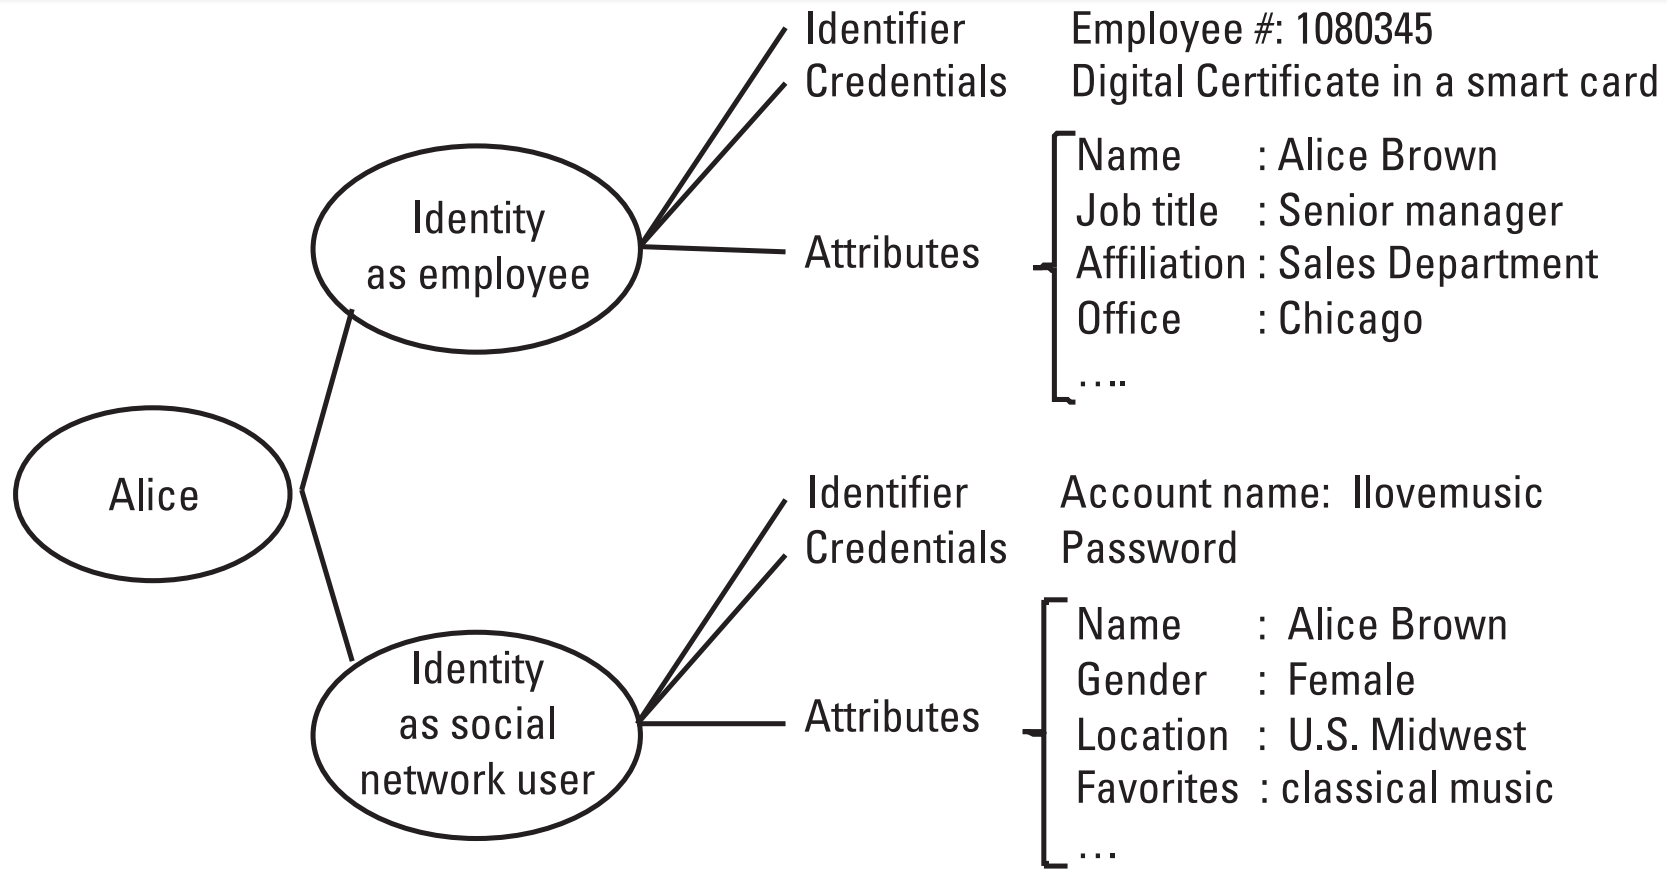
\includegraphics[width=0.8\linewidth]{images/Identity_Definition.png}
    \caption[Structural View on the concept of (Digital) Identity]{Structural View on the concept of (Digital) Identity \cite{bertino2010identity}}
    \label{fig:identity_definition}
\end{figure}

\subsubsection{Identity Management Systems on the Internet}
\label{subsubsec:IdMSs}

Identity Management Systems (IdMSs) are essentially a framework with a predefined set of rules on how digital identities are meant to be commissioned, managed and revoked. In this section light will be shed on the current implementations available to store and manage identities on the Internet, dividing it between two paradigms: Traditional and Decentralized IdMSs.

\paragraph{Traditional IdMSs}

The way Traditional Identity Management Systems were designed was on the basis of three or four actors: Subjects, \glspl{RP}, \glspl{IdP} and in some cases \glspl{CP} \cite{bertino2010identity}. Note that depending on the literature the nomenclature for "Relying Parties" has other definitions such as "Service Provider" \cite{zhu2018identity}. The traditional IdMSs are mainly dependent on a centralized IdP that performs operations of creating, updating, managing and deleting identities of users \cite{gebresilassie2020distributed}. To understand clearly what each party represents, a description extracted from the book by Bertino and Takahashi (2010) \cite{bertino2010identity}, can be found below.
\begin{itemize}
    \item "\textbf{Subjects} are the parties whose identity attributes are digitally recorded and used for transactions and other purposes."
    \item "\textbf{Identity Providers} are the parties that provision identities to subjects."
    \item "\textbf{Relying parties} are the parties that in order to provide services to users (or agents on behalf of users) or access to resources require the submission of proper credentials by users."
    \item "\textbf{Control parties} are typically law enforcement agencies and regulatory bodies that may need access to identity information."
\end{itemize}

The way these parties interact with each other can be summarized using the communication diagram shown in Figure~\ref{fig:interactions_between_different_parties} where it is clear the flow of information between Subjects, RPs and IdPs. Note that since most IdMSs do not require a CP, it has been exempt from this example, but if placed in the diagram it would fall in the center of the triangle and would communicate with all parties as it acts as a regulatory party. The parties depend on each other in the following way: the subject requests access to services from the RP, which in turn requires the IdP to challenge the subject identity through the authentication protocol \cite{zhu2018identity}.

At the dawn of identity management, the solution was truly centralized, since the RPs and the IdPs are combined into one unique entity that acts as the resource server while holding the username and password. This way, traditional identity management models face many challenges including the fact that they rely on a centralized architecture, which in turn leads to single-point-of-failure faults. Also these architectures are more prone to common attacks (e.g. Distributed Denial of Service) given there is a centralized server that can be targeted. Furthermore, in an IoT scenario scalability issues arise, also due to centralization issues. Lastly, and given that most things happen under-the-hood, most systems operate in a non-transparent manner \cite{gebresilassie2020distributed}. This lifts privacy matters, since the users are not fully aware of the practices of an organization, which for example might include their data being sold to 3rd parties.

\begin{figure}[!ht]
    \centering
    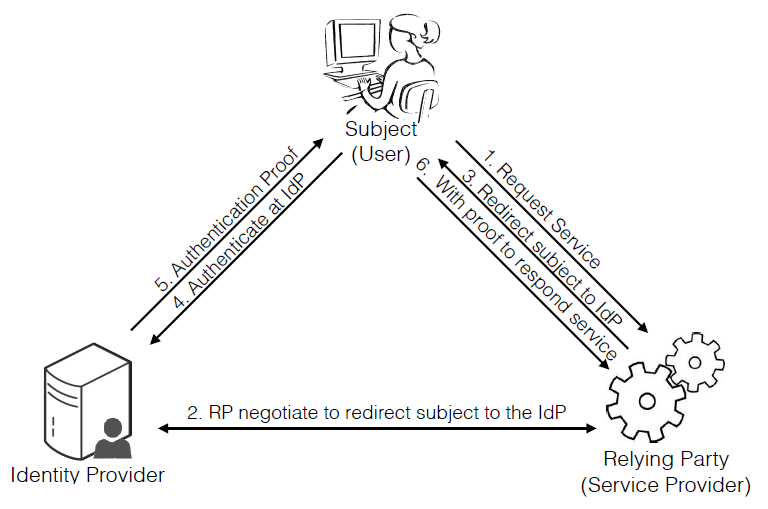
\includegraphics[width=0.6\linewidth]{images/simplified_traditional_IdMS.png}
    \caption[Interactions between different parties in a traditional IdMS]{Interactions between different parties in a traditional IdMS \cite{zhu2018identity}}
    \label{fig:interactions_between_different_parties}
\end{figure}

There is not a single model on how to utilize the Traditional IdMSs. There are four (4) different definitions of models: Isolated, Centralized, Federated and User-Centric. Depending on the systems requirements, a different model is used. However, in general terms, the past IdMSs have evolved from isolated to centralized, and then to federated/user-centric models \cite{JosangAuscertconference}.

\textbf{Isolated Models} are similar to what the web reassembles to today in its majority. Users create different identities for each service they use (mostly usernames and passwords) and they are required to memorize each different identity since the IdP and the SP are combined into one. For example, Facebook creates the identity of the user, but also manages it and manipulates it as they wish (according to regulations).
Since it is up for the users to memorize their identities, and since each service requires different parameters of security (e.g. password must contain 12 characters, 5 numbers and the square root of $\pi$) this can possibly lead to mismanaging identities, password reuse and forgetting credentials \cite{gebresilassie2020distributed}. 

\textbf{Centralized Models} differs from the Isolated Model since it makes use of \acrfull{SSO}, enabling multiple SPs under the same authority to make use of a single IdP. This helps reducing the number of credentials a user needs to memorize, but adds the security liabilities of having a single point of failure, lack of scalability and also introduction to other vulnerabilities and attacks.

\textbf{Federated Models} are similar to Centralized, with the exception that instead of having one authority that controls the Single Sign-On, a consortium of authorities agree with one login that serves for many different services, hence reducing credential management on the user side.

\textbf{User-Centric Models} are more aligned with the need to shift to a paradigm that puts governance in the hands of the users who own the data. This model revolves around users storing the credentials they have in either smart cards or smartphones, but still having the credentials stored in a centralized system provided by the SP. Although it was a step in the right direction it still suffered from the issues causes by relying on a centralized architecture.

\paragraph{Decentralized IdMSs}

With problems such as single point of failure of a centralized IdMS, the privacy concerns that have been reported (Facebook and Equifax data breaches \cite{zhu2018identity} \cite{van2019self} \footnote{\url{https://files.iota.org/comms/IOTA_The_Case_for_a_Unified_Identity.pdf}}), the approach shifted to a decentralized alternative. This approach has in its core the concept of using blockchain, a type of \acrfull{DLT}.

Blockchain was first introduced by Satoshi Nakamoto in the Bitcoin Whitepaper \cite{nakamoto2019bitcoin} and as been defined by the ISO standards as a "distributed ledger with confirmed blocks organized in an append-only, sequential chain using cryptographic links" \cite{ISO22739:2020(en)}. Blockchain consists of a decentralized structure composed of blocks which are linked together in a chronological order. In the Bitcoin implementation proposed by Nakamoto, a Proof-of-Work consensus algorithm is used, this reflects on how the transactions within each block are confirmed and how the blocks themselves get added to the chain. In this consensus mechanism that is allowed by miners who compute highly computational intensive tasks which in turn may return tokens. This latter statement is not the case for all blockchain implementations, but rather it was an example to highlight the usage of blocks and a consensus mechanism.

Blockchains can be of two types: permissioned, when the participants of the network are provided access to it, whereas in a permissionless implementation anyone can enter the network as a new node, which will hold the history of the blockchain, providing a decentralized way for data to be persisted \cite{s18082575} \cite{inbookWang}. 

With DLT it is possible to register every single transaction that gets added to the blockchain. Approaches have been made towards creating such decentralized IdMSs, which include the contributions of big companies such as IBM, and are good starting points for identity to be managed in a more private, secure and distributed way\footnote{\url{http://handle.itu.int/11.1002/1000/11559}}. 

\subsubsection{Paper Credentials Model}
\label{subsubsec:paper_credential_model}

Before diving into Self-Sovereign Identity and understanding how trust can be built around these concepts, it is important to realize how humans have been exchanging information and validating their claims in the past, and still to the time of writing. According to the Oxford Languages dictionary, credential is defined as a "qualification, achievement, quality, or aspect of a person's background, especially when used to indicate their suitability for something"\footnote{\url{https://www.lexico.com/definition/Credential}}. Essentially, a credential can be anything that proves that an individual is eligible for a particular ability (e.g. a driver's license card for driving). These do not need to take the format of a card, but it needs to be something that can bear a certificate that proves it was issued by a trusted party (e.g. the government hologram on the driver's license card). This way, any individual can guarantee that that credential is valid and legitimate. To put it simply, this model handles claims in a trust-based system, since there is no actual infallible method to prove a claim is real.
The basis for this system is composed of three (3) actors: An \textbf{issuer}, a \textbf{holder} and a \textbf{verifier}. Essentially their relationships are summarized in Figure~\ref{fig:paper_credential_model}, where it is clear that the issuer issues a credential to a holder, which when necessary will present it to a verifier. If the verifier trusts the entity which issued the document, it will acknowledge the holders claims as true. 

\begin{figure}[!htb]
    \centering
    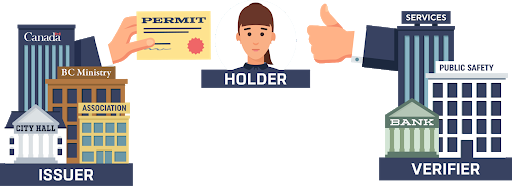
\includegraphics[width=0.7\linewidth]{images/The_Paper_Credential_Model.png}
    \caption[Paper Credential Model]{Paper Credential Model\protect \footnotemark}
    \label{fig:paper_credential_model}
\end{figure}

\footnotetext{\url{https://courses.edx.org/assets/courseware/v1/cb46ed78abdc7583aa95d011426676e0/asset-v1:LinuxFoundationX+LFS172x+3T2019+type\@asset+block/The_Paper_Credential_Model.png}}

At its early beginning (which reports back to the Persian era [Nehemiah 2:1–9]), it was primarily used to allow people with authorization to circulate between lands, provided they could show a document signed by an official authority. Due to the inability to forge documents and create fake copies of an official document, this model worked. But with time, and with the appearance of printers, scanners and software that allows image manipulation, the forging of documents became much easier. That leads to today's age, where the people who need to check for the authenticity of a document (the verifiers) need to be experts in the art of detecting forged credentials.

\subsection{Fundamental Concepts}
\label{subsec:fundamental_concepts}
%[Note: SSID definitely goes here]

In this section the most crucial concepts for this work are presented, with an emphasis on properly introducing the concept and the core enablers of Self-Sovereign Identity. A description of the updated Paper Credentials Model, named Verifiable Credentials Model is given. This is followed by a detailed explanation on the pillars of Self-Sovereign Identity, namely Decentralized Identifiers and the underlying communication protocol DIDComm, Verifiable Credentials and Zero-Knowledge Proofs. The \acrfull{W3C} has been developing specifications that are widely accepted as standards on these topics, and therefore the discussion will be based on these specifications, whose references will be contained in each section.

\subsubsection{Self-Sovereign Identity}
\label{subsubsec:self-sovereign_identity}

\acrfull{SSI} is a key enabler of people being in charge of their own identities. Although it is a field which is still maturing as of the time of writing, it has been coined by Juniper Research as a field which will generate \$1.1 billion in annual revenue by the end of 2024.  \footnote{\url{https://www.juniperresearch.com/press/press-releases/self-sovereign-identity-to-be-a-billion-dollar}}

The term was deeply detailed in an article by Christopher Allen, where he provides a brilliant bridge between the IdMS topic covered before, and the field of SSI:

\begin{quote}
\textit{Self-sovereign identity is the next step beyond user-centric identity and that means it begins at the same place: the user must be central to the administration of identity. That requires not just the interoperability of a user’s identity across multiple locations, with the user’s consent, but also true user control of that digital identity, creating user autonomy. To accomplish this, a self-sovereign identity must be transportable; it can’t be locked down to one site or locale.}\footnote{\url{http://www.lifewithalacrity.com/2016/04/the-path-to-self-soverereign-identity.html}}
\end{quote}

SSI is set to become the next standard for internet communication, as it holds potential to solve many of the internet current trust issues. A brief overview of it can be coined in the following terms: Each entity becomes in charge of its own identity, which means that each user is capable of disclosing only the information and data which they deem relevant or necessary in any relationship they hold. Also, each entity is capable of revoking any piece of data from a relationship or even revoking a relationship entirely, without the need from the other party to consent to this \cite{lo2019analysis} \cite{10.1145/3384943.3409436}. It follows the path of the Decentralized IdMSs that were previously explained, since it utilizes a Distributed Ledger Technology (the blockchain), to enable the usage of \glspl{DID}, \glspl{VC} and enhanced cryptography to support other features such as \glspl{ZKP} \cite{bertino2010identity}. These concepts will be discussed in more detail in the following sections. With the core features mentioned above, SSI disables the need for a central authority to hold any data, and also provides a tamper-proof system that provides transparency and less possibility of forging any credential. Because of the underlying cryptography and blockchain technology, SSI means that an entity can present claims about its identity and others can verify it with cryptographic certainty \cite{liu2020blockchain}. 

\subsubsection{Verifiable Credentials Model}
\label{subsubsec:verifiable_credential_model}

While the Paper Credential Model worked for a long time, due to its many issues with possible forged documents (as documented in Section~\ref{subsubsec:paper_credential_model}), with SSI it is possible to implement the concept of the Verifiable Credentials Model. In 2019 the Verifiable Credential Model has been established as a standard by the W3C \cite{Zundel:19:VCD} \cite{kortesniemi2019improving}.

The foundation for this model is still the same as the Paper Credential Model, there are still 3 parties, namely the Issuer, Holder and Verifier, but a Verifiable Data Registry is added to the picture as a base truth for all the claims that are exchanged in the process.

In order to illustrate each role in this model, the following example will be described making reference to the roles and actions performed by a government, an individual and a vehicle rental agency, in the event of an individual wishing to rent a vehicle. 
The government (issuer) will emit a signed Verifiable Credential (or Claim) to the individual (holder) attesting that they are eligible to drive. The vehicle rental agency (verifier) will request proof that the individual (holder) is eligible to drive. The individual (holder) presents the claim to the vehicle rental agency (verifier), which will check in the Verifiable Data Registry whether the government (issuer) is an entity they trust. Given the claim is cryptographically signed, this prevents it from being a forged document, hence if the vehicle rental agency has the government as a trusted source, the individual has passed the verification process and may rent a vehicle. But, if at some point, the government revokes the individual's credential to be eligible to drive, if the user tries to present the revoked claim to the agency, the agency will know that the user's credential has been revoked. This is the major difference from the paper credential model, since there is no possible way to revoke a physical card which is in the possession of an individual.

A diagram highlighting the flow of interactions in the Verifiable Credentials Model is demonstrated in Figure~\ref{fig:VC_Model}.

\begin{figure}[h]
    \centering
    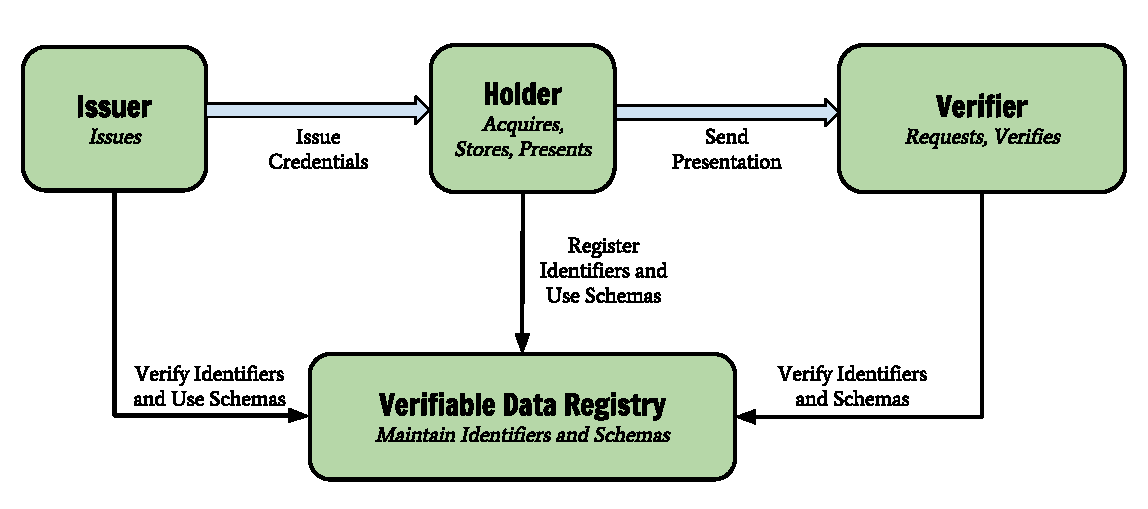
\includegraphics[width=0.7\linewidth]{images/VerifiableCredentialModel.pdf}
    \caption[The Verifiable Credentials Model]{The Verifiable Credentials Model \cite{Zundel:19:VCD}}
    \label{fig:VC_Model}
\end{figure}

\subsubsection{Decentralized Identifiers}
\label{subsubsec:DIDs}

Decentralized Identifiers (DIDs) are the identifiers that power SSI solutions. The aim of this identifier is to provide a scalable way to securely identify each identity that needs to be created. A DID is created for each entity and can be resolved by means of a DID Resolver, which can be seen as the DNS of SSI. Whenever a DID is resolved, it will unveil a DID Document (DIDDoc), which will hold a public key and an endpoint for the other entities to send messages to, allowing them to request for connection establishment  \cite{10.1145/3384943.3409436}. An architectural overview of this process can be found in Figure~\ref{fig:DID_architecture}.
There are two forms of DID, public or pairwise DIDs. While the first is meant to be used by entities that are meant to be "public" and widely contacted (for example a government branch), the latter provides a more secure channel for two entities to connect between each other. The difference between the two in regards to implementation is that Public DIDs are stored in a verifiable public data registry (the blockchain), allowing any entity to have access to this DID. Any individual can request to connect to the entity whose DID is public by creating a connection request. Pairwise DIDs are meant for more secure communication, since for each connection between two different entities, the data for these communications is stored locally, safeguarding from any other entity from eavesdropping, while also reducing the time to start of a connection \cite{terzi2020securing} \cite{theodouli2020towards}.
One of the strongest points with regards to DIDs are that at any time, a DID can be revoked by one of the parties, not allowing for other entities who know this DID to connect to this entity through it. If they wish to do so they must request a new DID for a new relationship to be established \cite{fedrecheski2020self}.

\begin{figure}[t]
    \centering
    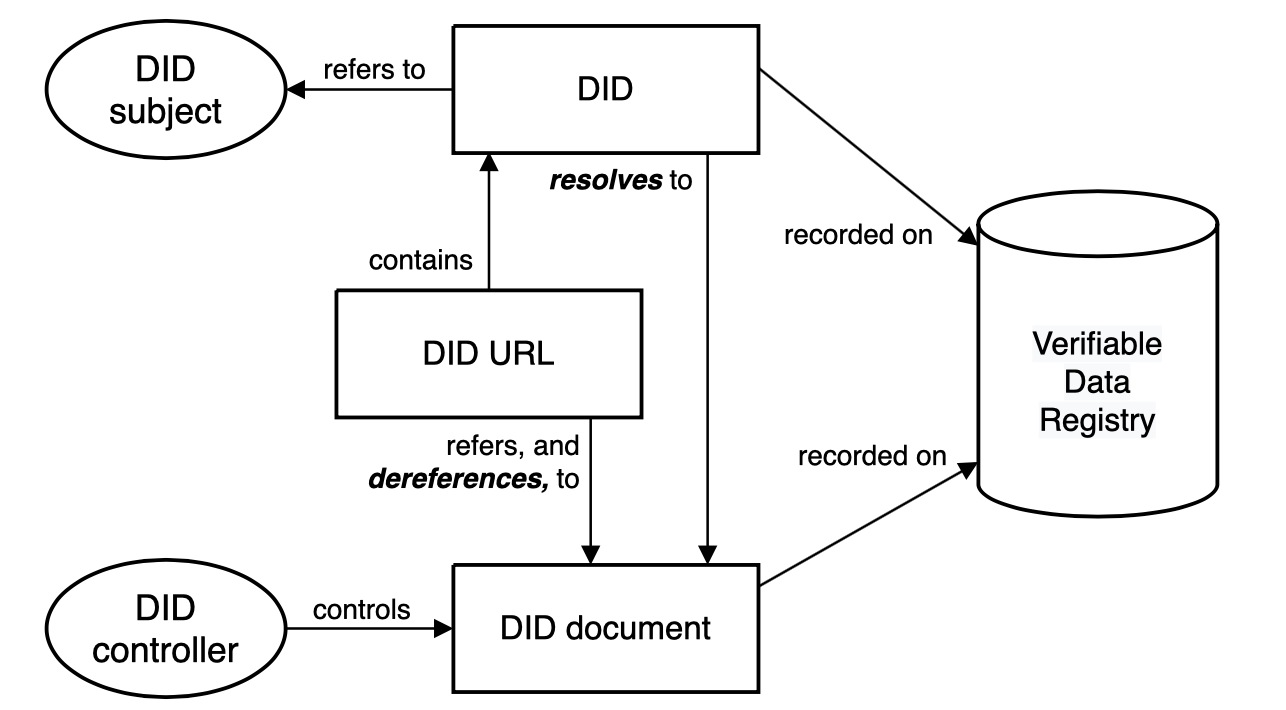
\includegraphics[width=0.6\linewidth]{images/did_brief_architecture_overview.png}
    \caption[Overview of DID architecture]{Overview of the DID architecture \cite{Longley:21:DI}}
    \label{fig:DID_architecture}
\end{figure}

A DID is similar to a universally unique identifier (uuid) for one's identity. Depending on the method used to create the DID, the structure will vary\footnote{\url{https://www.w3.org/TR/did-core/\#did-syntax}}. An example of a DID from the Sovrin network that is going to be discussed further in Section~\ref{subsubsec:hyperledger_indy_sovrin} can be found below:

\begin{verbatim}
    did:sov:AKRMugEbG3ez24K2xnqqrm
\end{verbatim}

The format of the DID follows the standard listed in the official documentation\footnote{\url{https://github.com/WebOfTrustInfo/rwot3-sf/blob/master/did-spec-wd03.md}} and the W3C specification \cite{Sabadello:21:DI}, where it specifies that the substring in between the commas refers to the DID method, which in this case would be of the Sovrin Network DID (\textit{sov}). At the time of writing there are 88 different DID methods listed in the W3C repository\footnote{\url{https://w3c.github.io/did-spec-registries/\#did-methods}}.

\paragraph{Messaging Protocol (DIDComm)}
\label{subsubsec:didcomm}

Although there are many different secure communication mechanisms as detailed in the survey conducted by Nguyen et al. in \cite{nguyen2015survey}, \acrfull{DIDComm}\footnote{\url{https://github.com/hyperledger/aries-rfcs/tree/master/features/0023-did-exchange}} differentiates itself, as it is defined as a protocol whose purpose is to provide a secure, private communication methodology built atop the decentralized design of DIDs\footnote{\url{https://identity.foundation/didcomm-messaging/spec/}}.

The methodology of DIDComm is based on the usage of the information that is present in the DID Documents to allow for secure,
private, decentralized, transport-agnostic, routable, interoperable, extensible, efficient communication between two individuals through their agents \cite{SovrinIotSSI}. 

The messaging format of DIDComm as defined by W3C uses JSON Web Messages\footnote{\url{https://identity.foundation/didcomm-messaging/spec/\#:~:text=DIDComm\%20plaintext\%20messages\%20are\%20based,message\%2C\%20and\%20are\%20called\%20headers.}}, and depending on the action to perform (issue credentials, request for a credential presentation, etc), the fields will vary. An example of a "Basic Message" structure would contain the following fields:

\begin{verbatim}
{   
    "id": "1234567890",
    "type": "<message-type-uri>",
    "from": "did:example:alice",
    "to": ["did:example:bob"],
    "created_time": 1516269022,
    "expires_time": 1516385931,
    "body": {"messagespecificattribute": "and its value"}
}
\end{verbatim}

\subsubsection{Verifiable Credentials}
\label{subsubsec:VCs}

Verifiable Credentials or Claims (VCs) are the pieces of technology in the digital world that mimic the physical credentials people bear with them on a regular basis like their passport, bank account number, amongst others. Verifiable Credentials are powered by digital signatures (powered by cryptography) making them verifiable and tamper-proof. The format of the VCs follows the standard listed by the W3C specification \cite{Sabadello:21:VCs}.

The way VCs can be adopted into people's lifes is by following the Verifiable Credentials Model previously mentioned in Section~\ref{subsubsec:verifiable_credential_model}. An example of how the fields (attributes) within the standard paper credentials can be ported to a Verifiable Credential is demonstrated in Figure~\ref{fig:example_VC}, where the Issuer Signature is missing since it refers to (in the example) the California Department of Motor Vehicles.
\begin{figure}[!htb]
    \centering
    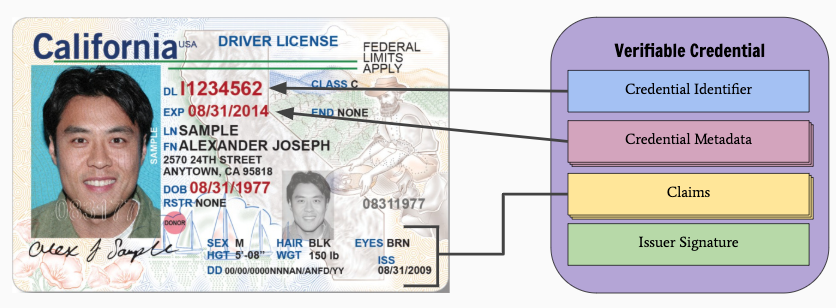
\includegraphics[width=0.7\linewidth]{images/Verifiable_Credentials.png}
    \caption[Example of how attributes from a paper crendential can be stored in a Verifiable Credential]{Example of how attributes from a paper crendential can be stored in a Verifiable Credential \protect\footnotemark}
    \label{fig:example_VC}
\end{figure}
In order to issue a credential, an issuer needs to use a credential schema that is present on the ledger, containing details on which information composes a credential under that schema.
\footnotetext{\url{https://freecontent.manning.com/the-basic-building-blocks-of-ssi}}
Whenever an issuer creates a schema, the ledger will create a response containing an identifier for that particular schema. If an issuer wishes to start issuing credentials under the schema listed above, they need to submit a credential definition onto the ledger mentioning the ID of the schema (provided earlier) and other fields like type of signature method, how to handle revocation and so on.\footnote{\url{https://hyperledger-indy.readthedocs.io/projects/sdk/en/latest/docs/how-tos/save-schema-and-cred-def/README.html}}

Figure~\ref{fig:relation_between_credential_schema_and_definition} holds an example of the link between a credential schema (which in the example is issued by the government), and the credential definition (who is created by an entity named "Faber"). Here is it possible to see how the credential definition contains the information regarding the schema as one of its fields. 

\begin{figure}[!htb]
    \centering
    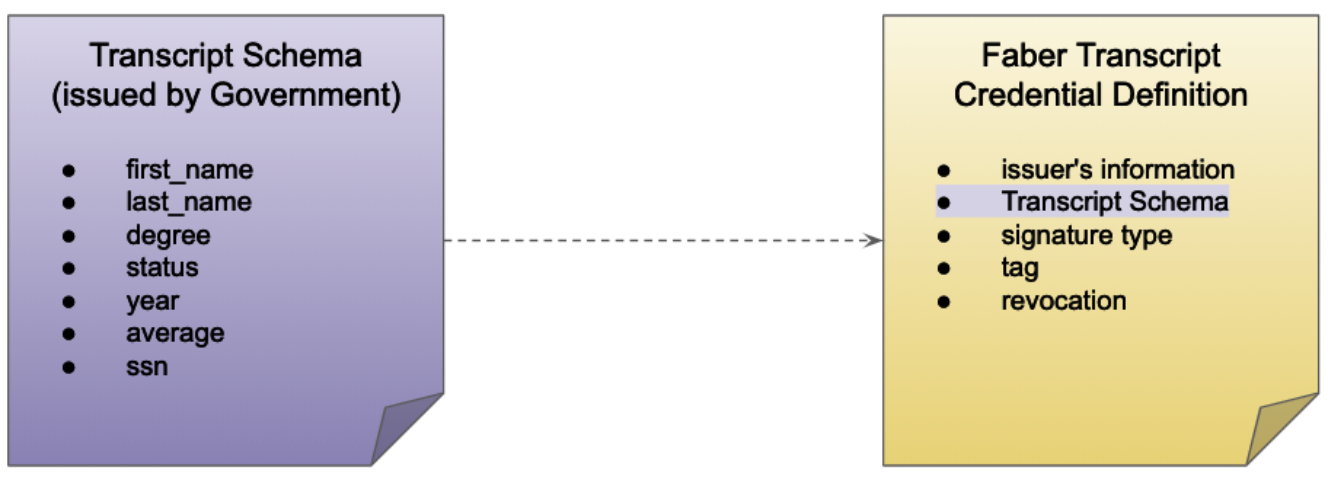
\includegraphics[width=0.7\linewidth]{images/schema-credential.png}
    \caption[Relation between credential schema and credential definition]{Relation between credential schema and credential definition \protect\footnotemark}
    \label{fig:relation_between_credential_schema_and_definition}
\end{figure}

\footnotetext{\url{https://kctheservant.medium.com/exploring-hyperledger-indy-through-indy-dev-example-10075d2547ae}}

Below an example of a credential object is presented, in the JSON Web Message format, containing the attributes, the credential\_definition\_id, revocation\_id and schema\_id.

\begin{verbatim}
    {
      "attrs": {
        "additionalProp1": "string",
        "additionalProp2": "string",
        "additionalProp3": "string"
      },
      "cred_def_id": "WgWxqztrNooG92RXvxSTWv:3:CL:20:tag",
      "cred_rev_id": "12345",
      "referent": "3fa85f64-5717-4562-b3fc-2c963f66afa6",
      "rev_reg_id": "WgWxqztrNooG92RXvxSTWv:4:WgWxqztrNooG92RXvxSTWv:3:CL:20:tag:CL_ACCUM:0",
      "schema_id": "WgWxqztrNooG92RXvxSTWv:2:schema_name:1.0"
    }
\end{verbatim}

\subsubsection{Zero-Knowledge Proof}
\label{subsubsec:ZKP}

The concepts of Zero-Knowledge Proofs is its majority powered by advancements in Mathematics and Cryptography and are one of the best ways to preserve individuals identities whenever they need to present any claim about themselves.
The moving force behind ZKP is the fact that an individual must not need to disclose any of its attributes in order to validate a claim. The Verifiable Credentials Model has already linked the implementation of ZKPs together with VCs in order to enable data minimization and privacy enhancement, as provers can present proof with minimal disclosure of sensitive and personal data to the verifiers \cite{terzi2020securing}\cite{Zundel:19:VCD}. To enhance privacy and security furthermore, the claims presented by the VC can take the form of a predicate ZKP or selective disclosure ZKP. 

\paragraph{Predicates in ZKP}

Predicates are used in ZKP whenever a holder needs to attest that he/she is in compliance with a requirement linked to one of its attributes without disclosing the data linked to that attribute \cite{bertino2010identity} \cite{bartolomeu2019self}. 
One of the predicates which is supported by VCs is the greater or equal to ($>=$). Using this predicate and formulating a real-life scenario would be for when an individual wants to demonstrate that he is over the age of 18 in order to request any alcoholic drink at a bar. Usually this process requires handing in the personal ID, in order for the barman to analyze the date of birth and calculate whether the individual is over the age of 18. With predicates in ZKP, the verifier (barman) would request proof that the individual (holder) is over the age of 18, which in turn would craft a Verifiable Presentation using ZKP, which can (by cryptographic means) validate that the user is older than 18, without ever disclosing the date of birth of the individual.

\paragraph{Selective Disclosure in ZKP}

Still picking up on the example of the individual who is required to demonstrate he is over the age of 18, despite that being a very ineffective process, it also discloses other information to the barman which are not relevant to that transaction. The ID is a Credential composed of many attributes which have relevance depending on the scenario. Hence, in a Verifiable Credentials Model using Selective Disclosure in ZKPs, a user can craft a presentation to show to the barman only the relevant piece of information (attributes) from a Verifiable Credential \cite{fedrecheski2020self}. This way the individual chooses to only disclose the date of birth from its ID in the form of a VC, and shows that newly crafted VC to the barman, without ever needing to disclose other pieces of data commonly found in a paper ID \cite{davie2019trust}. 

\subsubsection{Revocation of VCs}
\label{subsubsection:revocation_registries}

An issuer may want to revoke credentials, for the same reasons why paper credentials are revoked in the Paper Credentials Model: either they expire, or the holder lost privilege to hold them. Using the already mentioned driver's license example, if the driver loses too many points, the driver will be stripped off their driver's license so that they cannot drive anymore. With VCs, this event could be handled by revoking the credential that attests as the driver's license of the driver. In order to revoke a credential, the issuer of said credential writes a revocation registry and adds it to the Verifiable Data Registry. When revoked, the credential is no longer valid, and any verifier will be aware of this revocation by looking into the Verifiable Data Registry and being presented with the revocation registry of that credential.
The revocation registry links back to the credential, and allows the issuer to unilaterally revoke credentials, independently of the holders. Depending on the adopted DLT, the implementation for the revocation registry might differ\footnote{\url{https://tykn.tech/identity-revocation-blockchain/\#What_is_a_Revocation_Registry}}.

\subsubsection{Management of DIDs and VCs}
\label{subsubsec:wallets_and_agents}

An important aspect that was not yet discussed is how DIDs and VCs are handled and where they are stored. For this end, digital identity wallets, which are pieces of software purposefully created to store DIDs and VCs were envisioned\footnote{\url{https://freecontent.manning.com/the-basic-building-blocks-of-ssi/\#id_ftn4}}. On the other hand, in order to be part of the Verifiable Data Model and interact with other entities, there needs to be a piece of software that allows to manage and use the VCs that the entities hold in their wallets. That is the role of an agent, which can be defined as a software used by or acting on behalf of an entity to interact with other agents. Agents require access to a digital wallet in order to perform cryptographic operations on behalf of the entity that they represent\footnote{\url{https://sovrin.org/library/glossary/}}. 

Agents are in charge of sending and receiving messages; encrypting and decrypting information; sign digital information on behalf of the entity; manage information in the digital wallet and backup/restore information \cite{SovrinIotSSI}. The SSI community has advocated that an agent can also be referred to as a wallet, since most agents offer an integrated wallet as one of its components \footnote{\url{https://iiw.idcommons.net/Agent/Wallet\%3F_What_is_Agent\%3F_What_is_Wallet\%3F_Are_They_The_Same\%3F}}. This makes the two terms interchangeable in the literature.

Some agents contain the implementation to interact with the Verifiable Data Registry (i.e. Distributed Ledger), to allow for the adoption of the Verifiable Data Model. They can be of three different types: 

\begin{itemize}
    \item Edge agents run at the edge of the network on a local device;
    \item Cloud agents run remotely on a server or cloud hosting service
    \item Mobile agents are meant to be hosted on the entities' private device (e.g. smartphones)
\end{itemize}

The biggest difference worth denoting in the different types of agents is that cloud agents provide a public endpoint for interactions with other agents, with this endpoint being publicly available in the Verifiable Data Registry. Therefore, a person whose privacy is more important might be better using a mobile agent on their device, while an organization might have an agent running on the cloud. For IoT devices for example, it would be interesting to consider an edge agent as the preferred agent type. For the latter, lacking compute/storage resources and/or connectivity, securely communicating with a cloud agent that in turn communicates with the ledger \footnote{\url{https://github.com/hyperledger/aries-cloudagent-python/blob/main/docs/GettingStartedAriesDev/AriesBigPicture.md}} would be a possible alternative to the fact that these agents have no public endpoint.

\subsubsection{Relation with Distributed Ledger Technology}
\label{subsec:what_information_goes_onto_the_DLT?}

After covering DIDs and VCs, it is important to understand what gets stored on the Distributed Ledger. The most relevant note to be made is that no private data is stored on the blockchain, which provides any solution using a DLT with an increased privacy-preserving solution. The blockchain will only hold the Public DIDs, the Schemas, the Credential Definitions and the Revocation Registries. 

\subsection{Blockchain-based Self-Sovereign Identity with IoT}
\label{subsubsec:Blockchain-based_SSI_with_IoT}
%[Note: related work goes here]

In this section the related work will be discussed in detail, looking at the state-of-the-art research that has been put together with the aim of exploring Self-Sovereign Identity's integration into IoT environments.

For this purpose, the results from the numerous search queries are illustrated in Table~\ref{tab:related_work}. Note that for IEEEExplore and ACM (Digital Library), since these were extracted after Google Scholar, many of the papers listed under Google Scholar were also found repeated under the other two sources. The search terms utilized are listed in Table~\ref{tab:related_work_queries}.

\begin{table}[!ht]
    \centering
    \begin{threeparttable}[h]
        \begin{tabular}{|l|c|c|c|c|}
        \hline
            \backslashbox{Topic}{Source} & Google Scholar & IEEEExplore & DL & Other\tnote{1}\\
             \hline
            SSI + IoT & \cite{terzi2020securing}, \cite{gebresilassie2020distributed}, \cite{fedrecheski2020self}, \cite{bartolomeu2019self}, \cite{kulabukhova2019self} & \cite{theodouli2020towards} & \cite{10.1145/3352411.3352435} & \cite{kortesniemi2019improving}\\
            \hline
            SSI & \cite{van2019self} & \sout{ } & \sout{ } & \sout{ }\\
            \hline
            IdMSs for IoT & \cite{luecking2020decentralized}, \cite{zhu2018identity}, \cite{lo2019analysis}, \cite{10.1145/3384943.3409436}, \cite{liu2020blockchain},  \cite{zhu2017autonomic} & \sout{ } & \sout{ } & \sout{ }\\
            \hline
            SSI + Energy & \cite{cheddadi2020design}, \cite{dekker2020automating}, \cite{wang2019energy} & \sout{ } & \sout{ } & \sout{ }\\
            \hline
        \end{tabular}
        \begin{tablenotes}
        \item[1] Supervisor Literature, Back- and For-ward referencing.
        \end{tablenotes}
    \end{threeparttable}
    \caption{Summary of Literature}
    \label{tab:related_work}
\end{table}

\begin{table}[!ht]
    \centering
    \begin{threeparttable}[h]
        \centering
        \begin{tabular}{|p{0.2\linewidth}|p{0.7\linewidth}|}
        \hline
            \multicolumn{1}{|c|}{\textbf{Repository}} & \multicolumn{1}{c|}{\textbf{Search Terms}}\\
            \hline
            Google Scholar & "Self Sovereign Identity" \& "+"Self+Sovereign+Identity" +"Internet+of+Things" \& "Decentralized Identifiers"\\
            \hline
            IEEEExplore & "Self Sovereign Identity with IoT Blockchain" \\
            \hline
            ACM & "Self Sovereign Identity Internet of Things Blockchain" \\
            \hline
        \end{tabular}
        \begin{tablenotes}
        \end{tablenotes}
    \end{threeparttable}
    \caption{Literature Search Terms}
    \label{tab:related_work_queries}
\end{table}

\subsubsection{Blockchain as an IdMS}
\label{subsubsec:blockchain_as_an_IdMs}

The adoption of blockchain as a Decentralized IdMS has been widely acclaimed as a good alternative to handle access control as an alternative to the previous alternatives, namely ABAC (Attribute-based access control) and
RBAC (Role-Based Access Control), since it has been proved that these are inflexible, unscalable and difficult to upgrade \cite{liu2012authentication}. Despite blockchain-based IdMSs being coined the best alternative to traditional IdMSs \cite{10.1145/3352411.3352435}, these systems still present other issues compared to conventional IdMSs. Issues such as how to handle digital wallet leakage; identity changes; the underlying infrastructure and the key management of the public and private keys are some of the matters which need to be overcome in order to solidify blockchain as a definite substitute for traditional IdMSs \cite{liu2020blockchain}. 

\paragraph{Blockchain IdMS for IoT}

In a paper by Salah \cite{inproceedingsSalah} an analysis was made on different IoT access control approaches and the novel architecture based on blockchain proved to outperform OAuth2, OAuth0, Manual Device Authentication and Blockstack in the selected quality attributes (availability, scalability, decentralization and tamper-Proofness).

Being a distributed, incorruptible and tamper-resistant ledger database, blockchain has the potential to address the critical security issues of IoT, particularly on data integrity and reliability \cite{inbookWang}. 

However, not all types of blockchain are capable of serving IoT devices' needs. This is the case for permissionless blockchains, as they usually utilize proof-of-work consensus algorithms that are computationally expensive and involve high bandwidth overheads and delays. This in turn restricts the number of transactions per second that can occur \cite{luecking2020decentralized} \cite{lupascu2020dlt}. Hence, the best alternative is to utilize a permissioned blockchain for a possible IoT IdMS \cite{lo2019analysis}. 

The main challenges which need to be overcome in order to provide a standardized solution for IoT blockchain-based IdMSs are: computational power, energy demand and storage capabilities of IoT devices, mobility and partition of said devices and lastly the latency and capacity of communication to and from devices \cite{inbookWang}. On a survey conducted by Lo et al. \cite{lo2019analysis} more issues have been gathered regarding IoT devices and how these can affect a possible IdMS. Again, matters of resource consumption are identified with a scope on how encryption is made on the sensor data. Single point of failure, lack of standardization on managing IoT devices and interoperability are also matters related to IoT identified by this survey.

Matters of confidentiality, privacy and data integrity are also concerns in an IoT environment, and blockchain presents itself as a candidate for solving these issues. Blockchain grants authenticity, non-repudiation, and integrity by default, and if smart contracts are used to manage authorization and automate transactions, this satisfies the need for confidentiality, privacy and data integrity \cite{s18082575}. Despite the good prospects of blockchain, it still contains some drawbacks, such as ensuring security of computation, since the computational capability of blockchain is still limited; and also, due to the latency caused by some consensus algorithms on public blockchains, a system running with blockchain cannot support real-time monitoring \cite{lo2019analysis}.

The existing solutions for IoT blockchain-based IdMSs mostly represent generic solutions. However the domain-specific solutions regard the manufacturing domain, automotive, electric trading, energy grid, eHealth and smart home, according conducted surveys on the matter \cite{lo2019analysis}. One of the earliest architectures presented in 2017 referred to BIFIT, a system proposed for IoT smart homes to autonomously extract appliances signatures and create blockchain-based identity for the appliance owners, making use of an Ethereum smart-contract-based approach \cite{zhu2017autonomic}.

\subsubsection{Link between SSI and IoT}
\label{subsubsec:link_between_ssi_and_IoTIoV}

Although there are approaches mentioned in literature that relate to the usage of blockchain as an Identity Management System within an IoT environment, for the related work of this project the main scope is how the Self-Sovereign Identity concepts (DIDs, VCs, ZKPs) are put into practice in an IoT use case. Therefore, from the list of papers presented in Table~\ref{tab:related_work} the literature from line "SSI + IoT" will be analyzed in this section. Given that this field is currently maturing there are not many papers which specifically target the field of SSI with IoT, with the ones found reporting novel architectures or solutions, and some choosing to focus on the most urging challenges of integrating SSI with IoT or reflect on the benefits of SSI in detriment to the current implementations. In order to summarize the captured key benefits mentioned in the analyzed papers and also the challenges that need to be overcome in order to align SSI concepts with IoT, two tables are presented for such purposes, Table~\ref{tab:benefits_SSI} and Table~\ref{tab:challenges_SSI}, respectively.

The paper provided by Bartolomeu et al. \cite{bartolomeu2019self} reflects on the use cases, technologies and challenges of SSI for Industrial IoT. In this paper the authors provide a detailed comparison on the five different frameworks which focus on SSI, namely Hyperledger Indy, uPort, BlockStack, VeresOne and Jolocom (to be discussed further in the following section). The challenges reported by the paper illustrate the major issues with implementing SSI in IoT (lack of development to date or changing the mindset and standards of developers and people). 

The paper by Fedrecheski et al. \cite{fedrecheski2020self} puts more focus in explaining the concept of SSI and comparing its Digital Identity models (DIDDoc and Verifiable Credentials) with other models such as PGP and X.509, and highlights that SSI has an all-around better structure to account for more scenarios, such as adding Semantic Schemas, ZKP and Selective Disclosure.

The remainder of the papers extracted as part of the related work comprise novel architectures which were developed to tackle specific issues. In the paper by Kulabukhova et al. \cite{kulabukhova2019self} a small discussion is made on which type of blockchain is the most indicated for the task at hand, presenting the likes of Bitcoin and Ethereum as non-viable options given the transaction costs inherent to those blockchains. On the other hand, this paper presents the IOTA Tangle (also to be discussed in the following section) as a viable option and expands it by demonstrating a possible architecture which could cover the likes of Logistic Chains. The proposed architecture does not comply entirely with the SSI concepts, since they propose that the user's mobile wallet acts as the  identity provider. Then, if the user wants to use SSI he would require the usage of his local identity from a centralized IdMS to interact, which defeats the purpose of SSI.

In the paper by Terzi et al. \cite{terzi2020securing} an in-depth analysis is made on how to utilize SSI in order to guarantee that the emission rates produced by Internet of Vehicles (IoV) devices (a sub-type of IoT devices) are verifiable and untampered. From the related work research conducted, this paper is the one which more deeply relates to the task aimed with this project, since it also focuses on IoT directed towards the automotive domain. The team behind the paper integrated Hyperledger Indy to authenticate and authorize entities on a Hyperledger Fabric network. Their approach puts authorities as issuers who have write-access to the ledger, allowing them to register the vehicles and issue credentials. The paper reinforces that the emissions data is sent periodically (every 24h) and are stored in the Hyperledger Fabric blockchain. The paper also illustrates the sequence of interactions between a vehicle and a credential provider in order for the vehicle to hold a Verifiable Credential to attest that the vehicle is compliant with regulations.

In the paper by Gebresilassie et al. \cite{gebresilassie2020distributed} more emphasis is put into how to manage the identity within a SSI context. Essentially the paper reflects on the current IdMSs and provides some guidance on the IdMSs that can provide a decentralized approach (powered by SSI). The paper covers the likes of uPort, Hyperledger Indy and a project named ADEPT (which at the time of writing has been deprecated). Then the authors propose a novel approach based on the IOTA Tangle aimed at solving a vehicle rental agency use case, which has not been tested to date.

In the paper by Kortesniemi et al. \cite{kortesniemi2019improving} the main focus is on providing privacy for IoT devices. This paper sheds light on the DIDs covered in Section~\ref{subsubsec:DIDs}, demonstrating how it can reduce correlation between parties, which in turn improves the privacy of a system making use of DIDs.

\begin{table}[!ht]
    \centering
    \begin{tabular}{|p{36mm}|cccc|}
    \hline
         \backslashbox[40mm]{Benefits}{Literature} & Bartolomeu et al. & Fedrecheski et al. & Kortesniemi et al. & Gebresilassie et al.\\
         \hline
         Owner-Centric & X & X & & \\
         Privacy-preserving & X & X & X & X \\
         Decentralized & X & X & X & X\\
         End-to-end security & & X &&  \\
         Layered authentication & X & X & & \\
         Standardized and open approach & & X & X & \\
         JSON-based encoding & & X & & \\
         Scalability improvements & & & & X \\
         \hline
    \end{tabular}
    \caption{Captured Benefits of SSI in the literature}
    \label{tab:benefits_SSI}
\end{table}

\begin{table}[!ht]
    \centering
    \begin{threeparttable}[h]
        \centering
        \begin{tabular}{|p{36mm}|cccc|}
        \hline
             \backslashbox[40mm]{Challenges}{Literature} & Bartolomeu et al. & Fedrecheski et al. & Kortesniemi et al. & Lo et al. \\
             \hline
             Technical\tnote{1} & X & X & X & X\\
             Best Practices and Standardization & & X & & X\\
             Organizational and Applicational & & X & & X \\
             Software availability & X & & &\\
             \hline
        \end{tabular}
        \begin{tablenotes}
        \item[1] Constrained devices; Asymmetric Cryptography; Communication overhead; DID Resolution.
        \end{tablenotes}
    \end{threeparttable}
    \caption{Captured Challenges of incorporating SSI with IoT in the literature}
    \label{tab:challenges_SSI}
\end{table}

\iffalse
\begin{center}
Querying \textbf{} on Google Scholar + supervisor provided literature
5 papers on SSI with IoT 
5 papers on Identity Management Frameworks for IoT (with or without blockchain)
1 paper + 1 protocol whitepaper on SSI
3 papers on SSI/blockchain usage on the energy domain

IEEEExplore using query "\textbf{}" yielded 5 results:
1 papers has been added to the list of literature under SSI with IoT
\cite{theodouli2020towards}
3 had been already gathered in the previous round of literature gathering
1 paper was discarded due to lack of access rights

Refining my search on Google Scholar under the terms "\textbf{}" provided me with 8 papers, from which one was added to the list of literature under "SSI" and from the other 7, 3 were repeating results from the IEEEExplore query, and 4 were discarded since they did not relate to the topic closely or focused on other aspects which are not relevant for the research.

ACM query \textbf{} under the surveys tab provided me with yet another survey on the topic. \cite{10.1145/3352411.3352435}

Then by searching for \textbf{Decentralized Identifiers} (a search team highly correlated with SSI), I obtained a paper which has an implementation of Decentralized Identity Framework for IoT, that holds many thorough explanations of the concepts I cover in the background of my thesis. \cite{10.1145/3384943.3409436}
\end{center}
\fi

\newpage

\subsection{Existing Technologies}
\label{subsec:existing_technologies_and_application_domains}

In this section the most prominent technologies for the purposes of SSI with IoT integration will be explained, according to the time of writing. Most of the focus will be put into how these technologies are contributing directly or indirectly to put in practice the concepts of Self-Sovereign Identity and the Verifiable Credentials Model.

In Table~\ref{tab:frameworks} it is possible to see the different frameworks that have been detected in the literature, either from actual implementations or from experimenting with said frameworks. In the following sections the most occurring frameworks will be analyzed, to understand whether they are still viable alternatives for SSI implementations.

\begin{table}[!ht]
    \centering
    \begin{tabular}{|p{36mm}|cccccccccc|}
    \hline
         \backslashbox[40mm]{Frameworks}{Literature} &  \cite{luecking2020decentralized} &	 \cite{terzi2020securing} 	& \cite{zhu2018identity} &	 \cite{gebresilassie2020distributed} &	 \cite{inbookWang} &	 \cite{lo2019analysis}	& \cite{liu2020blockchain} 	& \cite{theodouli2020towards} & \cite{bartolomeu2019self} &	 \cite{kulabukhova2019self} \\
         \hline
              Hyperledger Indy/Sovrin  &     &  X  &  X  &  X  &      &     &  X  &  X  &  X  &  X  \\
             IOTA Tangle               &  X  &     &     &  X  &  X   &  X  &     &     &     &  X  \\
             uPort                     &     &     &     &  X  &      & ~   &  X  &     &  X  &  X  \\
             BlockStack                &     &     &     &     &      & ~   &     &     &  X  &     \\
             Veres One                 &     &     &     &     &      & ~   &     &     &  X  &  X  \\
             Jolocom                   &     &     &     &     &      & ~   &     &     &  X  &  X  \\
             Civic                     &     &     &     &     &      & ~   &     &     &     &  X  \\
             Ontology                  &     &     &     &     &      & ~   &     &     &     &  X  \\
             Remes                     &     &     &     &     &      & ~   &     &     &     &  X  \\
             ADEPT                     &     &     &     &  X  &  X   & ~   &     &     &     &     \\
             ShoCard                   &     &     &     &     &      & ~   &  X  &     &     &     \\
             Bitcoin                   &     &     &     &     &  X   &  X  &     &     &     &     \\
             Ethereum                  &     &     &     &     &   X  &  X  &     &     &     &     \\
             Hyperledger Fabric        &     &     &     &     &  X   &  X  &     &     &     &     \\
             EOSIO                     &     &     &     &     &  X   & ~   &     &     &     &     \\
             IPFS                      &     &     &     &     &  X   & ~   &     &     &     &     \\
             UCOT                      &     &     &     &     &  X   & ~   &     &     &     &     \\
             slock.it                  &     &     &     &     &   X  & ~   &     &     &     &     \\
             Power Ledger              &     &     &     &     &  X   & ~   &     &     &     &     \\
             MultiChain                &     &     &     &     &      &  X  &     &     &     &     \\
         \hline
    \end{tabular}
    \caption{Captured Frameworks in Literature}
    \label{tab:frameworks}
\end{table}

Looking at the results presented by Table~\ref{tab:frameworks}, the majority of the analyzed papers grasped Hyperledger Indy (7 out of 10), with the IOTA Tangle also getting some attention (5 out of 10). According to these results, a brief overview will be given on Hyperledger Indy and the IOTA Tangle, with an additional section reserved for the remainder of the frameworks mentioned in the table. This overview will mostly refer to the history of the framework and its current state.

\subsubsection{Hyperledger Indy / Sovrin}
\label{subsubsec:hyperledger_indy_sovrin}

At the time of writing and according to Table~\ref{tab:frameworks}, Hyperledger Indy / Sovrin Governance Framework is the most widely used framework for handling Self-Sovereign Identity. To provide some context, the Hyperledger Indy\footnote{\url{https://www.hyperledger.org/use/hyperledger-indy}} project is part of the Hyperledger ecosystem, hosted by The Linux Foundation, and its main aim is to provide an ecosystem to develop Decentralized Identity solutions. 
Sovrin is the name of the Foundation which essentially built its core network around the Hyperledger Indy framework. The Sovrin Foundation\footnote{\url{https://sovrin.org/four-pillars-of-an-ssi-network/}} is an active SSI network which is based around generous partners who willingly manage and take part in an SSI network, enabled by the Indy tools. Given that the Sovrin network is one of the most successful case studies built on the Hyperledger Indy ecosystem, the two terms have become interchangeable when referred in the literature.

\paragraph{From Indy to the Indy, Aries and Ursa Stack}

To summarize Hyperledger Indy's history, it started as a project which would handle all SSI related matters, from the DLT, the agents and the cryptography. The project has evolved over time since it launched in 2015, and a separation of concerns occurred, which brought to light two projects under the Hyperledger environment:

\begin{itemize}
    \item Hyperledger Aries\footnote{\url{https://www.hyperledger.org/use/aries}}, which would become a tool kit that included the Agent implementations.
    \item Hyperledger Ursa\footnote{\url{https://www.hyperledger.org/use/ursa}} was left responsible for all things related to cryptography and is now used in several Hyperledger projects who require cryptographic operations.
\end{itemize}

The Indy Distributed Ledger is characterized as a public, permissioned ledger and consensus is achieved using the Plenum algorithm \cite{terzi2020securing}. There are multiple deployments of Indy networks, but the most widely know is hosted by the Sovrin Foundation. It consists of a single, global instance of Hyperledger Indy that resembles to the identity equivalent of the Domain Name System (DNS). Hyperledger Indy nodes pool is an interconnected network of nodes that maintain the same state of the ledger by signing every communication using elliptic curve cryptography \cite{SovrinIotSSI}.

It is relevant to mention that the Indy DLT is composed of a DID registry, Claims Schemas and Credential Definitions, the Revocation Registries and at last the Key Management Component.

\subsubsection{IOTA Tangle/Identity}

The second-most mentioned framework in the gathered literature was the IOTA Tangle. IOTA\footnote{\url{https://www.iota.org}} itself corresponds to a cryptocurrency aimed at micro-payments for connecting human and machine economies and at providing blockchain solutions for IoT networks.

The IOTA Tangle is comparable to the blockchain technology, but with a twist. The Tangle consists of a Directed Acyclic Graph (DAG) structure, instead of Bitcoin's chain structure. Although the structure differs, the Tangle implementation still holds the anti-tampering benefits of blockchain \cite{s18082575} \cite{inbookWang}. When created, the Tangle network was designed to provide a platform for trusted communication between individuals, organizations and things. On top of Tangle, IOTA has developed a new solution named IOTA Identity\footnote{\url{https://www.iota.org/solutions/digital-identity}} prides on the use of the W3C's Verifiable Data Model standard for a digital identity framework. Their solution is described in their whitepaper, illustrating the concepts for a Self-Sovereign Identity framework (DIDs, VCs,...)\cite{IOTAIdentity}.

The Tangle is proven to be highly scalable \cite{luecking2020decentralized} \cite{gebresilassie2020distributed} \cite{s18082575} and is a network which requires no miners, eliminating miner fees, one of the possible restrictions of a scalable IoT blockchain \cite{s18082575} \cite{inbookWang}.
According to the implementation proposed by Luecking et al. the IOTA Tangle and its permissionless nature enables the creation of identities for IoT devices at any time without significant effort \cite{luecking2020decentralized}.
The security of IOTA as been discussed in Gebresilassie et al. and given that it uses Winternitz One-Time signature scheme for its encryption, the Tangle can withstand quantum attacks \cite{gebresilassie2020distributed}.

One possible drawback is mentioned in Kulabukhova et al. where the authors highlight that given the Tangle's design to use snapshots, these allow full nodes to remove a transaction history that comes before the actual snapshot transaction. Since this is happening a Public Key Registry could be eliminated easily \cite{kulabukhova2019self}.

Regarding IOTA Identity, although the whitepaper does provide an indication on the direction taken by the development team, there is an introduction of the topic and not presented solutions. Also, at the time of writing, the framework is still in Beta Release phase, having most of the core functionalities (credential exchange, revocation) still left not implemented, revealing some of the immaturity of the created framework. For these reasons, this framework will not be considered further by this work.

\subsubsection{Other Technologies}
\label{subsubsec:other_technologies}

In this section a few of the remainder technologies will be analyzed.
The uPort\footnote{\url{https://www.serto.id}} and Jolocom\footnote{\url{https://jolocom.io}} implementations were also mentioned in the literature quite often and are solutions which are open-source, allowing for a larger community to contribute to its development. 
One of its drawback is that they are based on the Ethereum blockchain, which endures in high cost-per-transaction and slower transaction-per-second times.
On top of that, the information on the credentials are stored in the form of hashes directly on the blockchain, which goes against the core principles of SSI listed in Section~\ref{subsubsec:self-sovereign_identity}, that mentions that Personally Identifiably Information (PII) should be held exclusively by its owner, and not stored in any place besides the owner wallet \cite{gebresilassie2020distributed}.



\section{Case Description and Requirement Elicitation}
\label{sec:requirement_elicitation}

In this chapter an overview will be given on the Case Study at hand. Alongside this description, light will be shed on the requirements to consider for further implementation and architectures.

\subsection{Case Description}
\label{subsec:case_description}

As covered in the previous sections of this project, Self-Sovereign Identity for IoT devices is a field which has yet to discover its full potential. Exploring the capabilities of SSI concepts in this field will allow further researchers to understand whether certain limitations of these environments caps the usage of DIDs, VCs and more SSI concepts. A field within the IoT scope which has seen an increase in demand in recent times, is the \glspl{EV} interactions. These type of interactions are included in a subset of the IoT devices, namely the IoV domain, which was already mentioned in Section~\ref{subsubsec:link_between_ssi_and_IoTIoV}.

The Case Study which will be the aim of this project is how to enable Self-Sovereign Identity within an EV Charging interaction, powered by Electric Vehicle Charging Stations. 

For the purpose of extracting information on the current architecture of the system, a domain expert was interviewed to assess the details of the current system, as well as to extract the requirements for a novel approach targeted for the same end. The following description of the system was developed over the span of several weeks and over a number of interactions with the expert, to match the details with the current reality of EV Charging.

A high-level overview of the system can be observed in Figure~\ref{fig:High-level overview}. In this diagram it is possible to see the involved parties as well as the types of communication some parties have between each other in the current system architecture. Alongside the diagram it is possible to see a legend with a description of the different parties.

The main goal of this work is to provide the benefits of Self-Sovereign Identity mentioned in Section~\ref{subsubsec:link_between_ssi_and_IoTIoV} into the Electric Vehicle Charging use case. Multiple parties will need to trust each other in order for an exchange of energy to take place. Making use of the Verifiable Credentials explained in Section~\ref{subsubsec:VCs} it is possible to guarantee that a vehicle belongs to a given owner, that the vehicle is itself, and several other claims which will be described later in this document.

More clarity will be given on the parties and their roles in the current system, and what types of communication occur in this system.

\begin{figure}[!htb]
    \centering
    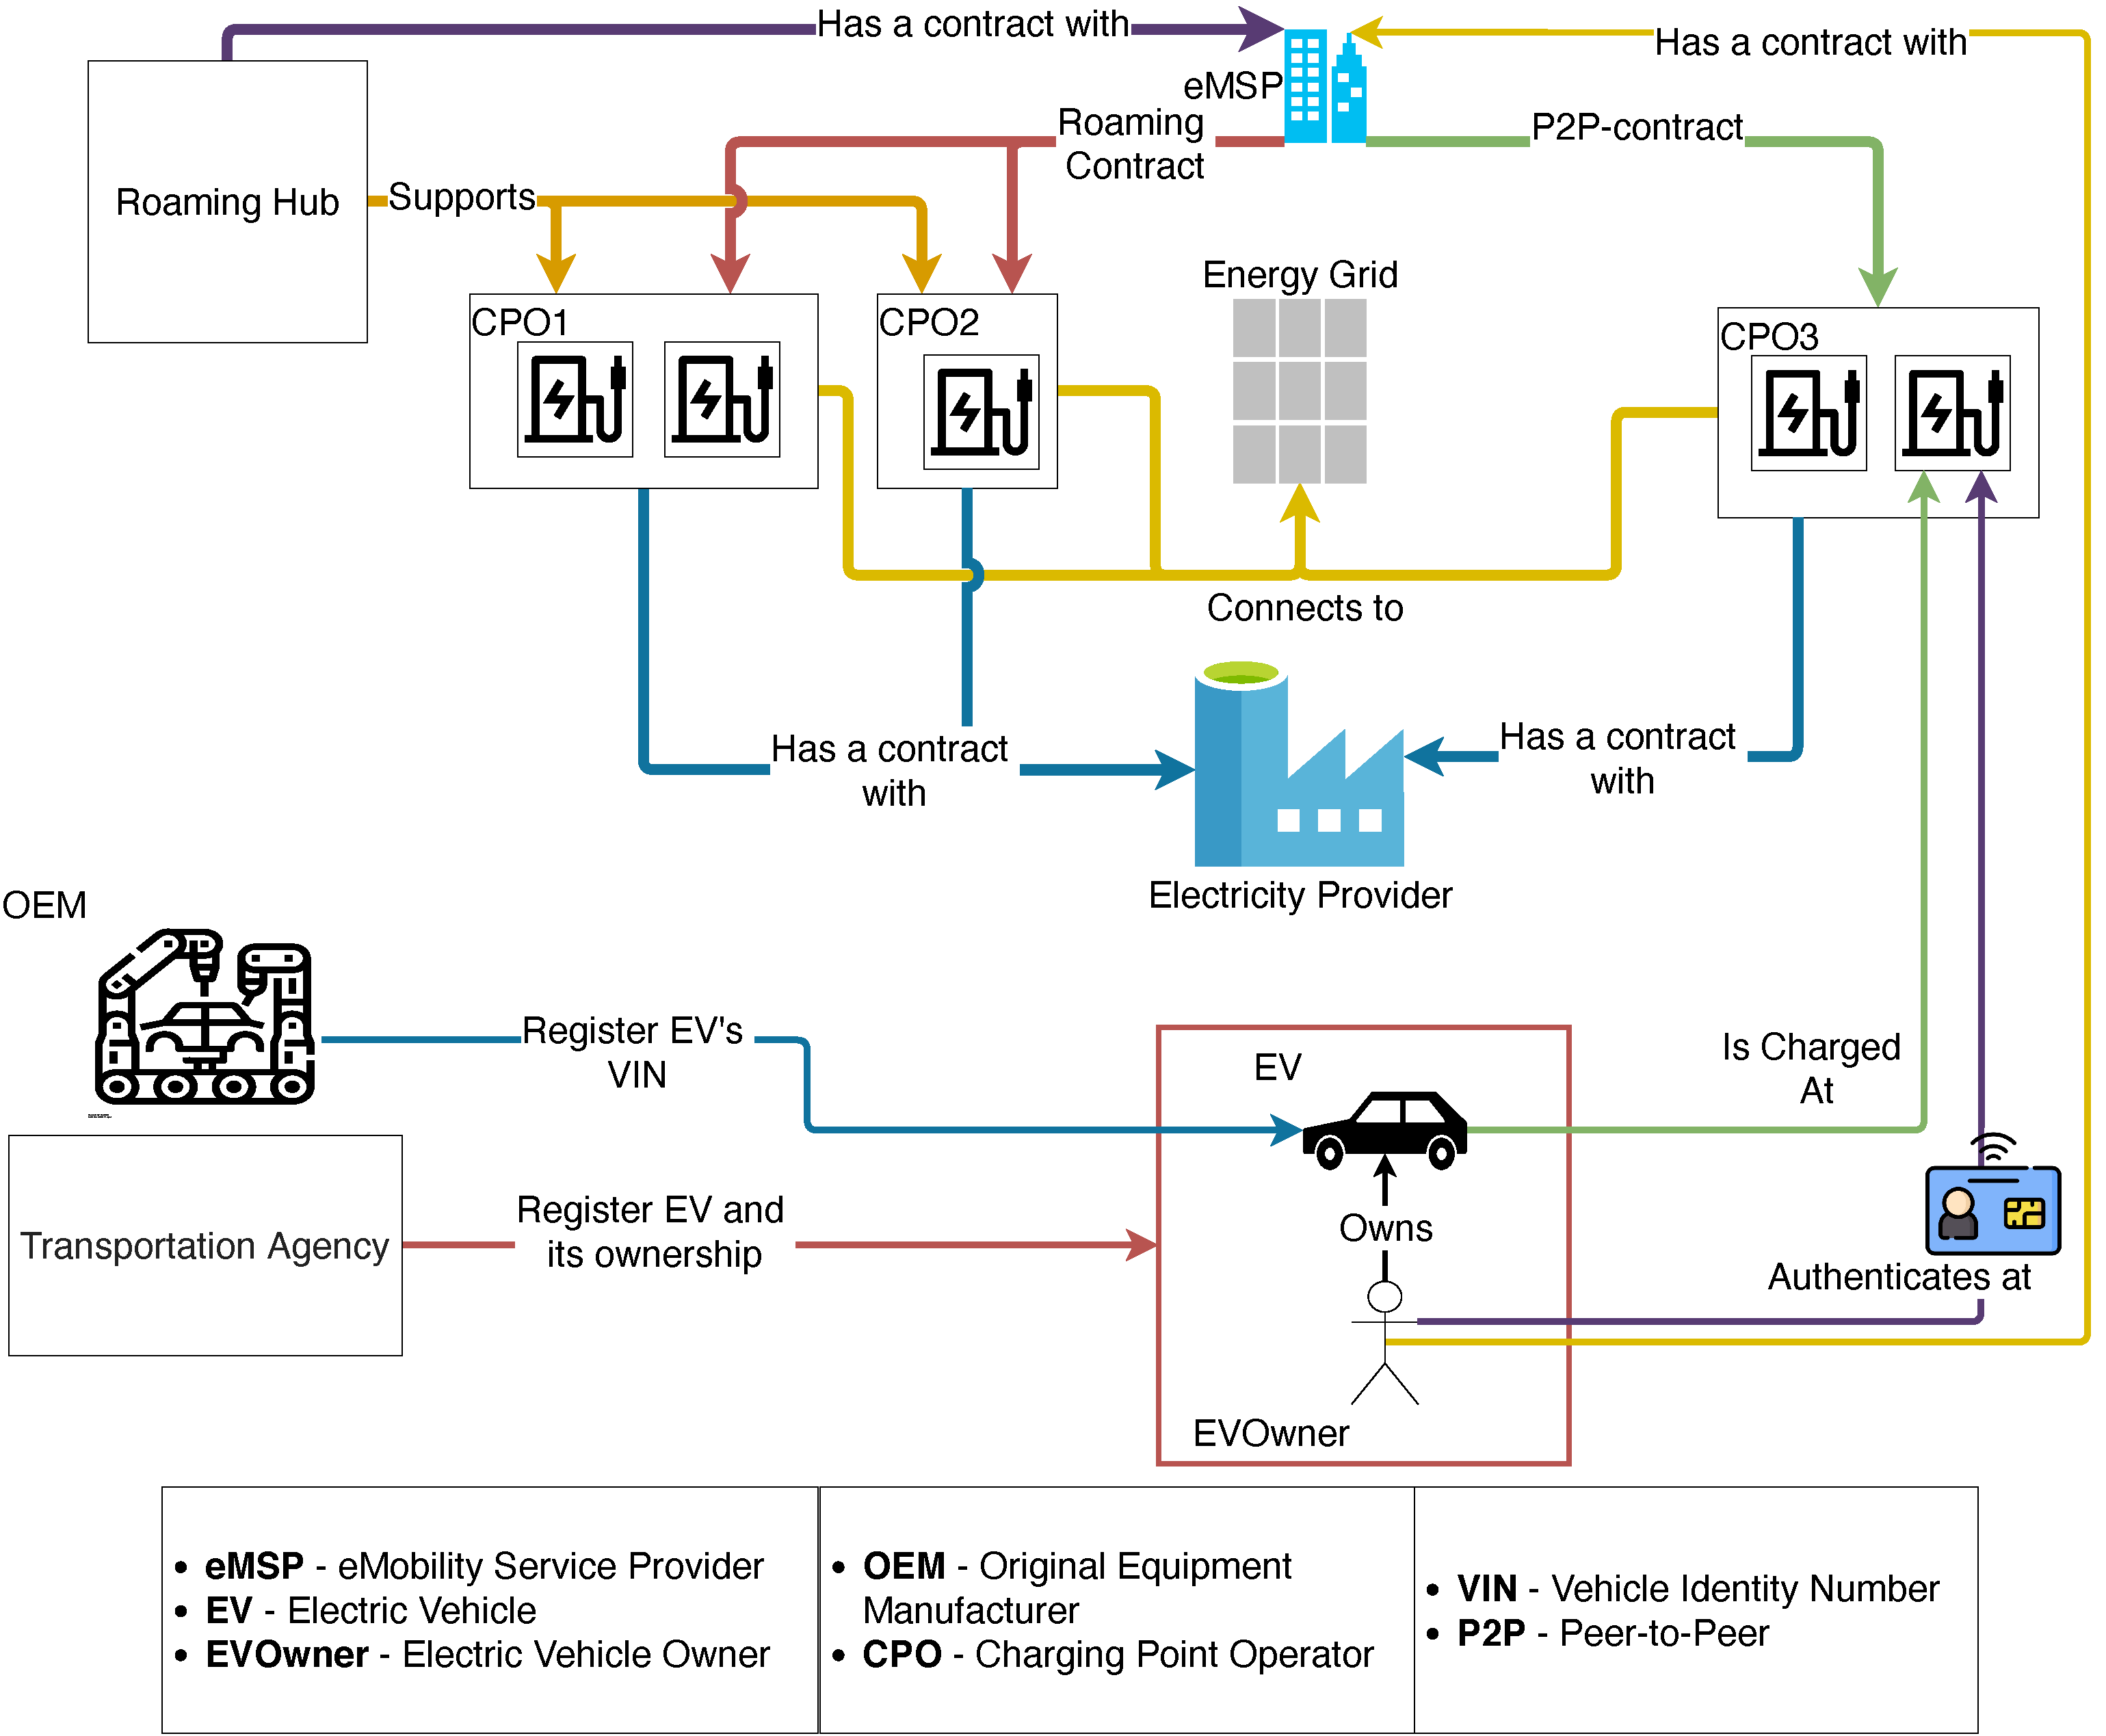
\includegraphics[width=0.85\linewidth]{images/Initial_model.pdf}
    \caption{High-level overview of Case Study}
    \label{fig:High-level overview}
\end{figure}

\subsubsection{Users and Information Flows}
\label{subsubsec:users_and_information_flows}

The diagram presented in Figure~\ref{fig:High-level overview} displays the parties that are involved in this case study, and how these connect between each other. The system comprises of three distinct flows: the "Service Providers", the "EV Owner and EV Interactions" and at last the "Charging and Billing".

\paragraph{Service Providers}

The primary party in this flow is an \acrfull{eMSP}, whose main goal is to provide the largest network of charging points available to its clients, the \glspl{EV Owner}. If an EV Owner wishes to charge their EV, there is the need to sign a contract with an eMSP (\textcolor{yellow}{Thin Yellow Line}).

In order to expand the network, the eMSP company may hire subsidiaries whose role is to act as a \acrfull{CPO}. These CPOs may have a Peer-to-Peer contract (\textcolor{green}{\textbf{Bold Green Line}}) or be part of Roaming Hubs of the company (\textcolor{purple}{\textbf{Bold Purple Line}}) and have a Roaming Contract (\textcolor{red}{\textbf{Bold Red Line}}). The CPOs are the ones that own the \glspl{CS} and are responsible for guaranteeing their good functioning. 
The CPOs are the ones who negotiate with the \glspl{EP} directly to obtain electricity for the Charging Stations (\textcolor{blue}{\textbf{Bold Blue Line}}). Additionally, the CPOs are the ones who directly communicate with the Energy Grid if one is to consider bilateral communication to balance the grid (Vehicle-To-Grid) (\textcolor{yellow}{\textbf{Bold Yellow Line}}).

In some occasions the eMSPs may have a preferred CPO contract, which in turn provides a cheaper price for EV Owners. In the occasion where the EV Owner tries to charge the vehicle in a different CPO (who also has a contract with the same eMSP), the fee may be larger. This also addresses another important point: when an EV Owner charges the EV at a new CPO, the CPO will not have the user credentials ready for authentication. When this happens the CPO may directly connect to the eMSP looking to authenticate the user; if this fails, the Roaming Hub will act as an intermediary between CPOs and eMSPs, in order to provide an alternative authentication route. Whenever an EV Owner wishes to charge their EV, the Roaming Hub will check whether the user has been authenticated in one of the other CPOs in the Hub. This has an associated cost, since reaching to more parties means taking a longer authentication route.

\paragraph{EV Owner and EV Interactions}

In order for an EV to be driven by someone, it requires documentation to attest a vehicle's unique identifier, which is named \acrfull{VIN} and may be contained in a \acrfull{VBC}, and whose issuer is the respective \acrfull{OEM} (\textcolor{blue}{Thin Blue Lines}).

For someone to charge their vehicle they must be the owners of said vehicle\footnote{This is a simplifying assumption for the purposes of this work and in reality this assumption does not always hold (e.g. when lending the vehicle to a relative, or when being the owner of a vehicle rental agency, more on this will be covered in the evaluation chapter)}. This means that the EV Owner and the EV must be registered together in the \acrfull{TA} of the respective country (RDW or "Rijksdienst voor het Wegverkeer" in the Netherlands) so that an EV Owner is legally allowed to drive their EV on the roads (\textcolor{red}{Thin Red Lines}).

\paragraph{Charging and Billing}

After the contract with the eMSP is signed (as mentioned in the "Service Providers" flow), the EV Owner may charge the EV at any of the CSs offered by CPOs who are contracted by the same eMSP. This requires the EV Owner to authenticate at the CSs using smart cards or login credentials on a mobile app provided by the eMSP for NFC authentication (\textcolor{purple}{Thin Purple Line}). Only if the authentication succeeds, the CS will start powering the EV (\textcolor{green}{Thin Green Line}). If an EV Owner tries to charge the EV at a CPO that does not have a contract with its eMSP, the charging is not possible.

The current system architecture's billing system comprises of the EV Owner making a monthly payment to the eMSP with the total of the expenses for the charging transactions in that given month. The CPOs obtain their profits from reselling the energy from the Electricity Providers to the EV Owners and also through a fees-model paid by the eMSP which is directly related to the number of EVs charging at the CPOs Charging Stations. The Roaming Hubs profit from providing an authentication route to the eMSPs, in case the CPOs have no past record of the user in the system. The EPs make profit from selling the energy directly to the CPOs with whom they have a contract.


\subsubsection{Current Liabilities}
\label{subsubsec:current_liabities}

In the current implementation of the Electric Vehicle Charging system, there are some liabilities which have been extracted based on the input provided by the domain experts. These include problems of transparency, security, data privacy and functionality.

\begin{itemize}
    \item The EV Owners are not aware of the price rate of the kWh at the time of charging, and are only aware of the total expense of one transaction when it is described in the monthly invoice. Consequently, CPOs have the chance to boost rates and the price of the energy sold to the EV Owners since the rates are not presented to the EV Owners before charging.
    \item Problems with current authentication is leading to identity fraud. With the usage of smart cards there is the chance for these to be cloned and used by malicious entities. With the usage of login credentials there is the problem with account hijacking which also leads to identity theft. Reports have been made for multiple charging sessions taking place far apart at close times, under the same identity.
    \item Still regarding authentication, in the current architecture the CPOs will try to authenticate the EV Owners by going directly to the eMSPs. If something goes wrong in this communication (e.g. fault in the network), and if the CPOs are contained within a Roaming Hub, they have the option to authenticate the EV Owners by means of those Roaming Hubs. When this occurs both CPOs and eMSPs are at a loss, given that the revenue is reduced by the introduction of a new party in this transaction (the Roaming Hub).
\end{itemize}

\subsection{List of requirements}
\label{subsec:list_of_requirements_and_decisions}

When designing a possible novel architecture, it is important to consider the current limitations in the field of SSI with IoT, and understand which technologies have the power to mitigate or erase such constraints. Also, given the current system architecture for the Charging of EVs, the requirements for that system should also be accounted for in a new architecture. Following the diagram presented in Figure~\ref{fig:High-level overview} which depicts an overview of the current system architecture, the requirements for a new architecture will be listed, followed by the respective rationales.

\subsubsection{Key Drivers}
\label{subsubsec:key_drivers}

In order to extract the key drivers of this system, an analysis on the literature was made in Section~\ref{subsubsec:Blockchain-based_SSI_with_IoT} to understand which are the most analyzed quality attributes when assessing SSI alone or together with its integration with IoT.

\paragraph{Scalability}

The literature highlighted as an urgent need that an SSI-based solution for IoT devices has the possibility to scale as the number of connected devices grow \cite{luecking2020decentralized} \cite{zhu2018identity} \cite{lo2019analysis} \cite{zhu2017autonomic}. The reason is evident, as mentioned in the introduction, the number of IoT devices is expanding and the need for a scalable IdMS is extremely important.

\paragraph{Performance}

Another important aspect to consider is the performance of the network. If the network contains low throughput, the number of \acrfull{TPS} may not satisfy the high volume of data collected by IoT devices \cite{lo2019analysis}. 

\paragraph{Security and Privacy}

Matters of data privacy, security and tampering are some of other aspects which need to be accounted when dealing with massive quantities of data and the identity of billions of IoT devices \cite{luecking2020decentralized} \cite{zhu2018identity} \cite{s18082575} \cite{theodouli2020towards}. These were matters addressed in literature which focused on an IdMS solution for IoT, which demonstrated to be sufficiently supported by blockchain solutions \cite{lo2019analysis}.

\paragraph{Other Relevant Quality Attributes}

While not key drivers, other quality attributes that were mentioned in the literature should also be taken into account when designing a new system architecture. Interoperability \cite{luecking2020decentralized} \cite{zhu2018identity} and availability \cite{theodouli2020towards} are examples of other NFRs which will also be considered in the selection of the components of the new systems architecture.

Regarding the availability of the system, according to Transport \& Environment, Europe's leading clean transport campaign group, a system whose goal is to provide electric vehicle charging stations to clients requires a 97\% uptime guarantee, according to the latest published report \cite{todts_2020}.

\subsubsection{Functional Requirements}

The \glspl{FR} displayed in Table~\ref{tab:functional_requirements} relate to the technical functionality of the Electric Vehicle Charging system, and are organized to better display what each functionality will add to the system. The requirements have been categorized using the MoSCoW prioritization technique\footnote{\url{https://www.productplan.com/glossary/moscow-prioritization/}}, where each requirement is tagged with one of the following levels of priority: "Must have", "Should have, "Could have" and "Will not have".

\begin{longtable}{|p{.1\textwidth}p{.15\textwidth}p{.70\textwidth}|}
    \hline
    \textbf{ID} & \textbf{Priority} & \textbf{Requirement}\\
    \hline
    \hline
   \textbf{FR-1.1} & Must & \textit{The system must allow for an EV Owner to charge its EV at a CS}\\
   \textbf{FR-1.2} & Should & \textit{The rate at which the kWh is being sold to the EV Owner should be presented before the charging starts}\\
   \textbf{FR-1.3} & Must & \textit{The EV Owner must be prompted to accept/reject the price of the kWh}\\
   \textbf{FR-1.4} & Could & \textit{At the end of a transaction, the EV Owner could receive proof of the transaction with the amount due}\\
   \hline
   \textbf{FR-2.1} & Must & \textit{A CS must belong to a CPO}\\
   \textbf{FR-2.2} & Must & \textit{A CPO must have a contract with an eMSP}\\
   \textbf{FR-2.3} & Must & \textit{A CPO must have a contract with an EP to provide power to its Charging Stations}\\
   \hline
   \textbf{FR-3.1} & Should & \textit{EV Owners should prove they are the owners of their EV to a CS}\\
   \textbf{FR-3.2} & Must & \textit{EV Owners must attest they have a valid contract with an eMSP that the CS's CPO has a contract with}\\
   \textbf{FR-3.3} & Could & \textit{An EV Owner could be made aware that the CS belongs to the CPO it claims} \\
   \textbf{FR-3.4} & Should & \textit{The process of setting up the connection and verifying credentials should be executed with the least EV Owner intervention as possible.}\\
   \hline
   \textbf{FR-4.1} & Must & \textit{An EV and the information regarding its EV Owner must be registered with the TA in order for the EV to be on the roads and to be charged at a CS}\\
   \hline
   \textbf{FR-5.1} & Must & \textit{The system must not write \acrfull{PII} in a publicly accessible data repository}\\
   \textbf{FR-5.2} & Must & \textit{Every credential issued must be verifiable using cryptographic proof}\\
   \hline
   \textbf{FR-6.1} & Must & \textit{An EV Owner must be able to delegate (temporary) possession of its EV to another driver}\\
   \hline
    \caption{Functional Requirements}
    \label{tab:functional_requirements}
\end{longtable}
    
\subsubsection{Non-Functional Requirements}

The \glspl{NFR} presented in this section are closely related to the key drivers identified in Section~\ref{subsubsec:key_drivers}. The key drivers act as important guidelines in the development of the system. The system-to-be aims to achieve the desired key attributes by fulfilling the non-functional requirements mentioned in Table~\ref{tab:non-functional_requirements}. The requirements have been categorized using the MoSCoW prioritization technique \footnote{\url{https://www.productplan.com/glossary/moscow-prioritization/}}, where each requirement is tagged with one of the following levels of priority: "Must have", "Should have, "Could have" and "Will not have". 
Each set of requirements directly links to a key driver according to the following match: 

\begin{itemize}
    \item \textbf{NFR-1.X} - Scalability
    \item \textbf{NFR-2.X} - Performance
    \item \textbf{NFR-3.X} - Security and Privacy
    \item \textbf{NFR-4.X} - Other Relevant Quality Attributes
\end{itemize}

\begin{longtable}{|p{.1\textwidth}p{.15\textwidth}p{.70\textwidth}|}
        \hline
        \textbf{ID} & \textbf{Priority} & \textbf{Requirement}\\
        \hline
        \hline
       \textbf{NFR-1.1} & Must & \textit{The system must scale according to the growth of the market. Supposing an adoption in the Dutch Market (300k EVs in 2020 \protect\footnotemark)     \footnotetext{\url{https://www.rvo.nl/sites/default/files/2020/11/Statistics\%20Electric\%20Vehicles\%20and\%20Charging\%20in\%20The\%20Netherlands\%20up\%20to\%20and\%20including\%20October\%202020\%20-\%202.pdf}}, the system must be able to support this number of vehicles and the estimated growth (3M EVs by 2030 \protect\footnotemark) 
       \footnotetext{\url{nklnederland.com/news/sparkcity-3-million-evs-by-2030-2/}}}\\
       \hline
       \textbf{NFR-2.1} & Should & \textit{The system should be able to kickstart the charging process in a reasonable amount of time (no longer than the time required without VCs, less than 1 minute)}\\
       \textbf{NFR-2.2} & Must & \textit{The system must withstand multiple users accessing the system at the same time, with no loss of information}\\
       \textbf{NFR-2.3} & Must & \textit{The user must be presented with information on how to engage with the CS in less than 5 seconds}\\
       \textbf{NFR-2.4} & Should & \textit{The process of validation the client's credentials should not take longer than the original method (designed for 2 seconds, with the worst case scenario being 30 seconds)}\\
       \hline
       \textbf{NFR-3.1} & Should & \textit{The system should be constantly updated to mitigate the risk of quantum-attacks, by employing state-of-the art cryptography}\\
      \textbf{NFR-3.2} & Must & \textit{The system must comply with Dutch regulations, including \acrfull{GDPR}}\\
      \textbf{NFR-3.3} & Must & \textit{The system must be protected against forgery of identity, so that in the case of theft of identity the malicious party cannot use the system}\\
      \hline
      \textbf{NFR-4.1} & Must & \textit{A CS must have an active internet connection to authenticate the EV Owner}\\
      \textbf{NFR-4.2} & Must & \textit{The systems implementation must allow for as many agent implementations as possible, opting for solutions that favor interoperability}\\
      \textbf{NFR-4.3} & Must & \textit{The system must offer a 97\% uptime guarantee \cite{todts_2020}} \\
      \hline
\caption{Non-Functional Requirements}
\label{tab:non-functional_requirements}
\end{longtable}

\section{System Design} 
\label{section:design_and_implementation}

In this chapter a novel system design is proposed to tackle the requirements highlighted in the previous chapter and bring SSI concepts to this use case. This will start with a decision on the technologies to use for the different components of the system, followed by a presentation of a generic SSI with IoT system topology. After this, the Verifiable Electric Vehicle Charging system's architecture with SSI will be described.

\subsection{Technological Decisions}

In this section the decisions and rationales for the technologies to use for this project will be presented. In Table~\ref{tab:final_tech_stack} a summary is provided for the decisions taken for each aspect of the technology stack. In the sections to follow the rationale for these decisions is presented, mentioning relevant literature and the prime aspects considered when assessing the Distributed Ledger to use and consequently which network to select, and the best solutions available regarding agent implementations.

\begin{table}[!htb]
    \centering
    \begin{tabular}{|c|c|}
    \hline
        \textbf{Technology} & \textbf{Decision} \\
        \hline
         Distributed Ledger & \textit{Hyperledger Indy} \\
         Network Selection & \textit{BCovrin Test Indy Network} \\
         Agent & \textit{Hyperledger Aries Cloud Agent - Python (ACA-Py)} \\
         Mobile Agent & \textit{Trinsic Wallet}\\
         \hline
    \end{tabular}
    \caption{List of decisions on technologies to be adopted for the proposed solution}
    \label{tab:final_tech_stack}
\end{table}

\subsubsection{Distributed Ledger}
\label{subsubsec:distributed_Ledger}

In this chapter the motivation for the selected framework will be made, picking up on the foundations laid by Table~\ref{tab:frameworks}, where an overview of the existing SSI frameworks was presented according to the literature. By following the discussion in Section~\ref{subsec:existing_technologies_and_application_domains}, the decision on which framework to use was narrowed down to Hyperledger Indy or the IOTA Tangle. Most of the quality attributes listed in Section~\ref{subsubsec:key_drivers} are satisfied by both Hyperledger Indy\footnote{\url{https://github.com/hyperledger/indy-sdk}} and IOTA\footnote{\url{https://github.com/iotaledger/identity.rs}}, so it is relevant to assess where these diverge to make a decision on which framework to utilize.

\begin{table}[!ht]
    \centering
    \begin{threeparttable}[h]
        \centering
        \begin{tabular}{|p{36mm}|cc|}
        \hline
             \backslashbox[40mm]{Considerations}{Frameworks} & Hyperledger Indy & IOTA Tangle\\
             \hline
             Active Development & + & +\\
             Decentralized IdMS & + & +\\
             Permissioned & + & -\\
             Transaction Costs & + & =\\
             Open-Source & + & + \\
             Support for SSI & + & + \\
             Easy-to-find Resources & + & -\\
             Open-Source Agents & + & =\\
             Easy-to-Deploy & + & =\\
             Standardization & + & =\\
             \hline
        \end{tabular}
        \begin{tablenotes}
        \item The "+", "=", "-" icons demonstrate that the framework is a good, neutral (not enough information) or bad solution, respectively, regarding a given aspect.
        \end{tablenotes}
    \end{threeparttable}
    \caption{Pros and Cons of Hyperledger Indy compared to IOTA Tangle}
    \label{tab:technological_decision}
\end{table}

Looking at the aspects described in Table~\ref{tab:technological_decision}, it is possible to see that Indy is favorable in the aspects considered in that table. 

One aspect which was discussed in Section~\ref{subsec:existing_technologies_and_application_domains} is that in order to provide an SSI-based IoT solution, the selected framework used and its underlying DLT implementation need to be analyzed with respect to the access protocol used (permissioned or permissionless) \cite{luecking2020decentralized}.
When analyzing the literature one of the main reasons why the adoption of Indy was made at the detriment of IOTA \cite{zhu2018identity} was due to the permissioned nature of the first, which cuts down any transaction costs \cite{lo2019analysis}.

\paragraph{Decision}

Indy is based on the Hyperledger ecosystem, which offers more standardization compared to the rest of the frameworks available.
Aside from that, Indy provides one aspect which others do not: the fact that no public data is written on the ledger, which strengthens the security and privacy of the system.
At last, given that Indy has a continuous support and has a very active community at the time of writing, and that it offers itself as a solution for the digital identity use case, it will be the framework used in this project.\\

\paragraph{Choice of Network}

Whilst deciding on the Hyperledger Indy DLT ensures the technology to use for the blockchain component of this system, there are different networks to use, and depending on the requirements of the system, a choice needs to be made.

Deploying a network of Indy nodes manually is a laborious task that suffers from lack of documentation. As an alternative to this, a project called \acrfull{VON}\footnote{\label{vonx}\url{https://vonx.io/}}, contributed by the Province of British Columbia already exists. The latter allows to mitigate the aforementioned issue by not only providing the means to deploy a portable development level Indy Node network, but also the maintainers have already-deployed networks which are possible to use. The rationale for this project mentions that \textit{"The Verifiable Organizations Network (VON) is a community effort to establish a better way to find, issue, store and share trustworthy data about organizations—locally and around the globe. Community partners are using jointly developed software components to enable the digitization of government-issued public credentials—registrations, permits, and licenses. Currently, VON components are based on Hyperledger Indy distributed ledger technology"}\footref{vonx}.

The decision to use a network provided by this project aligns with the needs of the proposed solution, since its components are based on the Indy DLT as mentioned before. 

Therefore, there are three alternatives for using this projects networks:

\begin{itemize}
    \item Local Deployment of the VON Network\footnote{\url{https://github.com/bcgov/von-network}}
    \item Use the already-deployed BCovrin Test Indy Network (Ideal for Proof-of-Concepts)\footnote{\url{http://test.bcovrin.vonx.io/}}
    \item Use the already-deployed BCovrin Prod Indy Network (Ideal for stable production-level solutions)\footnote{\url{http://prod.bcovrin.vonx.io/}}
\end{itemize}

At an early stage of the development it is possible to use a local deployment of the VON network, since it is good for making tests on connecting agents and issuing credentials. The reason for this is that if an error is committed (wrong transaction is put in the ledger for example), the network can be brought down and restarted with ease.

%However, given that it is meant for the network to allow connection between all agents, there is a constraint as to which networks the agents support.

\paragraph{Decision}

Given that this study ultimately aims at developing a proof-of-concept as the means of evaluating the proposed system architecture, the BCovrin Test Network would be ideal. If this project reaches a production state, it is possible to move to the BCovrin Prod Indy Network.

\subsubsection{Agent Technology}
\label{subsubsec:agent_technology}

Following the description of what agents are in Section~\ref{subsubsec:wallets_and_agents}, a decision on which agent to use and its implementation needs to be made.
The decision will mostly be between using an open-source agent built using the Hyperledger Aries framework or creating an agent from scratch using existing libraries and resources available.

At the time of writing, the most widely used agents are created under the Hyperledger Aries framework concepts. The choice for which agents to use needs alignment with the adopted DLT, which in the case of this system is Hyperledger Indy. The goal for Hyperledger Aries agents is to become blockchain-agnostic. This means that the aim is that for SSI-related implementations the usage of these agents are not restricted to Hyperledger Indy's blockchain. However, at the time of writing, there is only support for Hyperledger Indy, which complies with the aforementioned decisions regarding the DLT.

The Hyperledger Aries agents are essentially a piece of software that allow for any entity to assume any role in the Verifiable Credentials Model (Section~\ref{subsubsec:verifiable_credential_model}) and allows the entities to interact with each other, whilst also creating an environment capable of handling verifiable credential exchange. 

The core components of an Aries agent are demonstrated in Figure~\ref{fig:aries_agent_architecture}. Here it is possible to see four different components: the Key Management Service, which will handle the private and public keys; the Agent Messaging Interface, which will handle communication with other agents; the Ledger Interface, to directly communicate with the ledger; and at last the controller, which can be programmed according to the given use case.

\begin{figure}[!htb]
    \centering
    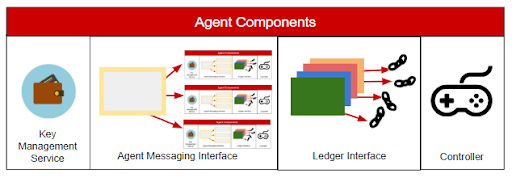
\includegraphics[width=0.7\linewidth]{images/Agent_Components.png}
    \caption[Aries Agent Architecture]{Aries Agent Architecture\protect \footnotemark}
    \label{fig:aries_agent_architecture}
\end{figure}

\footnotetext{\url{https://courses.edx.org/assets/courseware/v1/acc3247dbf74b710586a75f0854699ab/asset-v1:LinuxFoundationX+LFS172x+3T2019+type\@asset+block/Agent_Components.png}}

For this project the agents that will be used are the \acrfull{ACA-Py} implementation. According to the development team, "\textit{ACA-Py is built on the Aries concepts and features that make up Aries Interop Profile (AIP) 1.0, as well as many of the protocols that will be in AIP 2.0. ACA-Py’s supported Aries protocols include, most importantly, protocols for issuing, verifying, and holding VCs that work with a Hyperledger Indy distributed ledger and the Indy "AnonCreds" credential format. Contributors are actively working on adding support for other ToIP Layer 1 DID Utilities, and for other VC formats.}"\footnote{\url{https://github.com/hyperledger/aries-cloudagent-python}}.
At the time of writing, the project has a very active community with constant updates and implementation of Aries \glspl{RFC} to accommodate to the standards adopted for SSI (whether Hyperledger standards or ones by W3C).

The ACA-Py agents expose a variety of \acrfull{REST} endpoints, that when hit, will spark an action that can range from connecting to another agent, issue a credential, revoke a credential, and many others. These are all documented when deploying an ACA-Py agent, presented using SwaggerUI\footnote{Software used to visualize and interact with the API’s resources - \url{https://swagger.io/tools/swagger-ui/}}, allowing for an easy way to interact with the agents and be mindful of the necessary parameters for specific actions (for example a credential object needs to be attached to the specific POST request for issuing a credential).

An important aspect to consider when thinking of selecting an agent implementation is whether it supports mediation or not. In the context of agents, mediation is needed in two scenarios: when agents are not guaranteed to be online 100\% of the time, or when the agents do not want to have their Public DIDs written to the ledger (for privacy reasons), which leaves them without an endpoint for other agents to connect to. In those events, there should be a mediator agent acting similar to an inbox for e-mail, that stores incoming messages and sends them as soon as the offline agent is back online, addressing the first scenario. 
When the mediated agent connects to other agents via a pairwise DID communication, the endpoint of the mediated agent will appear to the agent it connects to as the one from its mediator, resolving the second scenario.
Mediation is facilitated within the Hyperledger ACA-Py agent, making it a strong agent implementation regarding this aspect.
The mediator is never aware of the final recipient of the messages, nor about the content of the message, since onion routing is baked-in the current implementation of the agents, allowing the solution to benefit from higher privacy measures.

% \paragraph{Other Agent Implementations} An agent can be tailored for each solution, which means that for the literature that was consulted, for example Terzi et al. \cite{terzi2020securing}, a close-source agent was used in the different agents. This restricts the number of open-source components that can be used to create an agent.

\paragraph{Decision}

Given the fact that the ACA-Py agent is at a stage where it can be used for the majority of actions regarding SSI (establish connections, issue and handle credentials, revocation, mediation, etc), is open-source and has a Ledger Interface compatible with Hyperledger Indy (the Distributed Ledger adopted as highlighted in Section~\ref{subsubsec:distributed_Ledger}), it will be the agent implementation used in the solution.

\subsubsection{Mobile Agent}
\label{subsubsec:mobile_agent}

At the time of writing there are several implementations for mobile agents (also mentioned as wallets), which are meant to be used by the individuals on their mobile devices. These offer an already defined logic for controlling the actions regarding handling connections to other agents and how to use verifiable credentials to verify proof requests. One limitation regarding mobile agents is that they do not have a specific endpoint for other agents to connect to. Instead they require an agent (which can be running in the cloud) to act as its mediator. Mediation is a mechanism which will be explained in Section~\ref{subsubsec:architecture_of_the_system}.

The current agents that support Self-Sovereign Identity, identified from literature and online research are: Lissi\footnote{\url{https://lissi.id/}}, eSatus\footnote{\url{https://esatus.com/}}, Trinsic\footnote{\url{https://trinsic.id/}} and Connect.me\footnote{\url{https://www.connect.me/}}. There is also the Aries Mobile Agent Xamarin\footnote{\url{https://github.com/hyperledger/aries-mobileagent-xamarin}} which is an open-source project hosted under Hyperledger ecosystem. 

Although in this case the Xamarin agent would be a solution within the same ecosystem (Hyperledger), it is not yet mature enough for testing, while the Trinsic Wallet agent offers a ready-to-use solution, that has the possibility to connect to any Hyperledger Indy Network. This last statement indicates that this agent implementation complies with the choice for the selected network (BCovrin Test Indy Network), which has been adopted following the reasons mentioned in Section~\ref{subsubsec:distributed_Ledger}. Additionally, the Trinsic Wallet agent offers under-the-hood support for mediation, satisfying a privacy concern that will be described ahead.

\paragraph{Decision}

For the reasons mentioned in this section, the Trinsic Wallet App has been adopted as part of the proposed solution for the Mobile Agents' implementation.

\subsection{Architecture for SSI with IoT}
\label{subsec:architecture_for_ssi_with_iot}

In this section an overview of a generic solution for a system which uses SSI applied to IoT devices is presented. In Figure~\ref{fig:general_architecture_ssi_with_iot} a diagram illustrates the solution which is generic and highlights the necessary components for a system which has: 
\begin{itemize}
    \item Enterprise agents (presented in \textcolor{blue}{\textbf{blue}} on the left side as Entity A, B and C); 
    \item Mobile agents (in \textcolor{red}{\textbf{red}}) and its need for a mediator agent (in \textcolor{purple}{\textbf{purple}});
    \item IoT devices which are resource constrained (in need of a static agent);
    \item IoT devices that are not resource constrained.
\end{itemize}

In a general solution designed for SSI with IoT, the necessary components are:

\begin{itemize}
    \item A Distributed Ledger to store the DID registry, schemas, credential definitions and revocation registries, as mentioned in Section~\ref{subsec:what_information_goes_onto_the_DLT?};
    \item Agents running on behalf of each entity with pre-configured logic on how to interact between each other;
    \item For the logic of which actions are to be performed by the agents it is necessary to have a controller which will vary depending on the given use case;
    \item It is also possible that the agents have a webpage running in front of the controller, which provides a User Interface (UI) to manage interactions with the agent.
\end{itemize}

In the diagram represented in Figure~\ref{fig:general_architecture_ssi_with_iot} there are three different types of agents which have already been discussed in Section~\ref{subsubsec:wallets_and_agents}, \ref{subsubsec:agent_technology} and \ref{subsubsec:mobile_agent}. There are the Edge and Cloud agents as well as the Mobile agents. 

A point worth reflecting on in this section is the fact that some agents should not have a public DID available in the ledger (for example the agents that represent individuals or IoT devices). In these events, the mediator is necessary to provide a routing path between these agents and the outside world. 
The Mobile Agent will need the mediator agent as mentioned previously, with said mediator running in the cloud. 
This mediation is also observed in Figure~\ref{fig:general_architecture_ssi_with_iot} since there are mediators present for the Resource-Constrained IoT devices as well as Private-Non-Resource IoT devices.



\begin{figure}[!htb]
    \centering
    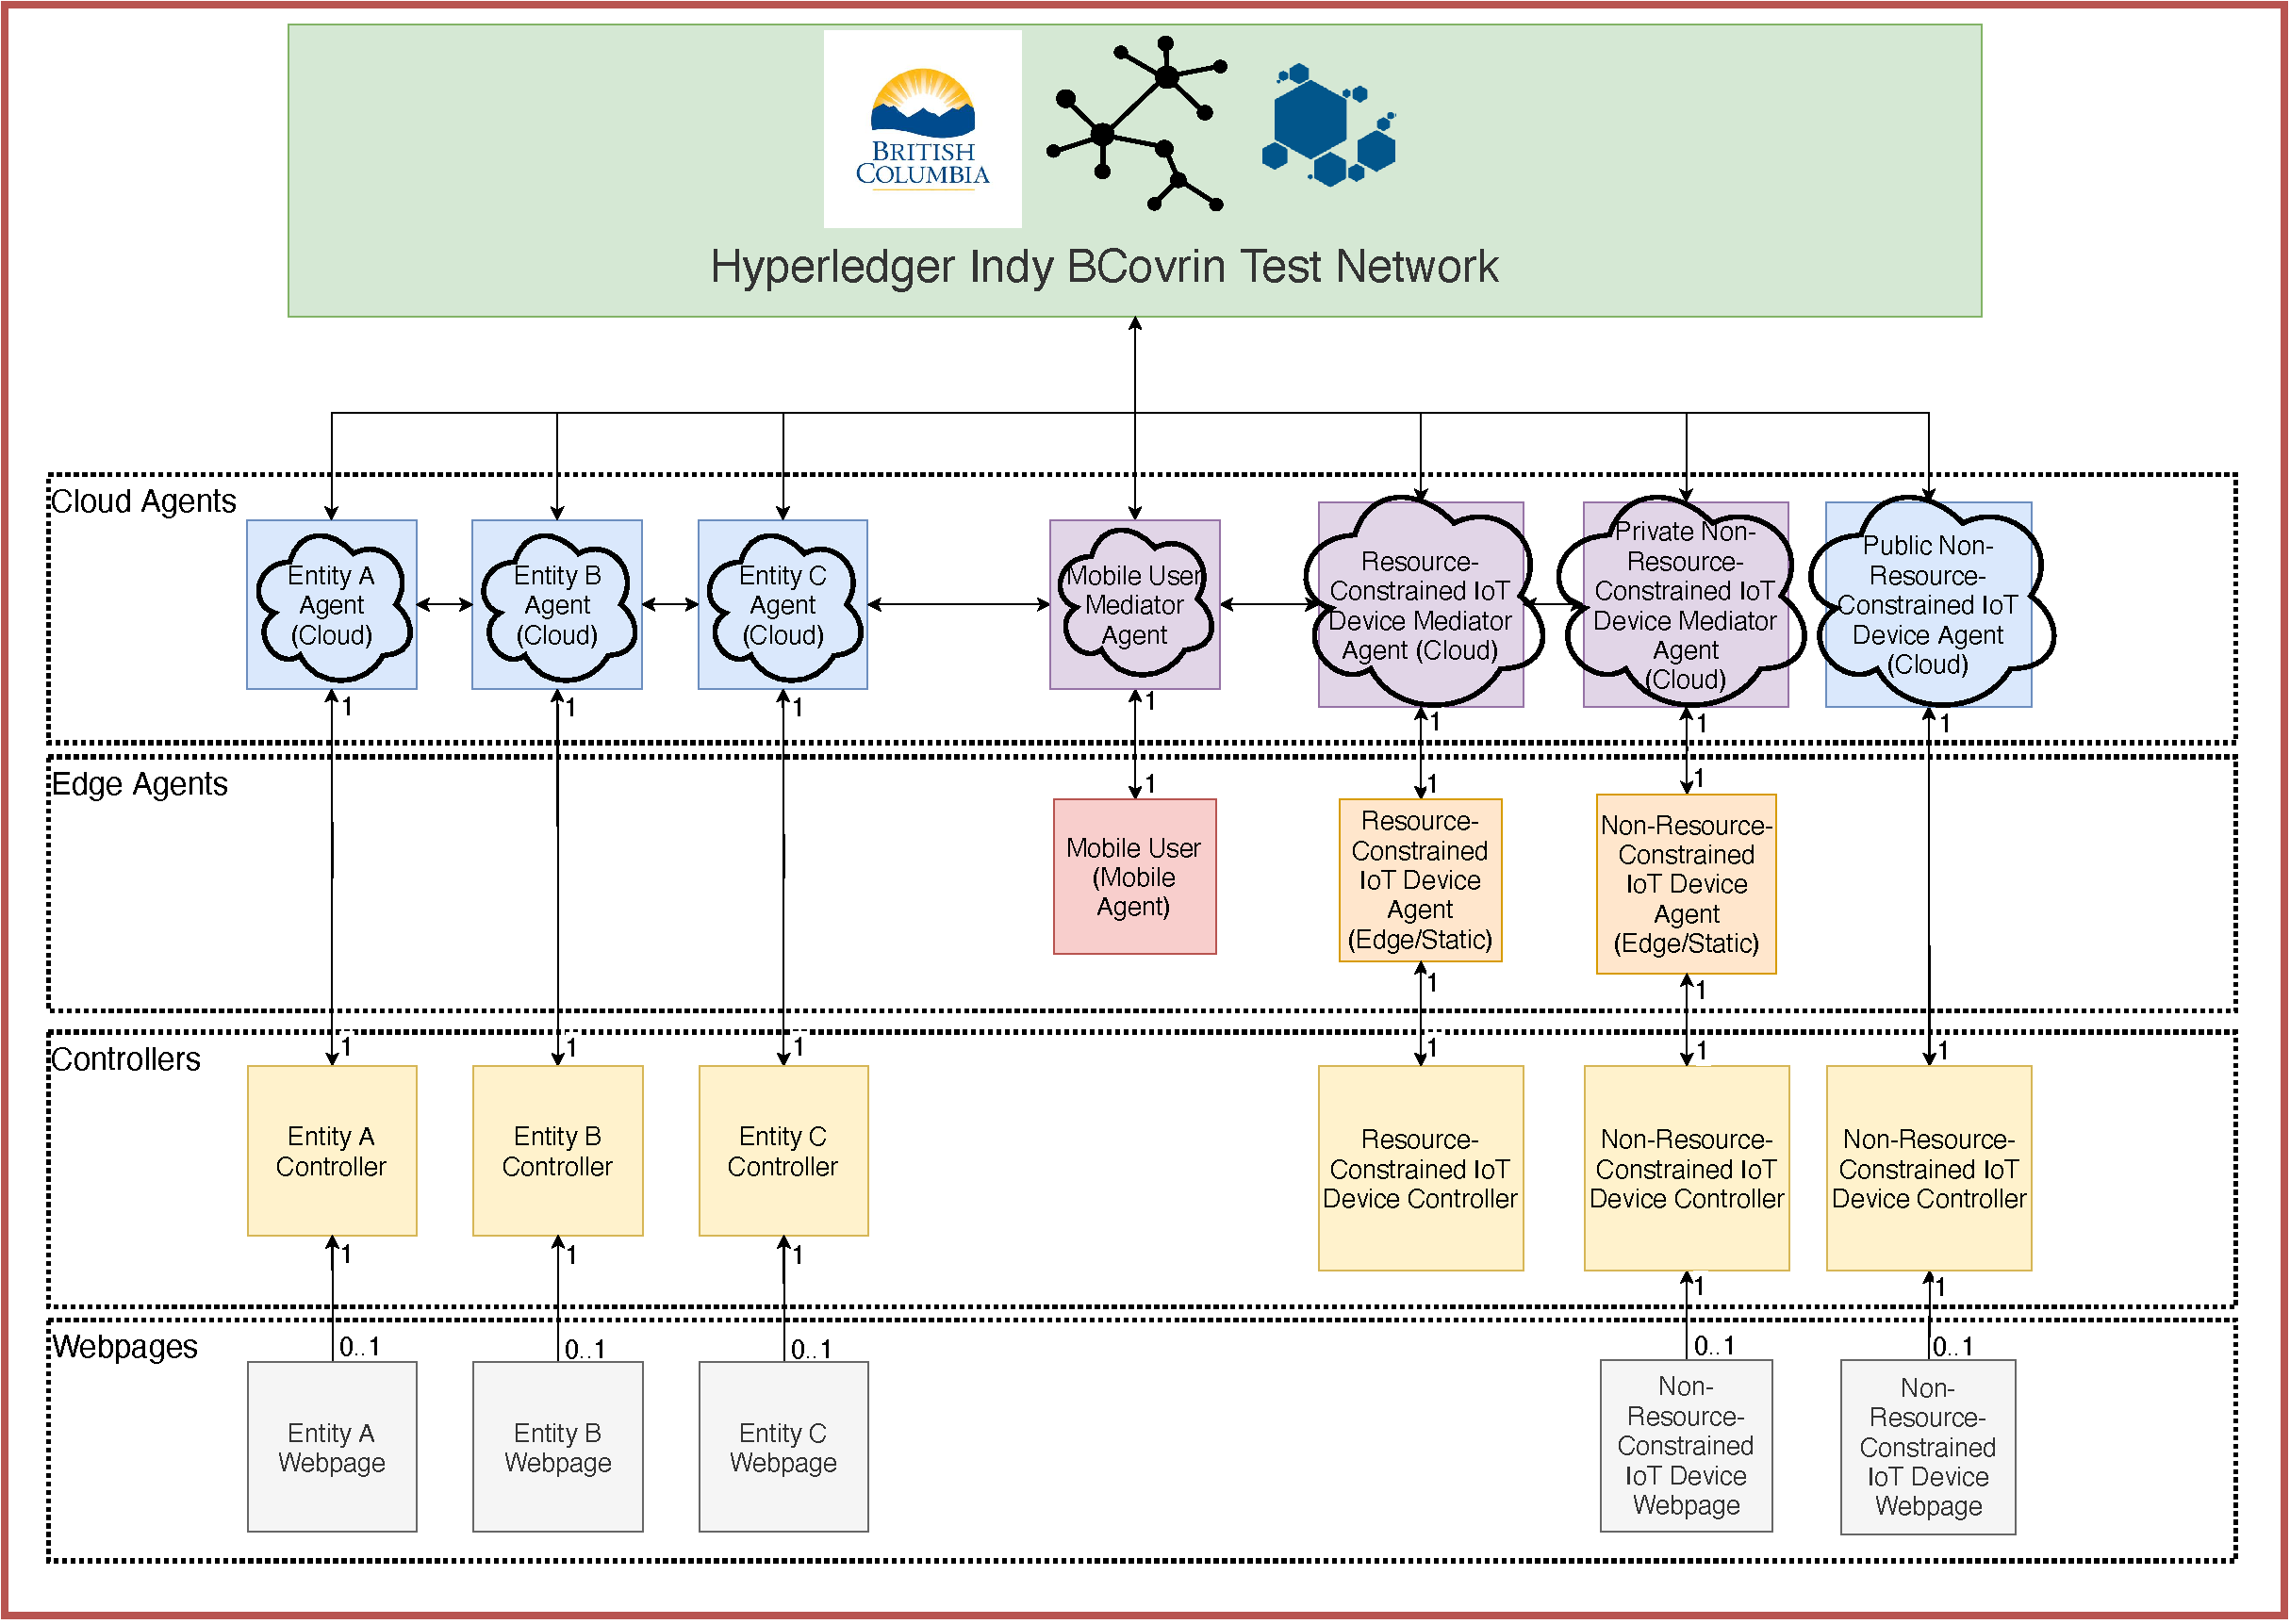
\includegraphics[width=0.85\linewidth]{images/SSIWithIoTArchitecture.pdf}
    \caption{General Architecture for SSI with IoT}
    \label{fig:general_architecture_ssi_with_iot}
\end{figure}

\newpage

\subsection{Electric Vehicle Charging System with SSI}
\label{subsec:architecture_for_electric_vehicle_charging_system_with_ssi}

For the design of the system to-be, the idea is to port the core concepts of the architecture presented in the general SSI with IoT design in Section~\ref{subsec:architecture_for_ssi_with_iot} into the architecture of the Electric Vehicle Charging System. This has to be done while still having in mind the core functionality for authentication of users and vehicles on this system, as presented earlier in Section~\ref{subsec:case_description}.

In this section a run-down of the flow of the system and its components will be presented, with focus on the interactions made between the agents, the different assumptions made, as well as a rationale for the decisions taken that combined into the proposed architecture. This is explained in detail in Section~\ref{subsubsec:architecture_of_the_system}. A detailed analysis on the mapping between real-life credentials and the Verifiable Credentials in the proposed architecture is made in Section~\ref{subsubsec:schemas_and_CDs}. The different flows present in this system and their specific use cases are illustrated in Section~\ref{subsubsec:information-flows-ssi}. A brief description of how each flow is ported to the new system is made. Additionally, for each use case description the agent interactions are highlighted with the appropriate level of detail, describing each party's role in the communication and the different assumptions made.

\begin{figure}[!htb]
    \centering
    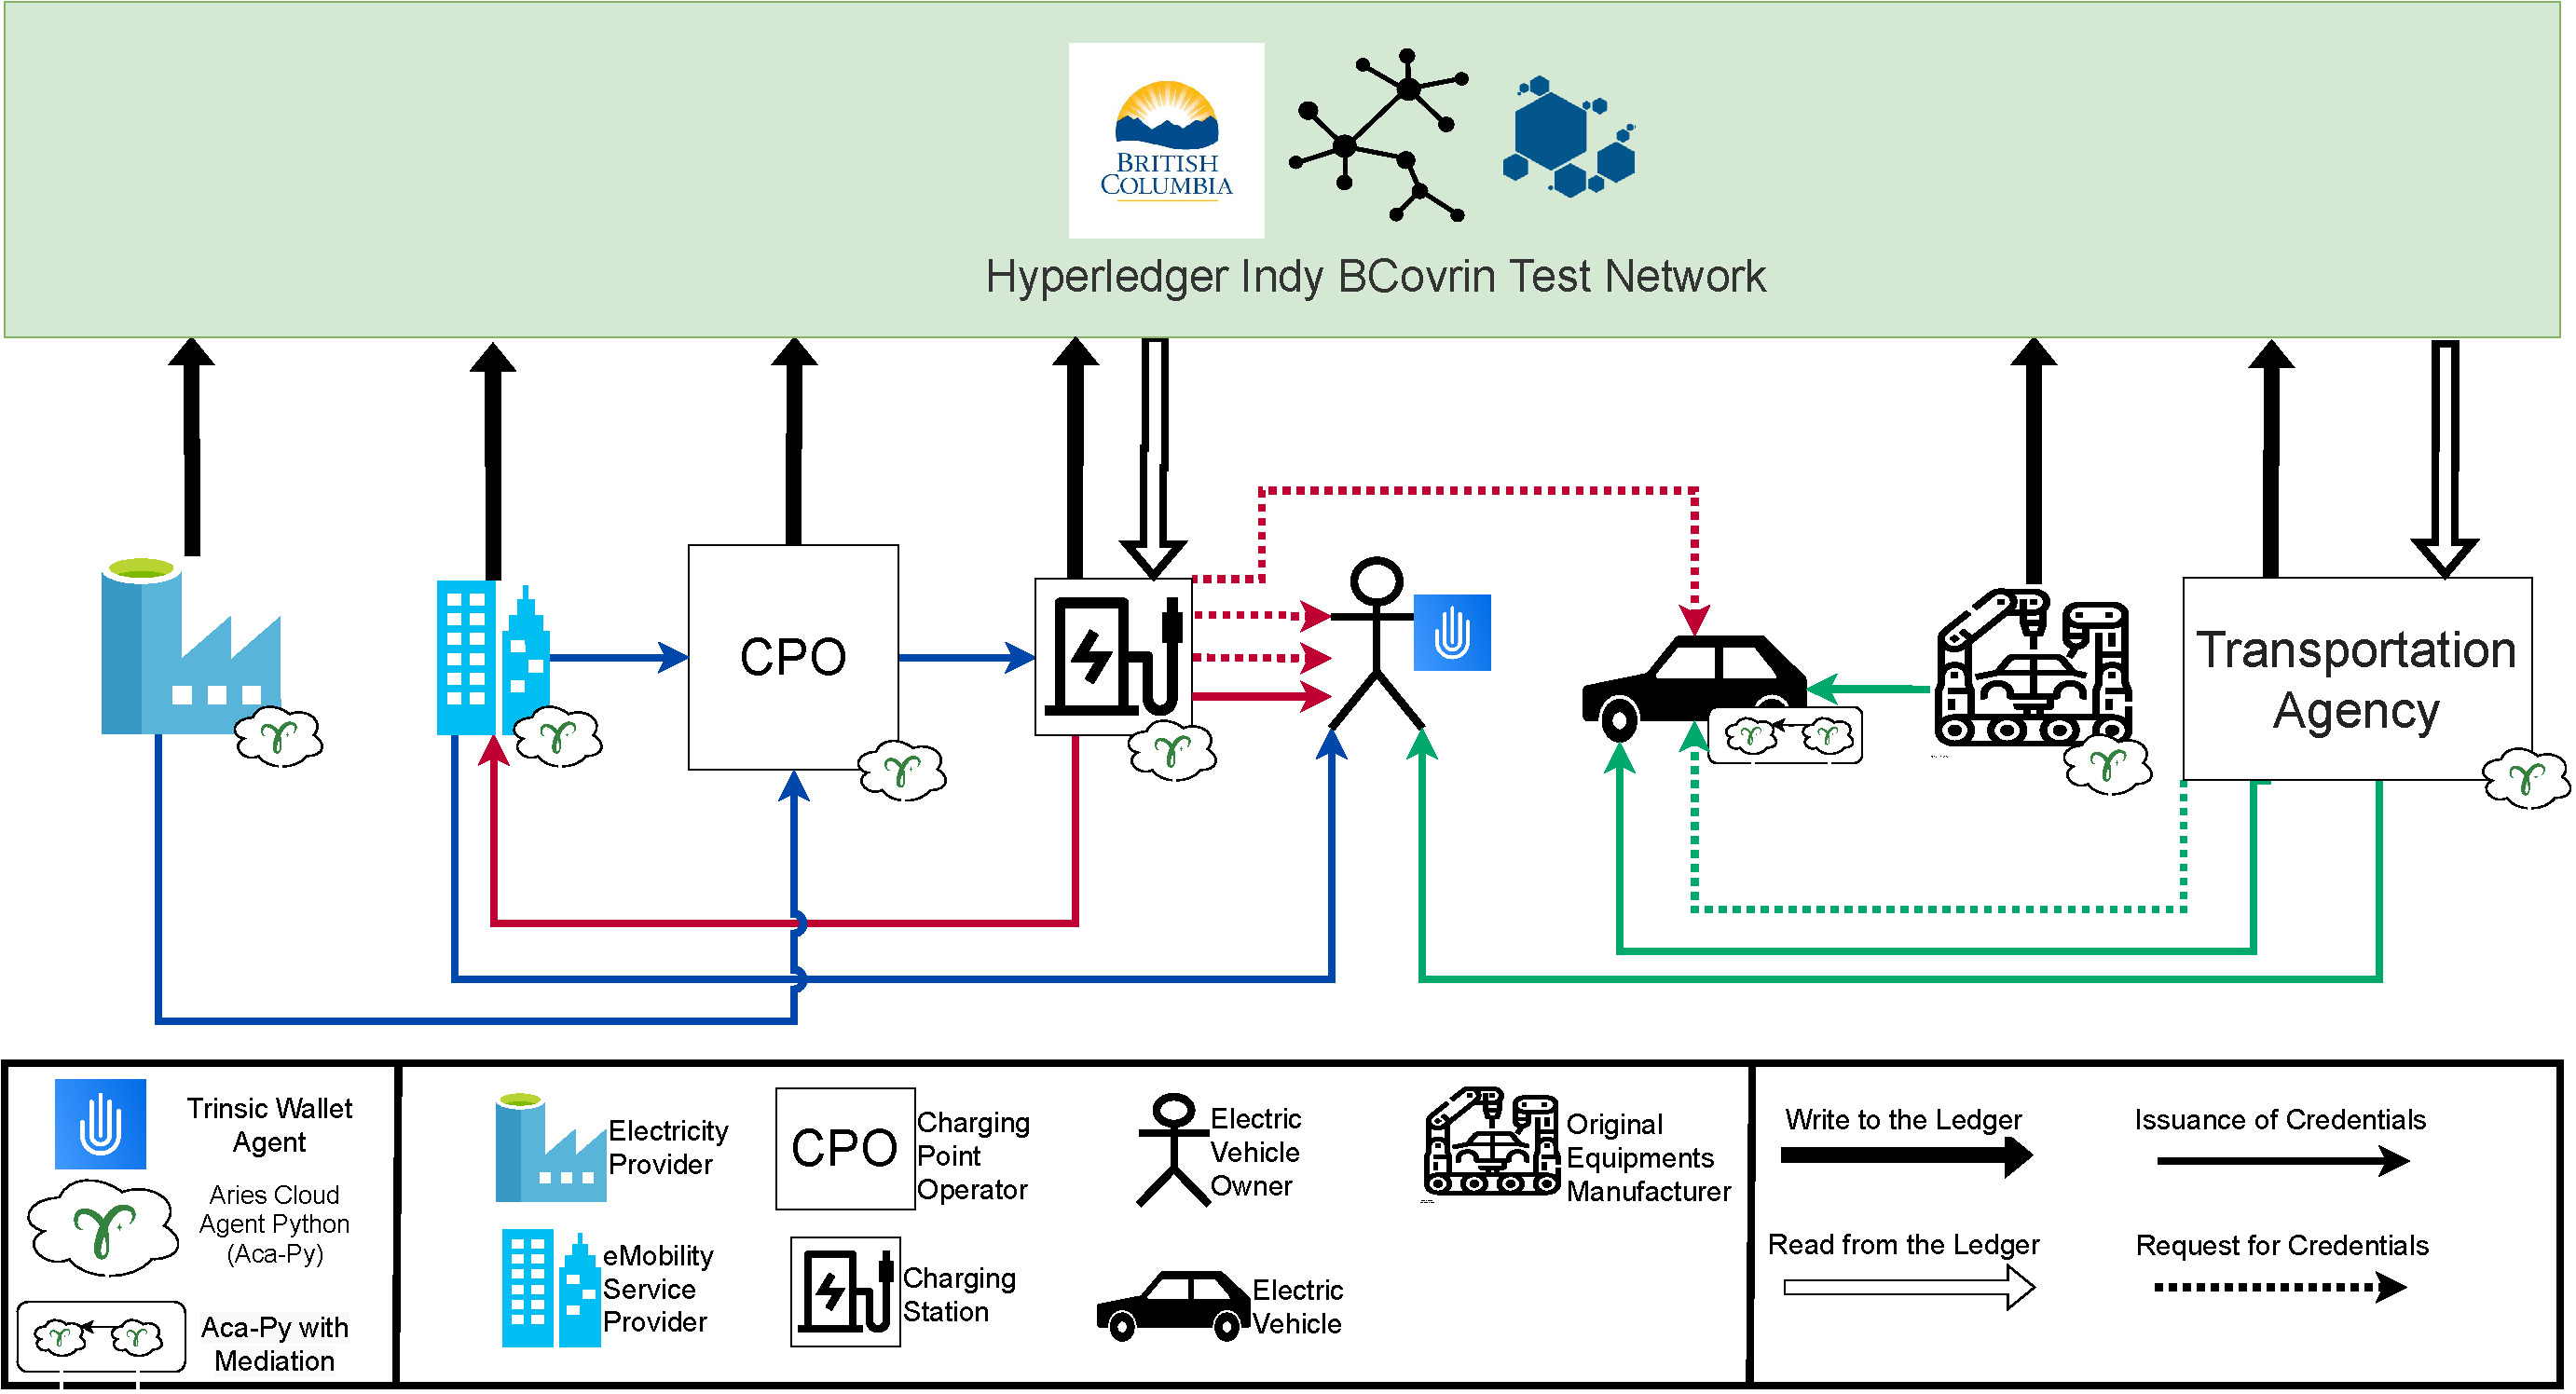
\includegraphics[width=\linewidth]{images/PaperHighLevelArchitecture.pdf}
    \caption{High-Level Architecture Electric Vehicle Charging System with SSI}
    \label{fig:High-Level_Architecture_SSI}
\end{figure}

\subsubsection{Architecture of the System}
\label{subsubsec:architecture_of_the_system}

In Figure~\ref{fig:High-Level_Architecture_SSI} a high-level architecture diagram of the Electric Vehicle Charging System with SSI is demonstrated. This diagram highlights the interactions between each party and between the parties and the Hyperledger Indy Network.

\paragraph{Agents}

Adding Agents to the parties listed in Section~\ref{subsubsec:users_and_information_flows}, and also including the Indy Distributed Network which implements the DLT are the first steps to migrate to the new architecture.
Each party in this diagram represents a group of entities, which will have one agent each. For the sake of simplification, in the diagram presented in Figure~\ref{fig:High-Level_Architecture_SSI} only one of each entity is displayed. 

All parties except the EV Owner are bearers of an ACA-Py, following the choices made in Section~\ref{subsubsec:agent_technology}. All of these ACA-Py agents need to be registered to the network (listed in Section~\ref{subsubsec:distributed_Ledger}) in order to be successfully deployed/started.
Although all agents except the EV Owners are running the ACA-Py agent, they are not all configured the same.
The EV is considered to be an entity whose identity and details should remain anonymous, similarly to the EV Owner. In these two instances (the EV and EV Owner) no public DIDs should be written to the ledger, in order to preserve privacy. 
In the case of the EV running the ACA-Py agent, the difference from the other parties is that no Public DID is registered to the network, and that way no other agent on the ledger will know how to connect to this EVs agent.

The EV Owner's agent is meant to be used as a personal device agent, hence the usage of the Trinsic Wallet Mobile App (available on the App Store and Google Play Store). This agent offers an easy-to-deploy scenario for users, without the need for any additional configurations on the developer or end-user end. This agent, as mentioned previously, is allowed to interact with the BCovrin Test Network without a Public DID. This allows for greater privacy since no details are written onto the ledger.

Following the introduction of the ACA-Py agents in Section~\ref{subsubsec:agent_technology}, and in order to provide a better understanding of the capabilities of the agents and how these can be used independently of the use case, an example of how to use the primary REST endpoints exposed by the agent implementation is presented below. 
In order for an entity agent to issue a credential to another agent, it is first necessary to create a \textit{credentialJSON} object following the specification provided in the agents documentation, and then perform a POST request to the agents endpoint using the following format:

\begin{lstlisting}[language=Bash]
    curl -XPOST -H "Content-type: application/json" -d '{credentialJSON}' 'issuerAgentEndpoint/issue-credential/send'
\end{lstlisting}

Since the implementation of the proposed solution makes use of the automation offered by the agents (by tweaking the deployment parameters, explained later in the deployment chapter), the flow of issuing a credential from one agent to another is automated after the first POST call is made (marked in the above snippet of the script as 'issuerAgentEndpoint/issue-credential/send'). Therefore, none of the other REST endpoints regarding accepting the credential or storing it in the entities' wallet is needed as this is done automatically by the agents.

\paragraph{Mediation}

Given that the EV and the EV Owners agents should not have public DIDs and therefore do not have endpoints to connect to, brings the need for mediation in the proposed solution, a term already introduced in Section~\ref{subsubsec:agent_technology}. 

For the EV agent mediation, another ACA-Py agent is deployed whose purpose is to act solely as a mediator for one EV agent. This mediation can be established during the deployment of each EV agent. Mediation is already implemented under-the-hood for the EV Owner, running the Trinsic Wallet agent, given that the latter handles mediation internally. 

This way, the connections established between the EV Owner/EV and their respective mediators, as well as the mediators with all other agents is end-to-end encrypted, preserving the privacy of the EV Owner and EV and allows them to receive messages later, if offline.

\paragraph{Network Roles and fees}

Given that the proposed solution uses a test network, there are no costs related to performing any actions. But, in a production environment, writing information to the ledger may cost money (for example Sovrin charges \$50 to write a Schema\footnote{\url{https://sovrin.org/issue-credentials/}} to its production network). In Figure~\ref{fig:High-Level_Architecture_SSI} this information regarding who writes to the ledger is marked with the lines going to the Hyperledger Indy BCovrin Test Network, which essentially marks the entities that in a production level network would need to pay fees.

\paragraph{Distributed Ledger}

The Distributed Ledger is responsible for storing the Public DIDs of issuing or mediator agents, and information regarding the schemas and credential definitions. Additionally it contains information about the revocation registries, so that revocation can be allowed in this system.
Every time an agent wishes to issue a new credential type to another agent, it needs to hold a credential definition previously written to the ledger, stating that it can issue credentials to others under a set of attributes defined in a linked schema (this schema may be issued by the same agent or a different one). From that point on, that agent is authorized to issue credentials under that credential definition.

\paragraph{Revocation Registry}

The revocation registry is used as a means to provide revocation to the credentials. It is not inherently included in the deployed network, but it is a component whose purpose is relevant together with an Hyperledger Indy network, hence this was abstracted in Figure~\ref{fig:High-Level_Architecture_SSI} and included it in the "Hyperledger Indy BCovrin Test Network". When a credential definition is created, and when the revocation flag is set to \textit{true}, a revocation registry will automatically be created, and a tails file will be uploaded to the revocation registry (also named as tails server). Revoking credentials is made the same way as issuing a credential, in the way that these actions are handled by the agents by means of REST APIs. When an agent wishes to revoke a credential that was previously issued, it adds a revocation registry entry to the tails server indicating the revocation of a given credential, so that verifiers can look up the credential on the tails server and validate whether the credential is still valid.

\subsubsection{Schemas and Credential Definitions}
\label{subsubsec:schemas_and_CDs}

One of the main goals of transposing the architecture of the current paper-based model to the SSI-powered system is to port credentials into VCs. These can be credentials that attest signed contracts, ownership attestations, legal documentation, etc. In this system there are a number of exclusive parties that will be allowed to create schemas and credential definitions, which will be used as the template to issue credentials to the remaining parties. After dissecting the problem and understanding where it is possible to create and adapt VCs, the following mapping listed in Table~\ref{tab:mapping_of_credentials} has been made.

\begin{table}[!htb]
    \begin{tabularx}{\linewidth}{|c|c|c|X|} 
    \hline
    \textbf{Credential ID} & \textbf{Schema and CD Issuers} & \textbf{Target Holders} & \textbf{Verbose} \\
            \hline
            1 & OEM & EV & Credential containing information on the EVs' VIN. \\
            \hline
            2 & TA & EV & Credential attesting the EV is registered and allowed to be driven on the streets. \\
            \hline
            3 & TA& EV Owner & Credential attesting that the EV Owner is allowed to drive the EV they possess. \\
            \hline 
            4 & eMSP & EV Owner & Credential representing signed contract between eMSP and EV Owner. \\
            \hline
            5 & eMSP & CPO & Credential representing signed contract between eMSP and CPO. \\
            \hline
            6 & CPO & CS & Credential attesting that a specific CS is owned by the respective CPO. \\
            \hline
            7 & CS & EV Owner \& eMSP & Credential containing receipt of charging transaction. \\
            \hline
            8 & EP & CPO & Credential representing signed contract between EP and CPO. \\
            \hline
    \end{tabularx}
    * For the sake of the proposed solution, the issuers of the schemas are the parties who issue said credentials. In a production environment these schemas can be issued by Governmental Parties or Domain-Regulatory Parties, in order to ensure interoperability between all the different vendors.
    \caption{Mapping of Paper-Based Credentials to Verifiable Credentials}
    \label{tab:mapping_of_credentials}
\end{table}

The attributes of the most important credentials in Table~\ref{tab:mapping_of_credentials} are listed below. More fields can be added to the credentials, allowing these to be used for other use cases and applications.

\begin{itemize}
    \item \textbf{Credential 1}
    \begin{itemize}
        \item VIN - The VIN number is used by the TA in order to validate that the EV is registered with a valid number by the OEM.
    \end{itemize}
    \item \textbf{Credential 2 and 3}
    \begin{itemize}
        \item registrationID - This registrationID is the link between the EV and its EVOwner, since both hold the same registrationID.
    \end{itemize}
    \item \textbf{Credential 4}
    \begin{itemize}
        \item eMSPcontractID - This contractID is used in the charging process as an identifier of the EVOwner to a contract that is valid, provided by the eMSP.
    \end{itemize}
    \item \textbf{Credential 7}
    \begin{itemize}
        \item kWh - This attribute holds the information regarding the price per kWh at the time of charging.
        \item Price - This attribute holds the information regarding the price of the charging transaction.
        \item eMSPContractID - This attribute is used to link transactions to a specific eMSPContractID (Credential 4).
    \end{itemize}
\end{itemize}

\subsubsection{Information Flows with SSI}
\label{subsubsec:information-flows-ssi}

In this section the different flows highlighted in Section~\ref{subsec:case_description} and how they are handled in the new system will be discussed, marking the similarities between the previous architecture and the proposed architecture with SSI, while also explaining the state of the wallet of the agents after each flow.

\paragraph{Service Providers Flow with SSI}
\label{paragraph:service_providers_flows_with_ssi}

In order for the system to be operational for authentication of EV Owners and charging of the EVs, credentials \#4, \#5, \#6 and \#8 need to be present upon the systems initial configuration. In the original architecture, an EV Owner needs to hold a contract with an eMSP in order to be allowed to charge the EV, for example. Other details about each credential and their purpose will be explained in-depth with each use case description. During this flow, credentials will only be issued from one party to another without any previous credential verification (at least with the current assumptions made). It is important to mention that the interactions in Figure~\ref{fig:High-Level_Architecture_SSI} with the \textcolor{blue}{\textbf{Blue Lines}}, correspond to the information provided in the \textbf{Service Providers} flow in Section~\ref{subsubsec:users_and_information_flows}. 

Before making this analysis, there are a number of assumptions that need to be made:

\textit{The EVOwner has a contract signed with the respective eMSP and the details have been agreed on by both parties in the physical world.}

Table~\ref{tab:roles_of_service_providers} highlights the parties and their respective roles (Issuer, Holder, Verifier and/or Trusted Party) in this particular flow.

\begin{table}[H]
    \centering
    \begin{tabular}{|c|c|c|c|c|}
        \hline
        \backslashbox{Party}{Role} & Issuer & Holder & Verifier & Trusted Party \\\hline
        eMSP & \checkmark &  & & \\
        Charging Point Operator & \checkmark & \checkmark & & \\
        Charging Station & & \checkmark & & \\
        Electricity Provider & \checkmark & & & \\
        EV Owner & & \checkmark & & \\
        \hline
    \end{tabular}
    \caption{Roles of the parties involved in the "Service Providers Flow"}
    \label{tab:roles_of_service_providers}
\end{table}

In this flow, the steps of the communication are represented in the System Sequence Diagram in Figure~\ref{fig:service_providers_ssd}. Note that given that this flow incorporates four different use cases, that are not dependent on each other, these have been separated both in the figure as well as in the description below, but can be performed in no particular order.

\begin{itemize}
    \item Use Case "EVOwner/eMSP"
    \begin{enumerate}
        \item eMSP: The interaction between the eMSP and the EVOwner should begin by the eMSP generating a connection invitation in the form of a QR Code using the HTTP endpoints provided by the agent. 
        \item EVOwner: The user scans the QR Code using the Trinsic Wallet App, and accepts the connection invitation. After this point the two agents are connected via a pairwise-DID channel.
        \item eMSP: The eMSP will then proceed to issue a "Contract between eMSP and EVOwner" (Credential \#4) credential to the EVOwner.
    \end{enumerate}
    \item Use Case "eMSP/CPO"
    \begin{enumerate}
        \item eMSP: The eMSP agent will send out a connection request to the CPO agent.
        \item CPO: The CPO agent accepts the connection request and after this point the two agents are connected via a pairwise-DID channel.
        \item eMSP: The eMSP will issue a "Contract between eMSP and CPO" (Credential \#5) to the CPO agent.
    \end{enumerate}
    \item Use Case "EP/CPO"
    \begin{enumerate}
        \item EP: The EP agent will send out a connection request to the CPO agent.
        \item CPO: The CPO agent accepts the connection request and after this point the two agents are connected via a pairwise-DID channel.
        \item EP: The EP will issue a "Contract between EP and CPO" (Credential \#8) to the CPO agent. 
    \end{enumerate}
    \item Use Case "CPO/CS"
    \begin{enumerate}
        \item CPO: The CPO agent will send out a connection request to the CS agent.
        \item CS: The CS agent accepts the connection request and after this point the two agents are connected via a pairwise-DID channel.
        \item CPO: The CPO will issue a "Ownership of CS" (Credential \#6) to the CS agent. 
    \end{enumerate}
\end{itemize}

During the "Service Providers" flow the mentioned agents should receive the following credentials in their wallets:
\begin{itemize}
    \item EV Owner Agent Wallet
        \begin{enumerate}
            \item Credential (\#4) with Contract information with eMSP
        \end{enumerate} 
    \item CPO Agent Wallet
        \begin{enumerate}
            \item Credential (\#5) with Contract information with eMSP
            \item Credential (\#8) with Contract information with EP
        \end{enumerate}
    \item CS Agent Wallet 
        \begin{enumerate}
            \item Credential (\#6) with Proof of Ownership from CPO
        \end{enumerate}
\end{itemize}

\begin{figure}[!h]
    \centering
    \frame{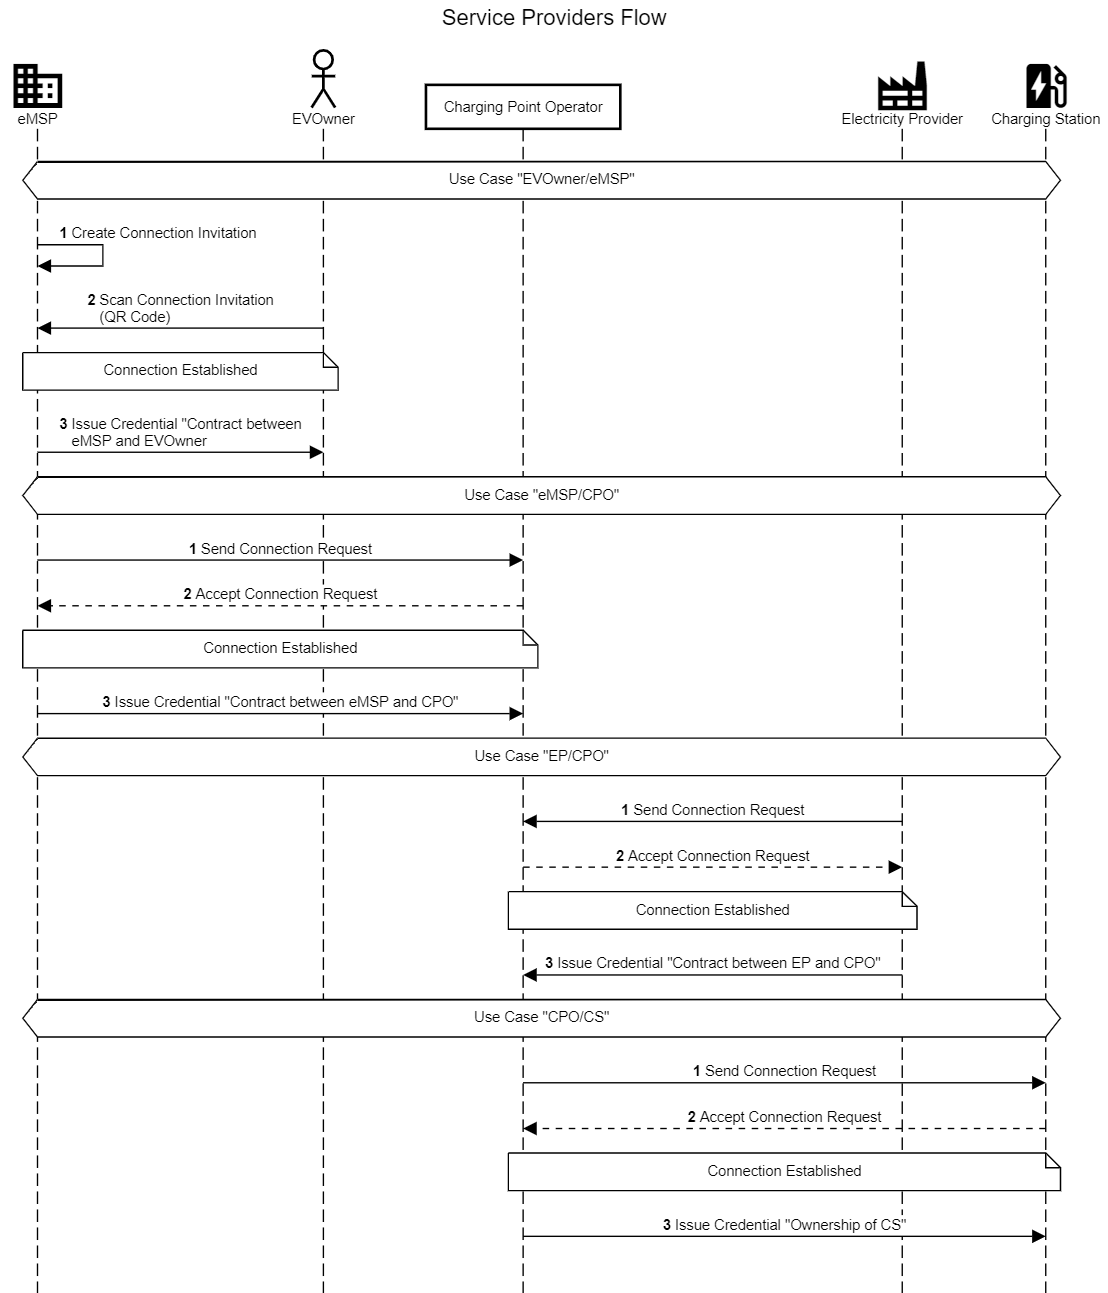
\includegraphics[keepaspectratio=true,width=0.85\textwidth]{images/SSDs/Service_Providers_Flow.png}}
    \caption{Service Providers Flow System Sequence Diagram}
    \label{fig:service_providers_ssd}
\end{figure}

\newpage

\paragraph{EV Owner and EV Interactions with SSI}
\label{paragraph:ev_owner_and_ev_interactions_with_ssi}

The \textbf{EV Owner and EV Interactions} flow is ported over to the new system with the usage of the interactions marked with the \textcolor{green}{\textbf{Green Lines}} in Figure~\ref{fig:High-Level_Architecture_SSI}. This is the first part of the system that requires credential verification. It starts with the EV being issued a VIN by the OEM through means of a credential. After that, the EV is meant to be registered by the local TA (for example the RDW in the Netherlands) and should be given a credential to attest this process. The EV Owner will need to confirm with the TA that it owns the EV it wishes to register; this could be perceived as a credential to add in the future to the system, so in order to simplify this portion of the system an assumption is made that the EV Owner is able to present a credential to this effect. After this, the TA issues a credential to the EV Owner with matching information that can link the EV Owner and its EV (for example the registration ID present in both credentials).

Before making this analysis, there are a number of assumptions that need to be made:
\begin{itemize}
    \item \textit{The OEM is the party that creates the vehicle, hence it can manually operate and deploy the EVs agent and establish a connection to it.}
    \item \textit{The EVOwner has a proof of purchase that is sent to the TA which entitles it to register the EV in their name.}
    \item \textit{The EV Owner and the EV will hold the same registration ID in their credentials given out by the TA, in order to link the two.}
\end{itemize}

Table~\ref{tab:roles_ev_and_ev_owner_interactions} highlights the parties and their respective roles (Issuer, Holder, Verifier and/or Trusted Party) in this particular part of the use case.

\begin{table}[H]
    \centering
    \begin{tabular}{|c|c|c|c|c|}
        \hline
        \backslashbox{Party}{Role} & Issuer & Holder & Verifier & Trusted Party \\\hline
        EV & & \checkmark & & \\
        EV Owner & & \checkmark & & \\
        TA & \checkmark & & \checkmark & \\
        OEM & \checkmark & & & \checkmark \\
        \hline
    \end{tabular}
    \caption{Roles of the parties involved in the "EV Registration and EV Ownership Registration" use case}
    \label{tab:roles_ev_and_ev_owner_interactions}
\end{table}

In this Information Flow, the steps of the communication are represented in the System Sequence Diagram in Figure~\ref{fig:ev_and_ev_owner_interactions_ssd}:

\begin{enumerate}
    \item EV: The flow commences with the EV sending a connection request (previously generated) to the OEM agent.
    \item OEM: The OEM receives the invitation and accepts it, establishing a pairwise-DID connection between the two agents.
    \item OEM: The OEM agent now issues a "Vehicle VIN" (Credential \#1) credential to the EV agent.
    \item EV: The EV agent now wishes to connect to the TA agent, sending a connection request to the latter.
    \item TA: The TA agent receives the connection request and accepts it, establishing a pairwise-DID connection between the two agents.
    \item TA: The TA agent now requests the "Vehicle VIN" credential from the EV, which was issued previously by the OEM (Credential \#1). It requests the VIN attribute and whether the expiration date is greater than the current date.
    \item EV: The EV receives the presentation request and generates a proof presentation using the credential issued by the OEM earlier.
    \item EV: The EV now sends the proof presentation to the TA agent.
    \item TA: The TA agent receives the proof, verifies it and proceeds to send an "EV Registration" (Credential \#2) credential to the EV.
    \item TA: The interaction between the TA and the EVOwner should begin by the TA generating a connection invitation in the form of a QR Code using the HTTP endpoints provided by the agent. 
    \item EVOwner: The user scans the QR Code using the Trinsic Wallet App, and accepts the connection invitation. After this point the two agents are connected via a pairwise-DID channel.
    \item TA: An event which is not contemplated in the PoC is the agent holding a credential to attest proof of purchase of the EV to register it. But in an ideal scenario the TA agent requests a "Proof of Purchase" credential from the EVOwner.
    \item EVOwner: The EVOwner receives the presentation request and generates a proof presentation with the "Proof of Purchase" credential (which is an assumption and is not contemplated in this PoC, as previously stated).
    \item EVOwner: The EVOwner now sends the proof presentation to the TA agent.
    \item TA: At last, the TA agent issues an "EV Owner Registration" (Credential \#3) credential to the EVOwner.
    
\end{enumerate}

\begin{figure}[!]
    \centering
    \frame{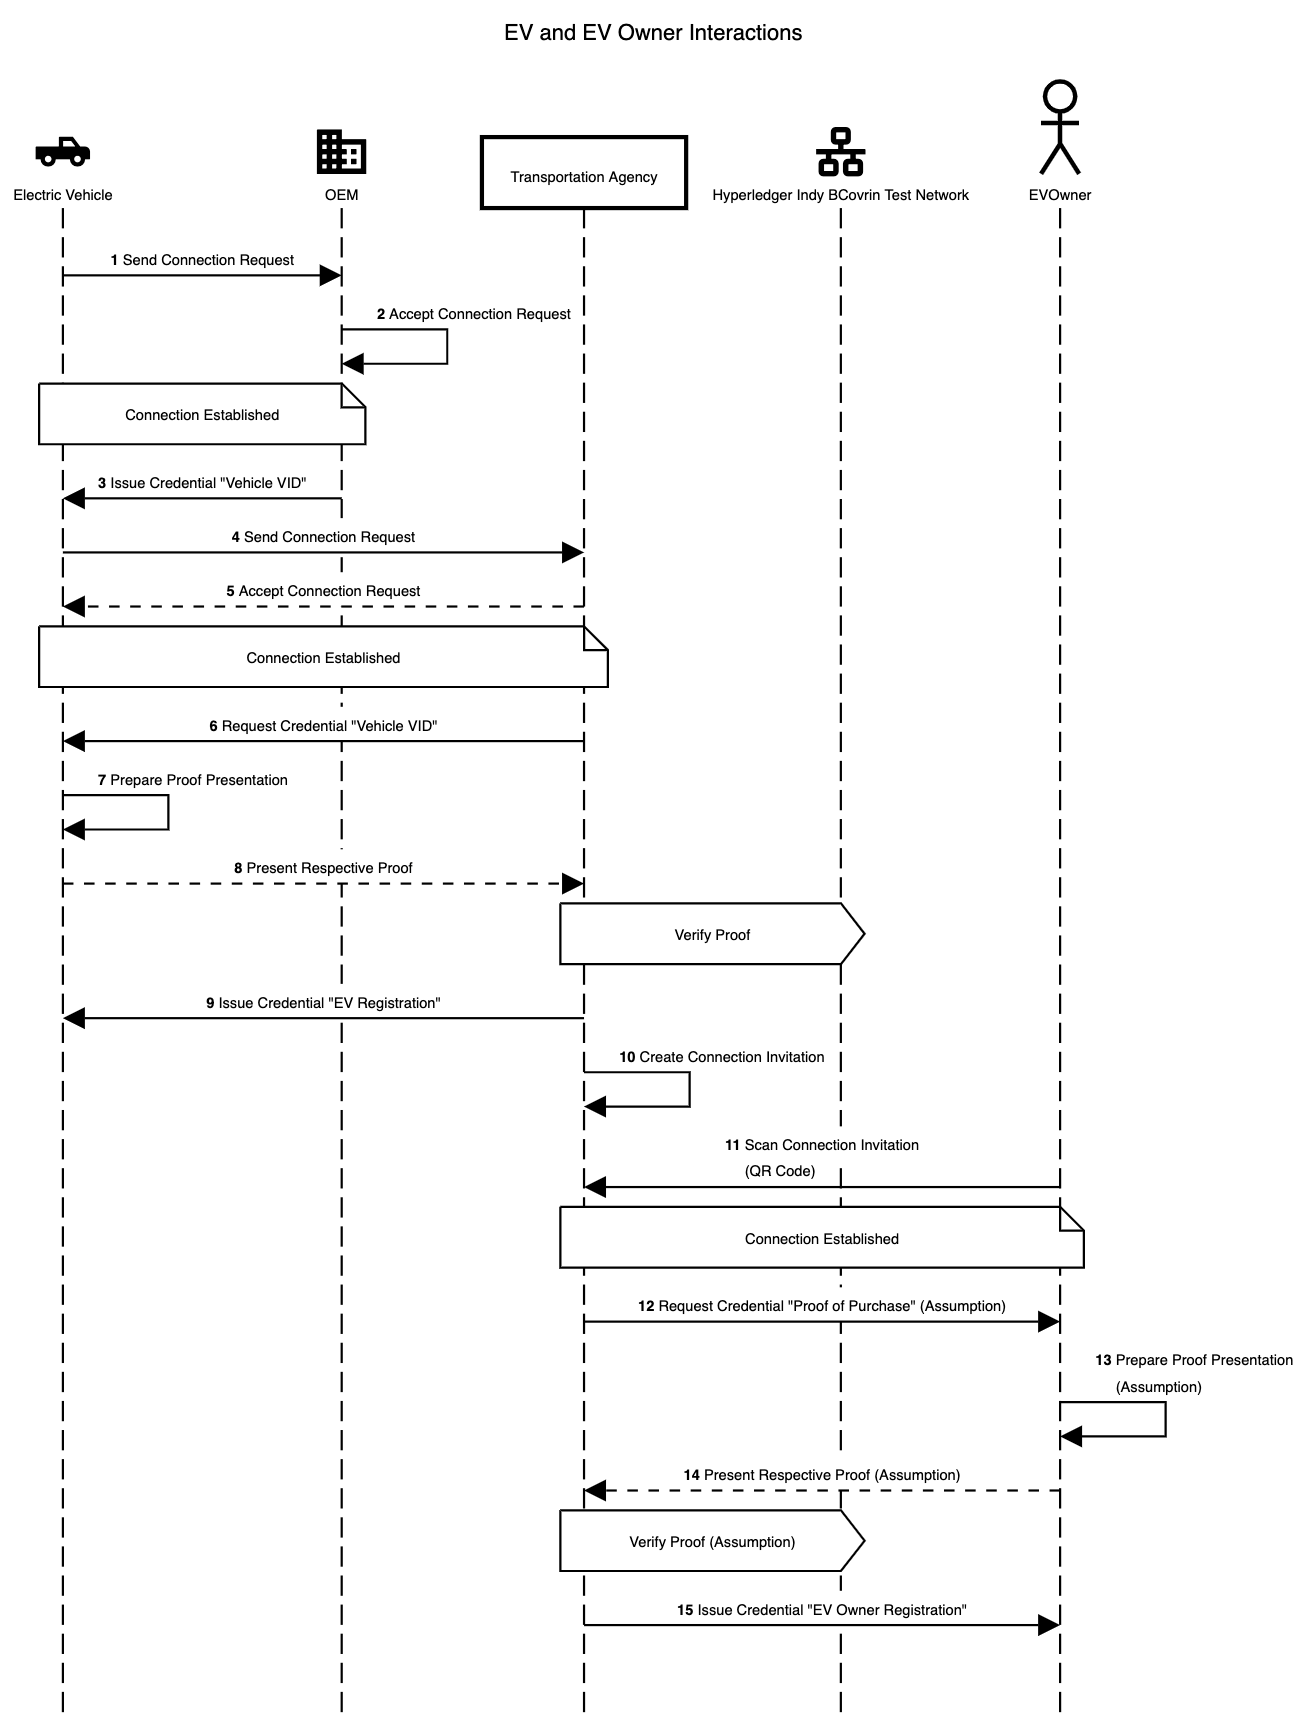
\includegraphics[keepaspectratio=true,width=\textwidth]{images/SSDs/EV_and_EV_Owner_Interactions.png}}
    \caption{EV and EV Owner Interactions System Sequence Diagram}
    \label{fig:ev_and_ev_owner_interactions_ssd}
\end{figure}

During the "EV Owner and EV Interactions" flow the mentioned agents should receive the following credentials in their wallets:

\begin{itemize}
    \item EV Agent Wallet
    \begin{enumerate}
        \item Credential (\#1) with Vehicle VIN from OEM
        \item Credential (\#2) with EV Registration from TA 
    \end{enumerate}
    \item EV Owner Agent Wallet 
    \begin{enumerate}
        \item Credential (\#3) with EV Owner Registration from TA
    \end{enumerate}
\end{itemize}

\paragraph{Charging and Billing Flow with SSI}
\label{paragraph:charging_and_billing_flow_with_ssi}

The most important part of this system is exactly demonstrating how to improve the privacy of the act of charging the EV; additionally, the system with SSI aims to tackle one of the key issues with the previous architecture: to provide means for the users to know the kWh rate, hence giving the opportunity to deny charging if the rate is too high according to the users desire. Additionally, it is also important to introduce in the system a way for the user to know how much they have spent after each charging session, and keep a record of that.
For this, the proposed architecture aims at the end of each transaction to give power to each Charging Station agent to issue a credential to the EV Owner with a "receipt-like" credential, that can be used later to prove claims and also to the eMSP to prove that a specific user has charged its vehicle (seen with the \textcolor{red}{\textbf{Red Lines}} in Figure~\ref{fig:High-Level_Architecture_SSI}). In order for EV Owners to know the rate at which the EV will be possibly charged, the Charging Station agent shall communicate with the CPO agent to obtain this information, and pass it on as a DIDComm Basic Message\footnote{\url{https://github.com/hyperledger/aries-rfcs/tree/527849ec3aa2a8fd47a7bb6c57f918ff8bcb5e8c/features/0095-basic-message}}.

Before making this analysis, there are a number of assumptions that need to be made:

\textit{The connection between the Charging Station and the EV is simplified since the process to send information from an EV to a CS falls out of the scope of this study. The reason is that the domain-specific protocols are not easy to integrate in this solution and need to be better assessed in the future.}

Table~\ref{tab:roles_of_charging_and_billing} highlights the parties and their respective roles (Issuer, Holder, Verifier and/or Trusted Party) in this particular part of the use case.

\begin{table}[H]
    \centering
    \begin{tabular}{|c|c|c|c|c|}
        \hline
        \backslashbox{Party}{Role} & Issuer & Holder & Verifier & Trusted Party \\\hline
        Charging Station & \checkmark & & \checkmark & \\
        EVOwner & & \checkmark & & \\
        Electric Vehicle & & \checkmark & & \\
        eMSP & & \checkmark & & \checkmark \\ 
        Transportation Agency & & & & \checkmark \\
        \hline
    \end{tabular}
    \caption{Roles of the parties involved in the "Charging and Billing Flow"}
    \label{tab:roles_of_charging_and_billing}
\end{table}

In this use case, the steps of the communication are represented in the System Sequence Diagram in Figure~\ref{fig:charging_and_billing_ssd}.

The steps are explained in detail in the following list:

\begin{enumerate}
    \item CS: The interaction should begin by the EV Owner arriving at a Charging Station, that will generate a connection invitation in the form of a QR Code using the HTTP endpoints provided by the agent. 
    \item EVOwner: The EVOwner scans the QR Code using the Trinsic Wallet App, and accepts the connection invitation. After this point the two agents are connected via a pairwise-DID channel.
    \item CS: The Charging Station agent will then request the credential attributes from the EVOwner that prove they hold a contract with an eMSP (Credential \#4).
    \item EVOwner: The EVOwner receives a credential presentation request on the Trinsic Wallet App, and assuming it agrees to disclose the information regarding "Contract ID", "eMSP Company Name" and use ZKP to prove that the "Expiration date of the contract" is greater than the current date, the Trinsic Wallet App will automatically fetch all the relevant attributes from the stored credentials and generate the proof.
    \item EVOwner: The Trinsic Wallet App then submits this proof and sends it back to the CS agent, with a reference to the Credential Exchange ID created by the CS agent in Step 3.
    \item CS: The CS agent receives the proof and verifies it, checking the revocation status of the presentation.
    \item CS: The same process of Steps 3-6 is repeated for the credentials that attest the EV Ownership from the EVOwner, previously issued by the TA (Credential \#3).
    \item CS: In case the EVOwner has a valid contract with an eMSP, the CS will proceed to contact the CPO agent and request the price per kWh for a user contracted under that eMSP, since this can vary depending the contracts signed between the CPOs and the eMSPs. Otherwise the charging session is rejected.
    \item CPO: The CPO agent will receive the message from the CS agent and reply accordingly with a charging rate.
    \item CS: The CS will receive the message and present this information to the EVOwner on the CS dashboard.
    \item CS: The CS will now connect to the EV in order to compare the credential attributes from the EV Owner and the EV and validate they are indeed linked.
    \item EV: The EV agent will accept the connection request from the CS (Note that this process is an assumption and needs to be studied in depth in the future work).
    \item CS: The same process of Steps 3-6 is repeated for the credentials that attest the EV Registration coming from the EV, issued by the TA (Credential \#2).
    \item CS: The values presented by both the EV and EVOwner are compared, and if they match, the charging session starts. Otherwise the charging session is rejected.
    \item CS: At the end of the charging session the CS issues a credential to the EVOwner and the respective eMSP with a receipt of the charging session (Credential \#7).
\end{enumerate}

\begin{figure}[!]
    \centering
    \frame{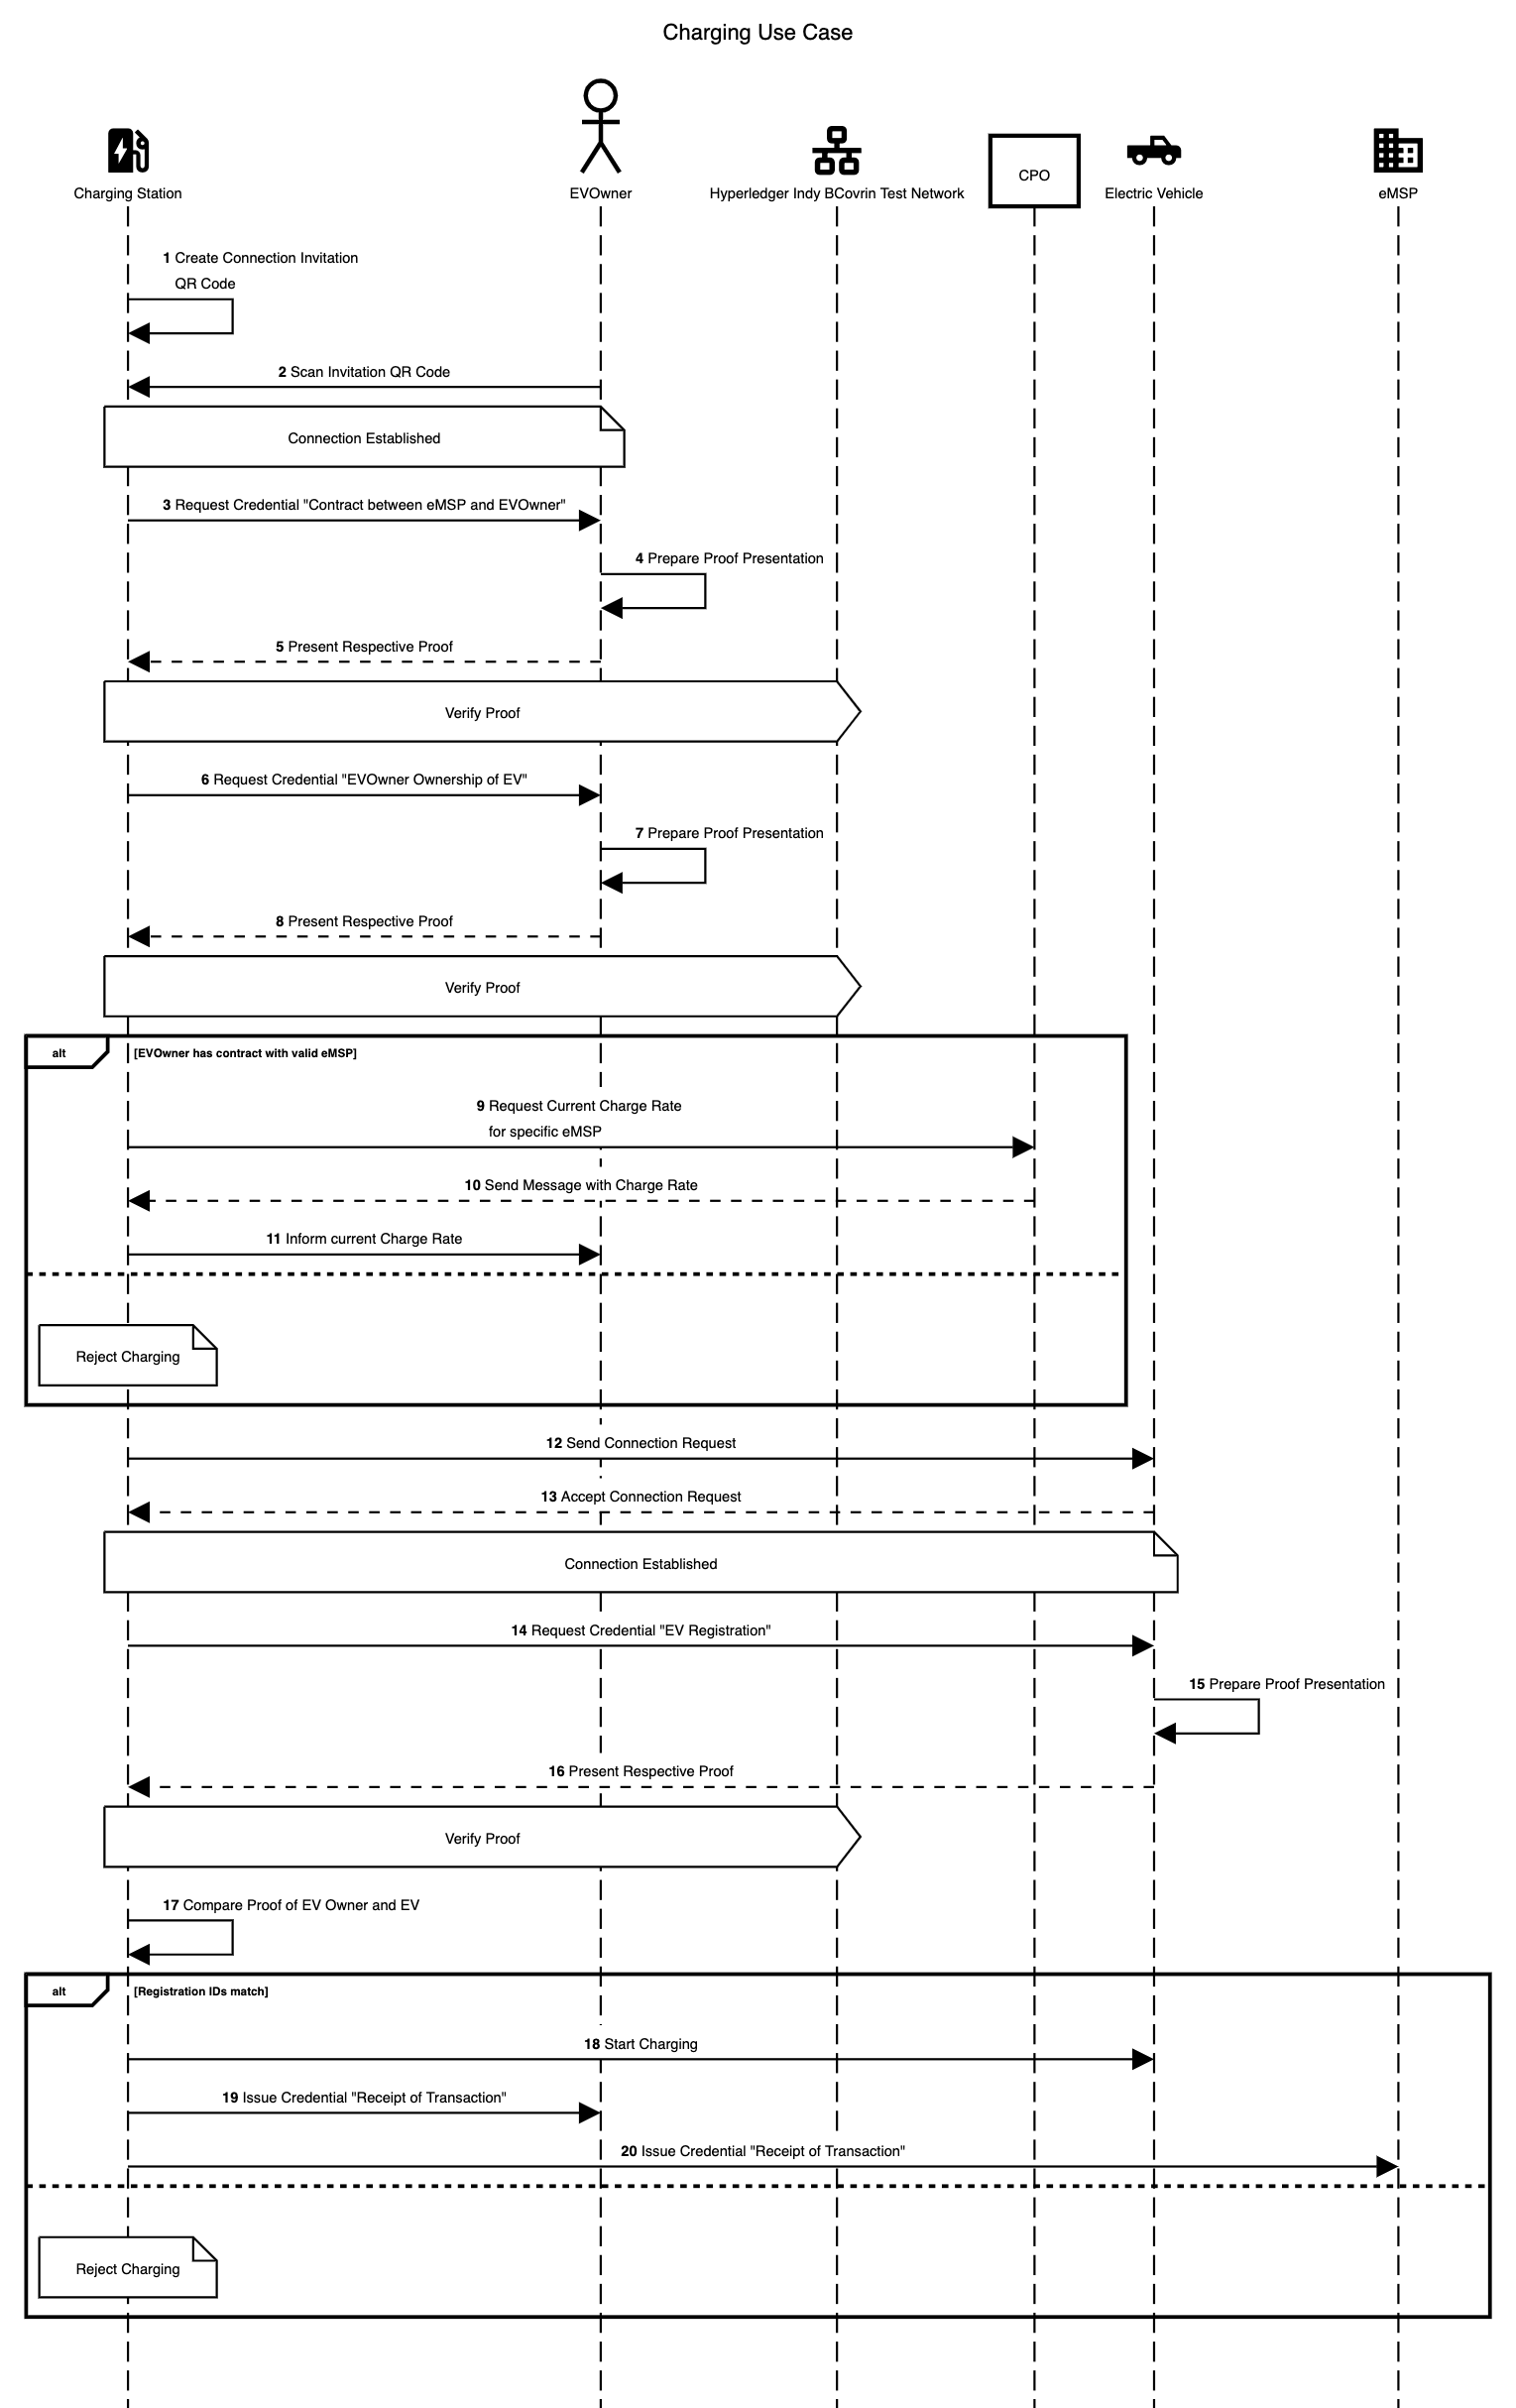
\includegraphics[keepaspectratio=true,height=\textheight]{images/SSDs/Charging_SSD.png}}
    \caption{Charging and Billing Use Case System Sequence Diagram}
    \label{fig:charging_and_billing_ssd}
\end{figure}


During the "Charging and Billing" flow the mentioned agents should receive the following credentials in their wallets:

\begin{itemize}
    \item EV Owner Agent Wallet
    \begin{enumerate}
        \item Credential (\#7) with Receipt of Charging Session from Charging Station
    \end{enumerate}
    \item eMSP Agent Wallet
    \begin{enumerate}
        \item Credential (\#7) with Receipt of Charging Session from Charging Station
    \end{enumerate}
\end{itemize}


\section{Implementation and Deployment}
\label{sec:implementation_and_deployment_details}

In this chapter the implementation details for a proof-of-concept prototype of the proposed solution, as well as the deployment procedures for it are discussed, with in-depth explanations of the components of the system and the responsibilities of each script. The source code discussed here can be found in a GitHub repository\footnote{\url{https://github.ibm.com/Filipe-Capela-CIC-Netherlands/SSI-IoT-PoC}} with more comments on the structure of the source code.

A list of the software that was used for this implementation and their respective versions can be seen in Table~\ref{tab:list_of_software}.

\begin{table}[!htb]
    \centering
    \begin{tabularx}{\linewidth}{|c|c|X|}
    \hline
    \textbf{Software} & \textbf{Version} & \textbf{Repository} \\
    \hline
    Operating System & macOS Big Sur 11.3 & - \\
    Docker Engine & 20.10.5 & https://docs.docker.com/engine/install/ \\ 
    Tails Server & - & https://github.com/bcgov/indy-tails-server \\
    Aries Cloud Agent - Python  & 0.6.0 & https://github.com/hyperledger/aries-cloudagent-python \\ 
    Trinsic Wallet Agent & 3.2.1 & - \\
    pgrok & 3.2.0 & https://github.com/jerson/pgrok \\ 
    NestJS & 7.5.0 & https://github.com/nestjs/nest \\ 
    AngularJS & 12.0.4 & https://github.com/angular/angular \\ 
    \hline
    \end{tabularx}
    \caption{List of the utilized software, and respective versions and repositories}
    \label{tab:list_of_software}
\end{table}

\subsection{Implementation Details}
\label{subsec:implementation_details}

A number of components were needed to facilitate agent deployment, ledger tests and also software deployment. The system follows the structure presented in Section~\ref{subsec:architecture_for_ssi_with_iot}, where an Agent, a Controller and a Webpage are present for most of the different entities' agent. In Figure~\ref{fig:Implementation_Architecture} the prototypes' architecture is presented, with all the implemented components and how these communicate with each other. The agents can connect to each other through the DIDComm protocol (explained in Section~\ref{subsubsec:didcomm}). Whenever a REST endpoint is hit on the NodeJS backend, it triggers a REST call to the agents available endpoints (provided by the ACA-Py implementation) to perform specific actions (start a connection, issue a credential, request credential verification process, etc). The two agents in purple are special since they are acting as mediator agents for both the EVOwner and the EV agents, in red and orange respectively. The EVOwner agent and its mediator are provided by the Trinsic Wallet App, while the EV Mediator agent is an ACA-Py agent that is configured manually to act as a mediator. 
The Webpages for each of the agents interactions were created using the Angular Framework and provide means contact the backend or the agents directly and have them execute certain actions related to the use case.

\begin{figure}[!htb]
    \centering
    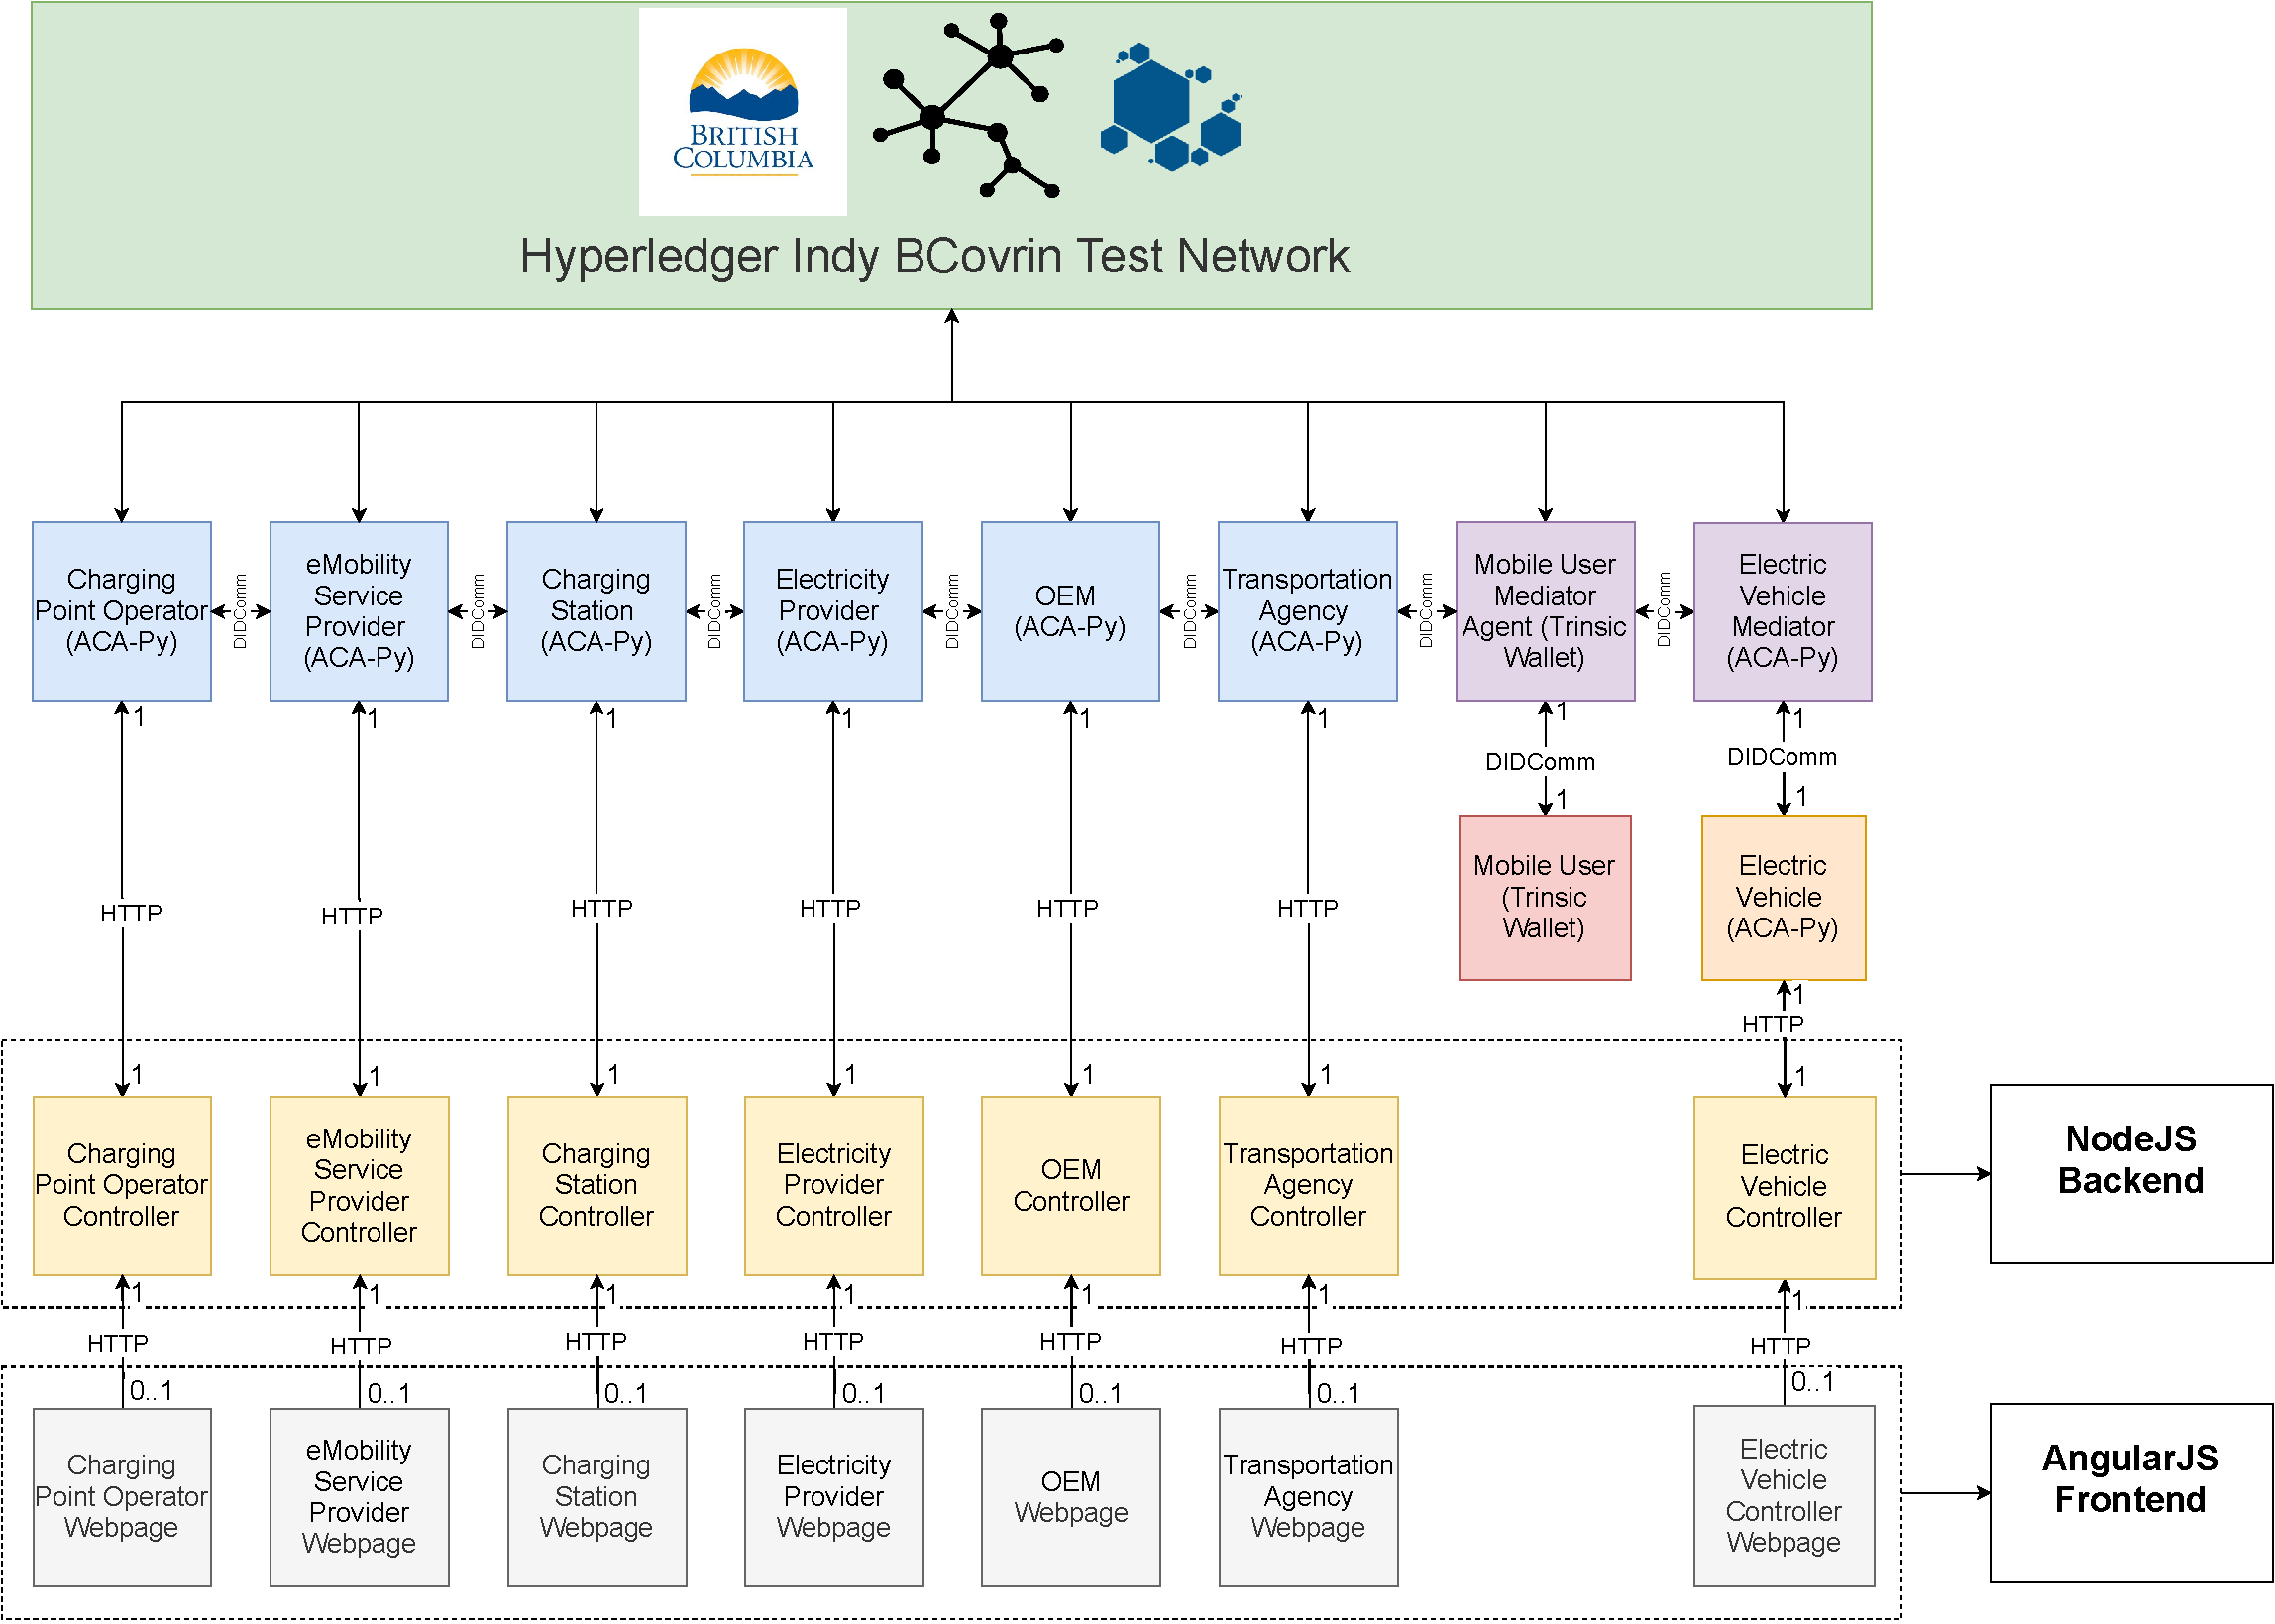
\includegraphics[keepaspectratio=true, width=\textwidth]{images/ImplementationArchitecture.pdf}
    \caption{Implementation Components Architecture and Protocols}
    \label{fig:Implementation_Architecture}
\end{figure}

\subsubsection{Agent Configuration}
\label{subsubsec:agent_configuration}

The parameters used to start-up the agents play a significant role in the necessary tasks needed to be performed by the controller (and in turn the developer). Within the content found on the ACA-Py repository, there are a great number of deployment parameters that can be set on startup. Here the configuration details of the agents are discussed and rationalized. For more information on each of the parameters it is recommended to look at the official startup parameters documentation\footnote{\url{https://github.com/hyperledger/aries-cloudagent-python/blob/main/DevReadMe.md\#about-aca-py-command-line-parameters}}. 

One of the most important things to mention in these parameters is the fact that for the sake of simplification and given that this implementation was created with the goal of being a proof-of-concept, multiple "auto-*" parameters have been set to true. This allows the agent to automatically perform certain actions, without the need of a controller. Although this helps demonstrate the functionalities of the agents, in a production level application it would be better to manually implement these actions.
% The following list of parameters was extracted from one example agent (the CPO agent), with the only parameters in need to change for the other agents being highlighted with an asterisk (*). 
In cases of mediation, if this connection is meant to be established on startup (which is the case with this proof-of-concept), then the \textit{open-mediation} and \textit{mediator-invitation} parameters needs to be set on the mediator and the mediated agents, respectively.

It is also relevant to mention that the agents have pre-configured webhook functionalities, that allow for a better interaction with the agents. After assigning a \textit{webhook-url} (which in theory should be assigned to the same endpoint as the controller that is running), it is possible to listen to specific webhook URLs and extract information about the different steps in the communications, and from that perform custom logic using the controller. One example of that is the basic messages exchanged between the CS and the CPO agents to obtain the charging rate fee (as depicted in Figure~\ref{fig:charging_and_billing_ssd} of Section~\ref{subsubsec:information-flows-ssi}).

\iffalse

\begin{itemize}
    \item General (for all agents)
    \begin{itemize}
        \item admin-insecure-mode: true
        \item admin: [0.0.0.0, 8018] *
        \item label: cpo.Agent *
        \item inbound-transport: - [http, 0.0.0.0, 8017] *
        \item outbound-transport: http
        \item endpoint: http://cpoagent10.ejemplo.me *
        \item genesis-url: http://test.bcovrin.vonx.io/genesis 
        \item seed: 0923456ERFDZSXCVTYUO9986OREDFCPO *
        \item auto-provision: true
        \item wallet-type: indy
        \item wallet-name: cpoWallet *
        \item wallet-key: 12345678 *
        \item tails-server-base-url: http://host.docker.internal:6543
        \item webhook-url: http://host.docker.internal:9229/cpo/webhooks *
        \item auto-accept-invites: true
        \item auto-accept-requests: true
        \item auto-ping-connection: true
        \item auto-respond-messages: true
        \item auto-respond-credential-proposal: true
        \item auto-respond-credential-offer: true
        \item auto-respond-credential-request: true
        \item auto-respond-presentation-proposal: true
        \item auto-respond-presentation-request: true
        \item auto-verify-presentation: true
        \item auto-store-credential: true
    \end{itemize}
    \item For Mediator Agents
    \begin{itemize}
        \item open-mediation: true
    \end{itemize}
    \item For Mediated Agents
    \begin{itemize}
        \item mediator-invitation: "http://evmediatoragent10.ejemplo.me?oob=eyJAd....fV19"
    \end{itemize}
\end{itemize}

\fi

\subsubsection{Adopted Aries RFCs}
\label{subsubsec:adopted_aries_rfcs}

All standards used in this solution follow the Aries RFCs Specifications (which have been marked as ACCEPTED at the time of writing) found in the appropriate GitHub repository\footnote{\url{https://github.com/hyperledger/aries-rfcs/blob/master/index.md}}. These RFCs are considered to be the standard for communication between Aries agents. The most relevant RFCs that explain how the agents can establish connections, send messages, issue credentials, verify credentials, be mediated, are highlighted below with a link to the appropriate RFC:

\begin{itemize}
    \item \textbf{Aries RFC 160: Connection Protocol} - In order for an agent to establish a connection with another, the communication flow follows the Aries RFC 160: Connection Protocol\footnote{\url{https://github.com/hyperledger/aries-rfcs/blob/master/features/0160-connection-protocol/README.md}}.
    \item \textbf{Aries RFC 095: Basic Message} - When an agent sends a message to another agent, it utilizes the Aries RFC 0095 - Basic Message\footnote{\url{https://github.com/hyperledger/aries-rfcs/blob/master/features/0095-basic-message/README.md}}.
    \item \textbf{Aries RFC 0036: Issue Credential Protocol 1.0} - The first iteration of the Issue Credential Protocol is used to explain the flow of messages needed to issue credentials from one agent to another. This protocol is still utilized in this proposed solution despite the introduction of version 2.0 of this RFC, since the Trinsic Wallet App only supports versions 1.0 of the protocols mentioned in this section\footnote{\url{https://github.com/hyperledger/aries-rfcs/blob/master/features/0036-issue-credential/README.md}}.
    \item \textbf{Aries RFC 0037: Present Proof Protocol 1.0} - This is the sibling RFC to the RFC 0036, since this utilizes the concepts explained in the latter to explain how a Holder can prove to a Verifier (remembering the roles explained in Section~\ref{subsubsec:verifiable_credential_model}) any claims\footnote{\url{https://github.com/hyperledger/aries-rfcs/blob/master/features/0037-present-proof/README.md}}.
    \item \textbf{Aries RFC 0453: Issue Credential Protocol 2.0} - The second iteration of the Issue Credential Protocol is used when an ACA-Py agent wishes to issue credentials to other ACA-Py agents. This version replaces the (indy-specific) filtration criteria with a generalized filter attachment to align with the rest of the messages in the protocol\footnote{\url{https://github.com/hyperledger/aries-rfcs/blob/master/features/0453-issue-credential-v2/README.md}}.
    \item \textbf{Aries RFC 0454: Present Proof Protocol 2.0} - As a second iteration of the Present Proof Protocol 1.0 protocol, this one is used between presentation requests between ACA-Py agents, since both support the usage of this protocol\footnote{\url{https://github.com/hyperledger/aries-rfcs/blob/master/features/0454-present-proof-v2/README.md}}.
    \item \textbf{Aries RFC 0046: Mediators and Relays} - In order to guarantee mediation between agents, used in the Electric Vehicle agent implementation, the communication flow between mediator and mediated agents is explained in detail in RFC 0046: Mediators and Relays\footnote{\url{https://github.com/hyperledger/aries-rfcs/blob/master/concepts/0046-mediators-and-relays/README.md}}.
    \item \textbf{Other Relevant RFCs} - Other RFCs are implicitly used when developing using the Aries framework, and are underlying to the agents communications. Therefore they have been abstracted from a detailed explanation but are worth revisiting in the official Aries RFCs repository as linked in the introduction to this section.
\end{itemize}

\subsubsection{Application Logic}
\label{subsubsec:application_logic}

Since the application relies on multiple parties, it is important to explain how the flow between the \textit{frontend - backend - agent} works, with the help of some use cases. The agents expose REST API endpoints which are used to trigger operations according to the agents documentation, as explained previously in Section~\ref{subsubsec:agent_configuration}. The controllers are all present in the same NodeJS project, which essentially has different endpoints, depending on the action that is meant to be performed, as in any REST API application. To provide a better understanding of how the application works, a small diagram in Figure~\ref{fig:flow_of_credential_issuance} contains the call stack between the different components in the use case of the Charging Station issuing a credential to the EVOwner at the end of the charging session.

\begin{figure}[!htb]
    \centering
    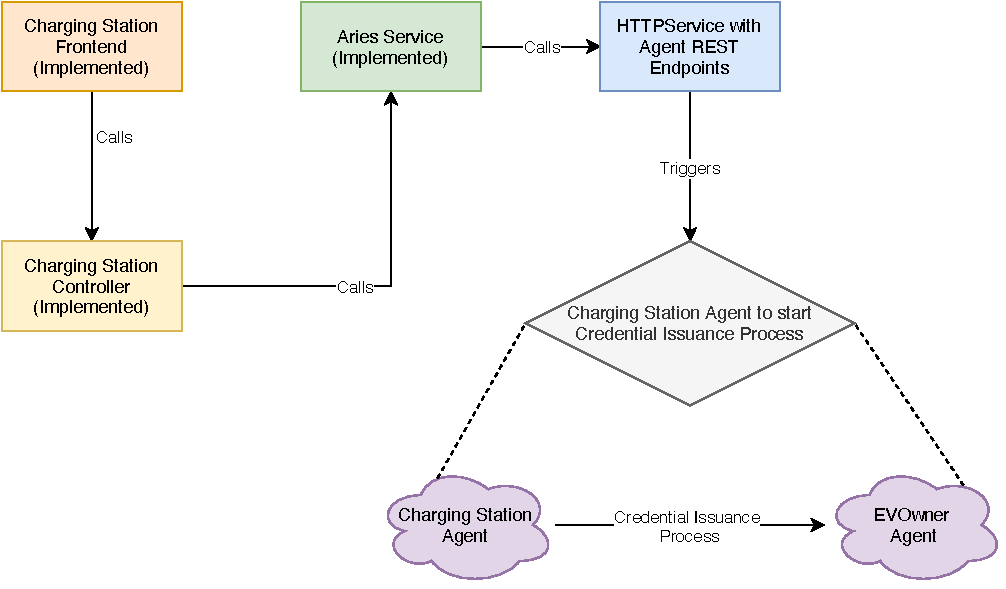
\includegraphics[keepaspectratio=true, width=0.8\textwidth]{images/FlowOfCredentialIssuance.pdf}
    \caption{Call stack to Start Credential Issuance Process}
    \label{fig:flow_of_credential_issuance}
\end{figure}

Starting off, the user triggers the action to issue the credential by pressing the button on the UI "Issue Receipt Credential". This will trigger the AngularJS function \textit{issueCredential} (as seen below) that will call the Angular Service to hit a NodeJS REST endpoint that is tailored for that event (function \textit{issueCredentialWithFields}). 

\begin{lstlisting}[language=JavaScript]
  issueCredential(): any {
    this.coreService.issueCredentialWithFields('cs', this.connectionId, 'receipt', this.eMSPContractID);
  }
\end{lstlisting}

\begin{lstlisting}[language=JavaScript]
  public issueCredentialWithFields(endpointName: string, connectionId: string, credentialEndpoint: string, contractID: string): any {
    try {
      return this.http.post(this.backendUrl + '/' + endpointName + '/issue-credential/' + credentialEndpoint, {"connectionId": connectionId, "eMSPContractID": contractID}, this.headers).toPromise();
    } catch (err) {
      console.log(err);
    }
  }
\end{lstlisting}

The code below is the controller code on the NodeJS backend that is listening to the endpoint hit previously by the frontend call (\textit{issue-credential/receipt}). Lines 4-10 represent the object that contains the attribute values for the receipt credential after a charging session. The object \textit{credentialOffer} in line 14 represents the object that is sent to the issuer agent, with information such as the connectionID (line 16) to the (to-be) holder of said credential. Other relevant information like the schemaID, credential definition ID and issuer DID (lines 21-23) are also present in this object. At last, the object is ready to be sent to the appropriate agent endpoint that handles the issuance of credentials. For this, the controller calls the implemented service (line 27) to perform the HTTP POST request that are used to interact with the agents.

\begin{lstlisting}[language=JavaScript]
    @Post('issue-credential/receipt')
    public issueCredentialReceipt(@Body("connectionId") connectionToEVOwner: any, @Body("eMSPContractID") eMSPContractID: any): Promise<CredentialExchange> {

        var credentialValues = [
            "0000000001",
            "00:30:00",
            this.currentChargingRate,
            "4€",
            eMSPContractID
        ]

        const credentialPreviewArray = this.credential7schema_attributes.map((key, i) => ({ name: key, value: credentialValues[i] }));

        const credentialOffer = new CredentialProposalRequestV1(false,
            "Charging Transaction Receipt",
            connectionToEVOwner,
            new CredentialPreview('issue-credential/1.0/credential-preview', credentialPreviewArray),
            {
                dif: { some_dif_criterion: '' },
                indy: {
                    schema_id: this.credential7schema_id,
                    cred_def_id: this.credential7credentialDefinitionID,
                    issuer_did: this.csDID
                }
            });

        return new Promise(resolve => {
            this.ariesService.sendCredentialV1(this.api, credentialOffer).pipe()
                .subscribe(responseSend => {
                    resolve(responseSend);
                }
                )
        }
        )
    }
\end{lstlisting}

After the service is called, the service is programmed to make use of the agents REST endpoints and have them perform the desired tasks, in the code below it is possible to see the generic implementation of how to have an agent start the issuance of credentials (with the V1 protocol version). After this point, the agent will handle the rest and the credential will be sent to the receiver agent.

\begin{lstlisting}[language=JavaScript]
        public sendCredentialV1(endpoint: string, credentialProposalRequest: CredentialProposalRequestV1): Observable<CredentialExchange> {
        return this.httpService
            .post(endpoint + "issue-credential/send", credentialProposalRequest)
            .pipe(map((response: AxiosResponse<CredentialExchange>): CredentialExchange => response.data))
            .pipe(
                catchError(e => {
                    throw new HttpException(e.response.data, e.response.status);
                }));
    }
\end{lstlisting}

\subsection{Deployment Details}
\label{subsec:deployment_details}

In this section the deployment details of the prototype will be highlighted, with instructions on how to replicate the behaviour of the system and what conditions to bear in mind when deploying the system from fresh. 

\subsubsection{Steps for the deployment}
\label{subsubsec:steps_for_the_deployment}

In order to deploy the system, a number of software/utilities are used. The system comprises of 6 components, which are containerized using Docker\footnote{\url{https://www.docker.com/}} and orchestrated using docker-compose\footnote{\url{https://docs.docker.com/compose/install/}}. These components are present in Figure~\ref{fig:docker-desktop} and contain the following:

\begin{itemize}
    \item postgres - a container that is running an instance of a postgres database, needed in case of backend persistent storage (if needed, to keep track of connection IDs, schema IDS and/or credential definition IDs).
    \item docker - this entry contains two instances that make for one tails-server\footnote{\url{https://github.com/bcgov/indy-tails-server}}, which is used as the revocation registry for the system, this is necessary otherwise revocation cannot be supported. This software stores and makes available tails files for use with Hyperledger Indy.
    \item aries-cloudagent-containers - this is an entry that comprises all eight agents that were created for this proof-of-concept, each agent is therefore a docker container.
    \item ssi-thesis-backend - a container that is running a NodeJS backend with the NestJS\footnote{\url{https://nestjs.com/}} framework, for the backend of the proof-of-concept.
    \item ssi-thesis-frontend - four containers that are running multiple instances of AngularJS\footnote{\url{https://angular.io/}} frontends, one for the main application, and three used to have a better interface of three of the agents states (connections, credentials, etc...).
\end{itemize}

\begin{figure}[!htb]
    \centering
    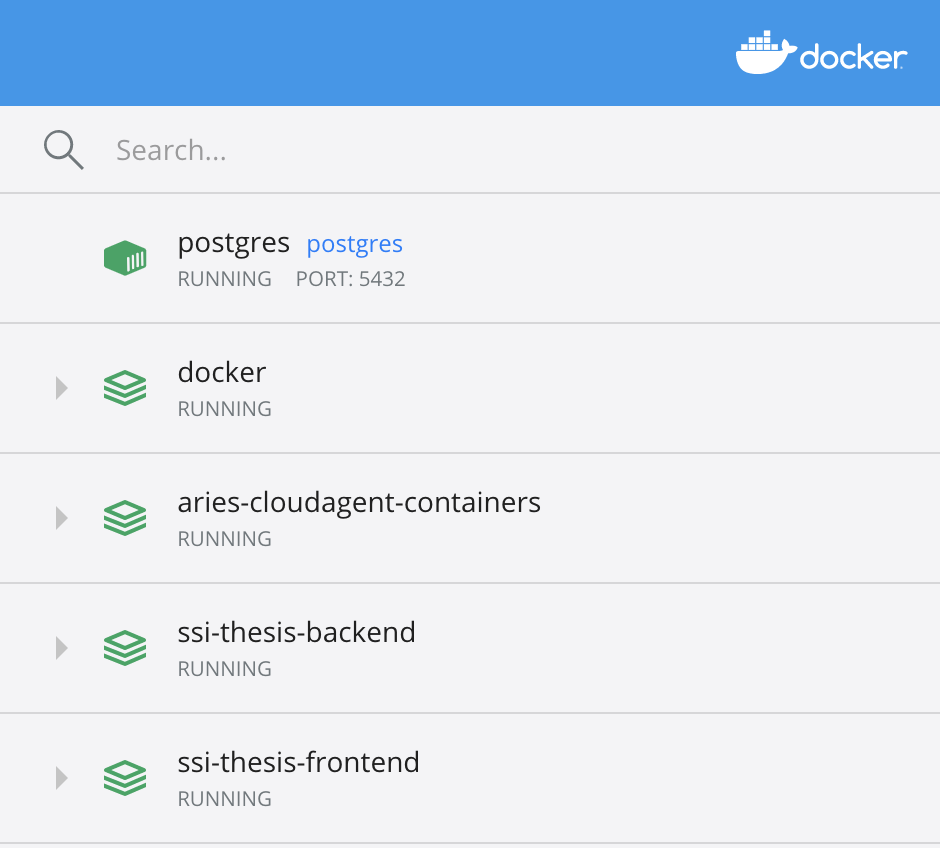
\includegraphics[keepaspectratio=true, width=0.5\linewidth]{images/docker-desktop.png}
    \caption{Docker Desktop with running containers}
    \label{fig:docker-desktop}
\end{figure}

In order to deploy these containers, the instructions are put together in different bash scripts\footnote{Used to curl specific endpoints to automate connections, issuance and verification of credentials for testing and demonstration purposes.} to automate the deployment of the application.

Given that the agents need to know how to interact with others using their own endpoints (or through the mediators endpoints), in a development environment these endpoints would be \textit{localhost:port}. But, to be able to access them from the outside, it was decided that using a tunneling software would make the solution more elegant and more close to reality. For this purpose, the open-source software pgrok\footnote{\url{https://github.com/jerson/pgrok}} was used. It offers free introspected tunnels to localhost, and this way the agents have their own fixed endpoint. 

For instructions on how to install the Trinsic Wallet Agent Mobile Application, please refer to the instructions on Appendix~\ref{app:trinsic_installation}, where a detailed description on how to setup the agent is provided.

The best source of code documentation is present in the GitHub repository that complements this manuscript. It contains all the necessary information on how to deploy the system and where changes need to be made depending on different scenarios.
Despite those instructions, a step-by-step guide will also be provided below.

\paragraph{Step 1: pgrok configuration}

To make sure the agents have their tunnels active before the start of the application, running the following line will start the tunneling service for each agent. This deployment follows the configuration created that will forward each agent's localhost port to a specific endpoint, exclusive for each agent. 

\begin{lstlisting}
pgrok -config=pgrok.yml start oemagent epagent evmediatoragent rdwagent csagent evagent emspagent cpoagent 
\end{lstlisting}

\begin{figure}[!htb]
    \centering
    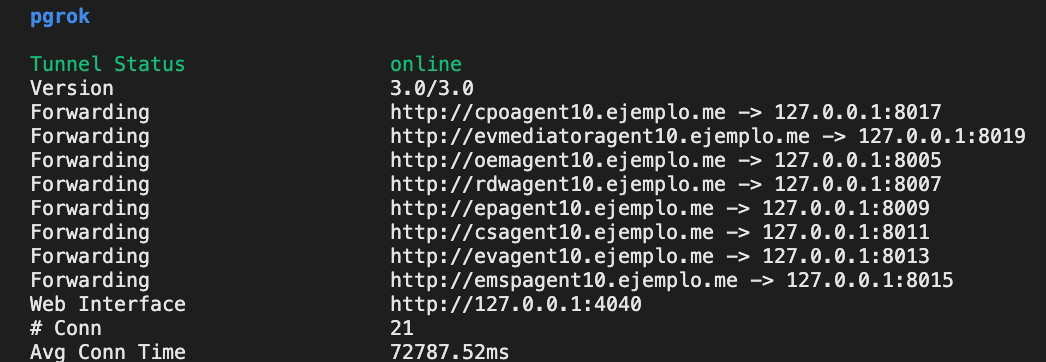
\includegraphics[width=0.6\linewidth]{images/pgrok.jpeg}
    \caption{pgrok in action, tunneling the localhost ports to specific endpoints, depending on the configuration}
    \label{fig:pgrok_image}
\end{figure}

\paragraph{Step 2: Configuration File}
This file is crucial for the systems operation. It is located in the backend implementation (\textit{ssi-thesis-backend/src/common/config/DefaultConfig.ts}). This is where the hard-coded information is written to, and from where the controller extracts information regarding:

\begin{itemize}
    \item Agents endpoints;
    \item Public DIDs;
    \item Credential Schema IDs and Credential Definition IDs;
    \item Connection IDs
\end{itemize}

\paragraph{Step 3: \textit{deployment.sh} script}

This script is in charge of deploying the revocation registry (tails-server), the agents, the backend, the postgres instance and the frontends.
Each agent is deployed according to a configuration file specific to each agent.
There is a particular step that is really important for the deployment of the agents. On startup, the mediator agent for the Electric Vehicle will create a mediation-invitation. This is printed in the command line and needs to be pasted to the \textit{mediator-invitation} field on the EVs agent deployment configuration file (\textit{ev.config.yml}). After pasting the mediatior-invitation to the configuration and pressing enter on the terminal, the deployment will carry on and both the EV and EV mediator agents mediation will be established.

\paragraph{Step 4: \textit{establish\_connections.sh} script}

For the sake of demonstrating the functionalities of the system, the agents connections are setup using a script, and the connection IDs are stored in a file for the agents to communicate between themselves. This script makes HTTP calls to the controller and that in turn makes contact with the agents to first create the connection invitations on the inviting agent, and receive the connection invitation on the receiver agent.
Each connection ID that is printed (as seen in Figure~\ref{fig:connections_screenshot}) needs to be pasted on the correct field on the Configuration File, as explained before.

\begin{figure}[!htb]
    \centering
    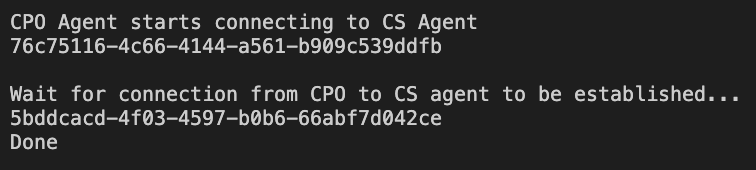
\includegraphics[width=0.6\linewidth]{images/connections_screenshot.png}
    \caption{How to extract the connection IDs after executing the script}
    \label{fig:connections_screenshot}
\end{figure}

\paragraph{Step 5: \textit{deploy\_schemas\_and\_credential\_definitions} script}

After setting the version number in the Configuration file (field "schema\_version"), the task of submitting schemas and credential definitions onto the ledger has been automated. The REST API calls the controller to create the schemas by making the calls to the agents' endpoints, this way the appropriate agent submits these onto the ledger (according to Table~\ref{tab:mapping_of_credentials} in Section~\ref{subsubsec:schemas_and_CDs}). Similar to the previous \textit{establish\_connections.sh} script, the shell script outputs the Schema IDs and the Credential Definition IDs that should be inserted into the Configuration file, as presented in Figure~\ref{fig:schemas_screenshot}.

\begin{figure}[!htb]
    \centering
    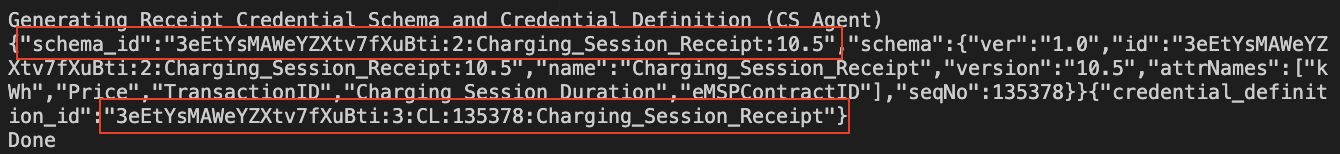
\includegraphics[width=0.8\linewidth]{images/schema_and_credential_definition.png}
    \caption{How to extract the schema and credential definition IDs after executing the script}
    \label{fig:schemas_screenshot}
\end{figure}


\subsubsection{Steps for running the use case scripts}
\label{subsubsec:steps_for_running_the_use_case_scripts}

After deploying the system, it is ready to power the use cases described in Section~\ref{subsubsec:information-flows-ssi}. The tasks that are conducted only between ACA-Py agents have been automated via shell scripts to hit the specific controller endpoints to trigger specific actions. All of the actions that require EV Owner interactions are meant to be used by means of the frontend instances deployed.

\paragraph{Step 1: \textit{service\_providers\_flow.sh} script}

This script triggers the "Service Providers Flow" explained in Section~\ref{paragraph:service_providers_flows_with_ssi}, only from the eMSP, CPO, EP and CS perspectives.

It starts with the eMSP issuing the Contract with CPO credential to the CPO.

\begin{lstlisting}[language=bash]
#Issue Contract with CPO to CPO from EMSP (CREDENTIAL 5)
curl -s -XPOST -H "Content-type: application/json" 'localhost:9229/emsp/issue-credential/cpo' > /tmp/output.html

printf '\nCredential is being issued from EMSP to CPO...\n'
sleep 2
printf '\nDone\n'
\end{lstlisting}

Then the CPO issues a credential to the Charging Station to attest its ownership.

\begin{lstlisting}[language=bash]
#Issue Ownership of CS to CS from CPO (CREDENTIAL 6)
curl -s -XPOST -H "Content-type: application/json" 'localhost:9229/cpo/issue-credential/ownership-cs' > /tmp/output.html

printf '\nCredential is being issued from CPO to CS...\n'
sleep 2
printf '\nDone\n'
\end{lstlisting}

And at last, the EP issues a Contracting Credential to the CPO.

\begin{lstlisting}[language=bash]
#Issue Contract with CPO to CPO from EP (CREDENTIAL 8)
curl -s -XPOST -H "Content-type: application/json" 'localhost:9229/ep/issue-credential/contract-cpo' > /tmp/output.html

printf '\nCredential is being issued from EP to CPO...\n'
sleep 2
printf '\nDone\n'
\end{lstlisting}

To complete the rest of the use case, the EV Owner performs the steps listed below. Note that visual representations of each step can be found in Appendix~\ref{subapp:service_providers_flow}:

\begin{enumerate}
    \item Navigate to the frontend's URL (localhost:4200)
    \item Select the eMSP portal (Figure~\ref{fig:service_provider_screenshot_1}).
    \item Connect to the TA Agent using the QR Code, scanning it with the Trinsic Wallet App (Figure~\ref{fig:service_provider_screenshot_2}).
    \item Press the "Issue Credential" button (Figure~\ref{fig:service_provider_screenshot_3}) and accept the credential on the Trinsic Wallet App (Figure~\ref{fig:service_provider_screenshot_4}).
\end{enumerate}

\paragraph{Step 2: \textit{ev\_interactions.sh} script}

This script triggers the "EV Owner and EV Interactions with SSI" explained in Section~\ref{paragraph:ev_owner_and_ev_interactions_with_ssi}, only from the EV, OEM and TA perspective.

It starts with the OEM agent issuing the VIN Credential to the Electric Vehicle.

\begin{lstlisting}[language=bash]
#Issue VIN Credential to EV from OEM (CREDENTIAL 1)
curl -s -XPOST -H "Content-type: application/json" 'localhost:9229/oem/issue-credential/send' > /tmp/output.html
printf '\nCredential is being issued from OEM to EV...\n'
sleep 2
printf '\nDone\n'
\end{lstlisting}

Then, the TA verifies this credential, and issues another credential to attest the EVs registration.

\begin{lstlisting}[language=bash]
#RDW Verify VIN Credential and Issue EV Registration to EV from RDW (CREDENTIAL 2)
printf '\nRDW is requesting VIN credential from EV\n'
curl -s -XPOST -H "Content-type: application/json" 'localhost:9229/rdw/present-proof/send-request'  > /tmp/output.html
printf '\nRequest sent, waiting for reply from EV\n'
\end{lstlisting}

To complete the rest of the use case, the EV Owner performs the steps listed below. Note that visual representations of each step can be found in Appendix~\ref{subapp:ev_owner_and_ev_interactions}:

\begin{enumerate}
    \item Navigate to the frontend's URL (localhost:4200)
    \item Select the TA portal (Figure~\ref{fig:ev_owner_screenshot_1}).
    \item Connect to the TA Agent using the QR Code, scanning it with the Trinsic Wallet App (Figure~\ref{fig:ev_owner_screenshot_2}).
    \item Press the "Issue Credential" button (Figure~\ref{fig:ev_owner_screenshot_3}) and accept the credential on the Trinsic Wallet App (Figure~\ref{fig:ev_owner_screenshot_4}).
\end{enumerate}

\paragraph{Step 3: Performing the "Charging and Billing" flow}

This part of the system does not rely on any scripts, but rather just the EV Owner interacting with the frontend and the Trinsic Wallet App.

The steps are already described in Section~\ref{paragraph:charging_and_billing_flow_with_ssi}, but a link between the steps and the screenshots of the frontend and the Trinsic Wallet App will be made below, similarly to what was done for the previous two scripts above.

To complete this use case, the EV Owner performs the steps listed below. Note that visual representations of each step can be found in Appendix~\ref{subapp:charging_and_billing}:

\begin{enumerate}
    \item Navigate to the frontend's URL (localhost:4200)
    \item Select the Charging Station Dashboard (Figure~\ref{fig:charging_screenshot_1.0}).
    \item Connect to the Charging Station Agent using the QR Code, scanning it with the Trinsic Wallet App (Figure~\ref{fig:charging_screenshot_1.1}).
    \item Press the "Request Proofs" button (Figure~\ref{fig:charging_screenshot_2}).
    \item Receive the two presentation requests (Figure~\ref{fig:charging_screenshot_3}), and accept the Request for the Contract with eMSP credential (Figure~\ref{fig:charging_screenshot_3.1}) and the EV Owner Registration at the TA one (Figure~\ref{fig:charging_screenshot_3.2}).
    \item At the Charging Station Dashboard, press the "Verify Proofs" button (Figure~\ref{fig:charging_screenshot_4}).
    \item The credentials have now been verified by the agent as seen on the screen, as well as the eMSP Company name is presented on the screen (Figure~\ref{fig:charging_screenshot_5}).
    \item Now that the Company Name is known, the EV Owner may request the current charge rate pressing the "Obtain Current Charge Rate" button (Figure~\ref{fig:charging_screenshot_6}).
    \item The price/kWh is presented on the screen (Figure~\ref{fig:charging_screenshot_7}).
    \item The EV Owner presses "Request EV Credentials" (Figure~\ref{fig:charging_screenshot_8}) so that the Charging Station can request from the EV agent a presentation to attest it is the same vehicle as indicated by the EV Owner.
    \item After a few seconds, the EV Owner presses "Verify Proofs" to verify if the process has been concluded.
    \item The credential from the EV has now been verified by the CS agent as seen on the screen, as well as the registration number is presented on the screen together with the EV Owner registration number (Figure~\ref{fig:charging_screenshot_9}).
    \item Now the EV Owner may start charging the EV, pressing the "Start Charging" button (Figure~\ref{fig:charging_screenshot_10}).
    \item The Charging Station will start the charging and stop it right away (Figure~\ref{fig:charging_screenshot_11}).
    \item The EV Owner can now issue a receipt credential, pressing the "Issue Receipt Credential" button (Figure~\ref{fig:charging_screenshot_12}).
    \item On the Trinsic Wallet App, the EV Owner will receive a credential offer (Figure~\ref{fig:charging_screenshot_13}).
    \item The EV Owner accepts the credential by clicking the "Accept" button (Figure~\ref{fig:charging_screenshot_14.0}) and the credential is stored on the Trinsic Wallet App (Figure~\ref{fig:charging_screenshot_14.1}).
    \item An overview of the final state of the Charging Station dashboard in the good-case scenario can be found in Figure~\ref{fig:charging_screenshot_15}.
\end{enumerate}





\section{Evaluation}
\label{section:evaluation}

In this chapter the system designed in Chapter~\ref{section:design_and_implementation} and implemented in Chapter~\ref{sec:implementation_and_deployment_details} will be evaluated. First the methodology of this evaluation will be documented and then the results are demonstrated.

The evaluation will refer to a particular use case presented in Section~\ref{subsec:implementation_details}. The evaluation for the general SSI with IoT architecture presented in Section~\ref{subsec:architecture_for_ssi_with_iot} will be discussed at the end of this chapter. 

\subsection{Methodology}
\label{subsec:methodology}

% In order to evaluate a system that relies heavily on open-source software and whether the requirements are satisfied with the assumptions that were made, the evaluation does not regard benchmarking the actual proof-of-concept system, but rather assessing if the main components used can comply with the requirements listed in Chapter~\ref{sec:requirement_elicitation}.

The evaluation will be split into three distinct steps:

\begin{itemize}
    \item Benchmark the "Hyperledger Indy Network" and "Hyperledger Aries Cloud Agent - Python" in order to assess performance-, scalability- and availability-related NFRs;
    \item Qualitative evaluation of the proposed solution from domain experts;
    \item Cross-check requirements against the decisions taken throughout the project (and evaluation results).
\end{itemize}

\paragraph{Benchmark "Hyperledger Indy Network" and "Hyperledger Aries Cloud Agent - Python"}

This part of the evaluation will be made possible with the help of the development team of Hyperledger Indy, since performance and scalability tests were already made to the network. The results from these tests will be presented to validate the Non-Functional Requirements of the system.

Given that the agents are a core part of the system, being able to know the time they take to perform their tasks is imperative to know if these can be used at scale.

\paragraph{Qualitative evaluation from domain experts}

In order to measure the validity of the new system, and whether it can actually be considered an improvement to the current implementation (dissected in Section~\ref{subsec:case_description}), a qualitative assessment from domain experts is a vital part of understanding whether some assumptions are valid, feasible or impossible. 
This evaluation process consisted of:
\begin{itemize}
    \item Gathering contacts from various domain-specific experts that are related to the targeted use case (Energy, Blockchain, Self-Sovereign Identity).
    \item Inviting contacts to participate in the evaluation process, by having them sign up via a Google Forms with preliminary assessment questions, to profile the participants.
    \item Recording a presentation of the project with a small demo to send to the interested participants.
    \item Sending the interested evaluators the recorded presentation and demo, together with a Google Forms to assess their perspective on certain aspects of the system. 
\end{itemize}

\paragraph{Cross-check requirements} 

For this part of the evaluation, each requirement will be analyzed and discussed, to understand whether in the novel architecture of the system that given requirement is (partially) met, or not.


\subsection{Benchmark "Hyperledger Indy Network" and "Hyperledger Aries Cloud Agent - Python"}
\label{subsec:benchmark_hyperledger_indy_and_aries}

\paragraph{Hyperledger Indy Network evaluation}

As mentioned before, assessing the capability of the network that is the backbone of the proposed solution is a major part of understanding if it can handle the proposed use case requirements. Investigating performance tests made to the network landed on an issue on the Indy's JIRA repository. 
Issue \textbf{INDY-1343 - Prove production stability of an Indy network}\footnote{\url{https://jira.hyperledger.org/browse/INDY-1343}} arose from the following need: \textit{"Before encouraging people to use the Sovrin network for live loads, we need to prove that it will be stable under conditions similar to production use."} 
Sovrin's name has been highlighted previously in the Related Work chapter (Section~\ref{subsubsec:hyperledger_indy_sovrin}), and corresponds to the production level network created by the Sovrin Foundation.

The tests had mixed conclusions, with certain scenarios underperforming while others achieving the expected TPS throughput. After these tests, three more issues were lifted on the project's JIRA repository related to testing the performance of the network, INDY-1388\footnote{\url{https://jira.hyperledger.org/browse/INDY-1388}}, INDY-1607\footnote{\url{https://jira.hyperledger.org/browse/INDY-1607}} and INDY-2214\footnote{\url{https://jira.hyperledger.org/browse/INDY-2214}}. Table~\ref{tab:benchmarks_indy} contains information on the issues regarding network stability and their current status. It is worth noting that the latest issue (INDY-2214) has yet to be resolved, since December 2019. A detailed description of the tests can be found in a Google Sheets shared by the development team, that highlights their findings\footnote{\url{https://docs.google.com/spreadsheets/d/1DTjDsLSysFBiKU-9z4-IzunJk4wEy44hE_PGZYxnN_8/edit\#gid=1813415708}} (Available on 13th June 2021).

\begin{table}[t]
    \centering
    \begin{tabular}{|ccc|}
    \hline
        Issue \# & Title & Status \\
        \hline
        INDY-1343 & Prove production stability of an Indy network & \greencheck \\
        INDY-1388 & Prove stability under a DOS of an Indy network & \greencheck \\
        INDY-1607 & Proof of stability under load & \greencheck \\ 
        INDY-2214 & Repeat: Prove production stability of an Indy network & - \\
        \hline
    \end{tabular}
    \caption{Issues on Indy's JIRA Repository related to benchmarking the network}
    \label{tab:benchmarks_indy}
\end{table}

Although arguably the JIRA or the project's GitHub repositories are usually the best source of information regarding benchmarking tests, the best source to validate the current state of the Hyperledger Indy network comes directly from the Sovrin's foundation network status dashboard\footnote{\url{https://sovrin.org/ssi-metrics-dashboards/}}. Figure~\ref{fig:sovrin_metrics} demonstrates the network status from 12th June 2020 to 12th June 2021, regarding various metrics. The most relevant information regards the read and write availability, that achieves an outstanding \textbf{99.999\% read and write availability}.

\begin{figure}[!htb]
    \centering
    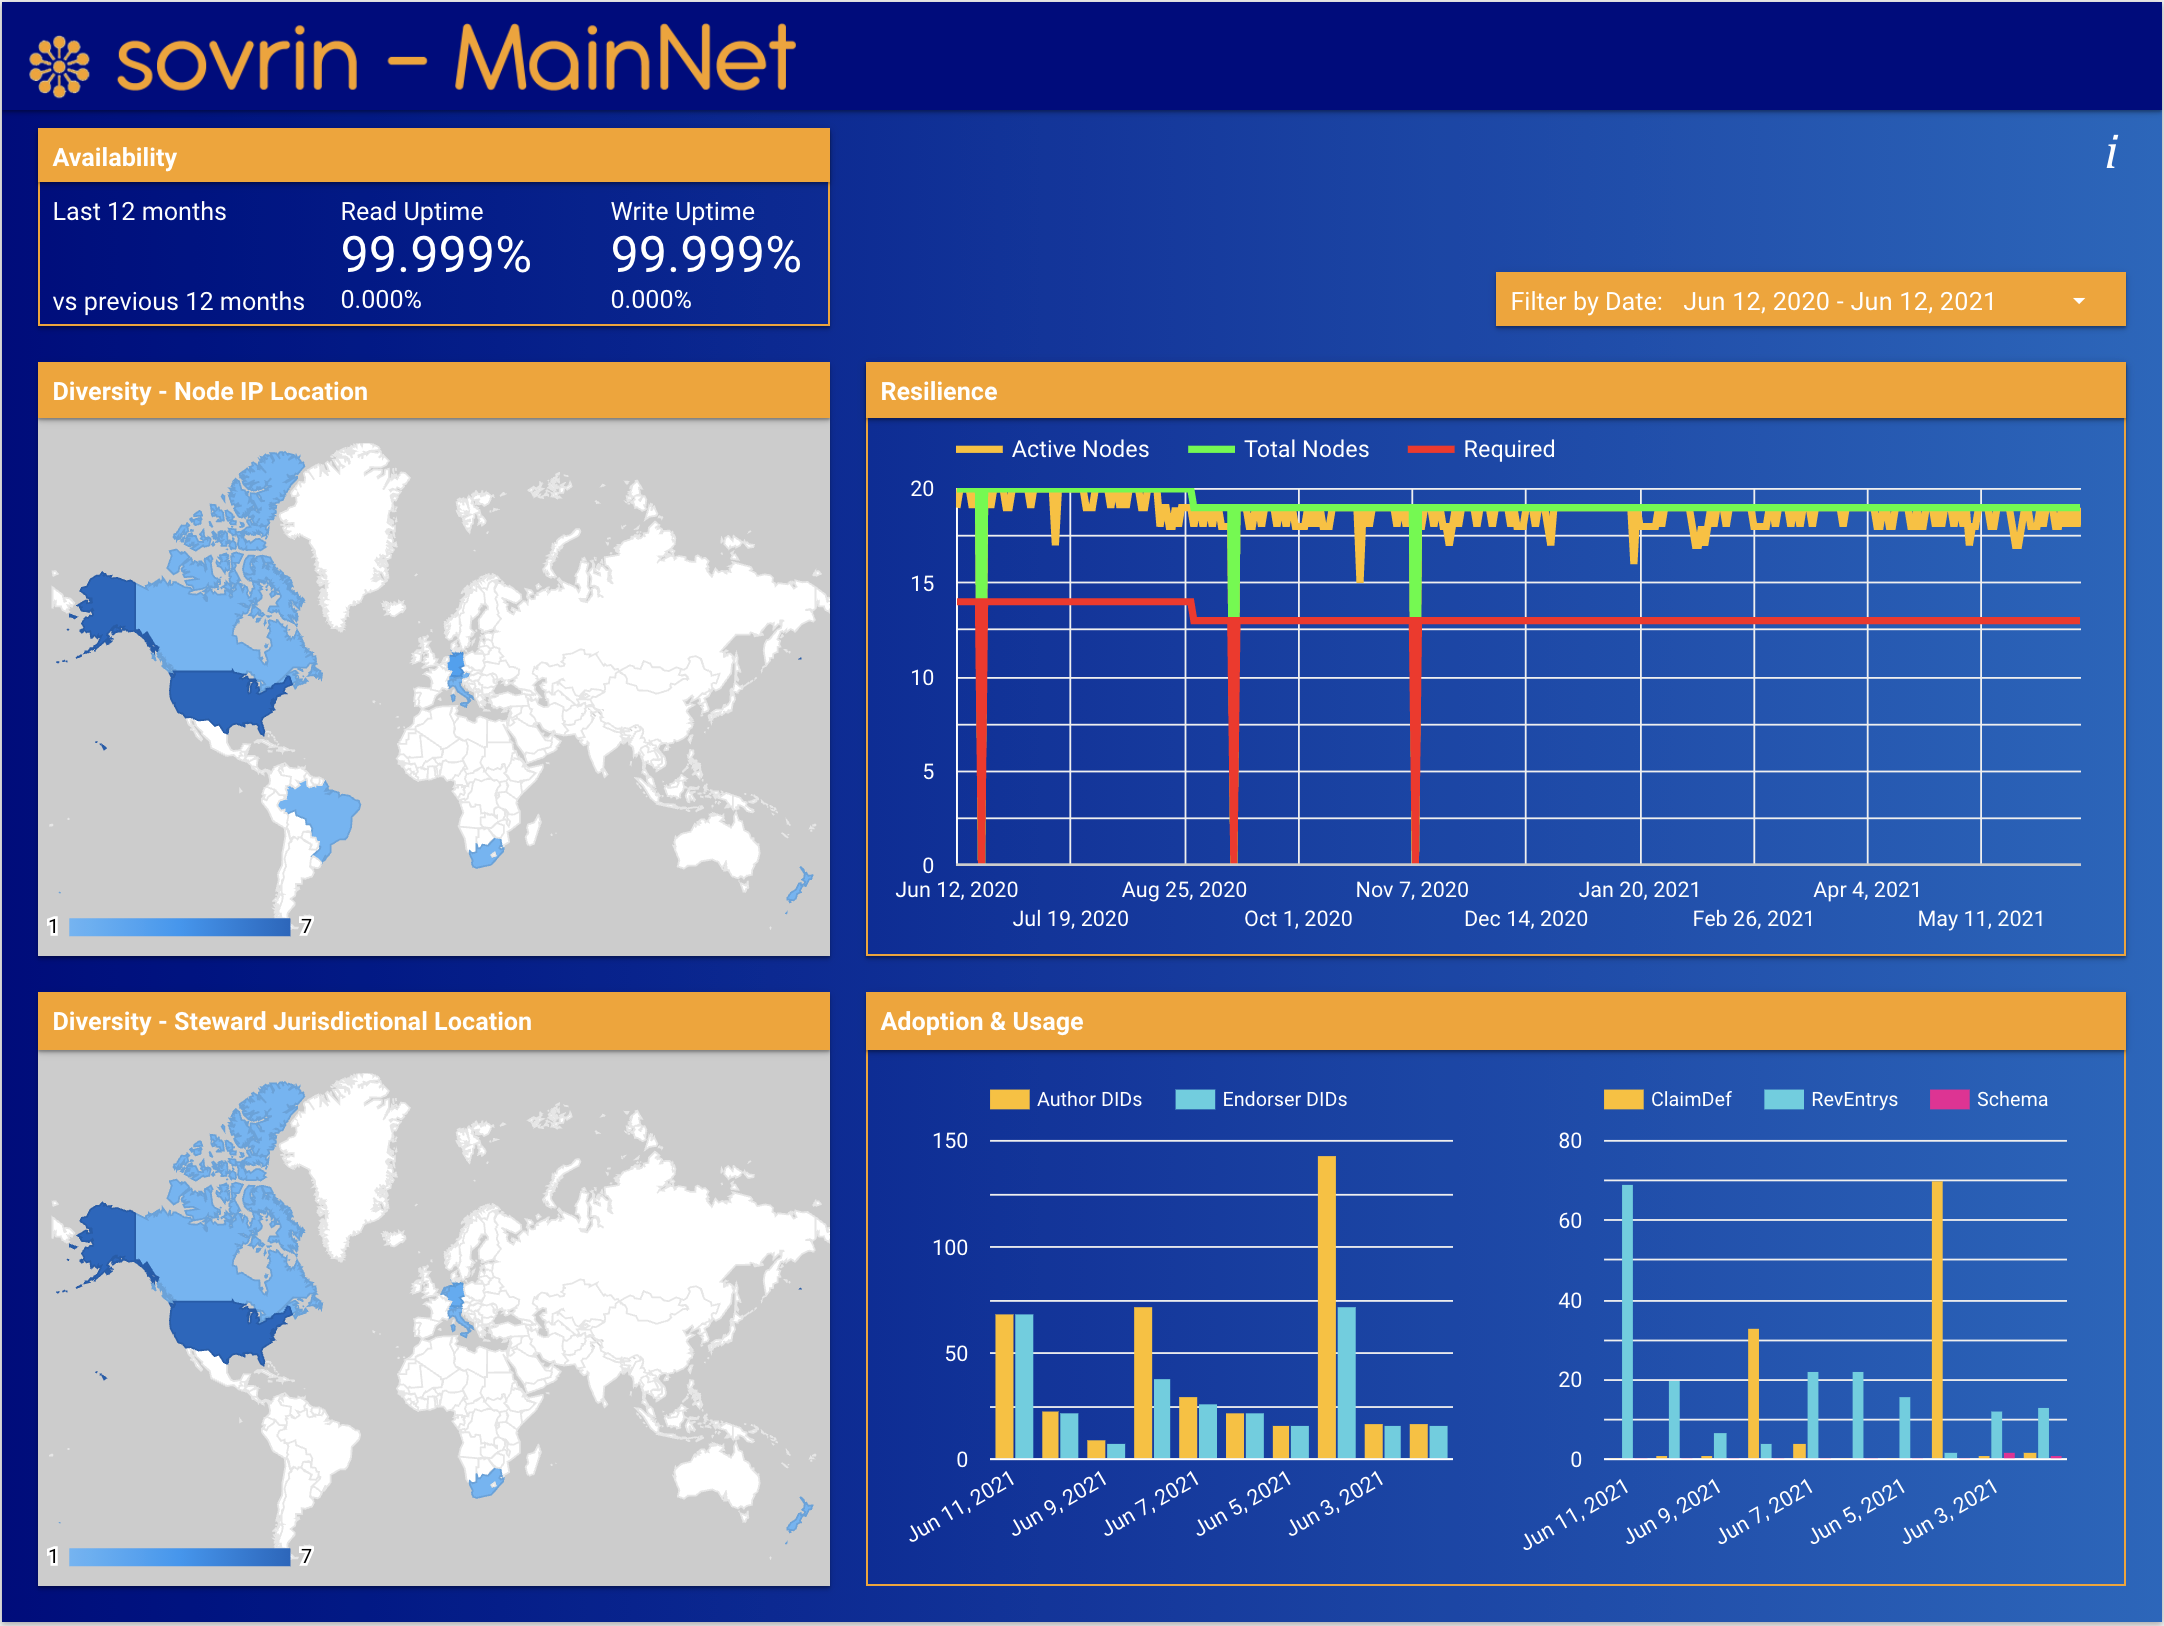
\includegraphics[width=0.8\linewidth]{images/sovrin_metrics.png}
    \caption{Sovrin Network (Hyperledger Indy nodes) metrics from 12 June 2020 to 12 June 2021}
    \label{fig:sovrin_metrics}
\end{figure}

\paragraph{Hyperledger Aries Cloud Agent - Python evaluation}

In order to assess the performance of the agent implementation, two different methods were used: Use the performance benchmark tests provided by the development team; and measure the times when conducting actions with the agents in the proof-of-concept implementation.

For the first, in the original Aries Cloud Agent - Python repository the developers included a basic \textit{performance.py} script that deploys two agents, and has one issue a predefined number of credentials to the other. These benchmarks are therefore a good indication of the times taken to issue credentials from one agent to another, and can vary depending on whether there is mediation between the two agents or not, and also if the credentials are revoked after they are issued.
This latter also indicates the feasibility to revoke credentials, something that was not explored in-depth with the proof-of-concept. 
For the second set of benchmarks to the agent implementation, the interactions of the agents will be timed manually to assess the performance requirements. The commands used to execute each of the runs, as well as more details extracted from the runs are listed in Appendix~\ref{app:benchmark_runs}.
In this appendix the computer specifications are also listed for reference. 

Looking at the results found in Table~\ref{tab:overview_of_different_attempts}, it is possible to see that an ACA-Py agent is able to issue credentials to another agent in an acceptable time, averaging 0.23s in three of the runs and 0.26s in the last. Note that these results are limited by the fact that the agents are running in the same piece of hardware, which may lead to an improvement in the times. Still, the results are 10 times faster than the time of interactions of the current system's validation periods, as listed in \textbf{Requirement NFR-2.4} - \textit{The process of validation the client's credentials should not take longer than the original method (designed for 2 seconds, with the worst case scenario being 30 seconds)}. For this reason, it is possible that the times may increase in a production environment, but not exceeding the optimal range of values.

\begin{table}[t]
    \centering
    \begin{tabular}{|ccccc|}
    \hline
        Run \# & Revocation & Mediation & Count & Average Credential Times \\
        \hline
        1 & \redcheckk & \greencheck & 1000 & 0.23s \\
        2 & \greencheck & \redcheckk & 1000 & 0.23s \\
        3 & \redcheckk & \redcheckk & 1000 & 0.23s \\
        4 & \greencheck & \greencheck & 1000 & 0.26s \\
        \hline
    \end{tabular}
    \caption{Overview of the different attempts}
    \label{tab:overview_of_different_attempts}
\end{table}

Besides these tests made to the credential issuance process, the actions needed for the charging process were also manually timed. 
When performing the charging process, the "Request Proofs" action from the EV Owner took on average less than 2 seconds. Note that this step occurs between an ACA-Py agent and a Trinsic Wallet agent.
For the process of the "Request EV Credentials" from the EV agent, this process also takes less than 2 seconds on average. This process involves the CS agent sending the request for the proof, the EV agent generating the proof, sending it back to the CS agent and then it being verified. 
At last, the "Issue Receipt Credential" process from the CS to the EV Owner's Trinsic Wallet agent also takes on average less than 2 seconds, but depends on the internet signal at the time of receiving the credential proposal on the Trinsic Wallet App dashboard.

\subsection{Qualitative Evaluation from domain experts}
\label{subsec:qualitative_evaluatin_from_domain_experts}

In this section the results from the evaluation provided by the domain experts will be presented to extract results that can validate the requirements.

\subsubsection{Preliminary Form Results}
\label{subsubsec:preliminary_form}

In the preliminary form shared with potential participants to the evaluation, the questions mostly related to profile questions, to understand the area expertise of the evaluators and how well they are aware of the charging process of EVs.
A total of six (6) people responded to the form, confirming their willingness to evaluate the proposed solution. Note that some of the participants had expertise in more than one area as demonstrated by Table~\ref{tab:expertise_of_evaluators}.

\begin{table}[!htb]
    \centering
    \begin{tabular}{|cc|}
    \hline
    Field of Expertise & Count \\
    \hline
    Blockchain & 4 \\
    Energy & 3 \\
    Self-Sovereign Identity & 1 \\
    Architecture & 1 \\
    EV Automotive & 1 \\
    \hline
    \end{tabular}
    \caption{Expertise of the Evaluators}
    \label{tab:expertise_of_evaluators}
\end{table}

From the six respondents, the follow data was extracted:

\begin{itemize}
    \item 3 out of 6 responded to be able to "teach someone else" about blockchain.
    \item 2 out of 6 responded to be able to "teach someone else" about Self-Sovereign Identity.
    \item None of the respondents own an EV, but more than half (4) of them are knowledged in the process of charging an EV. Out of those 4 people, 4 are aware of (most of) the parties in the process, 3 know how to charge an EV, and only 2 of them are aware of the current payment model.
\end{itemize}

\subsubsection{Results from experts' evaluation of system}
\label{subsubsec:results_from_experts_evaluation_of_system}

After gathering the profiles of the six evaluators, a video containing a pre-recorded slide presentation explaining the project was shared with the latters. In this video it was included part of the proof-of-concept's demonstration of how an EV Owner is able to charge its EV making use of Verifiable Credentials to attest the claims explained in the flow present in Section~\ref{paragraph:charging_and_billing_flow_with_ssi}.

This expert evaluation was mostly used to assess the usability requirements as well as the business value of the novel architecture. From the six (6) evaluators that agreed to answer the preliminary form, the following results arose:

When asked to prioritize "Ease of Use", "Data Privacy", "Cost Transparency", "Availability" and "Integration with Mobile Applications" in  an EV Charging Network from the least important (1) to the most important (5), these were the results:

\begin{itemize}
    \item Availability and Cost Transparency both obtained 23 points, making these two the most prioritized quality attributes;
    \item Ease of Use obtained 22 points, close to the first two quality attributes.
    \item Data Privacy and Integration with Mobile Applications scored 14 and 8 points, respectively, demonstrating that these two are not the highest priority for the evaluators.
\end{itemize}

The questions below constitute the questionnaire made to the evaluators. Each of them was given an ID.

\begin{itemize}
    \item \#1 - \textit{How understandable is the presented solution, from a user and business perspective?}
    \item \#2 - \textit{How do you think the solution compares with the current implementation of the network?}
    \item \#3 - \textit{With this solution, would you feel confident your personal data is protected?}
    \item \#4 - \textit{With this solution, would you consider the process of charging the vehicle more transparent?}
    \item \#5 - \textit{Do you consider the employed payment model user-friendly?}
    \item \#6 - \textit{Which feature(s) from this solution did you appreciate the most?}
    \item \#7 - \textit{Which feature(s) would you like to see added to this solution?}
    \item \#8 - \textit{Do you have any other comments on the presented solution?}
\end{itemize}


From the aforementioned questions, the more relevant finding were:

\begin{itemize}
    \item 4 out of 6 believe that the solution is "Very easy to understand" from a user perspective while 3 out of 6 thought the same from a business perspective.
    \item 4 out of 6 believe that the new solution is much better than the current implementation of the network.
    \item At least 6 out of 6 "Agree" with question \#3, with 3 of them selecting "Strongly Agree".
    \item The same results from question \#3 were obtained for question \#4.
    \item 5 out of 6 "Agree" to question \#5 regarding the user-friendliness of the payment model.
    \item The feature with the most appreciation was the "Added more transparency with the addition of the kWh price" feature, with 4 evaluators selecting that option for question \#6. 3 evaluators also enjoyed the "Removal of Login", 2 selected "Added Vehicle and Owner verification for extra security" and 1 liked the "Removal of external party - Maximising revenue" feature. None of the evaluators saw great value in the "Added receipt-credential to the end of the transaction".
\end{itemize}

For question \#7 regarding possible future features to add, the comments made by the evaluators are found below.

\begin{spverbatim}
"I know that right now there is a solution to have multiple suppliers per charge poll and users can charge their cars in different location. So an approach is based on you credentials and your supplier contract, this should be easy to identify and get a message saying you are now charging your car with supplier A in this rate."
    
"Using a unique vehicle identity in the process might give away the owner or driver, compromising privacy. Zero-knowledge might help alleviate that iff the vehicle ID is not anyway shared with the charging station."

"Include price options in case you are not in a hurry to charge and the network can use the optimal moment to charge, although that is not really related to the SSI part."

"try to remove as much steps in the user interaction as possible."

\end{spverbatim}

For question \#8 regarding additional comments or the overall appraisal of the system, the comments made by the evaluators are found below.

\begin{spverbatim}
"The overall process is well thought-out and nicely implemented."

"I understand the value of SSI for identifying myself as the owner or the car and the one charging it, however what is the benefit of sharing the receipt as a VC? That is also shared with the energy supplier, right? Or is that to resolve a dispute on the invoice in case the supplier charges you more? Or do you see scenario's where I would need to share that with some other party?"

"Excelent demo showing the way forward for EV charging"

"Although data privacy is not a major requirement for me, I would still prefer to have something that protects me as per your solution than what is currently in the market today"

"Need to think about multiple users of a single vehicle and also Fleet driver use case."

\end{spverbatim}

The overall assessment of this evaluation method allowed to understand how domain experts in the area perceive the system, which in turn granted good prospects to fulfill the necessary requirements. All evaluators provided valuable feedback and the consensus was that the solution is an improvement to the previous iteration, providing more transparency to the system and improved the user's experience with the system. The privacy limitations regarded in the comments will be addressed at a later stage, when cross-checking the requirements.


\subsection{Cross-check requirements}
\label{subsec:cross-check-requirements}

In this section, the requirements listed in Section~\ref{subsec:list_of_requirements_and_decisions} will be evaluated, and a link to the respective motivation and rationales is traced to a more detailed description that will be found in Appendix~\ref{app:requirement_evaluation}. These motivations reflect whether the specific requirement is satisfied or not using the decisions taken across the document (from technological, architectural or assumptions). For more information regarding the assessment of each requirement, the appendix contains all the necessary information for that purpose. Despite that, a few of the most important requirements will be discussed to highlight the most important decisions.

For both upcoming sections, a table has been made containing a mapping between the RequirementID, the priority of the requirement, the approval status and a link to the respective detailed table on the appendix. 
Below it is possible to find a legend for the different status symbols and their meaning.

\begin{itemize}
    \item \greencheck : Requirement fulfilled
    \item \textbf{-} : Needs further investigation or inconclusive
    \item \redcheckk : Requirement not fulfilled
\end{itemize}

\subsubsection{Functional Requirements}
\label{subsubsec:evaluation_functional_requirements}

Table~\ref{tab:full_requirements_evaluation_table(FR)} contains the aforementioned table, and it is possible to observe that regarding the Functional Requirements, almost all of the requirements were met, with the exception of one whose priority is a "Could have" and another which is prioritized as a "Must have".

Starting with the most important requirements that were fulfilled, the ones that add more value to the novel system and eliminate the liabilities presented in the case description in Section~\ref{subsubsec:current_liabities} are \ref{evaluation:FR-1.2}, \ref{evaluation:FR-1.4}, \ref{evaluation:FR-3.1} and \ref{evaluation:FR-5.1}. Requirement~\ref{evaluation:FR-1.2} reflects on the fact that now the EV Owner is presented with a kWh rate before the charging session takes place, allowing the owner to decide whether to charge the EV at that time. This price is dependant on the contracted eMSP company, given that different companies might obtain better contracts with the CPOs and provide better prices for their clients. Requirement~\ref{evaluation:FR-1.4}'s fulfillment provides a way for the EV Owners to obtain a receipt at the end of each charging session, in the form of a Verifiable Credential. This allows the client to obtain proof of that transaction, with information regarding the full price of the charging session, providing more transparency to the latter. Requirement~\ref{evaluation:FR-3.1} addresses the fact that the EV Owner now is forced to prove ownership of the EV in order to charge the vehicle, giving the system an extra layer of security, preventing thieves from charging stolen EVs. Requirement~\ref{evaluation:FR-5.1} concerns matters of privacy, since Personally Identifiable Information (PII) should not be written to any publicly accessible repository, to comply with current privacy regulations. This matter is fulfilled with the current SSI implementation, that only writes credentials and private DIDs (PII) to the entity's wallet and not in the DLT itself, complying with this requirement. For the requirements that were not addressed by the system (\ref{evaluation:FR-3.3} and \ref{evaluation:FR-6.1}), the rationale behind their absence from the system will be detailed when explaining the limitations of the system in Section~\ref{subsubsec:limitations}.

\begin{longtable}{|p{.15\textwidth}p{.1\textwidth}p{0.05\textwidth}p{.2\textwidth}|}
    \hline
    \textbf{ID} & \textbf{Priority} & \textbf{Status} & \textbf{Appendix}\\
    \hline
    \hline
   \textbf{FR-1.1} & Must & \greencheck & \ref{evaluation:FR-1.1} \\
   \textbf{FR-1.2} & Should & \greencheck & \ref{evaluation:FR-1.2}\\
   \textbf{FR-1.3} & Must & \greencheck & \ref{evaluation:FR-1.3}\\
    \textbf{FR-1.4} & Could & \greencheck & \ref{evaluation:FR-1.4} \\
    \hline
    \textbf{FR-2.1} & Must & \greencheck & \ref{evaluation:FR-2.1} \\
    \textbf{FR-2.2} & Must & \greencheck & \ref{evaluation:FR-2.2} \\
    \textbf{FR-2.3} & Must & \greencheck & \ref{evaluation:FR-2.3} \\
    \hline
    \textbf{FR-3.1} & Should & \greencheck & \ref{evaluation:FR-3.1}  \\
    \textbf{FR-3.2} & Must & \greencheck & \ref{evaluation:FR-3.2}   \\
    \textbf{FR-3.3} & Could & \redcheckk & \ref{evaluation:FR-3.3}  \\
    \textbf{FR-3.4}& Should & \greencheck &  \ref{evaluation:FR-3.4} \\
    \hline
    \textbf{FR-4.1} & Must & \greencheck &  \ref{evaluation:FR-4.1} \\
    \hline
    \textbf{FR-5.1} & Must & \greencheck &  \ref{evaluation:FR-5.1} \\
    \textbf{FR-5.2} & Must & \greencheck &  \ref{evaluation:FR-5.2} \\
    \hline
    \textbf{FR-6.1} & Must & \redcheckk & \ref{evaluation:FR-6.1} \\
    \hline
    \caption{Requirements Verification (Functional Requirements)}
    \label{tab:full_requirements_evaluation_table(FR)}
\end{longtable}

\subsubsection{Non-Functional Requirements}
\label{subsubsec:evaluation_non_functional_requirements}

Table~\ref{tab:full_requirements_evaluation_table(NFR)} contains the aforementioned table, and it is possible to observe that regarding the Non-Functional Requirements, almost all of the requirements were met, with the exception of one whose priority is a "Must have". Two of the requirements were marked with \textbf{"-"} to indicate that they were inconclusive or that they would need further investigation.

From the requirements that were fulfilled, the most important findings would be related to \ref{evaluation:NFR-2.4}, \ref{evaluation:NFR-3.3} and \ref{evaluation:NFR-4.3}. These assess some of the most important quality attributes listed in Chapter~\ref{sec:requirement_elicitation}: Usability, Security/Privacy and also Availability. Requirement~\ref{evaluation:NFR-2.4} reflects on the time taken by the system to verify credentials. Following the evaluation made to the Hyperledger Indy and ACA-Py infrastructures in Section~\ref{subsec:benchmark_hyperledger_indy_and_aries}, it was evident that the credential issuance and verification process is aligned with the time taken in the current non-SSI implementation of the system. For this reason, it was concluded that this requirement was met. Requirement~\ref{evaluation:NFR-3.3}'s fulfillment provides the system with an indisputable way to prevent forgery of credential. Based on the concepts of Self-Sovereign Identity and Verifiable Credentials, each credential held by the EV Owner/client is practically impossible to forge, tamper or spoof, given that it is based on advanced cryptographic methods. Requirement~\ref{evaluation:NFR-4.3} addresses the system's availability. The current surveys on the EV charging systems proposed that these systems should guarantee an uptime of at least 97\% of the time. After the benchmarks conducted in Section~\ref{subsec:benchmark_hyperledger_indy_and_aries}, it was possible to see that the best example for an Hyperledger Indy network is able to guarantee a 99.999\% uptime at a production level, fulfilling this requirement. 

A note goes also to \ref{evaluation:NFR-4.1}, given that the CSs need to be online in order to communicate to the ACA-Py agents. This introduces a difficult requirement to evaluate, given that this mostly relies on the applied area where the solution shall be used, and its network coverage. Assuming an adoption in the Netherlands, and according to an analysis report conducted by Eurostat\footnote{\url{https://www.cbs.nl/en-gb/news/2018/05/the-netherlands-leads-europe-in-internet-access}} in 2018, the Netherlands are the country in the top 28 European Union countries with the greatest network coverage, with an astounding 98\% of Dutch households having internet access. From this data, it is possible to foresee that this requirement shall be achieved with relative ease and that is why it was marked with a \greencheck.

Two of the requirements still need more research to assess their fulfillment, namely \ref{evaluation:NFR-1.1} and \ref{evaluation:NFR-3.2}. The first regards the scalability of the system, which heavily relies on the supporting network (Hyperledger Indy). For the second requirement which was tagged with \textbf{"-"}, regarding GDPR compliance, the decision to mark it with \textbf{"-"} takes in consideration two choices/simplifications made in the current system. These limitations will be detailed in Section~\ref{subsubsec:limitations}.

\begin{longtable}{|p{.15\textwidth}p{.1\textwidth}p{0.05\textwidth}p{.2\textwidth}|}
    \hline
    \textbf{ID} & \textbf{Priority} & \textbf{Status} & \textbf{Appendix}\\
    \hline
    \hline
   \textbf{NFR-1.1} & Must & \textbf{-} & \ref{evaluation:NFR-1.1}  \\
   \hline
   \textbf{NFR-2.1} & Should & \greencheck & \ref{evaluation:NFR-2.1}  \\
   \textbf{NFR-2.2} & Must & \greencheck & \ref{evaluation:NFR-2.2}  \\
   \textbf{NFR-2.3} & Must & \greencheck & \ref{evaluation:NFR-2.3} \\
   \textbf{NFR-2.4} & Should & \greencheck & \ref{evaluation:NFR-2.4} \\
   \hline
   \textbf{NFR-3.1} & Should & \greencheck & \ref{evaluation:NFR-3.1} \\
   \textbf{NFR-3.2} & Must & \textbf{-} & \ref{evaluation:NFR-3.2}\\
   \textbf{NFR-3.3} & Must & \greencheck & \ref{evaluation:NFR-3.3} \\
   \hline
   \textbf{NFR-4.1} & Must & \greencheck & \ref{evaluation:NFR-4.1} \\
   \textbf{NFR-4.2} & Must & \greencheck & \ref{evaluation:NFR-4.2} \\
   \textbf{NFR-4.3} & Must & \greencheck & \ref{evaluation:NFR-4.3} \\
   \hline
    \caption{Requirements Verification (Non-Functional Requirements)}
    \label{tab:full_requirements_evaluation_table(NFR)}
\end{longtable}

\subsubsection{Limitations}
\label{subsubsec:limitations}

In this section the limitations of the system will be discussed, following the discussion on the assessment of the requirements. For some of the requirements in the system, assumptions or simplifications were made, bearing in mind that work is being done to mitigate these assumptions or that the ecosystem is not yet mature enough to handle these features.

\paragraph{EV Owner not requesting information from the Charging Station}

Requirement \ref{evaluation:FR-3.3} - \textit{An EV Owner could be made aware that the CS belongs to the CPO it claims}, was not fulfilled given that the current implementation of the Mobile agent is very limited and does not allow to request credentials from another agent. This may eventually be achievable if a custom agent is made for this purpose, or if the act of presenting the credential is engaged by the CS. Additionally, and although this requirement would add a bit more transparency to the process, it could have damaged user-friendliness.

\paragraph{Lack of ability to delegate credentials in current agent implementations}

Requirement \ref{evaluation:FR-6.1} - \textit{An EV Owner must be able to delegate (temporary) possession of its EV to another driver}, was not fulfilled due to the lack of implementation in the current agents of a feature called "Delegated Credentials". Delegated Credentials are a topic which has not been addressed previously, since its implementation may differ from the current idea and prospect. Essentially, delegated credentials are credentials which are delegated to another entity by the holder of that credential. In the scope of the case handled in this study, a delegated credential would allow an individual to have temporary ownership of the EV, giving that individual power to charge the vehicle. This delegated credential should be chained to the original credential, and, in case the original credential is revoked, the delegated credential also loses its validity. "Delegated Credentials" can also go by the name of "Chained Credentials", but the core idea remains the same. This concept has been presented as an RFC in the Hyperledger Aries ecosystem, labelled \textit{Aries RFC 0104: Chained Credentials}\footnote{\url{https://github.com/hyperledger/aries-rfcs/blob/master/concepts/0104-chained-credentials/README.md}}.

Whether this feature would be present in the ACA-Py agents was something that was discussed with the development team at the official ACA-Py rocket chat. The discussion landed on the following response presented in Figure~\ref{fig:delegated_creds} and that can be seen in the following thread\footnote{\url{https://chat.hyperledger.org/channel/aries-cloudagent-python/thread/QSkomLPYHQsvzyHS6}}.

\begin{figure}[!htb]
    \centering
    \includegraphics[width=0.7\linewidth]{images/Delegated_creds.png}
    \caption{Thread discussing future plans for ACA-Py on the RFC-104: Chained Credentials}
    \label{fig:delegated_creds}
\end{figure}

\paragraph{Scalability of the Hyperledger Indy Network}

Requirement \ref{evaluation:NFR-1.1} - \textit{The system must scale according to the growth of the market. Supposing an adoption in the Dutch Market (300k EVs in 2020), the system must be able to support this number of vehicles and the estimated growth (3M EVs by 2030)}, was assessed to the extent possible (as seen in Section~\ref{subsec:benchmark_hyperledger_indy_and_aries}) but the results were inconclusive since they are not updated anymore, not reflecting the current scalability of the Hyperledger Indy Network. Hence it is difficult to understand whether the current implementation of the Hyperledger Indy Network would sustain that many EVs. This was the main reason why this requirement was tagged with the \textbf{"-"} tag.

\paragraph{Link between EV/EV Owner and GDPR}

Requirement~\ref{evaluation:NFR-3.2} - \textit{The system must comply with Dutch regulations, including GDPR} was tagged with \textbf{"-"} regarding its fulfillment in the novel system, given the assumption made to link both the EV and the EVOwner's registrations at the TA. The method used in this system is oversimplified, since the CS essentially validates the ownership of the EV by matching the credentialIDs in both credentials. This imposes linkability issues that are not GDPR compliant, so this matter needs to be investigated in the future to prevent linkability issues.

\paragraph{Mobile Agent and GDPR concerns}

Again, regarding Requirement~\ref{evaluation:NFR-3.2} - \textit{The system must comply with Dutch regulations, including GDPR} there was another motive why it was tagged with \textbf{-}, given that the option to choose the Trinsic Wallet agent has its drawbacks, since this agent is regarded as a \textit{thin agent}. This definition comes from the fact that it stores all of the data (credentials) on the cloud, which is not the best privacy-preserving solution and ultimately defeats the goal of SSI that declares that all PPI should be held by the owner of the data. For this reason, this issue is known, and with a mobile agent that stores the credentials on the device compliance with GDPR would ultimately be achieved regarding this aspect.

\paragraph{Connection of Charging Station and Electric Vehicle}

In the current implementation of the system, a hard assumption has been made in the way the CS agent connects to the EV. These are manually connected to demonstrate how the request between the agents can occur so that the CS could request proof from the EV regarding its registration with a TA. This assumption was made given that the EV has no way to connect to the CS in an out-of-band fashion (using a QR Code), and the fact that the EV does not make use of a Public DID (for security and privacy matters), which in turn invalidates the possibility for the CS to be the one to engage for the connection with the EV.

Work has been made towards how data can be shared between EVs and CSs, in a video-presentation made by Vector\footnote{\url{https://www.vector.com/int/en/}}, an eMobility-dedicated company that demonstrated the current state-of-the-art protocols, seen in Figure~\ref{fig:ev_cs_protocols}. Here it is possible to see the use of the ISO 15118 standard, named \textit{“Road Vehicles – Vehicle to grid communication interface"} which regards how the EV can connect to the grid via CSs, which accounts for bilateral interchange of information between the two parties. Given the current state of the standards, it may be a matter of time until the information that is shared includes a connection request from the EV to the CS, which would then power the rest of the use case.

\begin{figure}[!htb]
    \centering
    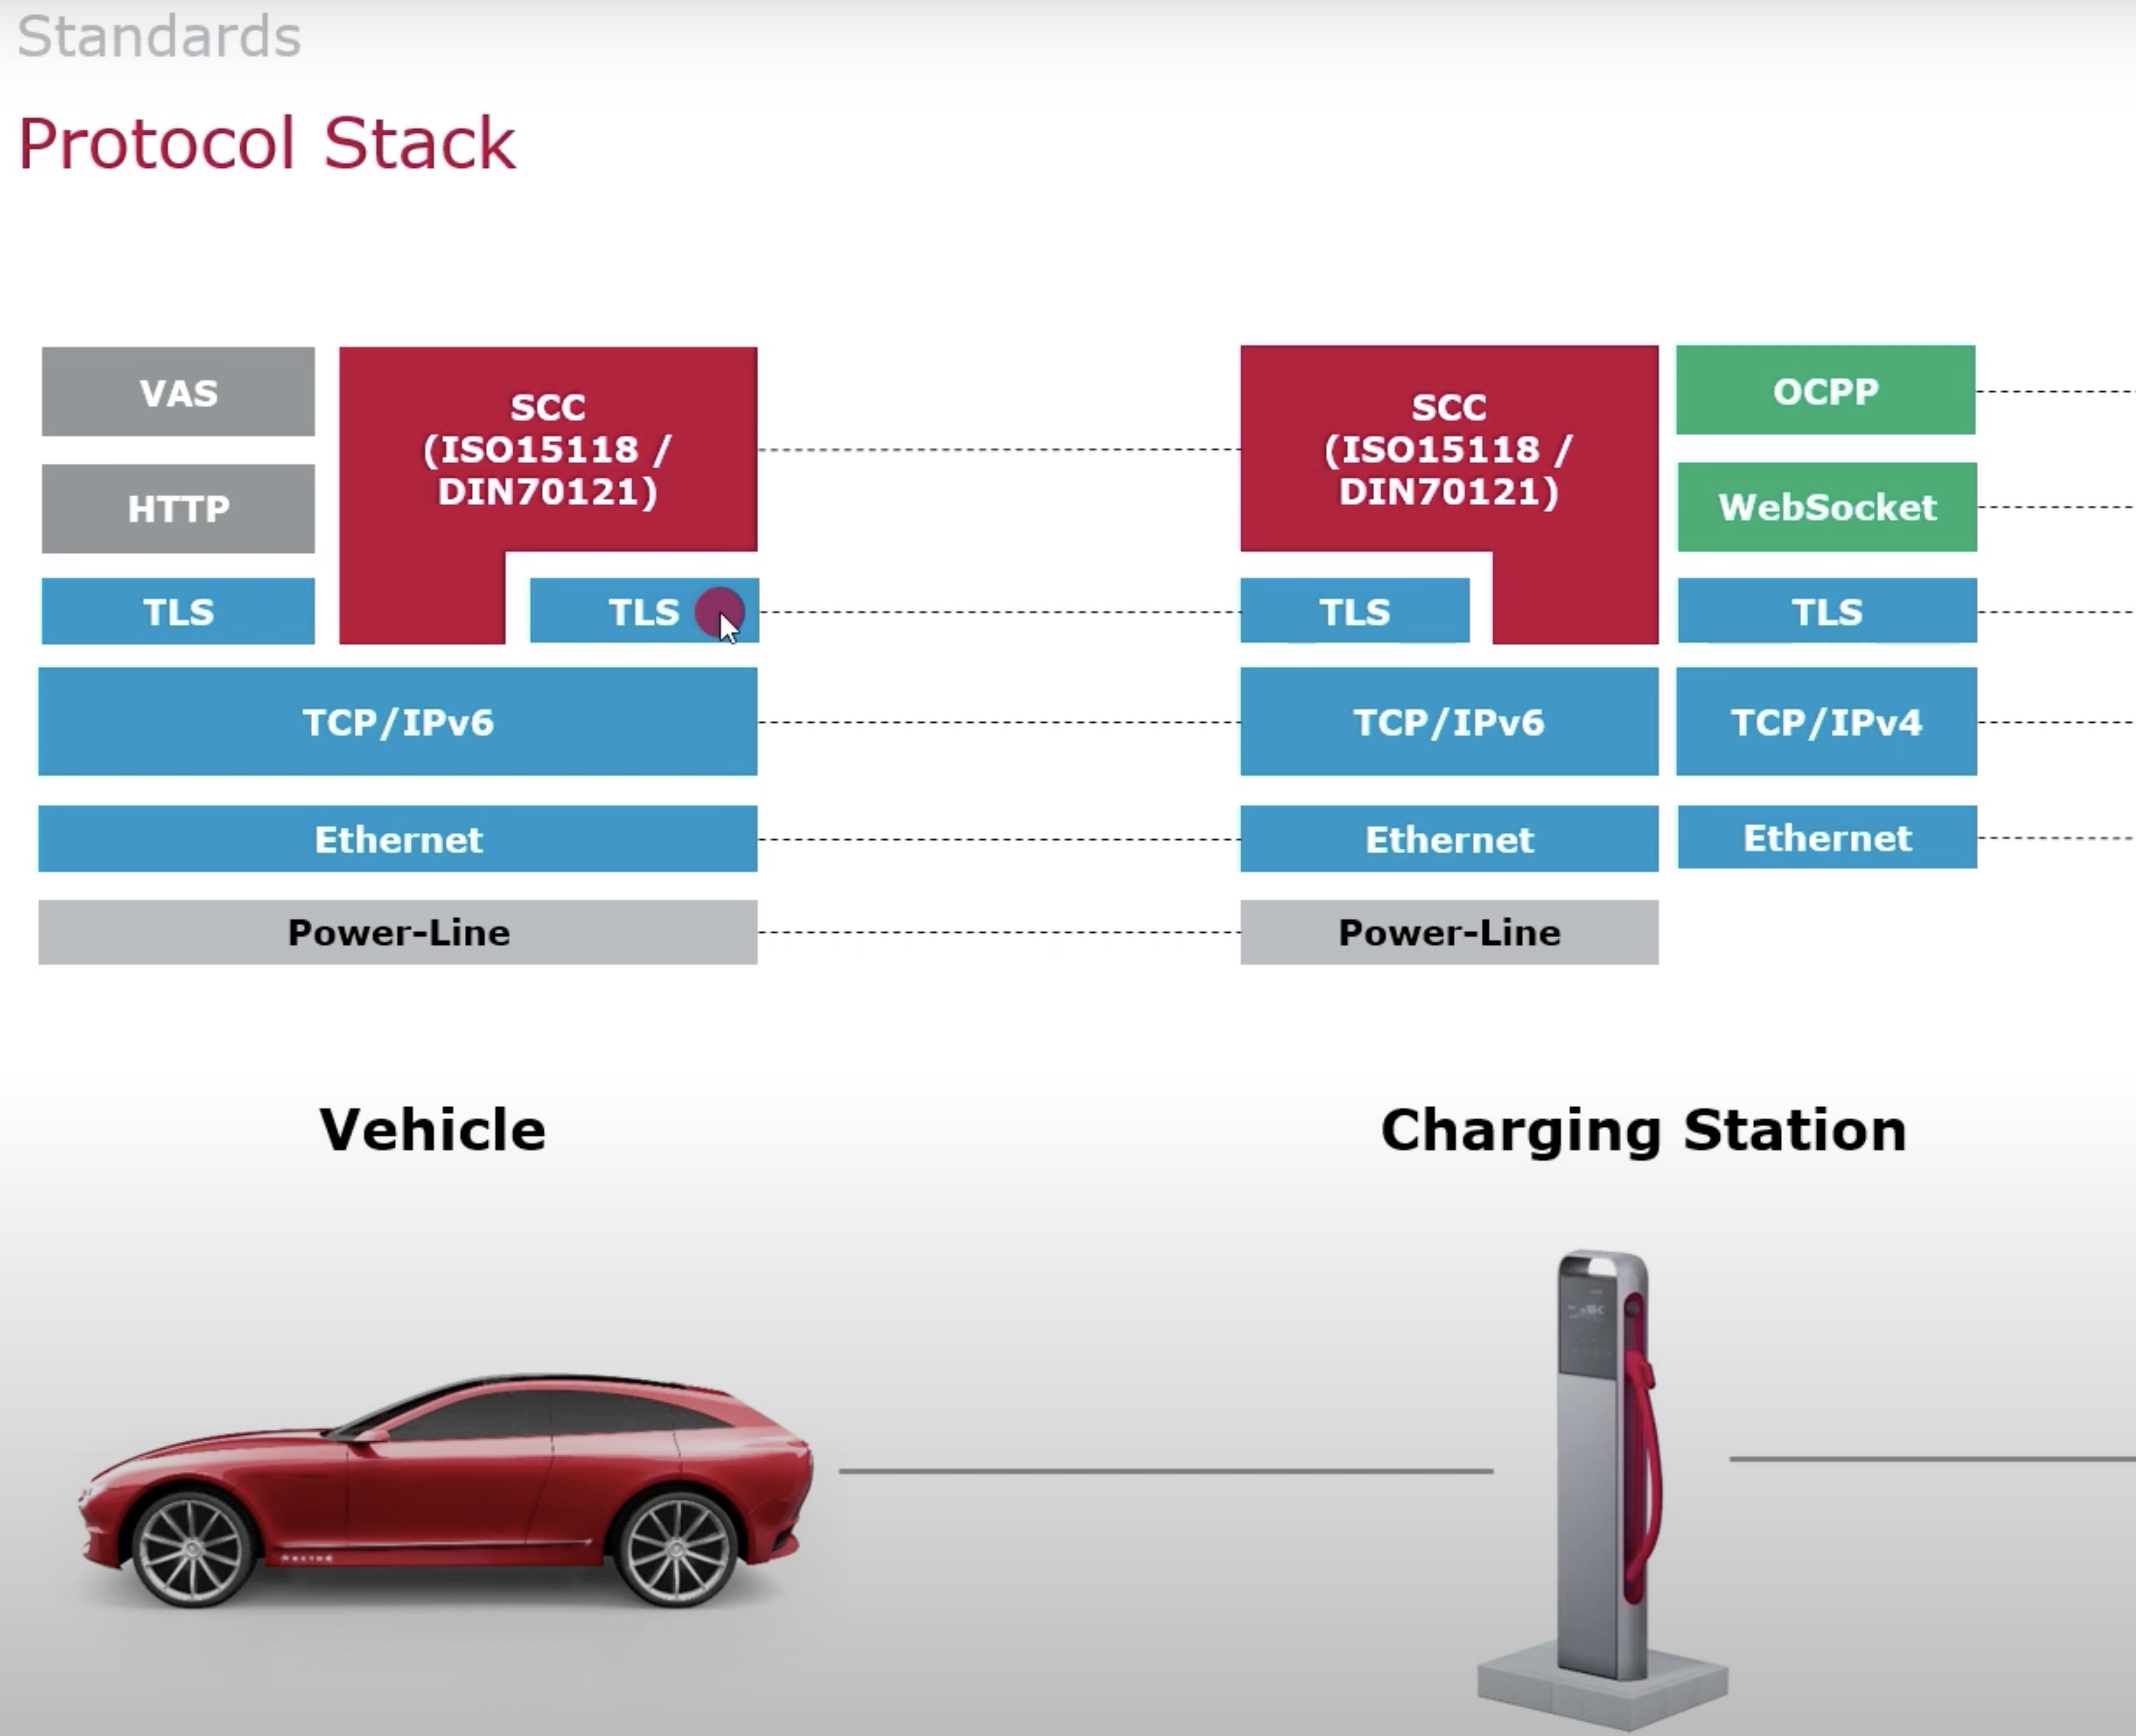
\includegraphics[width=0.6\linewidth]{images/EV_CS_Protocols.png}
    \caption[Current Electric Vehicle and Charging Station protocols]{Current Electric Vehicle and Charging Station protocols \protect \footnotemark}
    \label{fig:ev_cs_protocols}
\end{figure}

\footnotetext{\url{https://www.youtube.com/watch?v=S\_llUuyAcqs}}

\subsection{Evaluation of the General Architecture of SSI with IoT}
\label{subsec:evaluation_of_the_general_architecture}

It was evident that the Verifiable Electric Vehicle Charging System as proposed in this work is able to fulfill most of the requirements, with the ones that were not having been provided documentation in order to apply them in the future.

Despite having presented one use case of Self-Sovereign Identity with Internet of Things devices (EVs and CSs) that presents good prospects for adoption, assessing the general architecture presented on Section~\ref{subsec:architecture_for_ssi_with_iot} requires a more in-depth analysis, making use of other case studies. For this end, more use cases need to be discussed to give power to this idea. Nonetheless, it was possible to verify that in IoT devices that do not lack computational power and electricity, there are existing implementations of agents and networks that could be used by such devices, like an EV. On top of that, the general architecture presents the necessary components for any Self-Sovereign Identity system that has agents acting on behalf of any entity, whether humans, organizations, or IoT devices.



\section{Conclusion}
\label{sec:conclusion}

In this chapter the conclusions for this study are presented, by doing a summary of the study and its main contributions.
This study aimed at responding to the following research question: \textit{"What are the requirements for Self-Sovereign Identity (SSI) to be implemented effectively in an Internet of Things (IoT) environment?"}.

Towards addressing this question, in Chapter~\ref{sec:background} background information was provided on the topic of (Digital) Identity, the history of Identity Management Systems through time, and then the fundamentals of Self-Sovereign Identity were presented. The latter included mentions to Decentralized Identifiers, \textit{DIDComm}, Verifiable Credentials, Wallets, Agents, etc. Still in this chapter, the related work was presented, where it was evident that the field of Self-Sovereign Identity with IoT is not yet mature, but provided much information on the advantages of a blockchain-based IdMS. Much of the literature on SSI with IoT provided an analysis on the current state of technologies and solutions available for that purpose, from which a comparison was made, to understand the differences between them.

Chapter~\ref{sec:requirement_elicitation} narrowed the field of research from SSI with IoT to the automotive domain and more specifically to the Electric Vehicle Charging use case. Here the current state of Electric Vehicle Charging Networks was presented. The use case was analyzed with the assistance of domain experts, from which the major liabilities were extracted, alongside a set of requirements with regards to the necessary settlements between the different parties in order for the owner of an EV to be able to charge its vehicle. 

In Chapter~\ref{section:design_and_implementation} the system design was presented, where the architecture of a novel Verifiable Electric Vehicle Charging network architecture was presented, based on a set of technological decisions taken at the beginning of that same chapter that would facilitate the largest number of requirements. Afterwards, the system was analyzed with regards to the changes needed in the original flow of interactions, to accommodate for the SSI-driven approach.

Chapter~\ref{sec:implementation_and_deployment_details} outlined the necessary steps used to implement the system and how to deploy it. The system consists of a dockerized full stack application that is able to interact with the agents and perform custom actions tailored for the particular use case at hand. 

In Chapter~\ref{section:evaluation} the assessment of the system was made, through means of benchmarks, questionnaires made to domain experts and cross-checking the requirements with decisions taken across this study. The overall assessment was positive given that almost all requirements were met, and the ones that were not fulfilled were discussed and their fulfillment should be achievable if the measures listed are addressed in the future.
Regarding the evaluation of the general SSI with IoT research question, a step has been taken which makes that prospect possible in a near future, but more use cases need to be investigated to determine more limitations and explore different IoT devices, for example sensors, home assistants, or others.

\newpage

\section{Future Work}
\label{subsec:future_work}

In this chapter future work is sketched in order to provide more solidity to the claims made in the tackled use case (Verifiable Electric Vehicle Charging) and to validate the general case of SSI with IoT.

\subsection*{Experiment with other DLTs}
\label{subsubsec:experiment_with_other_dlts}

Given that the decision to opt for Hyperledger Indy for the DLT was taken largely due to its active community and public availability, in detriment of the IOTA Tangle approach or any of the others listed in Section~\ref{subsec:existing_technologies_and_application_domains}, it would be interesting to assess the differences in the implementation whether a different DLT was adopted. Possibly with the IOTA Tangle users would have a more scalable solution, which might address Requirement~\ref{evaluation:NFR-1.1} that was marked as inconclusive with the Hyperledger Indy approach.

\subsection*{Investigate with other use cases}
\label{subsubsec:investigate_with_other_use_cases}

As mentioned at the end of Chapter~\ref{section:evaluation}, assessing more use cases is crucial to understanding the possibilities of incorporating SSI with IoT. This project focuses on IoT devices that fortunately do not lack any computational power or electricity, which is an assumption that cannot be made for all IoT devices. Therefore it is imperative to study how SSI could be enabled for low-capacity IoT devices to be able to respond with more certainty to the presented research question.

\subsection*{Merge proof requests}
\label{subsubsec:merge_proof_requests}

Although a small improvement to the system, it would be interesting to assess the feasibility of merging two or more credential requests into a single presentation request, in order to minimize user interactions with the system, as required by Requirement~\ref{evaluation:FR-3.4}.

\subsection*{Address GDPR compliance and other limitations}
\label{subsubsec:address_gdpr_compliance}

One of the pending matters of this project is the fact that, given the fact that it was built on top of a proof-of-concept, privacy concerns in the proposed solution were simplified, leaving room for linkability between the EV Owner and its EV. This has been addressed as a limitation in the Evaluation chapter (Section~\ref{subsubsec:limitations}), and in order to account for these liabilities, it is necessary to create means to link the EV Owner with its EV using a mechanism different than the usage of a unique identifier between the two. A possible approach would be to generate a different number every session so that the link between the two could not be established by the Charging Station, but the feasibility of this mechanism can be a topic for a thesis of its own. The remaining of the limitations also need to be cleared in order to think about applying this solution to a prototype/production level application.


\pagestyle{contents}

\bibliographystyle{ieeetr}
\bibliography{biblio}

\pagestyle{appendix}
\appendix
\section*{Appendices}
\addcontentsline{toc}{section}{Appendices}
\renewcommand{\thesubsection}{\Alph{subsection}}

\subsection{How to Install Trinsic Wallet Agent Mobile Application}
\label{app:trinsic_installation}

The process of installing and setting up the Trinsic Wallet Agent depends on the operating system, with the application being available on both Apple's App Store and also Android's Google Play Store. During this project the Android version was used and that is the version that will be explained below.

\begin{itemize}
    \item Navigate to the desired Store and download the Trinsic Wallet App. Either Google Play Store\footnote{\url{https://play.google.com/store/apps/details?id=id.streetcred.apps.mobile}} or Apple's App Store\footnote{\url{https://apps.apple.com/us/app/trinsic-wallet/id1475160728}}.
    \item Follow the in-app instructions to setup a wallet.
    \item Follow the instructions on Figures~\ref{fig:trinsic_1}, \ref{fig:trinsic_2} and \ref{fig:trinsic_3} to change to the same network as the ACA-Py agents.
\end{itemize}

\begin{figure}[!htb]
\minipage{0.32\textwidth}
  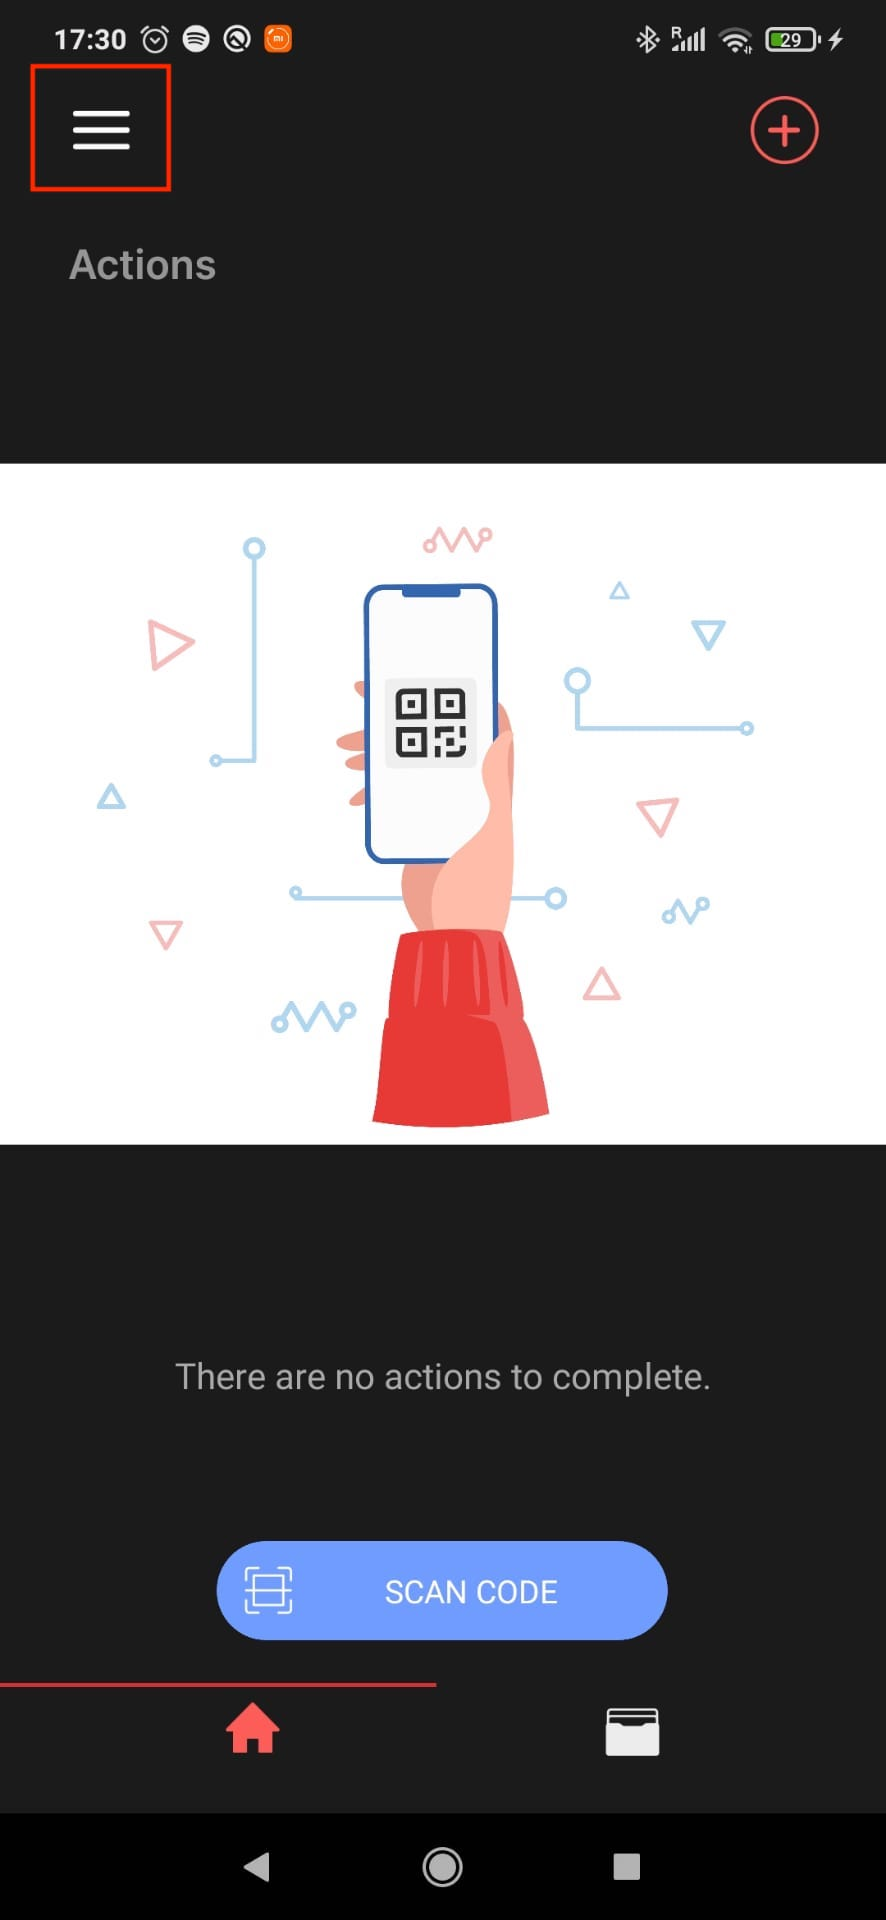
\includegraphics[width=\linewidth]{images/Trinsic/Trinsic_welcome_screen.jpeg}
  \caption[]{Go to Settings}\label{fig:trinsic_1}
\endminipage\hfill
\minipage{0.32\textwidth}
  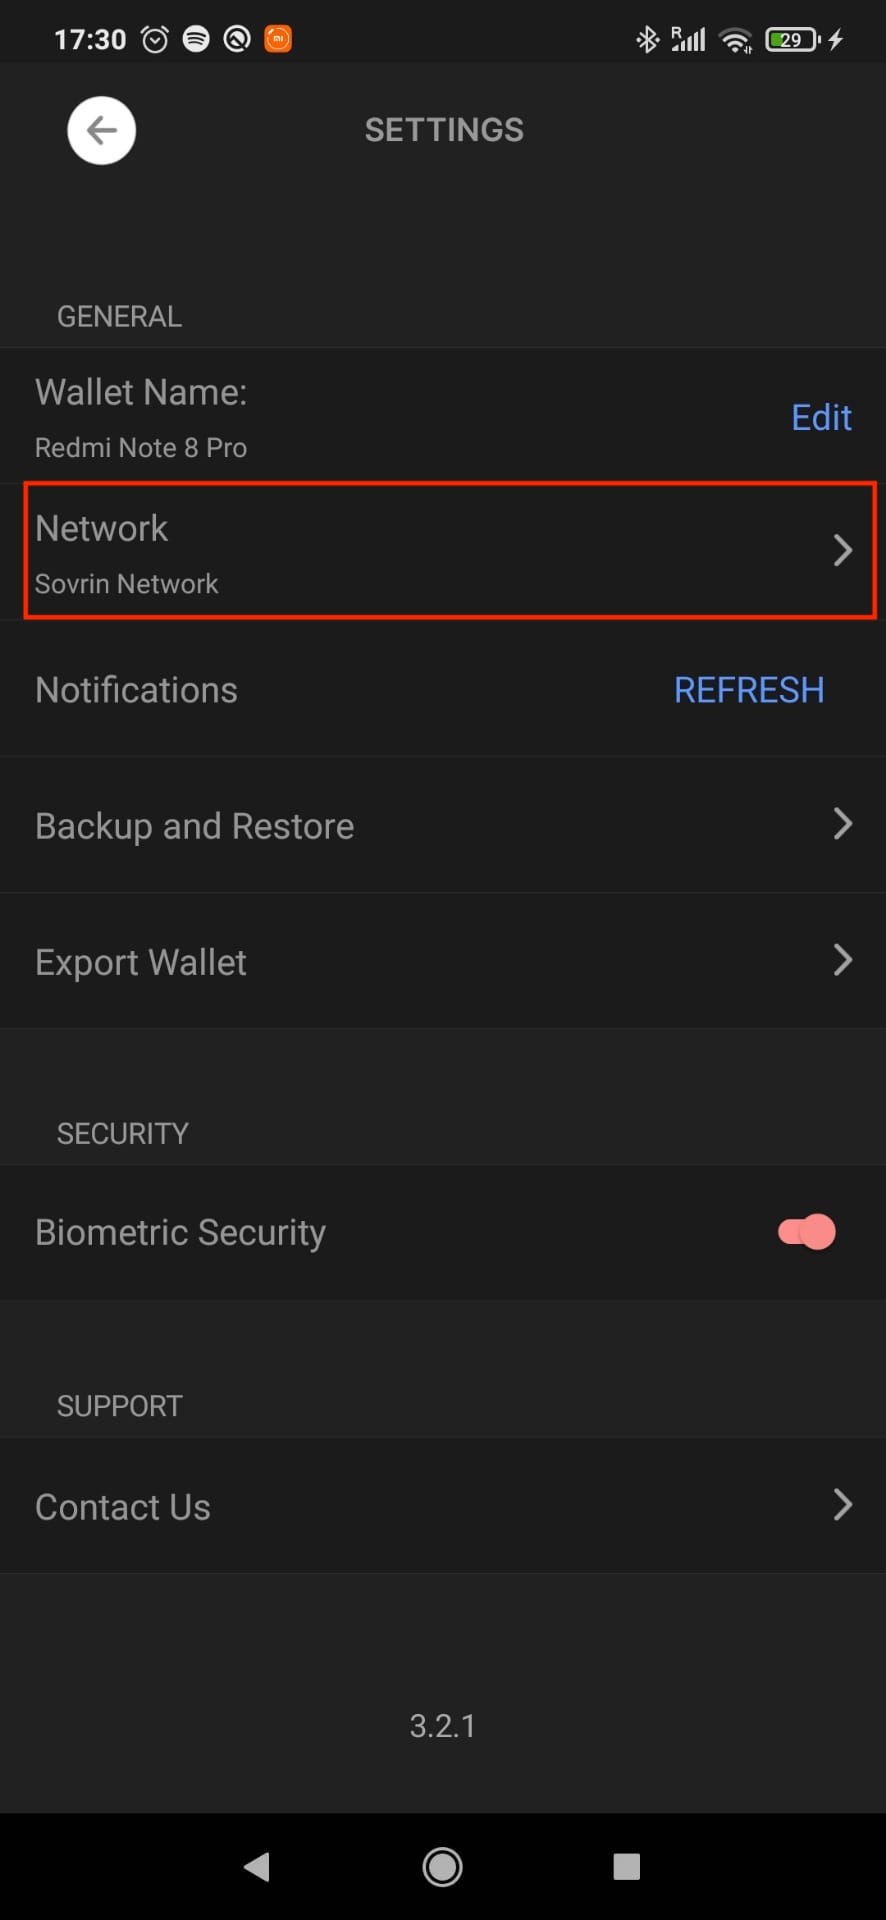
\includegraphics[width=\linewidth]{images/Trinsic/Trinsic_setup_network1.jpeg}
  \caption[]{Choose "Network" Option}\label{fig:trinsic_2}
\endminipage\hfill
\minipage{0.32\textwidth}%
  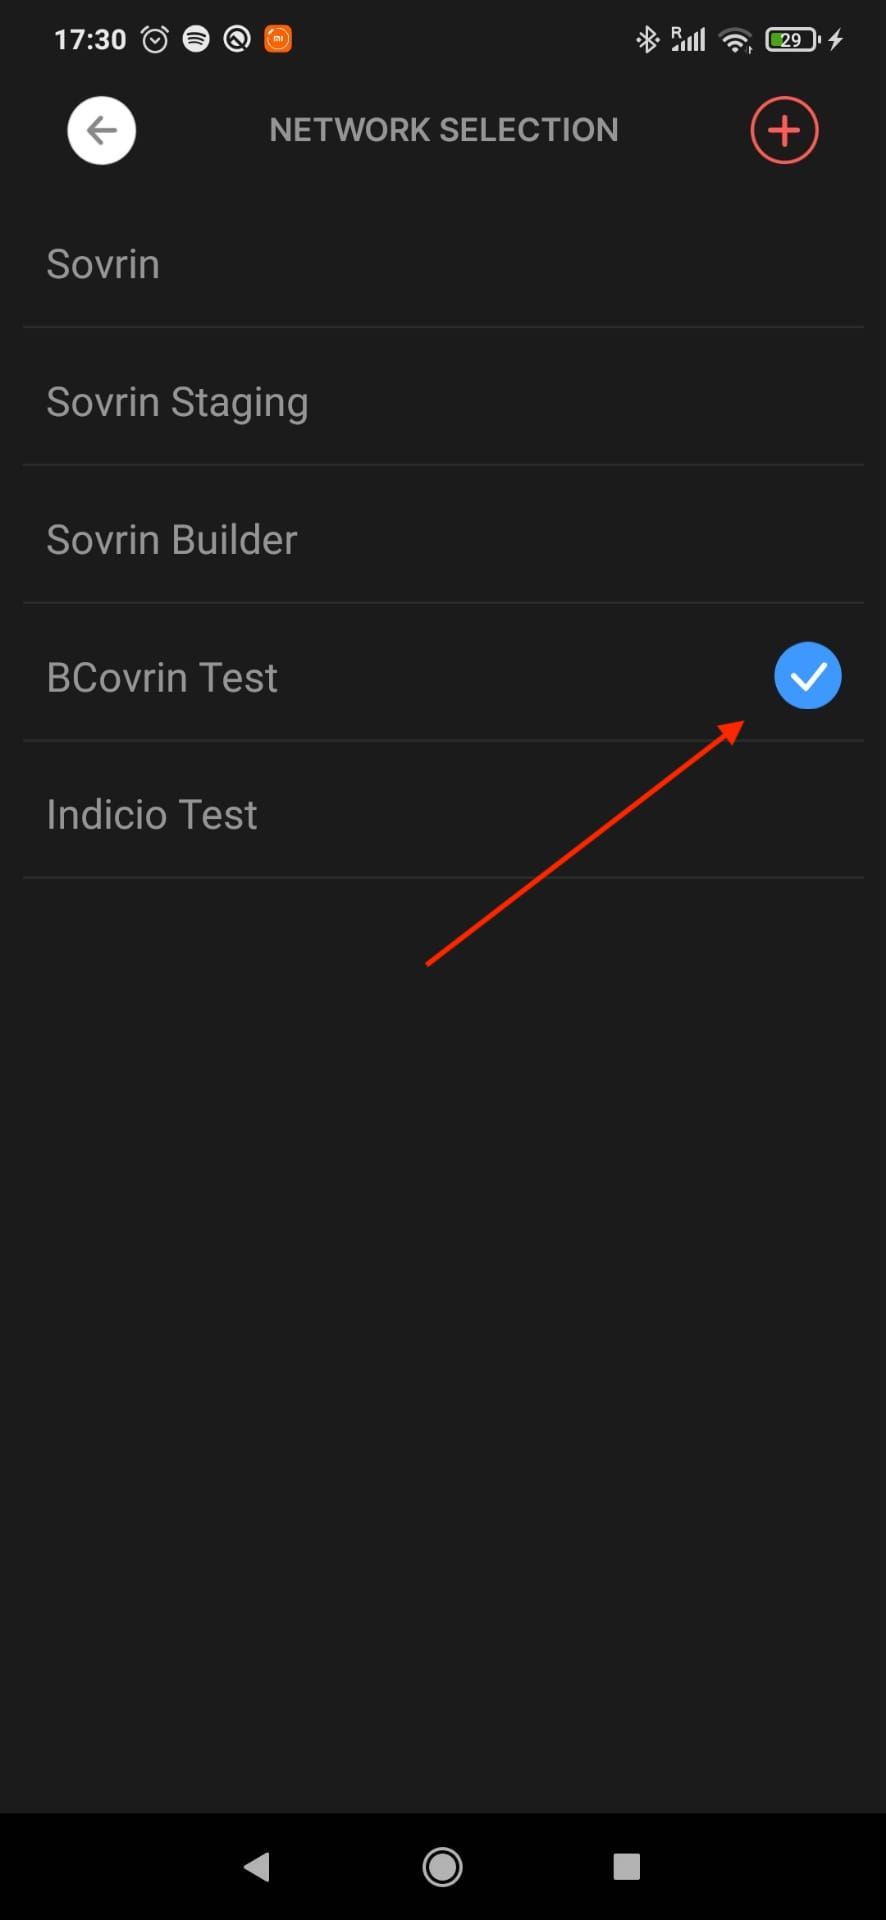
\includegraphics[width=\linewidth]{images/Trinsic/Trinsic_setup_network2.jpeg}
  \caption[]{Change it to "BCovrin Test"}\label{fig:trinsic_3}
\endminipage
\end{figure}

\newpage    % I wanted each new appendix to start on a new page

\subsection{Application Screenshots}
\label{app:application_screenshots}

In this appendix the screenshots of the frontend as well as from the Trinsic Wallet App on the EV Owner's phone are presented, to illustrate each step of each use-case.

\subsubsection{Service Providers Flow with SSI Screenshots}
\label{subapp:service_providers_flow}

\begin{figure}[H]
    \centering
    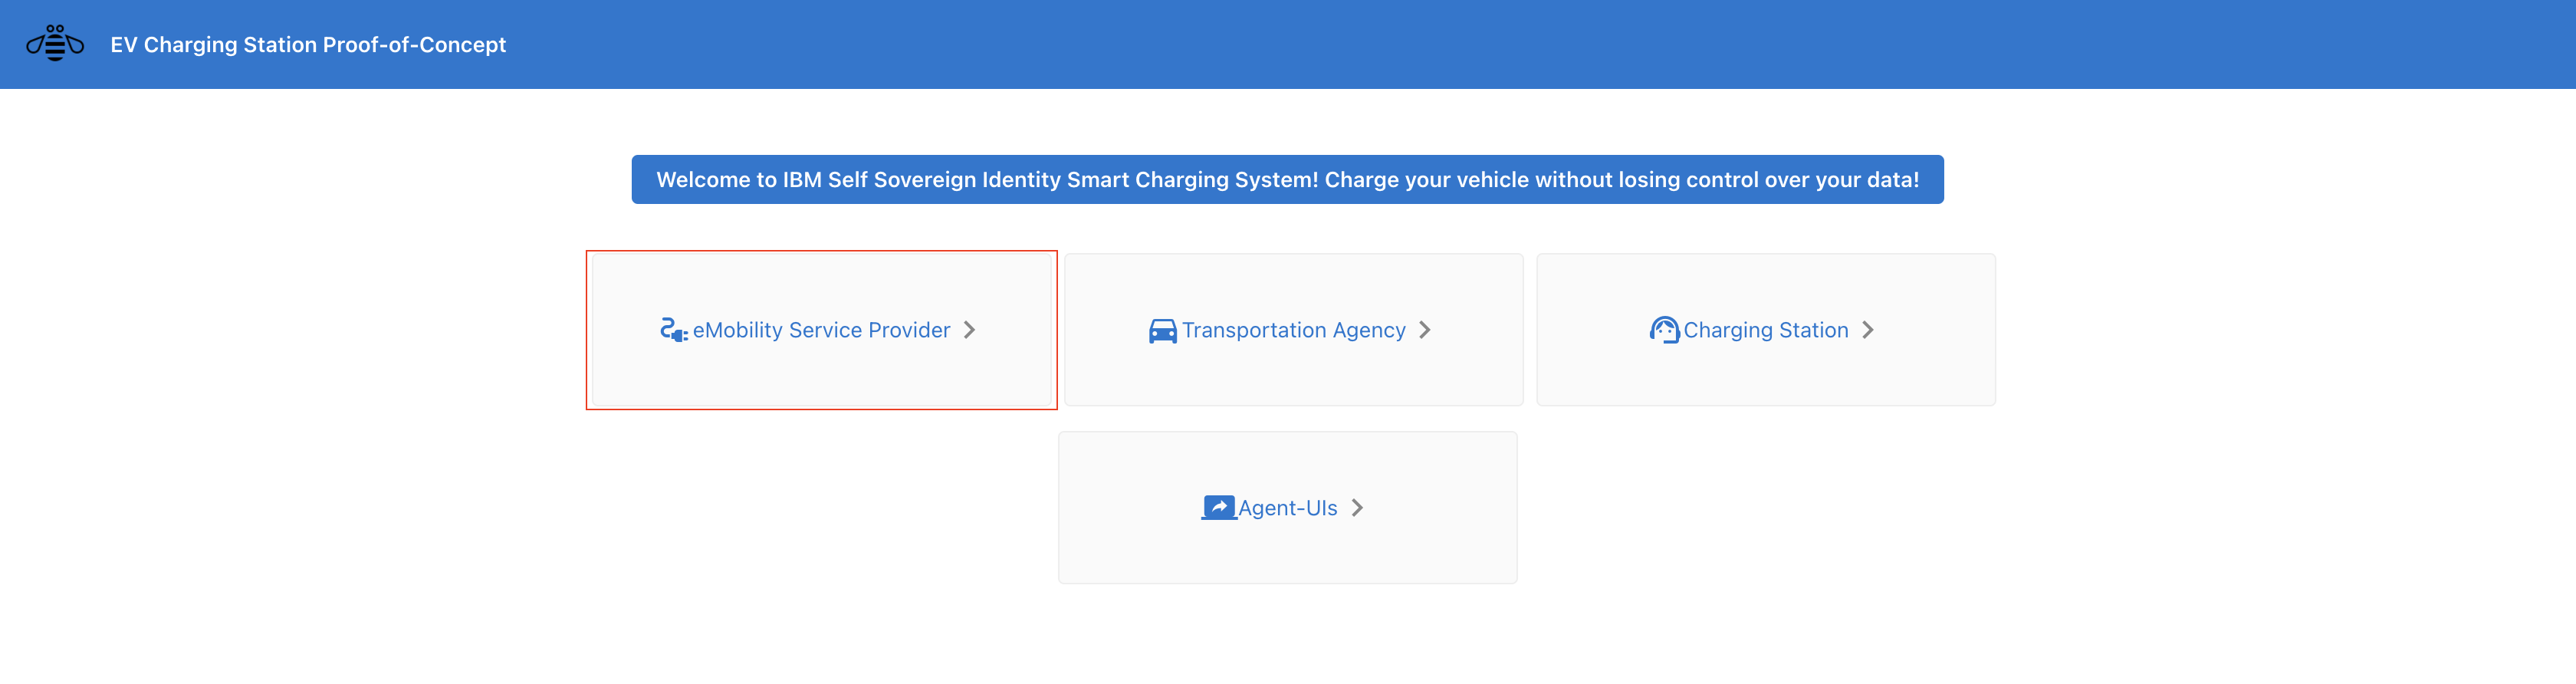
\includegraphics[width=\linewidth]{images/Frontend/eMSP/Screenshot1.png}
    \caption[]{Selecting eMSP portal}
    \label{fig:service_provider_screenshot_1}
\end{figure}

\begin{figure}[H]
\centering
\begin{minipage}{.5\textwidth}
  \centering
  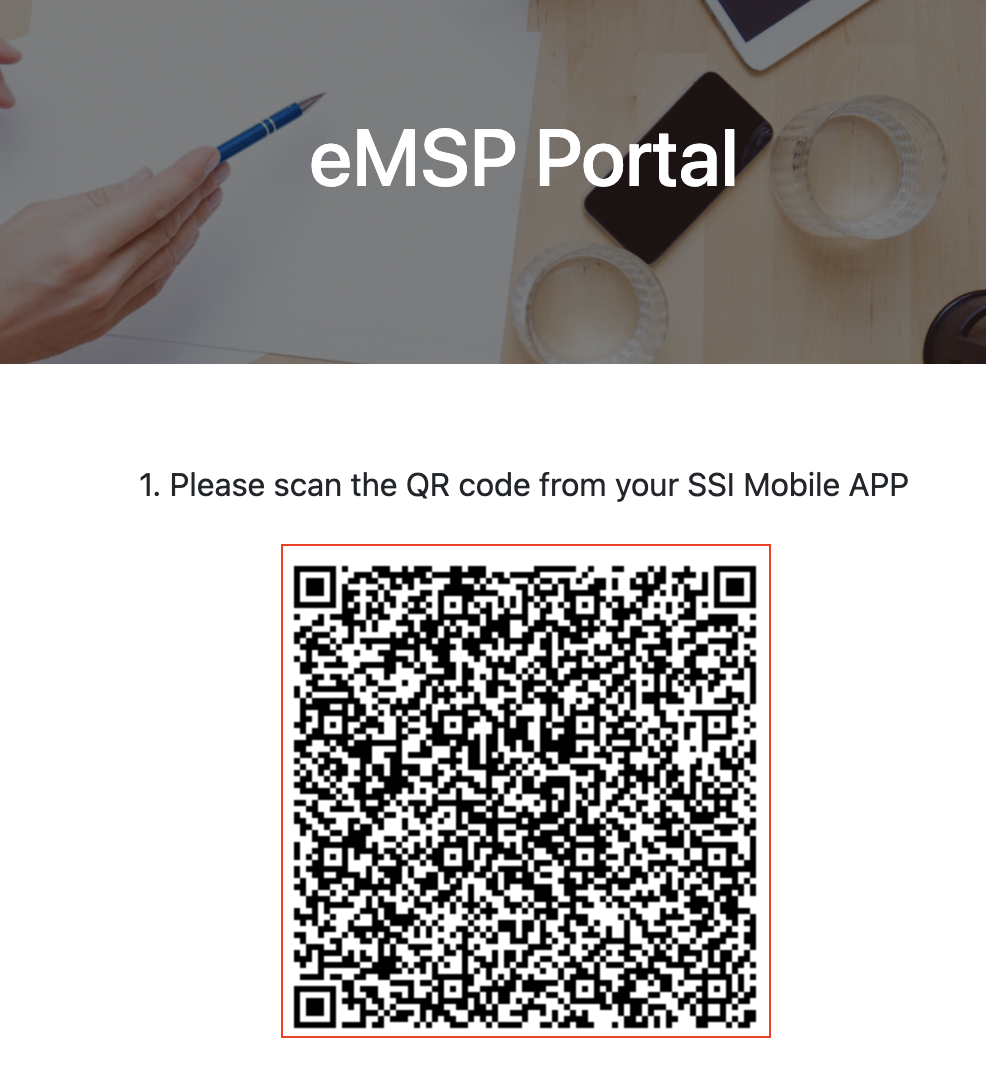
\includegraphics[width=.8\linewidth]{images/Frontend/eMSP/Screenshot2.png}
  \caption[]{Connect to eMSP Agent using QR Code}
  \label{fig:service_provider_screenshot_2}
\end{minipage}%
\begin{minipage}{.5\textwidth}
  \centering
  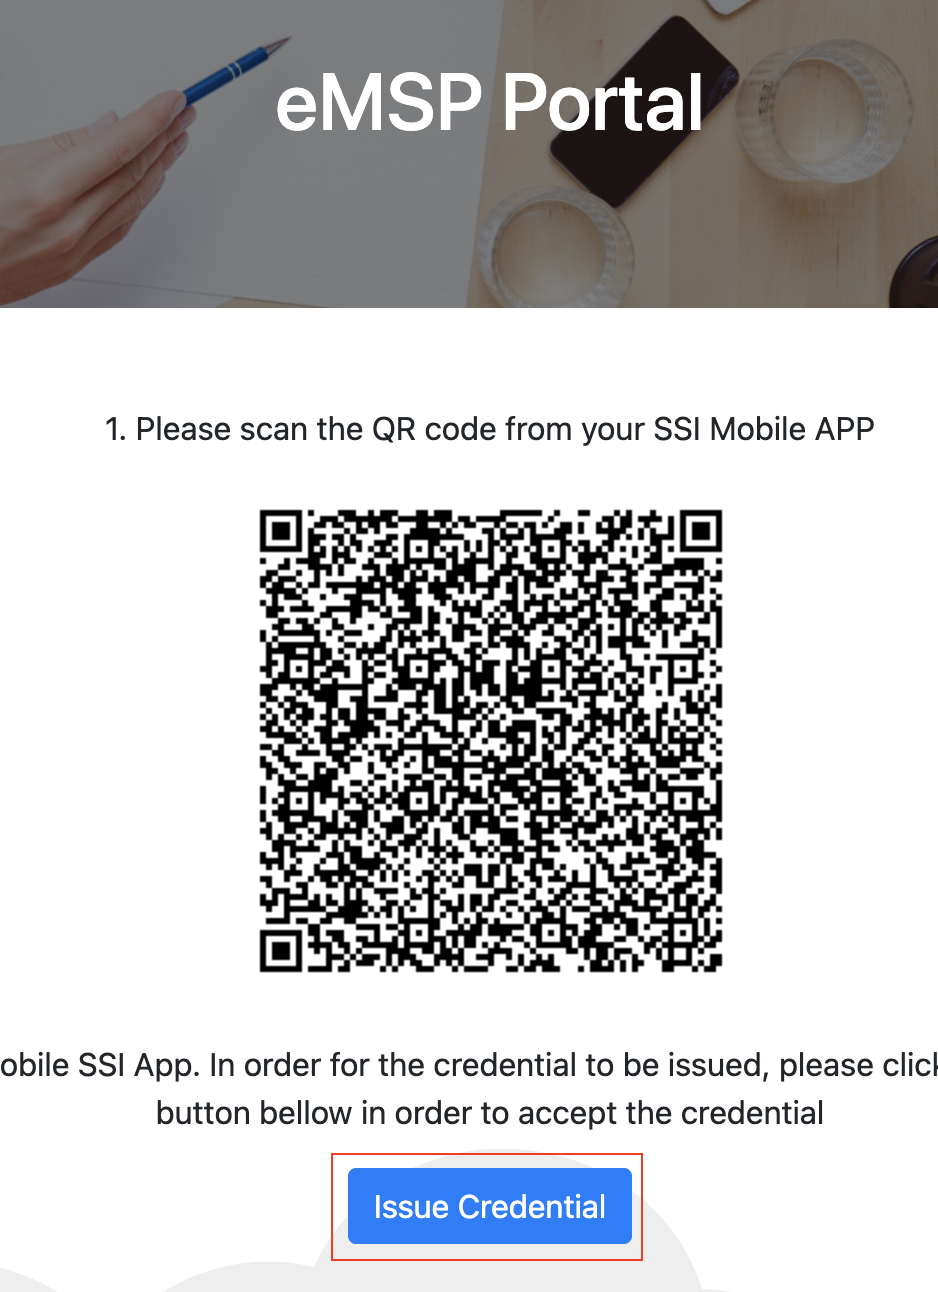
\includegraphics[width=.8\linewidth]{images/Frontend/eMSP/Screenshot3.png}
  \caption[]{Press the "Issue Credential" button}
  \label{fig:service_provider_screenshot_3}
\end{minipage}
\end{figure}

\begin{figure}[H]
    \centering
    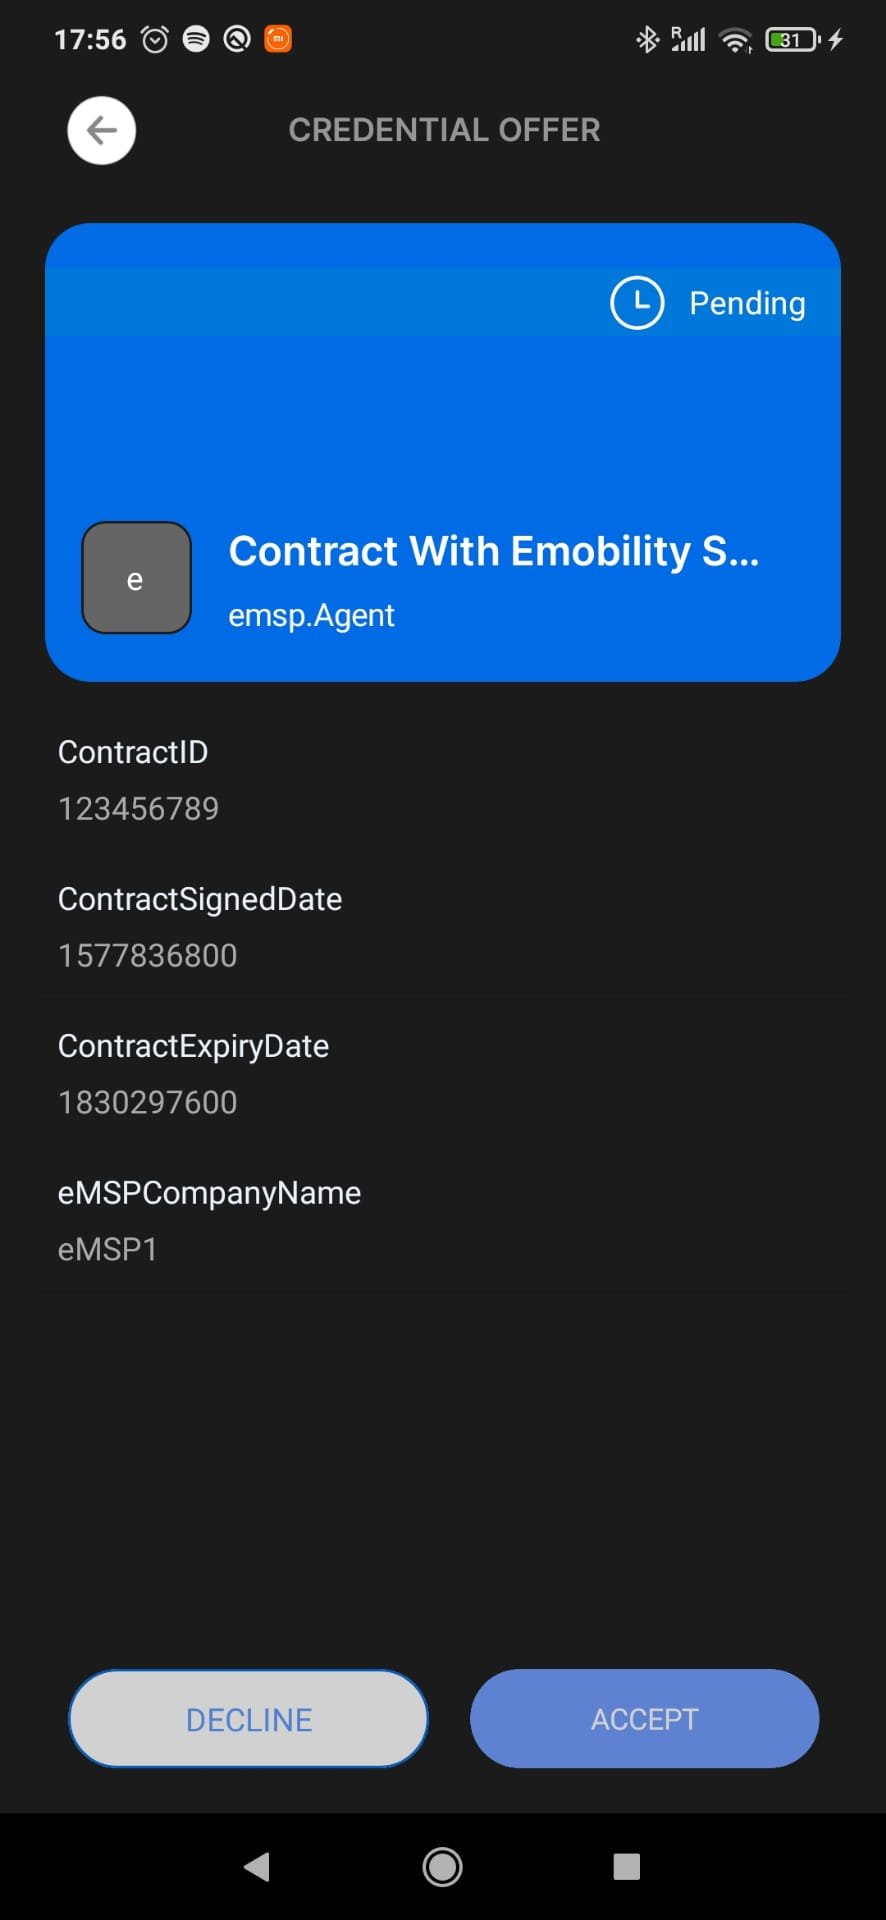
\includegraphics[width=0.4\linewidth]{images/Frontend/eMSP/Screenshot4.jpeg}
    \caption[]{Accept the credential on the Trinsic Wallet App}
    \label{fig:service_provider_screenshot_4}
\end{figure}

\newpage

\subsubsection{EV Owner and EV Interactions with SSI Screenshots}
\label{subapp:ev_owner_and_ev_interactions}

\begin{figure}[H]
    \centering
    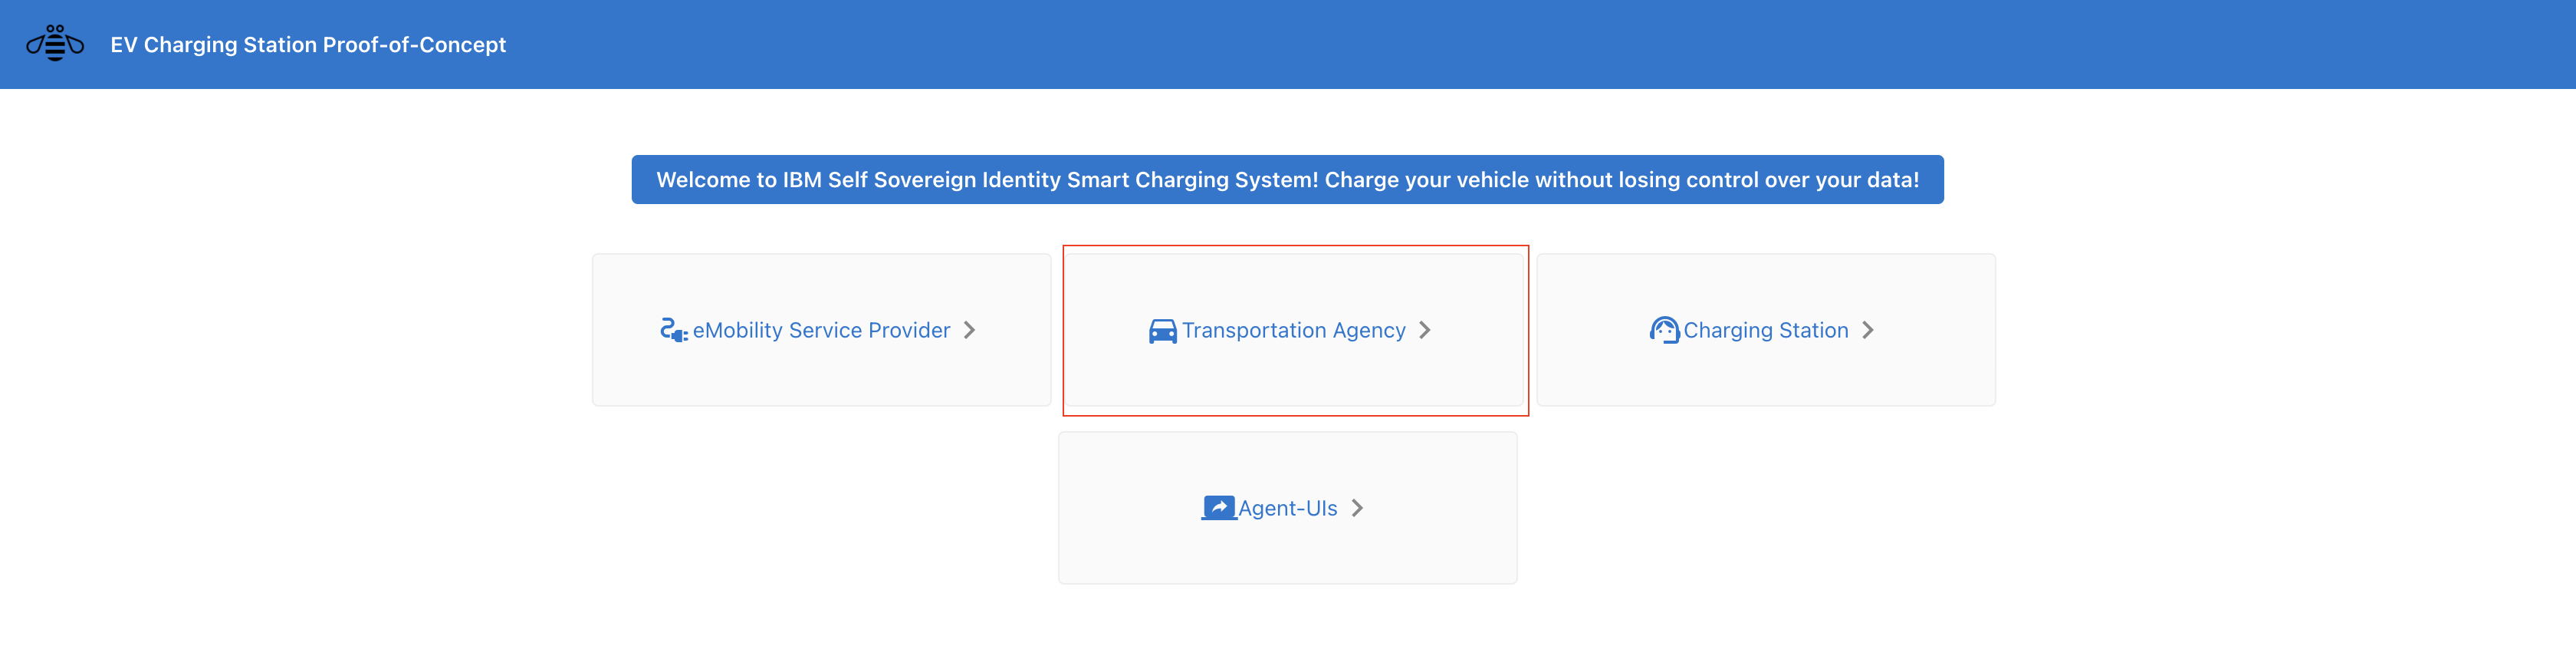
\includegraphics[width=\linewidth]{images/Frontend/Transportation_agency/Screenshot1.png}
    \caption[]{Selecting Transportation Agency portal}
    \label{fig:ev_owner_screenshot_1}
\end{figure}

\begin{figure}[H]
\centering
\begin{minipage}{.5\textwidth}
  \centering
  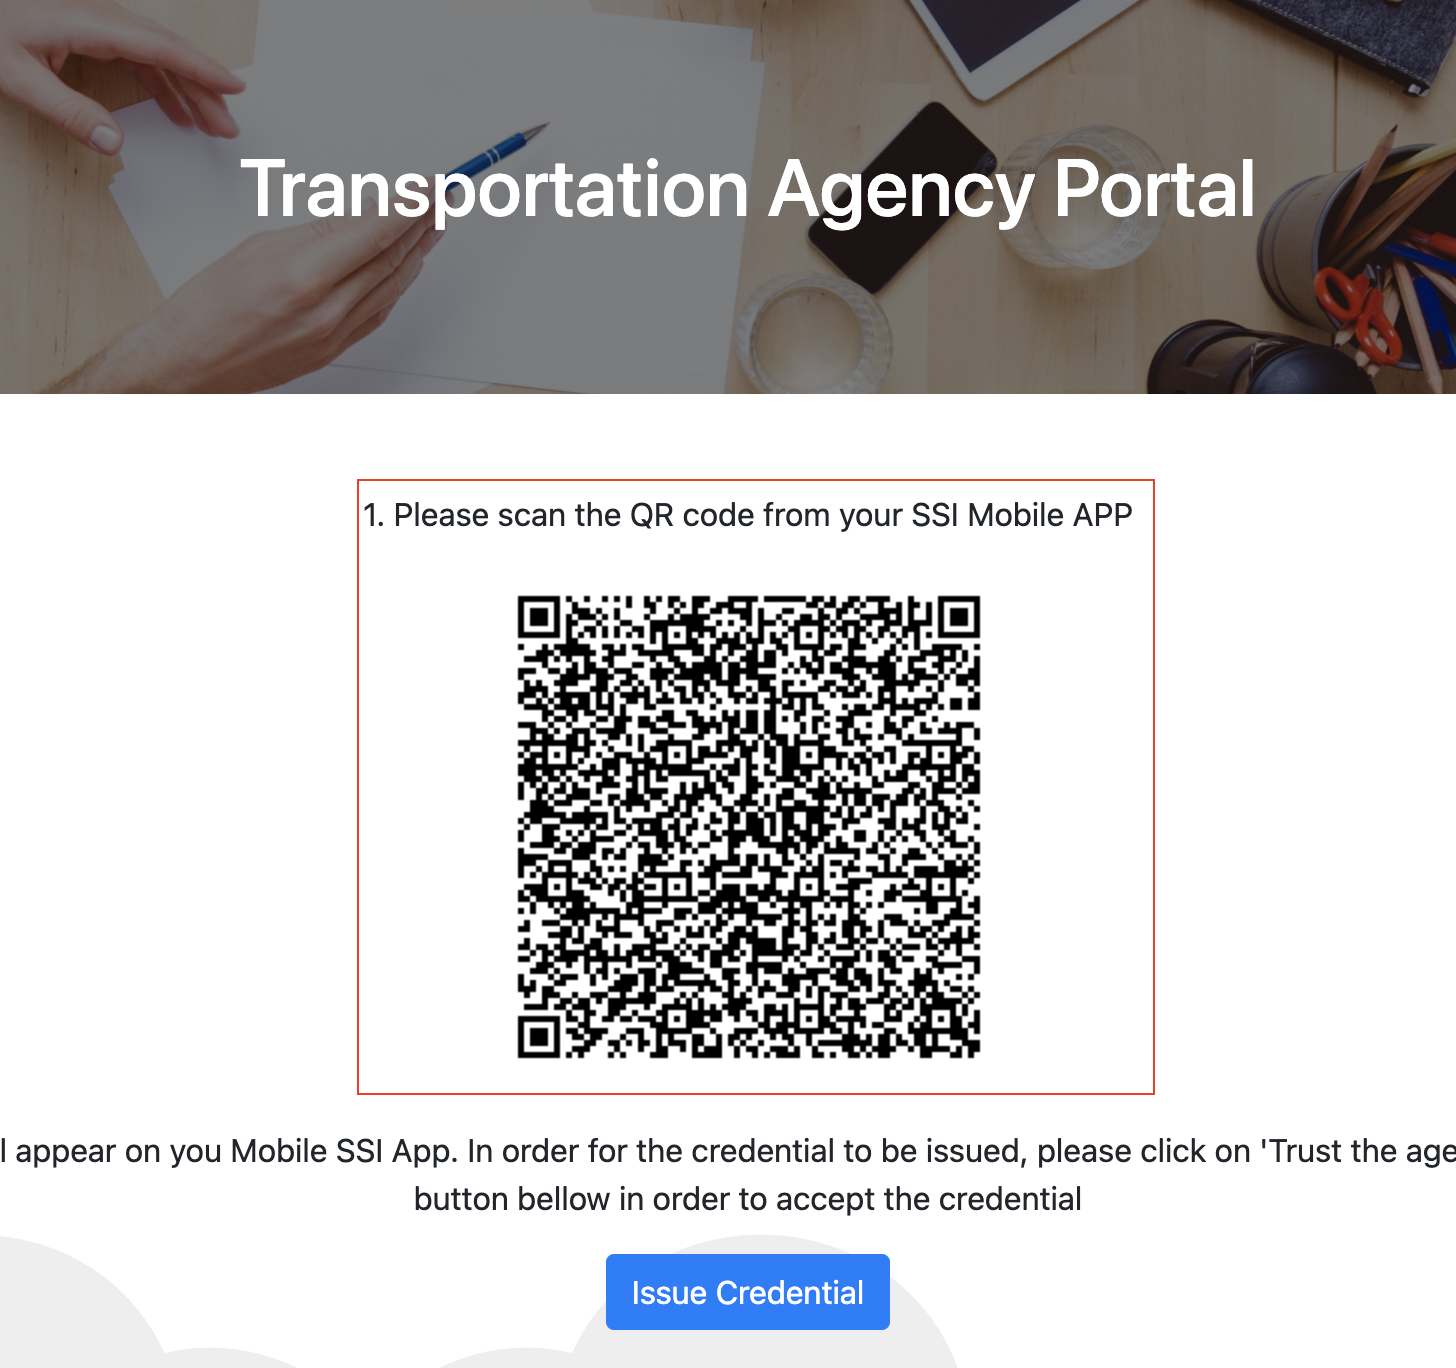
\includegraphics[width=.8\linewidth]{images/Frontend/Transportation_agency/Screenshot2.png}
  \caption[]{Connect to Transportation Agency Agent using QR Code}
  \label{fig:ev_owner_screenshot_2}
\end{minipage}%
\begin{minipage}{.5\textwidth}
  \centering
  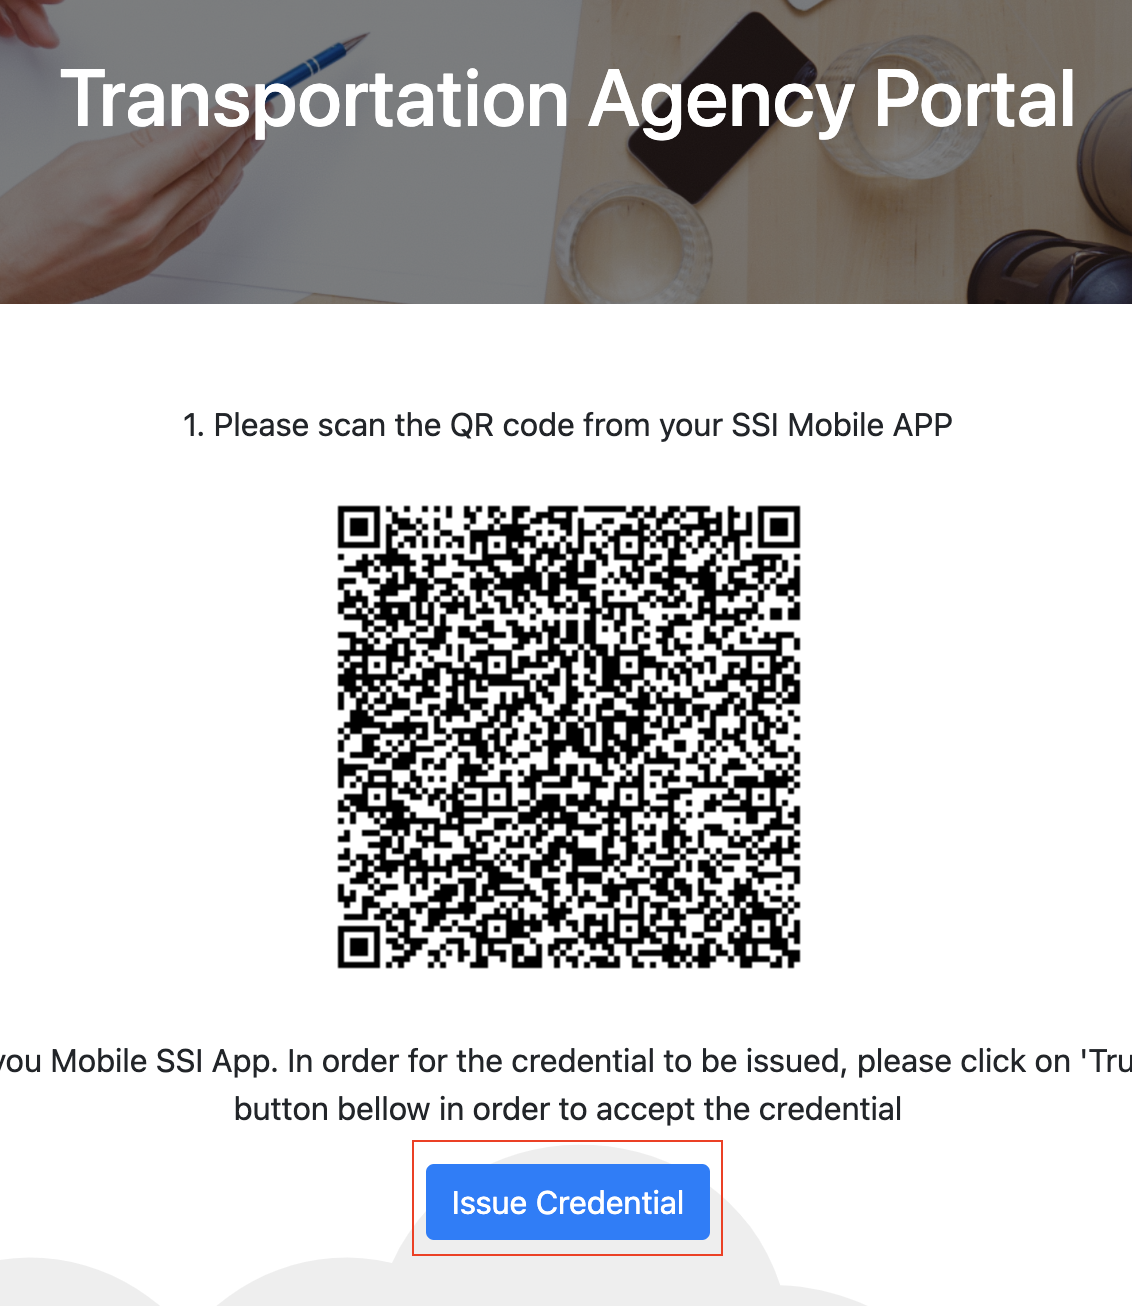
\includegraphics[width=.8\linewidth]{images/Frontend/Transportation_agency/Screenshot3.png}
  \caption[]{Press the "Issue Credential" button}
  \label{fig:ev_owner_screenshot_3}
\end{minipage}
\end{figure}

\begin{figure}[H]
    \centering
    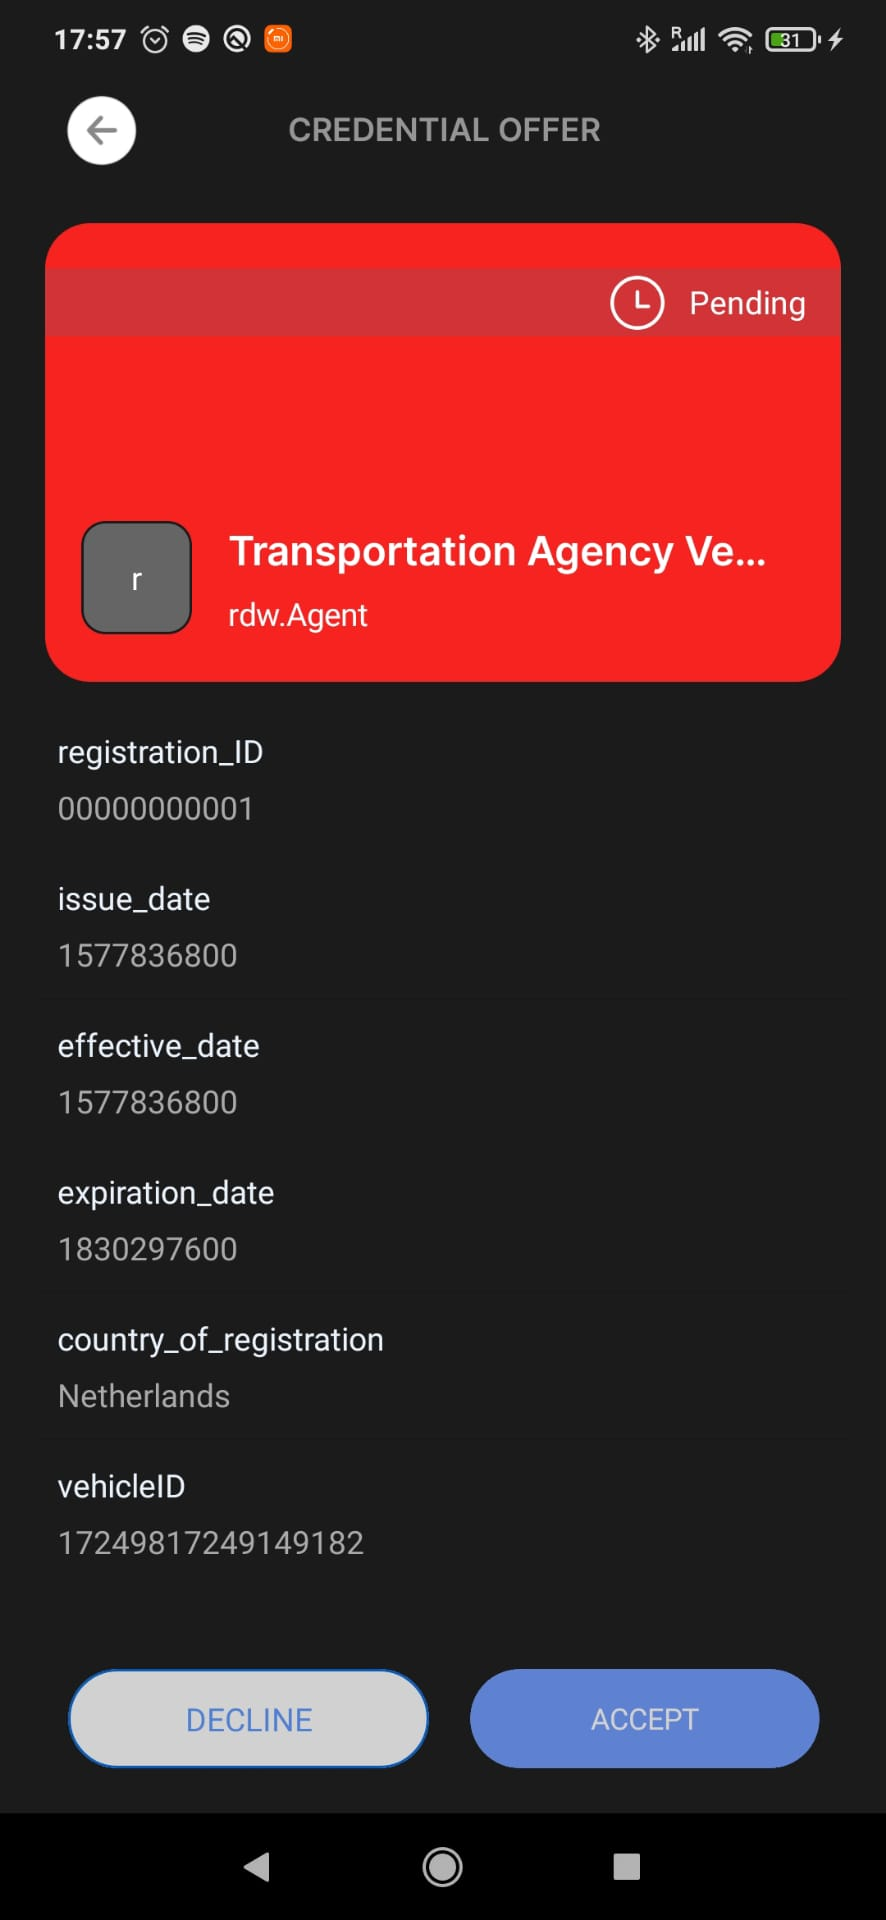
\includegraphics[width=0.4\linewidth]{images/Frontend/Transportation_agency/Screenshot4.jpeg}
    \caption[]{Accept the credential on the Trinsic Wallet App}
    \label{fig:ev_owner_screenshot_4}
\end{figure}

\newpage

\subsubsection{Charging and Billing with SSI Screenshots}
\label{subapp:charging_and_billing}

\begin{figure}[H]
    \centering
    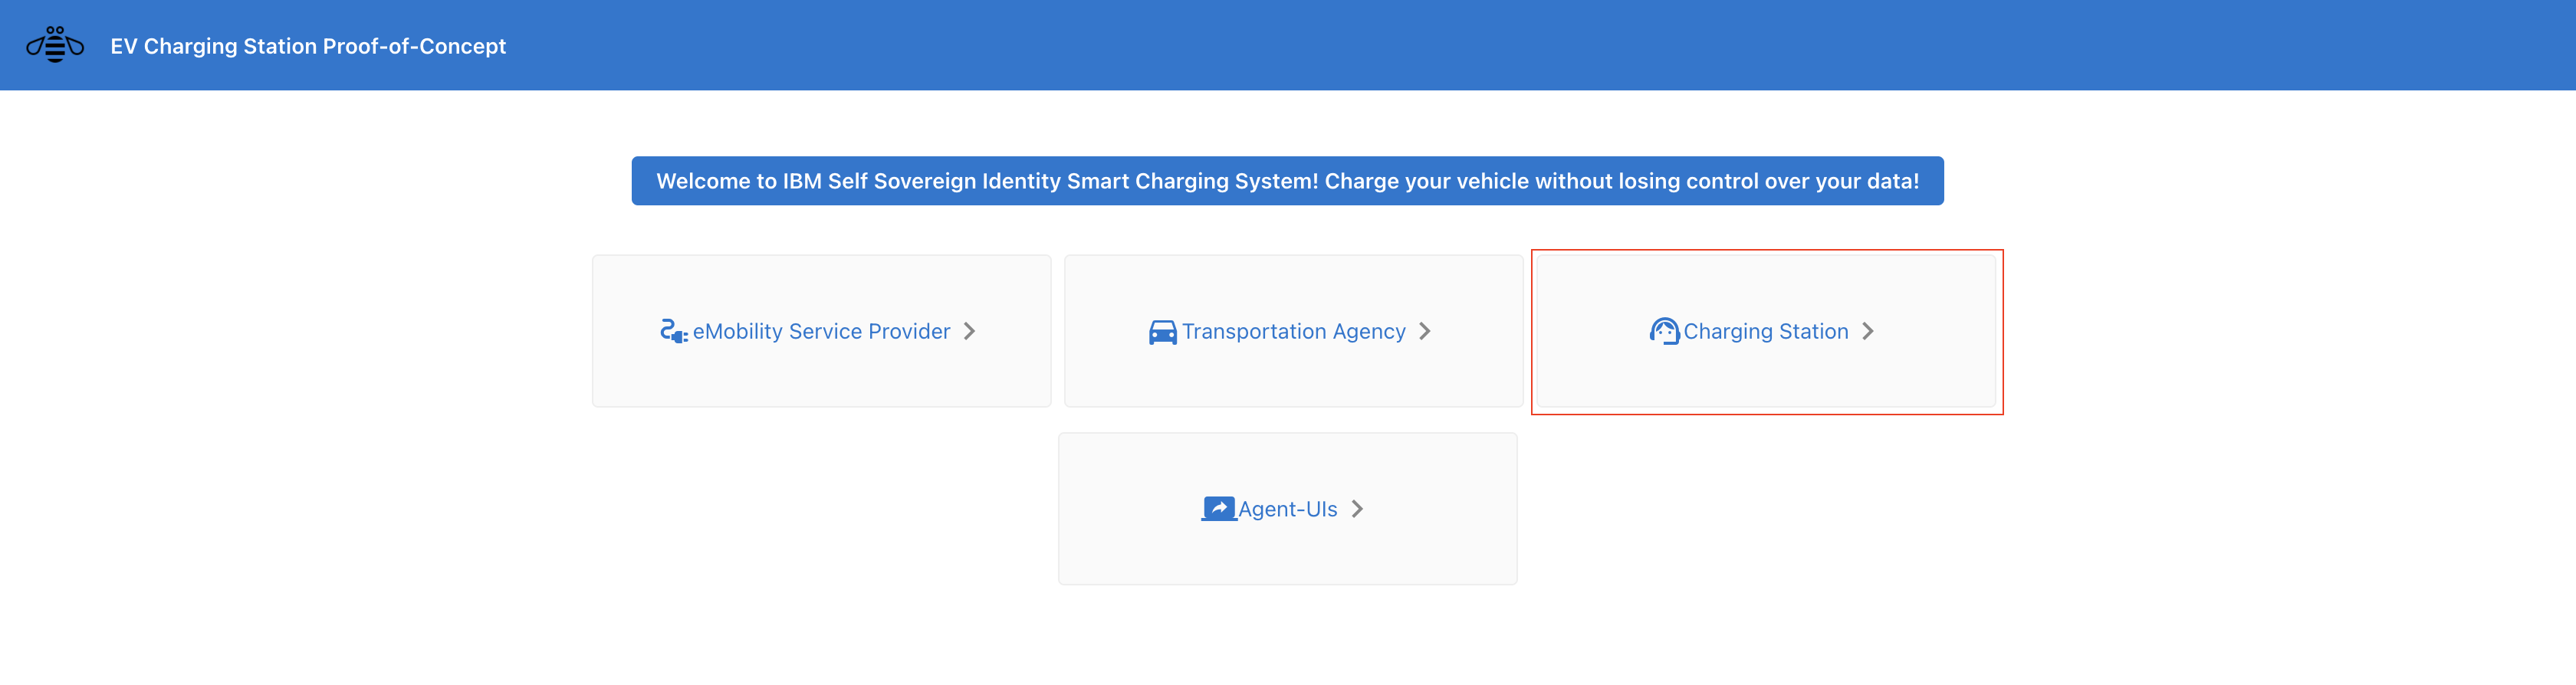
\includegraphics[width=\linewidth]{images/Frontend/Charging/1.0.png}
    \caption[]{Selecting Charging Station dashboard}
    \label{fig:charging_screenshot_1.0}
\end{figure}

\begin{figure}[H]
\centering
\begin{minipage}{.5\textwidth}
  \centering
  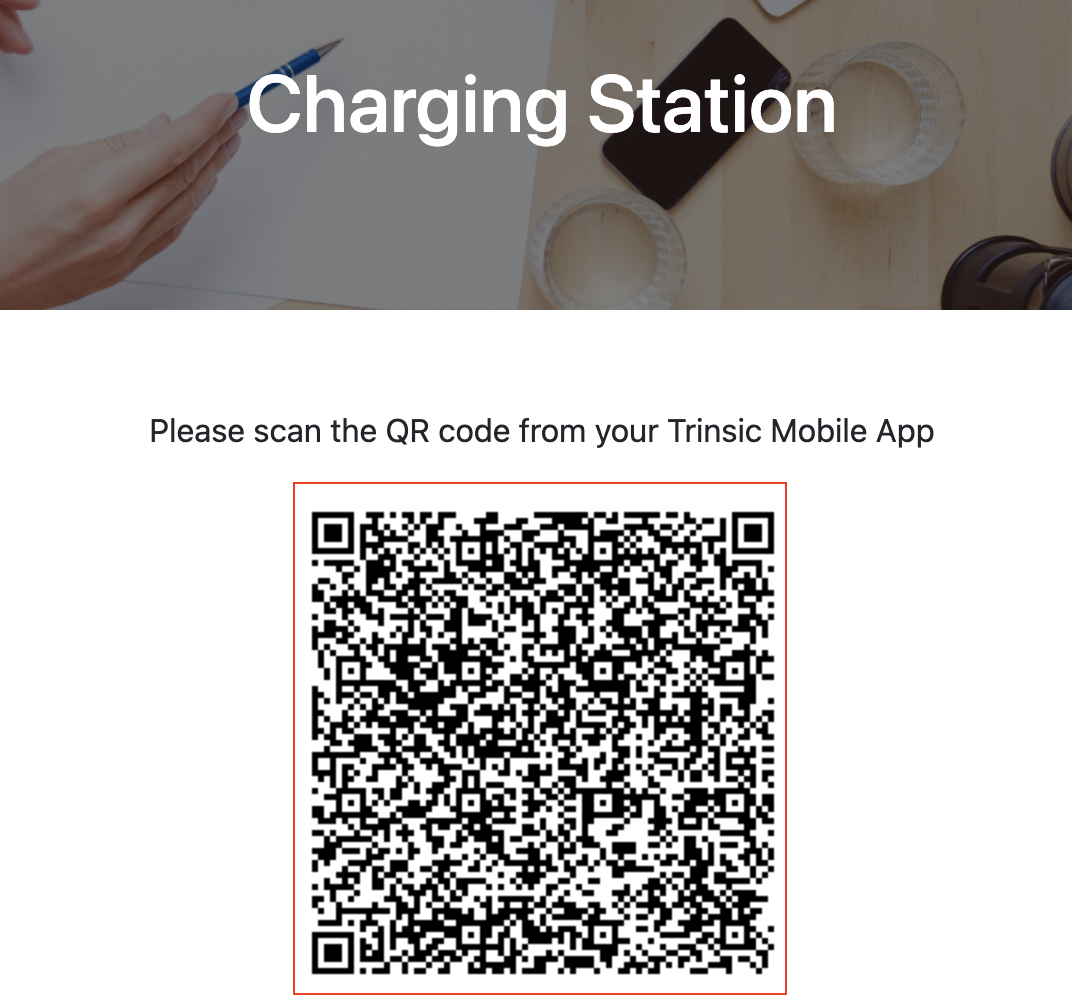
\includegraphics[width=.9\linewidth]{images/Frontend/Charging/1.1.png}
  \caption[]{Connect  to Charging Station Agent  using  QRCode}
  \label{fig:charging_screenshot_1.1}
\end{minipage}%
\begin{minipage}{.5\textwidth}
  \centering
  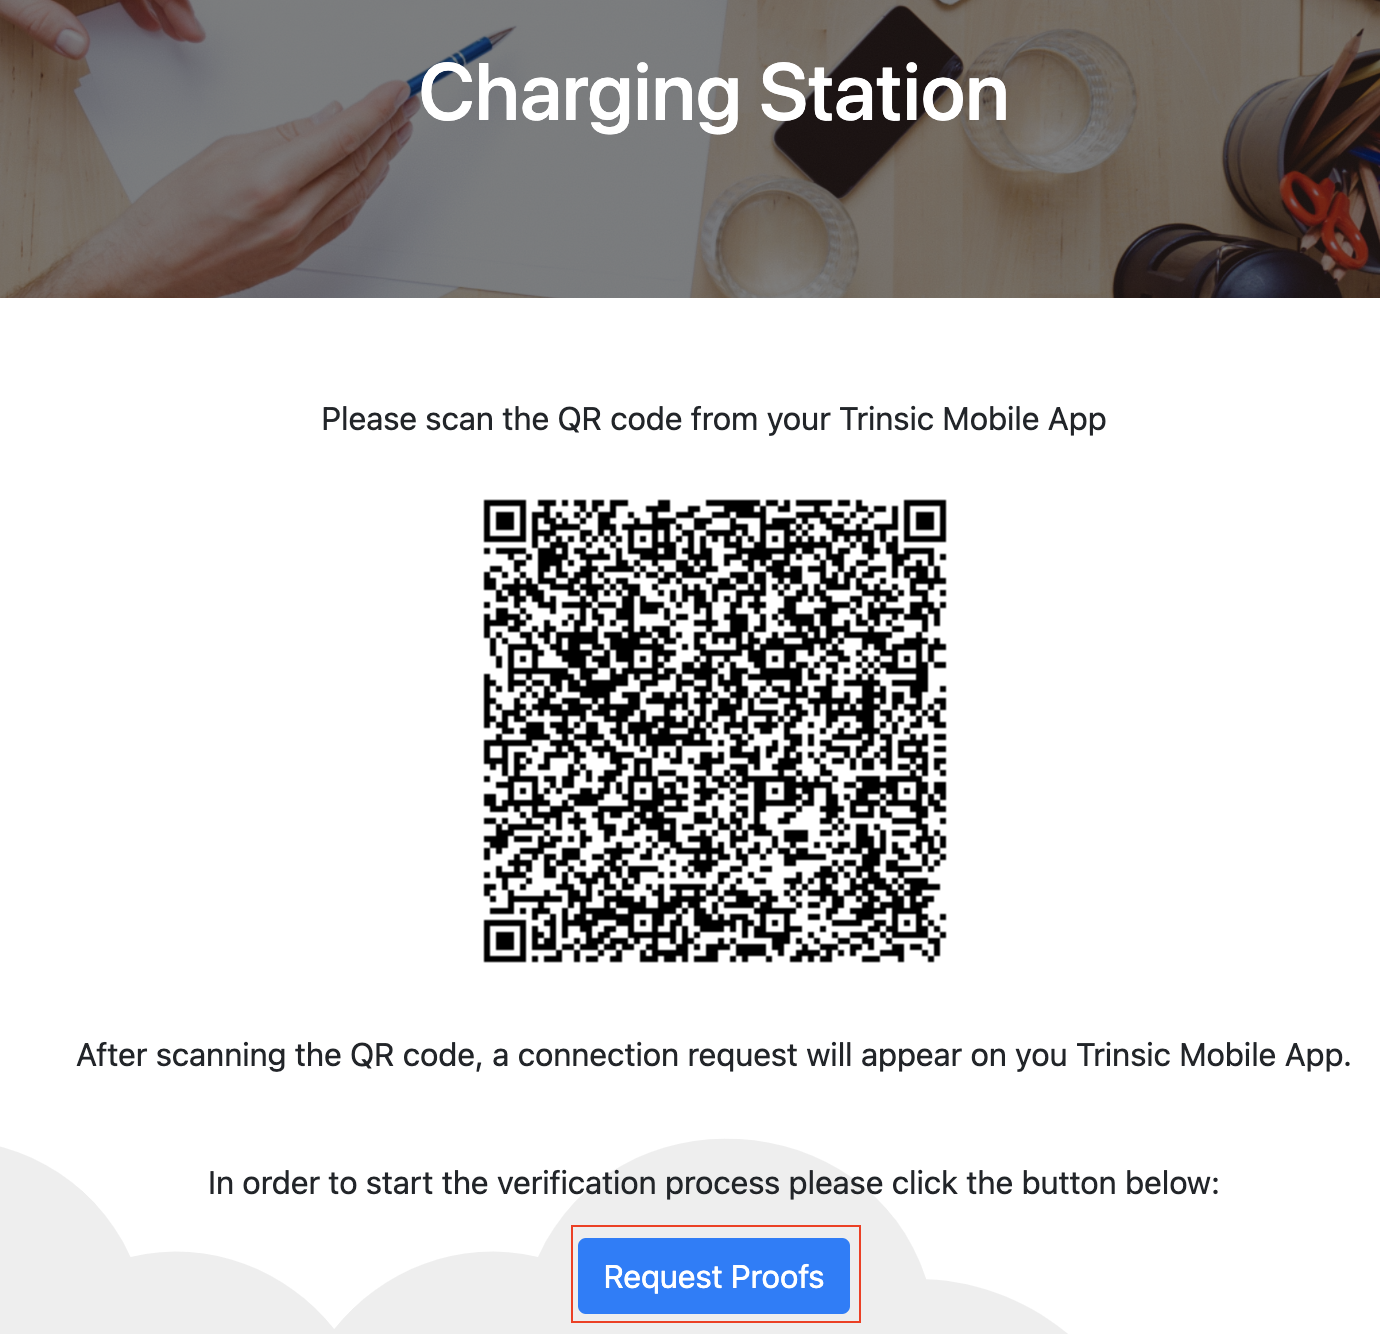
\includegraphics[width=.9\linewidth]{images/Frontend/Charging/2.png}
  \caption[]{Press the "Request Proofs" button}
  \label{fig:charging_screenshot_2}
\end{minipage}
\end{figure}

\begin{figure}[H]
\centering
\begin{minipage}{.33\textwidth}
  \centering
  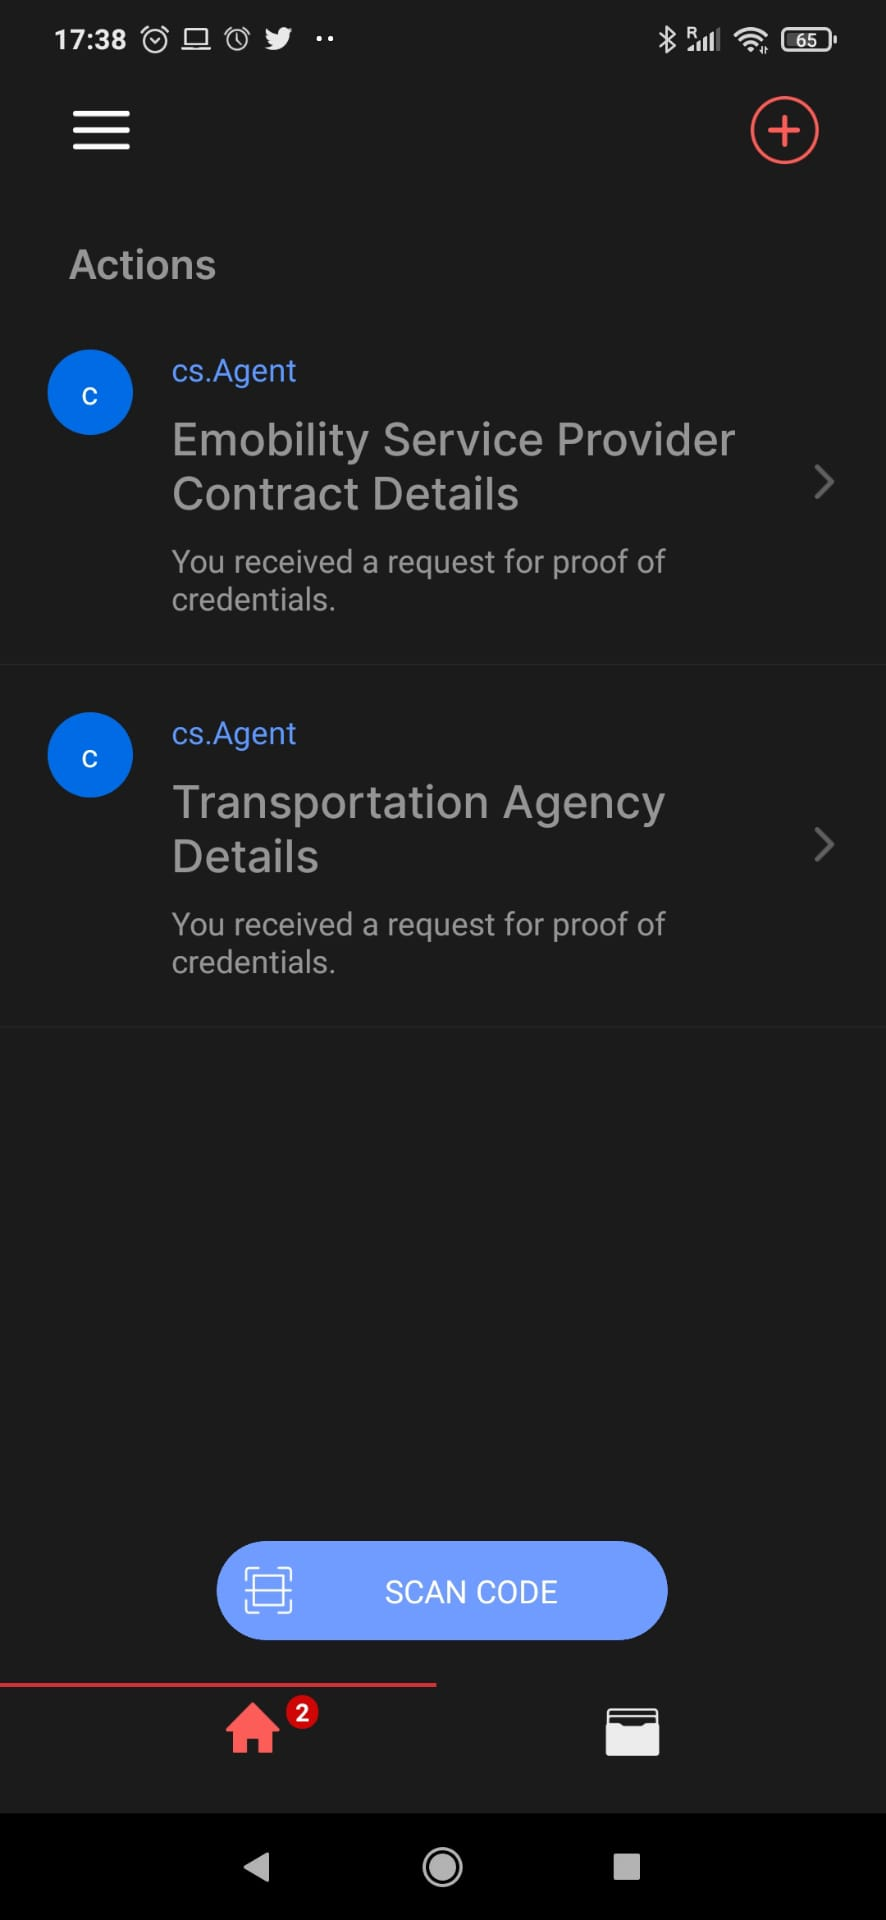
\includegraphics[width=.8\linewidth]{images/Frontend/Charging/3.0.jpeg}
  \caption[]{Receive Presentation Proof Requests on Trinsic Wallet App}
  \label{fig:charging_screenshot_3}
\end{minipage}%
\begin{minipage}{.33\textwidth}
  \centering
  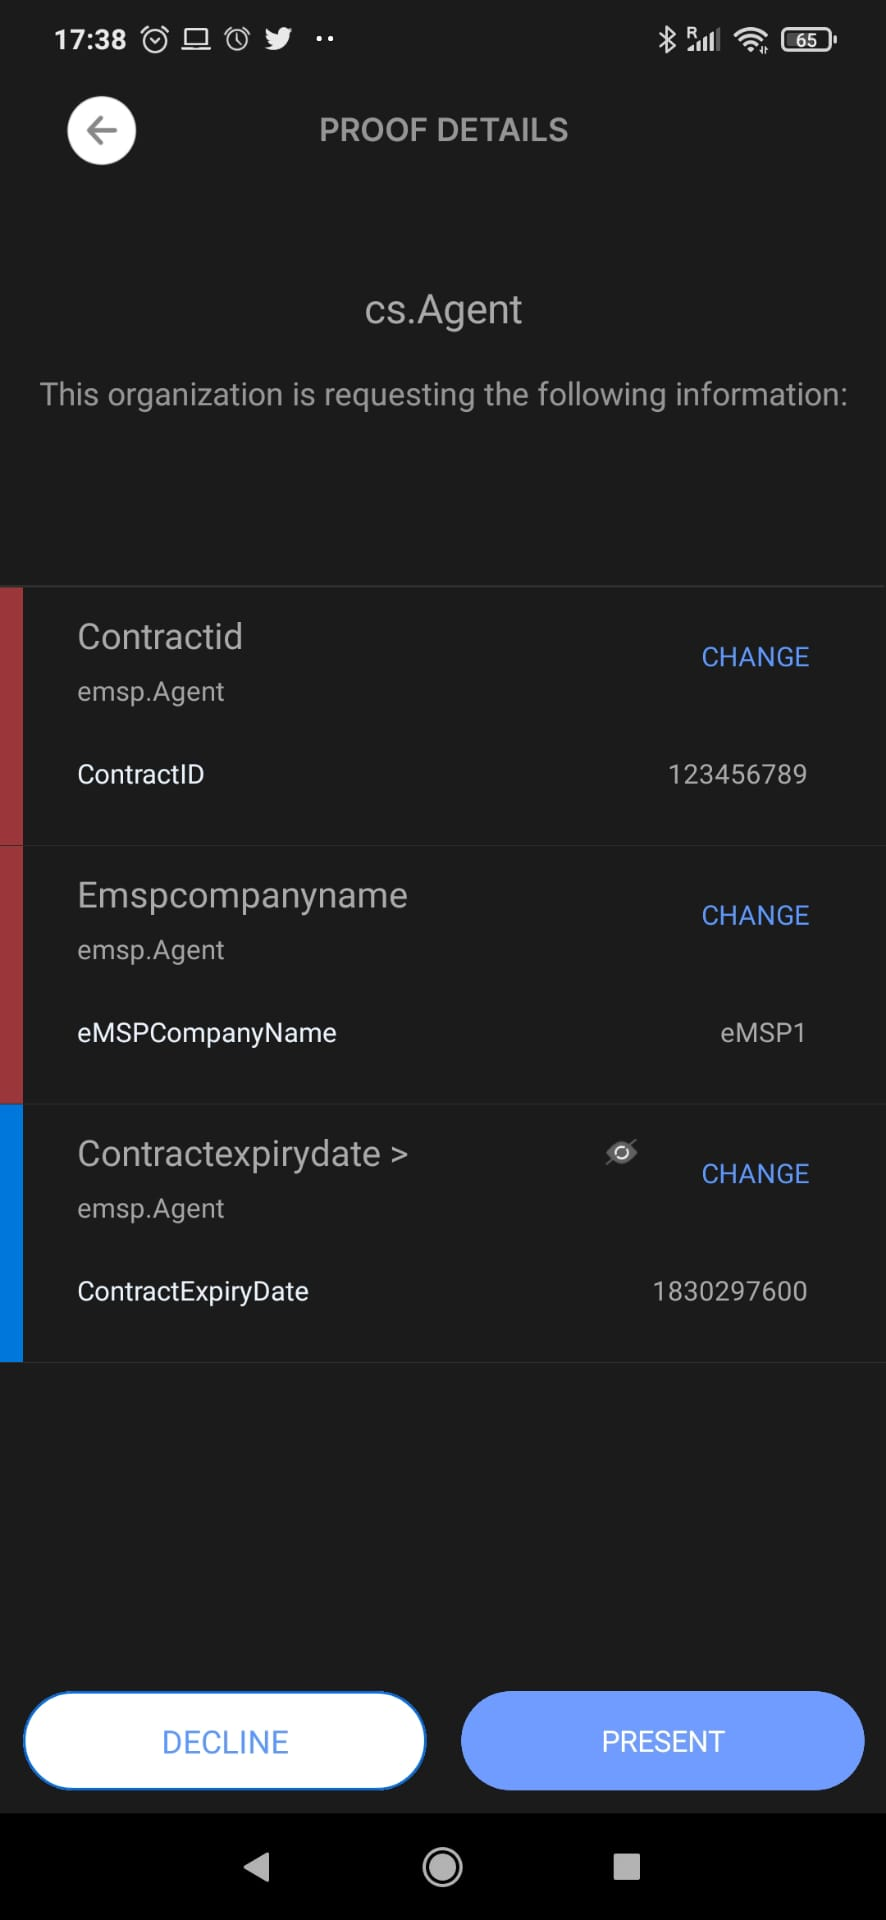
\includegraphics[width=.8\linewidth]{images/Frontend/Charging/3.1.jpeg}
  \caption[]{Present the proof for the TA-issued credential}
  \label{fig:charging_screenshot_3.1}
\end{minipage}
\begin{minipage}{.33\textwidth}
  \centering
  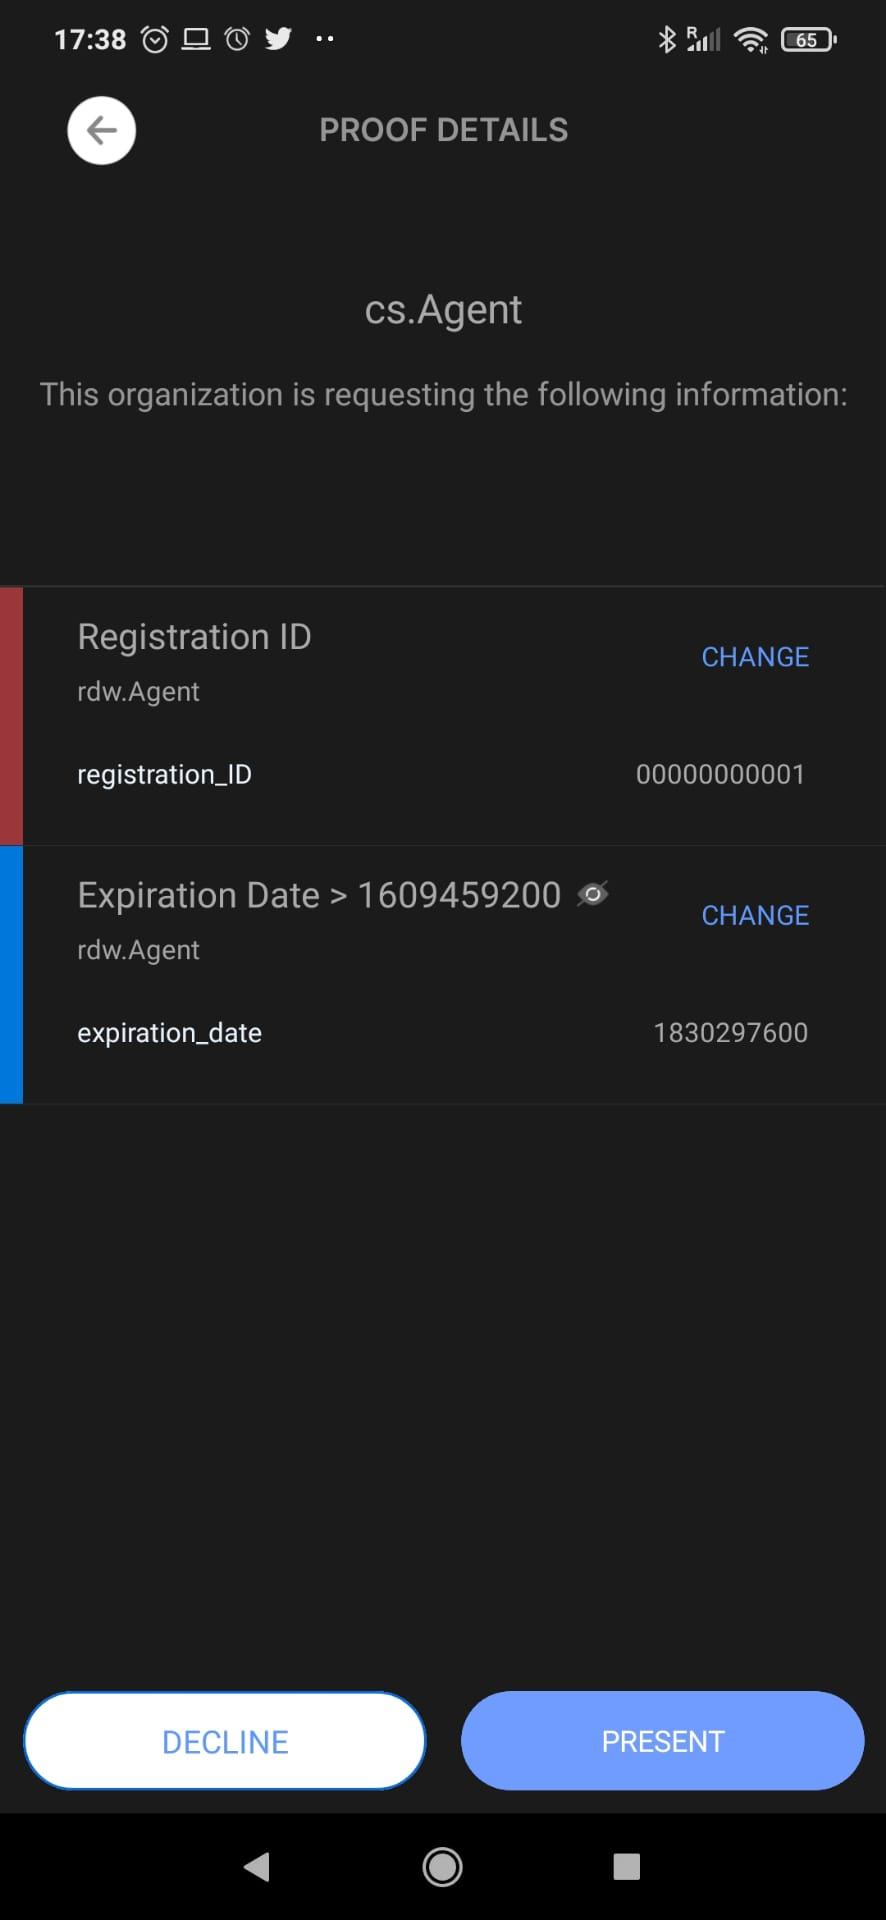
\includegraphics[width=.8\linewidth]{images/Frontend/Charging/3.2.jpeg}
  \caption[]{Present the proof for the eMSP-issued credential}
  \label{fig:charging_screenshot_3.2}
\end{minipage}
\end{figure}

\begin{figure}[H]
\centering
\begin{minipage}{.5\textwidth}
  \centering
  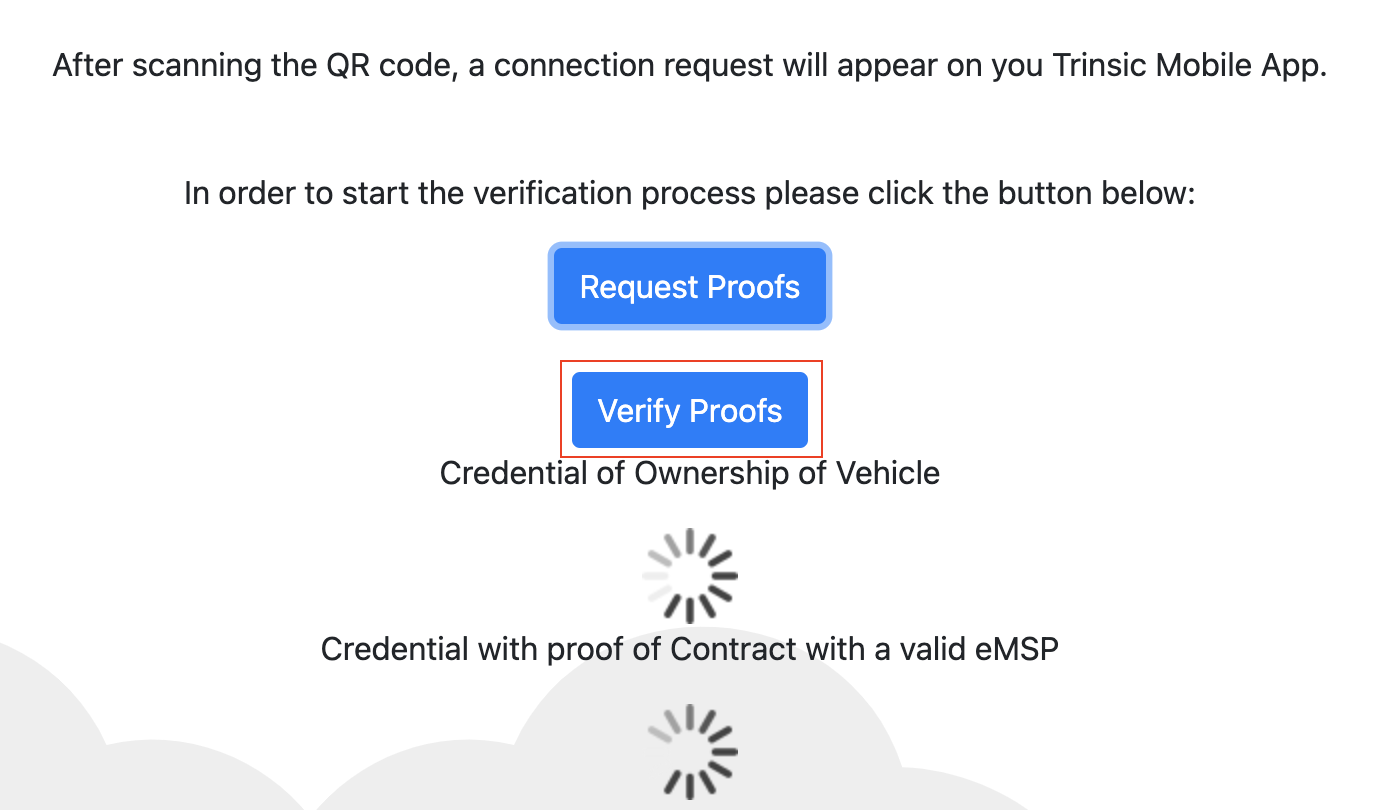
\includegraphics[width=.9\linewidth]{images/Frontend/Charging/4.png}
  \caption[]{Press the "Verify Proofs" button}
  \label{fig:charging_screenshot_4}
\end{minipage}%
\begin{minipage}{.5\textwidth}
  \centering
  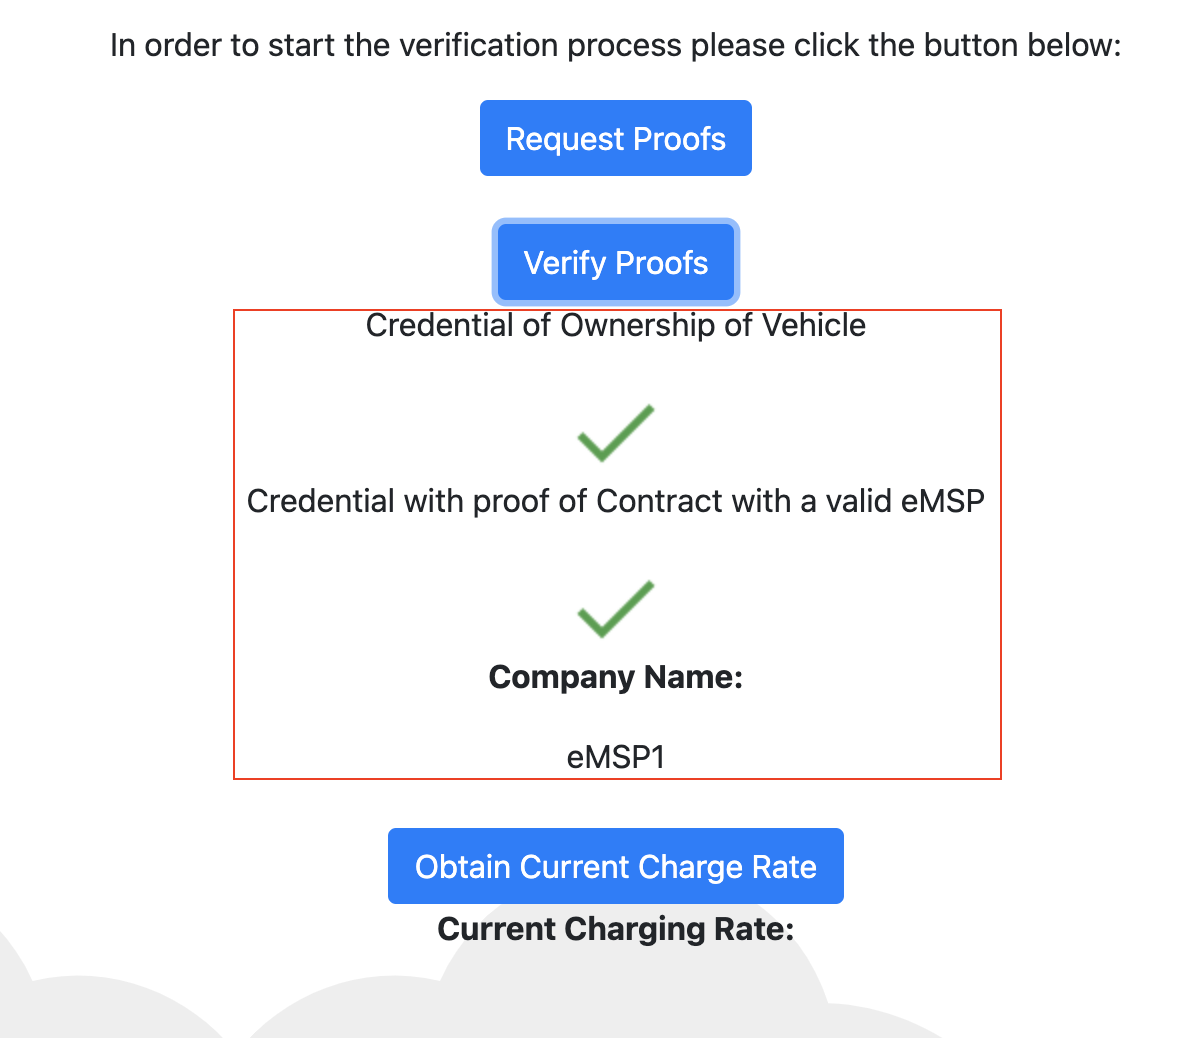
\includegraphics[width=.9\linewidth]{images/Frontend/Charging/5.png}
  \caption[]{Verify that both credentials are valid on the dashboard}
  \label{fig:charging_screenshot_5}
\end{minipage}
\end{figure}

\begin{figure}[H]
\centering
\begin{minipage}{.5\textwidth}
  \centering
  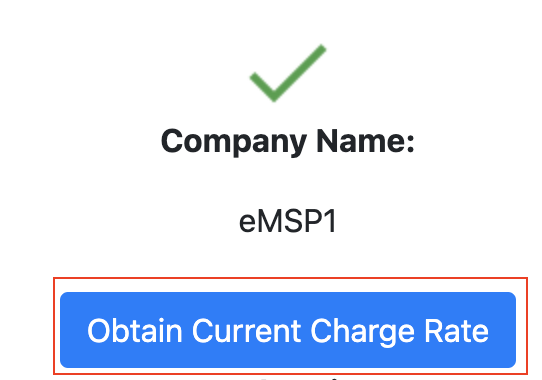
\includegraphics[width=.9\linewidth]{images/Frontend/Charging/6.png}
  \caption[]{Press the "Obtain Current Charge Rate" button}
  \label{fig:charging_screenshot_6}
\end{minipage}%
\begin{minipage}{.5\textwidth}
  \centering
  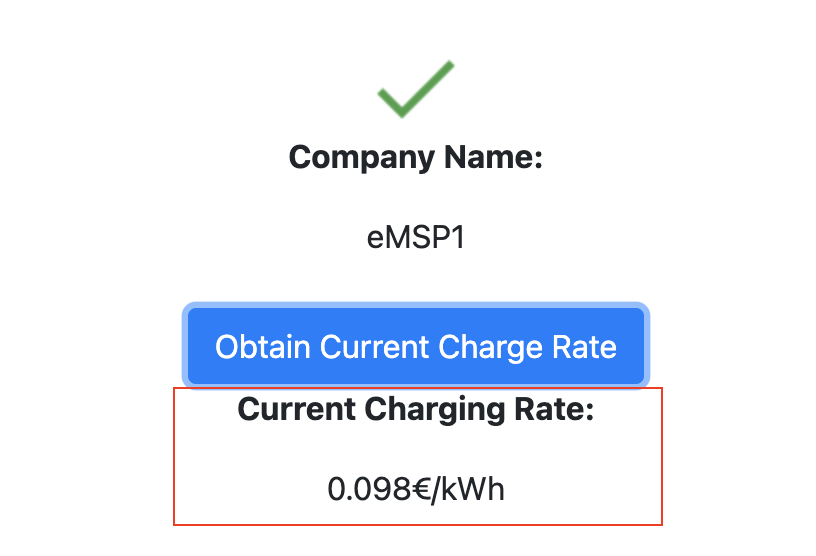
\includegraphics[width=.9\linewidth]{images/Frontend/Charging/7.png}
  \caption[]{Verify the kWh price on the dashboard}
  \label{fig:charging_screenshot_7}
\end{minipage}
\end{figure}

\begin{figure}[H]
\centering
\begin{minipage}{.5\textwidth}
  \centering
  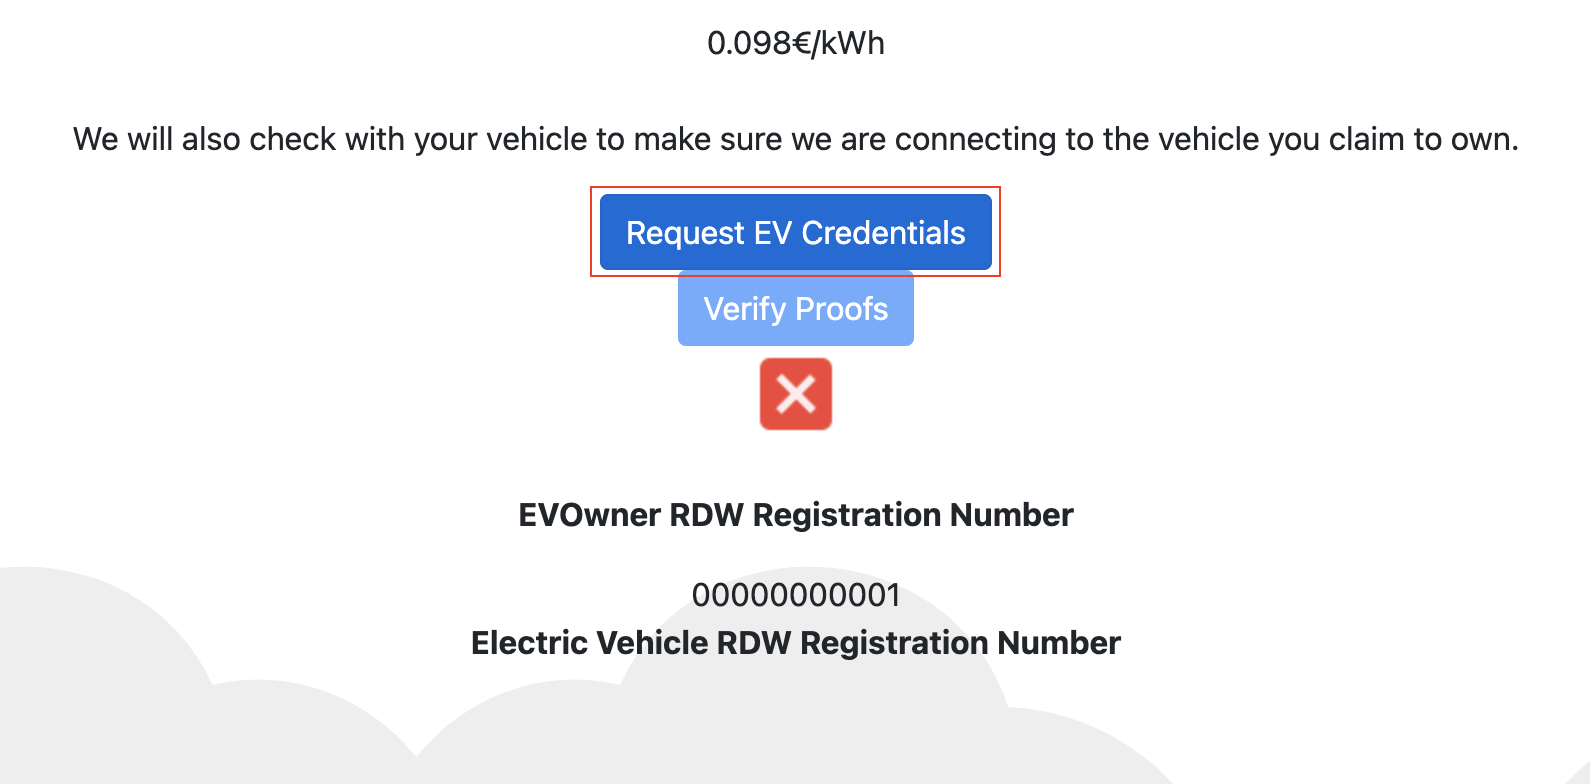
\includegraphics[width=.9\linewidth]{images/Frontend/Charging/8.png}
  \caption[]{Press the "Request EV Credentials" button}
  \label{fig:charging_screenshot_8}
\end{minipage}%
\begin{minipage}{.5\textwidth}
  \centering
  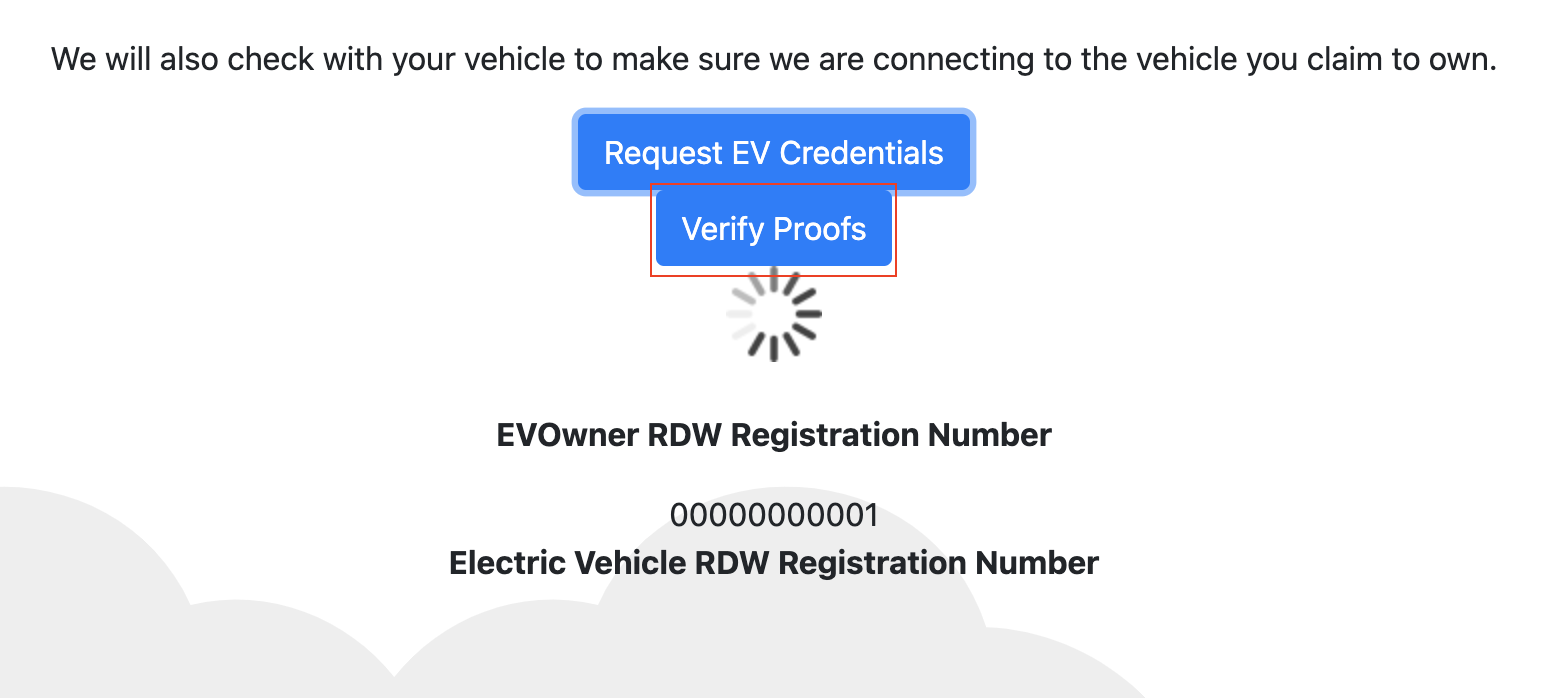
\includegraphics[width=.9\linewidth]{images/Frontend/Charging/9.png}
  \caption[]{Press the "Verify Proofs" button}
  \label{fig:charging_screenshot_9}
\end{minipage}
\end{figure}

\begin{figure}[H]
\centering
\begin{minipage}{.5\textwidth}
  \centering
  \includegraphics[width=.9\linewidth]{images/Frontend/Charging/10.png}
  \caption[]{Verify that the credential is valid on the dashboard and that the Registration Numbers match}
  \label{fig:charging_screenshot_10}
\end{minipage}%
\begin{minipage}{.5\textwidth}
  \centering
  \includegraphics[width=.9\linewidth]{images/Frontend/Charging/11.png}
  \caption[]{Press the "Start Charging" button}
  \label{fig:charging_screenshot_11}
\end{minipage}
\end{figure}

\begin{figure}[H]
\centering
\begin{minipage}{.5\textwidth}
  \centering
  \includegraphics[width=.9\linewidth]{images/Frontend/Charging/12.png}
  \caption[]{Verify that charging has occurred on the dashboard}
  \label{fig:charging_screenshot_12}
\end{minipage}%
\begin{minipage}{.5\textwidth}
  \centering
  \includegraphics[width=.9\linewidth]{images/Frontend/Charging/13.png}
  \caption[]{Press the "Issue Receipt Credential" button}
  \label{fig:charging_screenshot_13}
\end{minipage}
\end{figure}

\begin{figure}[H]
\centering
\begin{minipage}{.33\textwidth}
  \centering
  \includegraphics[width=.9\linewidth]{images/Frontend/Charging/14.0.jpeg}
  \caption[]{Receive the credential proposal on the Trinsic Wallet App}
  \label{fig:charging_screenshot_14.0}
\end{minipage}%
\begin{minipage}{.33\textwidth}
  \centering
  \includegraphics[width=.9\linewidth]{images/Frontend/Charging/14.1.jpeg}
  \caption[]{Accept the credential on the Trinsic Wallet App}
  \label{fig:charging_screenshot_14.1}
\end{minipage}
\end{figure}

\begin{figure}[H]
    \centering
    \includegraphics[width=0.6\linewidth]{images/Frontend/Charging/15.png}
    \caption[]{State of the dashboard at the end of a charging session}
    \label{fig:charging_screenshot_15}
\end{figure}

\newpage

\subsection{Aries Cloud Agent - Python Benchmark Runs}
\label{app:benchmark_runs}

In this appendix the commands used to obtain the average time of credentials are listed, followed by a small paragraph with additional information on connection times, revocation times, time to publish a schema and a credential definition.

\begin{itemize}
    \item \textit{./demo/run\_demo performance --count 1000 --mediation 2>\&1 | tee no\_revocation\_mediation\_1000.txt}
    \item \textit{./demo/run\_demo performance --count 1000 --revocation --tails-server-base-url http://host.docker.internal:6543 2>\&1 | tee revocation\_no\_mediation\_1000.txt }
    \item \textit{./demo/run\_demo performance --count 1000 2>\&1 | tee no\_revocation\_no\_mediation\_1000.txt}
    \item \textit{./demo/run\_demo performance --count 1000 --revocation --tails-server-base-url http://host.docker.internal:6543 --mediation 2>\&1 | tee revocation\_mediation\_1000.txt}
\end{itemize}

All the tests were made using the following laptop specifications:

\begin{itemize}
    \item Model Name:	MacBook Pro
    \item Model Identifier:	MacBookPro15,1
    \item Processor Name:	8-Core Intel Core i9
    \item Processor Speed:	2,3 GHz
    \item Number of Processors:	1
    \item Total Number of Cores:	8
    \item L2 Cache (per Core):	256 KB
    \item L3 Cache:	16 MB
    \item Hyper-Threading Technology:	Enabled
    \item Memory:	16 GB
    \item System Firmware Version:	1554.100.64.0.0 (iBridge: 18.16.14556.0.0,0)
    \item Docker Version: 20.10.5
\end{itemize}


\subsubsection{No Revocation + Mediation}

\begin{itemize}
    \item Startup duration: 15.14s
    \item Connect duration: 2.73s
    \item Publish duration: 14.46s
    \item Completed 1000 credential exchanges in 229.15s
    \item Average time per credential: 0.23s (4.36/s)
\end{itemize}

\subsubsection{Revocation + No Mediation}

\begin{itemize}
    \item Startup duration: 8.06s
    \item Connect duration: 0.21s
    \item Publish duration: 21.83s
    \item Completed 1000 credential exchanges in 232.92s
    \item Average time per credential: 0.23s (4.29/s)
\end{itemize}

\subsubsection{No Revocation + No Mediation}

\begin{itemize}
    \item Startup duration: 8.06s
    \item Connect duration: 0.19s
    \item Publish duration: 11.66s
    \item Completed 1000 credential exchanges in 229.45s
    \item Average time per credential: 0.23s (4.36/s)
\end{itemize}

\subsubsection{Revocation + Mediation}

\begin{itemize}
    \item Startup duration: 15.68s
    \item Connect duration: 2.72s
    \item Publish duration: 10.01s
    \item Completed 1000 credential exchanges in 263.33s
    \item Average time per credential: 0.26s (3.80/s)
\end{itemize}

\subsection{Requirement Evaluation}
\label{app:requirement_evaluation}

In this appendix, all of the requirements are discussed, presenting a table containing the requirements description, priority, status, arguments to support or contest the requirement and, when applicable, an alternative is briefly introduced to the presented arguments.

\begin{table}[H]
    \centering
    \begin{tabular}{lp{0.6\textwidth}}
         \textbf{\customlabel{evaluation:FR-1.1}{FR-1.1}} & Priority\\
         \hline\hline
         \textbf{Priority} & \textit{Must}\\
         \hline\hline
         \textbf{Status} & \greencheck\\
         \hline
         \textbf{Problem/issue} & The system must allow for an EV Owner to charge its EV at a CS\\
         \hline
         \textbf{Arguments} & The system still carries the capabilities for a client to charge its Electric Vehicle. \\
         \hline
         \textbf{Alternative(s)} & -\\
         \end{tabular}
         \caption{Evaluation of FR-1.1}
\end{table}

\begin{table}[H]
    \centering
    \begin{tabular}{lp{0.6\textwidth}}
         \textbf{\customlabel{evaluation:FR-1.2}{FR-1.2}} & Priority\\
         \hline\hline
         \textbf{Priority} & \textit{Should}\\
         \hline\hline
         \textbf{Status} &  \greencheck \\
         \hline
         \textbf{Problem/issue} & The rate at which the kWh is being sold to the EV Owner should be presented before the charging starts\\
         \hline
         \textbf{Arguments} & The current implementation of the system has the CS agent communicate to the CPO agent the company under which the client has a contract with, and receives a price rate back, displaying it to the user on the dashboard. \\
         \hline
         \textbf{Alternative(s)} & The price per kWh could be sent as a message to the user via the Trinsic Wallet App, instead of being presented on the screen.\\
         \end{tabular}
         \caption{Evaluation of FR-1.2}
\end{table}

\begin{table}[H]
    \centering
    \begin{tabular}{lp{0.6\textwidth}}
         \textbf{\customlabel{evaluation:FR-1.3}{FR-1.3}} & Priority\\
         \hline\hline
         \textbf{Priority} & \textit{Must}\\
         \hline\hline
         \textbf{Status} & \greencheck \\
         \hline
         \textbf{Problem/issue} & The EV Owner must be prompted to accept/reject the price of the kWh \\
         \hline
         \textbf{Arguments} & Although this is not actively implemented in the solution, given that the kWh price is presented to the user, it can refuse to charge the vehicle by walking out of the latter \\
         \hline
         \textbf{Alternative(s)} & In the future it would be interesting to have the user have an "accept" or "refuse" button, but that would not change the flow of the system\\
         \end{tabular}
         \caption{Evaluation of FR-1.3}
\end{table}

\begin{table}[H]
    \centering
    \begin{tabular}{lp{0.6\textwidth}}
         \textbf{\customlabel{evaluation:FR-1.4}{FR-1.4}} & Priority\\
         \hline\hline
         \textbf{Priority} & \textit{Could}\\
         \hline\hline
         \textbf{Status} & \greencheck \\
         \hline
         \textbf{Problem/issue} & At the end of a transaction, the EV Owner could receive proof of the transaction with the amount due\\
         \hline
         \textbf{Arguments} & In the new implementation of the system, the EV Owner receives a credential on his Trinsic Wallet App agent that contains information regarding the charging session.\\
         \hline
         \textbf{Alternative(s)} & -\\
         \end{tabular}
         \caption{Evaluation of FR-1.4}
\end{table}

\begin{table}[H]
    \centering
    \begin{tabular}{lp{0.6\textwidth}}
         \textbf{\customlabel{evaluation:FR-2.1}{FR-2.1}} & Priority\\
         \hline\hline
         \textbf{Priority} & \textit{Must}\\
         \hline\hline
         \textbf{Status} &  \greencheck \\
         \hline
         \textbf{Problem/issue} & A CS must belong to a CPO\\
         \hline
         \textbf{Arguments} & The Charging Station holds a credential that attests it is owned by the Charging Point Operator. \\
         \hline
         \textbf{Alternative(s)} & -\\
         \end{tabular}
         \caption{Evaluation of FR-2.1}
\end{table}

\begin{table}[H]
    \centering
    \begin{tabular}{lp{0.6\textwidth}}
         \textbf{\customlabel{evaluation:FR-2.2}{FR-2.2}} & Priority\\
         \hline\hline
         \textbf{Priority} & \textit{Must}\\
         \hline\hline
         \textbf{Status} &  \greencheck \\
         \hline
         \textbf{Problem/issue} & A CPO must have a contract with an eMSP\\
         \hline
         \textbf{Arguments} & The CPO agent holds a credential that attests a contract with an eMSP.\\
         \hline
         \textbf{Alternative(s)} & -\\
         \end{tabular}
         \caption{Evaluation of FR-2.2}
\end{table}

\begin{table}[H]
    \centering
    \begin{tabular}{lp{0.6\textwidth}}
         \textbf{\customlabel{evaluation:FR-2.3}{FR-2.3}} & Priority\\
         \hline\hline
         \textbf{Priority} & \textit{Must}\\
         \hline\hline
         \textbf{Status} &  \greencheck \\
         \hline
         \textbf{Problem/issue} & A CPO must have a contract with an EP to provide power to its Charging Stations\\
         \hline
         \textbf{Arguments} & The CPO agent holds a credential that attests a contract with an EP. \\
         \hline
         \textbf{Alternative(s)} & -\\
         \end{tabular}
         \caption{Evaluation of FR-2.3}
\end{table}

\begin{table}[H]
    \centering
    \begin{tabular}{lp{0.6\textwidth}}
         \textbf{\customlabel{evaluation:FR-3.1}{FR-3.1}} & Priority\\
         \hline\hline
         \textbf{Priority} & \textit{Should}\\
         \hline\hline
         \textbf{Status} &  \greencheck \\
         \hline
         \textbf{Problem/issue} & EV Owners should prove they are the owners of their EV to a CS\\
         \hline
         \textbf{Arguments} & In the current implementation of the system, the EV Owner and the EV both have a credential provided by the Transportation Agency that links both by a registrationID, as seen in Section~\ref{paragraph:ev_owner_and_ev_interactions_with_ssi}. \\
         \hline
         \textbf{Alternative(s)} & The fact that the link between the EV and the EV Owner is made with the use of a unique identifier might impose privacy-damaging practices, that need to be evaluated at a later stage.\\
         \end{tabular}
         \caption{Evaluation of FR-3.1}
\end{table}
\begin{table}[H]
    \centering
    \begin{tabular}{lp{0.6\textwidth}}
         \textbf{\customlabel{evaluation:FR-3.2}{FR-3.2}} & Priority\\
         \hline\hline
         \textbf{Priority} & \textit{Must}\\
         \hline\hline
         \textbf{Status} &  \greencheck\\
         \hline
         \textbf{Problem/issue} & EV Owners must attest they have a valid contract with an eMSP that the CS's CPO has a contract with\\
         \hline
         \textbf{Arguments} & The EV Owner is given a credential from the eMSP that attests the contract between the two, and is presented at a Charging Station for verification. \\
         \hline
         \textbf{Alternative(s)} & -\\
         \end{tabular}
         \caption{Evaluation of FR-3.2}
\end{table}

\begin{table}[H]
    \centering
    \begin{tabular}{lp{0.6\textwidth}}
         \textbf{\customlabel{evaluation:FR-3.3}{FR-3.3}} & Priority\\
         \hline\hline
         \textbf{Priority} & \textit{Could}\\
         \hline\hline
         \textbf{Status} &  \redcheckk\\
         \hline
         \textbf{Problem/issue} & An EV Owner could be made aware that the CS belongs to the CPO it claims\\
         \hline
         \textbf{Arguments} & Although the Charging Station holds a credential that attests it is owned by a specific CPO, that credential has not been included in the proof-of-concept, but could be added easily later on, with the support of a better mobile agent. \\
         \hline
         \textbf{Alternative(s)} & -\\
         \end{tabular}
         \caption{Evaluation of FR-3.3}
\end{table}
\begin{table}[H]
    \centering
    \begin{tabular}{lp{0.6\textwidth}}
         \textbf{\customlabel{evaluation:FR-3.4}{FR-3.4}} & Priority\\
         \hline\hline
         \textbf{Priority} & \textit{Should}\\
         \hline\hline
         \textbf{Status} &  \greencheck \\
         \hline
         \textbf{Problem/issue} & The process of setting up the connection and verifying credentials should be executed with the least EV Owner intervention as possible.\\
         \hline
         \textbf{Arguments} & The process of establishing a connection and verifying credentials has been reduced to a maximum of steps that abide to all of the requirements and does not incur in problem for the users, according to the data extracted from the experts evaluation in Section~\ref{subsec:qualitative_evaluatin_from_domain_experts}. \\
         \hline
         \textbf{Alternative(s)} & -\\
         \end{tabular}
         \caption{Evaluation of FR-3.4}
\end{table}

\begin{table}[H]
    \centering
    \begin{tabular}{lp{0.6\textwidth}}
         \textbf{\customlabel{evaluation:FR-4.1}{FR-4.1}} & Priority\\
         \hline\hline
         \textbf{Priority} & \textit{Must}\\
         \hline\hline
         \textbf{Status} &  \greencheck \\
         \hline
         \textbf{Problem/issue} & An EV and the information regarding its EV Owner must be registered with the TA in order for the EV to be on the roads and to be charged at a CS\\
         \hline
         \textbf{Arguments} & The EV and its EV Owner are registered at the Transportation Agency and are provided with credentials that attest these claims. \\
         \hline
         \textbf{Alternative(s)} & -\\
         \end{tabular}
         \caption{Evaluation of FR-4.1}
\end{table}

\begin{table}[H]
    \centering
    \begin{tabular}{lp{0.6\textwidth}}
         \textbf{\customlabel{evaluation:FR-5.1}{FR-5.1}} & Priority\\
         \hline\hline
         \textbf{Priority} & \textit{Must}\\
         \hline\hline
         \textbf{Status} &  \greencheck\\
         \hline
         \textbf{Problem/issue} & The system must not write PII in a publicly accessible data repository\\
         \hline
         \textbf{Arguments} & With the usage of the Hyperledger Indy and the Hyperledger Aries ecosystems, it is guaranteed that no Personally Identifiable Information is written on the blockchain, and that the data is only stored in wallets held by each entity as seen in Section~\ref{subsec:what_information_goes_onto_the_DLT?}. \\
         \hline
         \textbf{Alternative(s)} & -\\
         \end{tabular}
         \caption{Evaluation of FR-5.1}
\end{table}

\begin{table}[H]
    \centering
    \begin{tabular}{lp{0.6\textwidth}}
         \textbf{\customlabel{evaluation:FR-5.2}{FR-5.2}} & Priority\\
         \hline\hline
         \textbf{Priority} & \textit{Must}\\
         \hline\hline
         \textbf{Status} &  \greencheck \\
         \hline
         \textbf{Problem/issue} & Every credential issued must be verifiable using cryptographic proof\\
         \hline
         \textbf{Arguments} & With the cryptographic capabilities provided by Hyperledger Ursa to the solution, it is guaranteed that this solution employs state of the art cryptography practices, as seen in Section~\ref{subsubsec:hyperledger_indy_sovrin}.\\
         \hline
         \textbf{Alternative(s)} & -\\
         \end{tabular}
         \caption{Evaluation of FR-5.2}
\end{table}

\begin{table}[H]
    \centering
    \begin{tabular}{lp{0.6\textwidth}}
         \textbf{\customlabel{evaluation:FR-6.1}{FR-6.1}} & Priority\\
         \hline\hline
         \textbf{Priority} & \textit{Must}\\
         \hline\hline
         \textbf{Status} &  \redcheckk\\
         \hline
         \textbf{Problem/issue} & An EV Owner must be able to delegate (temporary) possession of its EV to another driver\\
         \hline
         \textbf{Arguments} & In the current implementation of the ACA-Py agents, there is a work in progress to implement delegated credentials, which will mitigate this requirement in a near future. \\
         \hline
         \textbf{Alternative(s)} & Issue a credential to each individual that will be the driver of the vehicle, which is impractical in real-life scenarios.\\
         \end{tabular}
         \caption{Evaluation of FR-6.1}
\end{table}


\begin{table}[H]
    \centering
    \begin{tabular}{lp{0.6\textwidth}}
         \textbf{\customlabel{evaluation:NFR-1.1}{NFR-1.1}} & Priority\\
         \hline\hline
         \textbf{Priority} & \textit{Must}\\
         \hline\hline
         \textbf{Status} & \textit{\textbf{-}}\\
         \hline
         \textbf{Problem/issue} & The system must scale according to the growth of the market. Supposing an adoption in the Dutch Market (300k EVs in 2020), the system must be able to support this number of vehicles and the estimated growth (3M EVs by 2030)\\
         \hline
         \textbf{Arguments} & This requirement can be validated with the results obtained in Section~\ref{subsec:benchmark_hyperledger_indy_and_aries} since the Sovrin network is able to withstand the current load without a loss of information. But for this requirement to be validated more tests need to be performed to the network to adjust the number of nodes needed to withstand such system scale. \\
         \hline
         \textbf{Alternative(s)} & -\\
         \end{tabular}
         \caption{Evaluation of NFR-1.1}
\end{table}

\begin{table}[H]
    \centering
    \begin{tabular}{lp{0.6\textwidth}}
         \textbf{\customlabel{evaluation:NFR-2.1}{NFR-2.1}} & Priority\\
         \hline\hline
         \textbf{Priority} & \textit{Should}\\
         \hline\hline
         \textbf{Status} &  \greencheck\\
         \hline
         \textbf{Problem/issue} & The system should be able to kickstart the charging process in a reasonable amount of time (no longer than the time required without VCs, less than 1 minute)\\
         \hline
         \textbf{Arguments} & The system has been timed in the charging station dashboard, and the process of charging could be started with less than 1 minute, depending on the user expertise with the technology. From the experts evaluation, the user experience has not been affected according to the results on Section~\ref{subsec:qualitative_evaluatin_from_domain_experts} \\
         \hline
         \textbf{Alternative(s)} & -\\
         \end{tabular}
         \caption{Evaluation of NFR-2.1}
\end{table}

\begin{table}[H]
    \centering
    \begin{tabular}{lp{0.6\textwidth}}
         \textbf{\customlabel{evaluation:NFR-2.2}{NFR-2.2}} & Priority\\
         \hline\hline
         \textbf{Priority} & \textit{Must}\\
         \hline\hline
         \textbf{Status} &  \greencheck\\
         \hline
         \textbf{Problem/issue} & The system must withstand multiple users accessing the system at the same time, with no loss of information.\\
         \hline
         \textbf{Arguments} & This requirement is assessed on a theoretical level, since no tests were made with concurrent agents performing the same flow. But, the capability of the system to handle concurrent users depends on the Hyperledger Indy network and not the agents, since each charging station will have one agent each, and therefore only have one session happening at the same time, which has been tested and proven to work. The network can withstand multiple agents writing at the same time as seen by the results on Section~\ref{subsec:benchmark_hyperledger_indy_and_aries}.  \\
         \hline
         \textbf{Alternative(s)} & -\\
         \end{tabular}
         \caption{Evaluation of NFR-2.2}
\end{table}

\begin{table}[H]
    \centering
    \begin{tabular}{lp{0.6\textwidth}}
         \textbf{\customlabel{evaluation:NFR-2.3}{NFR-2.3}} & Priority\\
         \hline\hline
         \textbf{Priority} & \textit{Must}\\
         \hline\hline
         \textbf{Status} &  \greencheck \\
         \hline
         \textbf{Problem/issue} & The user must be presented with information on how to engage with the CS in less than 5 seconds.\\
         \hline
         \textbf{Arguments} & As soon as the user arrives at the Charging Station, a call is made to the Charging Station agent to generate an invitation for the EV Owner to connect. This action occurs asynchronously and takes less than 2 seconds to appear.\\
         \hline
         \textbf{Alternative(s)} & -\\
         \end{tabular}
         \caption{Evaluation of NFR-2.3}
\end{table}

\begin{table}[H]
    \centering
    \begin{tabular}{lp{0.6\textwidth}}
         \textbf{\customlabel{evaluation:NFR-2.4}{NFR-2.4}} & Priority\\
         \hline\hline
         \textbf{Priority} & \textit{Should}\\
         \hline\hline
         \textbf{Status} &  \greencheck \\
         \hline
         \textbf{Problem/issue} & The process of validation the client’s credentials should not take longer than the original method (designed for 2 seconds, with the worst case scenario being 30 seconds)\\
         \hline
         \textbf{Arguments} & Following the work made on Section~\ref{subsec:benchmark_hyperledger_indy_and_aries} regarding the benchmarks of the ACA-Py agents and the results, this requirement can be marked as fulfilled. \\
         \hline
         \textbf{Alternative(s)} & -\\
         \end{tabular}
         \caption{Evaluation of NFR-2.4}
\end{table}

\begin{table}[H]
    \centering
    \begin{tabular}{lp{0.6\textwidth}}
         \textbf{\customlabel{evaluation:NFR-3.1}{NFR-3.1}} & Priority\\
         \hline\hline
         \textbf{Priority} & \textit{Should}\\
         \hline\hline
         \textbf{Status} &  \greencheck\\
         \hline
         \textbf{Problem/issue} & The system should be constantly updated to mitigate the risk of quantum-attacks, by employing state-of-the art cryptography\\
         \hline
         \textbf{Arguments} & The current implementation of the Hyperledger Indy and Aries frameworks are based on another project from the Hyperledger ecosystem, Ursa. This project is the cryptographic core of both projects and is constantly updated to provide state-of-the-art security to both solutions.  \\
         \hline
         \textbf{Alternative(s)} & -\\
         \end{tabular}
         \caption{Evaluation of NFR-3.1}
\end{table}

\begin{table}[H]
    \centering
    \begin{tabular}{lp{0.6\textwidth}}
         \textbf{\customlabel{evaluation:NFR-3.2}{NFR-3.2}} & Priority\\
         \hline\hline
         \textbf{Priority} & \textit{Must}\\
         \hline\hline
         \textbf{Status} & \textbf{-}\\
         \hline
         \textbf{Problem/issue} & The system must comply with Dutch regulations, including GDPR\\
         \hline
         \textbf{Arguments} & Although blockchain and the information that gets written to the DLT, as discussed in Section~\ref{subsec:what_information_goes_onto_the_DLT?}, do provide GDPR compliance, two matters on the solution do not. The two latter have been assessed in the Limitations chapter (Section~\ref{subsubsec:limitations}) and hence the requirement has been marked with \textbf{"-"}. \\
         \hline
         \textbf{Alternative(s)} & Discussed in the Limitations chapter.\\
         \end{tabular}
         \caption{Evaluation of NFR-3.2}
\end{table}

\begin{table}[H]
    \centering
    \begin{tabular}{lp{0.6\textwidth}}
         \textbf{\customlabel{evaluation:NFR-3.3}{NFR-3.3}} & Priority\\
         \hline\hline
         \textbf{Priority} & \textit{Must}\\
         \hline\hline
         \textbf{Status} &  \greencheck\\
         \hline
         \textbf{Problem/issue} & The system must be protected against forgery of identity, so that in the case of theft of identity the malicious party cannot use the system\\
         \hline
         \textbf{Arguments} & The core principals of SSI and the Verifiable Credentials allow to comply with this requirement, since each credential is cryptographically signed and there is no way to tamper this information or forge it, unless a wallet is taken hostage by a malicious party. But even in these circumstances, biometrics could be used as a Two-Factor Authentication method. \\
         \hline
         \textbf{Alternative(s)} & -\\
         \end{tabular}
         \caption{Evaluation of NFR-3.3}
\end{table}

\begin{table}[H]
    \centering
    \begin{tabular}{lp{0.6\textwidth}}
         \textbf{\customlabel{evaluation:NFR-4.1}{NFR-4.1}} & Priority\\
         \hline\hline
         \textbf{Priority} & \textit{Must}\\
         \hline\hline
         \textbf{Status} &  \greencheck\\
         \hline
         \textbf{Problem/issue} & A CS must have an active internet connection to authenticate the EV Owner\\
         \hline
         \textbf{Arguments} & Although not actively evaluated, in Section~\ref{subsubsec:evaluation_non_functional_requirements} a discussion is conducted to why this requirement can be fulfilled if applied in the Netherlands.\\
         \hline
         \textbf{Alternative(s)} & Perform more research to assess the current state of charging station connectivity in more regions where this solution might be applied. \\
         \end{tabular}
         \caption{Evaluation of NFR-4.1}
\end{table}

\begin{table}[H]
    \centering
    \begin{tabular}{lp{0.6\textwidth}}
         \textbf{\customlabel{evaluation:NFR-4.2}{NFR-4.2}} & Priority\\
         \hline\hline
         \textbf{Priority} & \textit{Must}\\
         \hline\hline
         \textbf{Status} &  \greencheck\\
         \hline
         \textbf{Problem/issue} & The systems implementation must allow for as many agent implementations as possible, opting for solutions that favor interoperability\\
         \hline
         \textbf{Arguments} & This requirement is fulfilled since the goal of Hyperledger Indy and Aries is to provide an interoperable ecosystem that is not vendor-locked. Any agent that complies with the current Verifiable Credentials standards is capable of interacting with the Hyperledger Indy network, and that is why this requirement is fulfilled. \\
         \hline
         \textbf{Alternative(s)} & -\\
         \end{tabular}
         \caption{Evaluation of NFR-4.2}
\end{table}

\begin{table}[H]
    \centering
    \begin{tabular}{lp{0.6\textwidth}}
         \textbf{\customlabel{evaluation:NFR-4.3}{NFR-4.3}} & Priority\\
         \hline\hline
         \textbf{Priority} & \textit{Must}\\
         \hline\hline
         \textbf{Status} &  \greencheck\\
         \hline
         \textbf{Problem/issue} & The system must offer a 97\% uptime guarantee\\
         \hline
         \textbf{Arguments} & Following the evaluation performed on the Hyperledger Indy network in Section~\ref{subsec:benchmark_hyperledger_indy_and_aries}, the current best example of an Indy network has more than 97\% uptime, which leads to believe that it is capable of handling this availability requirements.\\
         \hline
         \textbf{Alternative(s)} & -\\
         \end{tabular}
         \caption{Evaluation of NFR-4.3}
\end{table}


\newpage



\end{document}